2003/WITH PROOF

\documentclass{article}
\title{Analysis I}
\author{Prof. T.~W.~K\"orner}
\date{Lent 2003}
\usepackage{amssymb}
\usepackage{amsmath}
\usepackage{amsthm}
\usepackage{pifont}
\usepackage{cancel}
\usepackage{hyperref}
\usepackage{graphicx}
\hypersetup{colorlinks=true, linkcolor=red}

\theoremstyle{definition} 
\newtheorem{AYTheorem}{Theorem}[section]
\newtheorem{AYLemma}[AYTheorem]{Lemma}
\newtheorem{AYCorollary}[AYTheorem]{Corollary}
\newtheorem{AYDefinition}[AYTheorem]{Definition}
\newtheorem{AYExample}[AYTheorem]{Example}
\newtheorem{AYExercise}[AYTheorem]{Exercise}
\newtheorem{AYConvention}[AYTheorem]{Convention}
\newtheorem{AYStatement}[AYTheorem]{Statement}
\newtheorem{AYFact}[AYTheorem]{Fact}
\newtheorem{AYAxiom}[AYTheorem]{Axiom}
\setlength{\parindent}{0pt}




%Theorem~\ref{ArchimedesAxiom} shows that there is no `exotic' real number $\gimel$ say (to choose an exotic symbol) with the property that $1/n > \gimel$ for all integers $n \geq 1$ yet $\gimel >0$ (that is, $\gimel$ is strictly positive and yet smaller than all strictly positive rationals). There exist number systems with such exotic numbers (the famous `non-standard analysis' of Abraham Robinson and the `surreal numbers' of Conway constitute two such systems) but, just as the rationals are, in some sense, too small a system for the standard theorems of analysis to hold so these non-Archimedean systems are, in some sense, too big. Archimedes and  Eudoxus realised the need for an axiom to show that there is no exotic number $\daleth$ bigger than any integer\footnote{Footnote for passing historians, this is a course in mathematics.} (i.e. $\daleth > n$ for all integers $n\geq 1$; to see the connection with our form of the axiom consider $\gimel = 1/ \daleth$). However, in spite of its name, what was an axiom for Archimedes is a theorem for us.

%Note: Work as much as possible with $\sum_1^N a_n$ and as little as possible with $\sum_1^\infty a_n$ until you know that $\sum_1^\infty a_n$ exists\\















We proved the intermediate value theorem (Theorem~\ref{IntermediateValueTheorem}) by lion hunting. We prove the next two theorems by using the Bolzano-Weierstrass Theorem (Theorem~\ref{BolzanoWeierstrassTheorem}). Again the results are very important and I can see no objection to learning the proofs as a model. 

\begin{AYTheorem}
If $f : [a,b] \rightarrow \mathbb{R}$ is continuous then we can find an $M$ such that $|f(x)| \leq M$ for all $x \in [a,b]$.
\end{AYTheorem}

\begin{proof}
Note that this needs to be on a closed interval, on $(0, 1) \ f: x \mapsto \frac{1}{x}$ is unbounded

Suppose $f$ is unbounded

Then we can find $x_n \in [a, b]$ such that $|f(x_n)| \geq n$

The $x_n$ lie in a bounded interval so they have a convergent subsequence $x_{n(j)} \rightarrow \alpha$ say. Since $x_{n(j)} \leq b, \alpha \leq b$ and since $x_{n(j)} \geq a, \alpha \geq a$ so $\alpha \in [a, b]$

Now $f$ is continuous at $\alpha$ so $\exists \ \delta > 0$ such that $|f(\alpha) - f(x)| < 1 \ \forall |x-\alpha| < \delta$

$x \in [a, b]$ so $|f(x)| \leq |f(\alpha) + 1| \ \forall |x-\alpha| < \delta, x \in [a, b]$

But $x_{n(j)} \rightarrow \alpha$. So $\exists J$ such that if $j \geq J \ |x_{n(j)} - \alpha| < \delta$

so $n(j) \leq |f(x_{n(j)}| \leq |f(\alpha)| + 1 \ \forall j \geq J$ \#

Thus $f$ must be bounded
\end{proof}

In other words a continuous function on a closed bounded interval is bounded. We improve this result in the next theorem.

\begin{AYTheorem}
\label{BoundedContinuousAttainsBounds}
If $f : [a,b] \rightarrow \mathbb{R}$ is continuous then we can find $x_1, x_2 \in [a,b]$ such that
\begin{equation*}
f(x_1) \leq f(x) \leq f(x_2)
\end{equation*}
for all $x\in[a,b]$.
\end{AYTheorem}

\begin{proof}
Start by observing that $\{f(x) : x \in [a, b]\}$ is a non-empty bounded set, so it has a supremum $M$. What we need to show is that $\exists \alpha \in [a, b]$ such that $f(\alpha) = M$

Since $M$ is the supremum of $\{f(x) : x \in [a, b]\}$ we can certainly find $x_n \in [a, b]$ such that $f(x_n) \geq M - \frac{1}{n}$ (if not, then $(M - \frac{1}{n})$ would be an upper bound, but $M$ is the least upper bound). Automatically $M \geq f(x_n)$

By Bolzano-Weierstrass there is a convergenet subsequence $x_{n(j)} \rightarrow \alpha$. As before $\alpha \in [a, b]$ and $f(x_{n(j)}) \rightarrow f(\alpha)$. But $M \geq f(x_{n(j)}) \geq M - \frac{1}{n(j)}$, so $f(x_{n(j)}) \rightarrow M$ so $f(\alpha) = M$
\end{proof}

In other words a continuous function on a closed bounded interval is bounded and attains its bounds. 


%%%%%%%%%%%%%%%%%%%%%%%


\section{Differentiation}

In this section it will be useful to have another type of limit.

\begin{AYDefinition}
Let $E$ be a subset of $\mathbb{R}$, $f$ be some function from $E$ to $\mathbb{R}$, and $x$ some point of $E$. If $l \in \mathbb{R}$ we say that $f(y) \rightarrow l$ as $y \rightarrow x$ [or, if we wish to emphasise the restriction to $E$
that $f(y) \rightarrow l$ as $y \rightarrow x$ through values $y \in E$] if, given $\epsilon > 0$, we can find a $\delta(\epsilon)>0$ [read `a delta depending on epsilon'] such that
\begin{equation*}
|f(y)-l|<\epsilon
\end{equation*}
for all $y \in E$ with $0 < |x-y| < \delta(\epsilon)$.
\end{AYDefinition}

As before there is no real loss if the reader initially takes $E=\mathbb{R}$.

The following two exercises are easy but useful. 

\begin{AYExercise}
Let $E$ be a subset of $\mathbb{R}$. Show that a function $f : E \rightarrow \mathbb{R}$ is continuous at $x \in E$ if and only if  $f(y) \rightarrow f(x)$ as $y \rightarrow x$. 
\end{AYExercise}

\begin{AYExercise}
Let $E$ be a subset of $\mathbb{R}$, $f$, $g$ be some functions from $E$ to $\mathbb{R}$, and $x$ some point of $E$. 

(i) The limit is unique. That is, if $f(y) \rightarrow l$ and $f(y) \rightarrow k$ as $y \rightarrow x$ then $l=k$.

(ii) If $x \in E' \subseteq E$ and $f(y) \rightarrow l$ as $y \rightarrow x$ through values $y \in E$, then $f(y) \rightarrow l$
as $y \rightarrow x$ through values $y \in E'$.

(iii) If $f(t) = c$ for all $t \in E$ then $f(y) \rightarrow c$ as $y \rightarrow x$.

(iv) If $f(y) \rightarrow l$ and $g(y) \rightarrow k$ as $y \rightarrow x$ then $f(y) + g(y) \rightarrow l+k$.

(v) If $f(y) \rightarrow l$ and $g(y) \rightarrow k$ as $y \rightarrow x$ then $f(y) g(y) \rightarrow lk$.

(vi) If $f(y) \rightarrow l$ as $y \rightarrow x$, $f(t) \neq 0$ for each $t \in E$ and $l \neq 0$ then $f(t)^{-1} \rightarrow l^{-1}$.

(vii) If $f(t) \leq L$ for each $t \in E$ and $f(y)\rightarrow l$  as $y\rightarrow x$ then $l\leq L$.
\end{AYExercise}

\begin{proof}
iii) $f(t) = c \ \forall t$. Given $\epsilon > 0$ set $\delta = 1$. $|f(y) - c| = |c-c| = |0| = 0 < \epsilon$

iv) Since $f(y) \rightarrow l, g(y) \rightarrow k$ as $y \rightarrow x$

Given $\epsilon > 0 \ \exists \ \delta_1(\epsilon) > 0$ such that $|f(y) - l| < \epsilon$ for $|y-x| < \delta_1(\epsilon)$

Given $\epsilon > 0 \ \exists \ \delta_2(\epsilon) > 0$ such that $|g(y) - k| < \epsilon$ for $|y-x| < \delta_2(\epsilon)$

Thus given $\epsilon > 0$ if we set $\delta_3(\epsilon) = \min \{(\delta_1(1), \delta_1(\frac{\epsilon}{2(1 + |k|)}), \delta_2(\frac{\epsilon}{2(1 + |l|)})\}$ then

\begin{align*}
|f(y) g(y) - lk| &= |f(y) g(y) - f(y) k + f(y) k - lk|\\
&\leq |f(y) g(y) - f(y) k| + |f(y) k - lk|\\
&= |f(y)||g(y) - k| + |f(y) - l||k|\\
&\leq (|l| + 1)|g(y) - k| + |f(y) - l||k|
\end{align*}
\end{proof}

We can now define the derivative.

\begin{AYDefinition}
Let $E$ be a subset of $\mathbb{R}$. A function $f : E \rightarrow \mathbb{R}$ is differentiable at $x \in E$ with derivative $f'(x)$
if 
\begin{equation*}
\frac{f(y)-f(x)}{y-x}\rightarrow f'(x)
\end{equation*}
as $y \rightarrow x$.

If $f$ is differentiable at each point $x \in E$, we say that $f$ is a differentiable function on $E$. 
\end{AYDefinition}
As usual, no harm will be done if you replace $E$ by $\mathbb{R}$.

You can think of differentiation as 
\begin{equation*}
f(y) = \underbrace{f(x) + f'(x)(y-x)}_{\text{linear}} + \text{error term}
\end{equation*}

to be useful the error has to $\rightarrow 0$ faster than the linear term.



\begin{AYExercise}
Let $E$ be a subset of $\mathbb{R}$, $f$, $g$ be some functions from $E$ to $\mathbb{R}$, and $x$ some point of $E$. Prove the following results.

(i) If $f(t) = c$ for all $t \in E$ then $f$ is differentiable at $x$ with $f'(x) = 0$.

(ii) If $f$ and $g$ are differentiable at $x$ then so is their sum $f + g$ and 
\begin{equation*}
(f+g)'(x) = f'(x) + g'(x)
\end{equation*}

(iii) If $f$ and $g$ are differentiable at $x$ then so is their product $f \times g$ and 
\begin{equation*}
(f \times g)'(x) = f'(x)g(x) + f(x)g'(x)
\end{equation*}

(iv) If $f$ is differentiable at $x$ and $f(t) \neq 0$ for all $t \in E$ then $1/f$ is differentiable at $x$ and
\begin{equation*}
(1/f)'(x) = -f'(x)/f(x)^{2}
\end{equation*}

(v) If $f(t)=\sum_{r=0}^n a_r t^{r}$ on $E$ then $f$ is differentiable at $x$ and
\begin{equation*}f'(x)=\sum_{r=1}^n ra_r x^{r-1}
\end{equation*}
\end{AYExercise}

\begin{proof}
iii) \begin{align*}
\frac{f(y) g(y) - f(x) g(x)}{y - x} &= \frac{f(y) (g(y) - g(x))}{y-x} + \frac{g(x) (f(y) - f(x))}{y-x}\\
&= f(x) g'(x) + g(x) f'(x)
\end{align*}
(Note: We have used that, as we pass to the limit, $f(y) \rightarrow f(x)$)

iv) \begin{align*}
\frac{\frac{1}{f(y)} - \frac{1}{f(x)}}{y-x} &= \frac{1}{f(y)f(x)} . \frac{f(x) - f(y)}{y-x}\\
&= -\frac{1}{f(y) f(x)} . \frac{f(y) - f(x)}{y-x}\\
&\rightarrow -\frac{f'(x)}{(f(x))^2}
\end{align*}
\end{proof}
The next result is slightly harder to prove than it looks. (we split the proof into two halves depending on whether $f'(x)\neq 0$ or $f'(x)=0$).

\begin{AYLemma}
Let $U$ and $V$ be subsets of $\mathbb{R}$. Suppose $f : U \rightarrow \mathbb{R}$ is such that $f(t) \in V$ for all $t \in U$. If $f$ is differentiable at $x \in U$ and $g : V \rightarrow \mathbb{R}$ is differentiable at $f(x)$, then the composition $g \circ f$ is differentiable at $x$ with 
\begin{equation*}
(g \circ f)'(x)=f'(x)g'(f(x))
\end{equation*}
\end{AYLemma}

\begin{proof}
If $f'(x) \neq 0$ then $f(x+h) - f(x) \neq 0$ for $h$ small and thus

\begin{align*}
\frac{g(f(x+h)) - g(f(x))}{h} &= \frac{g(f(x+h)) - g(f(x))}{f(x+h) - f(x)} . \frac{f(x+h) - f(x)}{h}\\
&= g'(f(x)). f'(x)
\end{align*}
(since $f$ is continuous at $x \leq 0$, $f(x+h) \rightarrow f(x)$)

We have lots of different ways of dealing with $f'(x) = 0$. Here is one

Since $g$ is differentiable at $f(x)$
\begin{equation*}
\frac{g(f(x) + h) - g(f(x))}{k} \rightarrow g'(f(x))
\end{equation*}
so if $k$ is sufficiently small, say for $0 < |k| < \mu$
\begin{equation*}
\Big|\frac{g(f(x) + k) - g(f(x))}{k} - g'(f(x))\Big| < 1
\end{equation*}
So $|g(f(x) + k) - g(f(x))| \leq |k| (1 + |g'(f(x))|)$

Now $f$ is continuous at $x$ so $\exists \delta(\mu) > 0$ such that $|f(x+h) - f(x)| < \mu$ for $|h| < \delta(\mu)$

Take $k = f(x+h) - f(x)$. We have

\begin{equation*}
|g(f(x+h)) - g(f(x))| \leq |f(x+h) - f(x)|(1 + |g'(f(x))|)
\end{equation*}
so
\begin{equation*}
\Big|\frac{g(f(x+h)) - g(f(x))}{h}\Big| \leq \underbrace{\Big|\frac{f(x+h) - f(x)}{h}\Big|}_{\rightarrow 0} (1 + |g'(f(x))|)
\end{equation*}

Thus $g \circ f$ is differentiable with derivative 0.
\end{proof}


%%%%%%%%%%%%%%%%%%%%

\section{The mean value theorem}
We have almost finished our project of showing that the horrid situation revealed by Example~\ref{RationalExample} can not occur for the reals.

Our first step is to prove Rolle's theorem.
\begin{AYTheorem}[Rolle's theorem]
If $g : [a,b] \rightarrow \mathbb{R}$ is a continuous function with $g$ differentiable on $(a,b)$ and $g(a) = g(b)$, then we can find a $c \in (a,b)$ such that $g'(c) = 0$.
\end{AYTheorem}

\begin{proof}
A continuous function on a closed bounded interval is bounded and attains its bounds (by theorem \ref{BoundedContinuousAttainsBounds})

In other words, we can find $c_1, c_2 \in [a, b]$ such that $g(c_1) \geq g(x) \geq g(c_2) \ \forall x \in [a, b]$

If both are end points (i.e. $c_1, c_2 \in \{a, b\}$) then $g(c_1) = g(c_2)$ so $g(x) = g(c_1) \ \forall x \in [a, b]$ so $g$ is constant and we could take $c = \frac{a+b}{2}$. Hence we may assume that at least one of $c_1, c_2$ is not an end point.

WLOG assume that $c_1$ is not an end point (otherwise consider $-g$

Let $c_1 = c$, we have $(c-\delta, c + \delta) \subset [a, b]$ for some $\delta > 0$

Observe that $f(c+h) - g(c) \leq 0$ (as $c$ is a maximum point)

So, if $h > 0 \quad \frac{g(c+h) - g(c)}{h} \leq 0$ so allowing $h \rightarrow 0$ through positive values $g'(c) \leq 0$

Similarly if $h < 0 \quad \frac{g(c+h) - g(c)}{h} \geq 0$ so allowing $h \rightarrow 0$ through negative values $g'(c) \geq 0$. 

Thus $g'(c) = 0$
\end{proof}

A simple tilt gives the famous mean value theorem.

\begin{AYTheorem}[The mean value theorem]
\label{MeanValueTheorem}
If $f : [a,b] \rightarrow \mathbb{R}$ is a continuous function with $f$ differentiable on $(a,b)$, then we can find a $c\in (a,b)$ such that
\begin{equation*}
f(b)-f(a)=(b-a)f'(c)
\end{equation*}
\end{AYTheorem}

\begin{proof}
Set $g(t) = (f(t) - f(a)) - \frac{t-a}{t-b} (f(b) - f(a))$

$g(t) = A f(t) + B$ where $A, B$ are such that $g(a) = g(b) = 0$. As $g$ is differentiable on $(a, b)$ and continuous on $[a, b]$, by Rolle's Theorem $\exists c \in (a, b)$ such that $g'(c) = 0$ i.e. $0 = f'(c) - \frac{f(b) - f(a)}{b-a}$
\end{proof}

We now have the results so long desired.

\begin{AYLemma}
\label{DifferentiableFunctionProperties}
If $f : [a,b] \rightarrow \mathbb{R}$ is a continuous function with $f$ differentiable on $(a,b)$, then the following results hold.

(i) If $f'(t) > 0$ for all $t \in (a,b)$ then $f$ is strictly increasing on $[a,b]$. (That is, $f(y) > f(x)$ whenever $b \geq y > x\geq a$.)

(ii) If $f'(t)\geq 0$ for all $t\in (a,b)$ then $f$ is increasing on $[a,b]$. (That is, $f(y)\geq f(x)$ whenever $b\geq y>x\geq a$.)

(iii) {\bf [The constant value theorem]} If $f'(t)=0$ for all $t\in (a,b)$ then $f$ is constant on $[a,b]$. (That is, $f(y)=f(x)$ whenever $b \geq y > x \geq a$.)
\end{AYLemma}

\begin{proof}
i) $f(y) - f(x) = (y-x)f'(c)$ with $c$ between $x$ and $y$ by the MVT, and thus as $f'(c)$ is positive and $y-x$ is $f(y) > f(x)$

ii) Same as above, except that $f'(c)$ might be 0, so can get $\geq$ instead of $>$

iii) $f(y) - f(x) = (y-x) f'(c) = 0$

The partical converses are easy:

If $f$ is differentiable, and increasing, then $\frac{f(x+h) - f(x)}{h} \geq 0 \ \forall h \neq 0$ so 
\begin{equation*}
f'(x) = \lim_{h \rightarrow 0} \frac{f(x+h) - f(x)}{h} \geq 0
\end{equation*}
\end{proof}

Notice that since we deduce Lemma~\ref{DifferentiableFunctionProperties} from the mean value theorem we can not use it in the proof of Rolle's theorem.

The mean value theorem has many important consequences, some of which we look at in the remainder of the section.

We start by looking at inverse functions.

\begin{AYLemma}
(i) Suppose $f : [a,b] \rightarrow \mathbb{R}$ is continuous. Then $f$ is injective if and only if it is strictly increasing (that is $f(t) > f(s)$ whenever $a \leq s < t \leq b$) or strictly decreasing.

(ii) Suppose $f : [a,b] \rightarrow \mathbb{R}$ is continuous and strictly increasing. Let $f(a) = c$ and $f(b) = d$. Then the map $f : [a,b] \rightarrow [c,d]$ is bijective and $f^{-1}$ is continuous on $[c,d]$. 
\end{AYLemma}

\begin{proof}
If $f$ is strictly increasing, $y \neq x$ then either $y > x$ or $x > y$. If $y > x, f(y) > f(x)$ so $f(y) \neq f(x)$, same for $x > y$

Conversely, suppose $f$ is not strictly increasing. Then either
\begin{quote}
A) We can find $x_1 < x_2 < x_3$ such that $f(x_1) \leq f(x_2)$ and $f(x_3) \leq f(x_2)$

B) we can find $x_1 < x_2 < x_3$ such that $f(x_1) \geq f(x_2)$ and $f(x_3) \geq f(x_2)$
\end{quote}

WLOG assume case A (otherwise look at $-f$)

If $f(x_1) = f(x_2)$ or $f(x_2) = f(x_3)$ then we have a contradiction ($f$ would not be injective). So suppose all are strict inequalities

Choose $c$ with $f(x_2) > c > \max\{f(x_1), f(x_2)\}$. By the Intermediate Value Theorem we can find $\alpha_1, \alpha_2$ such that $x_1 < \alpha_1 < x_3, x_2 < \alpha_2 < x_3$ and $f(\alpha_1) = x = f(\alpha_2)$. Thus $f$ is not injective

ii) The injectivity follows from i)

Surjectivity follows from the Intermediate Value Theorem: If $x \leq \gamma \leq d$ then since $f(a) = c, f(b) = d \ \exists t$ with $a \leq t \leq b$ such that $f(t) = \gamma$

Thus $f$ is bijective and $f^{-1}$ is defined as a function, $f^{-1} : [c, d] \mapsto [a, b]$

Claim that $f^{-1}$ is continuous

Let $y \in [c, d]$. To simplify matters, suppose $y \neq c, y \neq d$

If $\delta > 0$ consider the interval $[\theta_1, \theta_2] = [a, b] \cap [f^{-1}(y - \frac{\delta}{2}), f^{-1}(y + \frac{\delta}{2})]$

$\theta_1 < f^{-1}(y) < \theta_2$

$f(\theta_1) < y < f(\theta_2)$ so choose $\epsilon > 0$ such that $f(\theta_1) < y - \epsilon < y < y + \epsilon < f(\theta_2)$

If $|y-z| < \epsilon$, $f(\theta_1) < z < f(\theta_2)$ so $\theta_1 < f^{-1}(z) < \theta_2$ and so $|f^{-1}(z) - f^{-1}(y)| < \frac{\delta}{2} < \delta$

The proof if $y = c$ or $y = d$ is similar, but one-sided
\end{proof}

\begin{AYLemma}[Inverse rule]
Suppose $f : [a,b] \rightarrow \mathbb{R}$ is differentiable on $[a,b]$ and $f'(x) > 0$ for all $x \in [a,b]$. Let $f(a) = c$ and $f(b) = d$. Then the map $f : [a,b] \rightarrow [c,d]$ is bijective and $f^{-1}$ is differentiable on $[c,d]$ with
\begin{equation*}
f^{-1}{}'(x)=\frac{1}{f'(f^{-1}(x))}
\end{equation*}
\end{AYLemma}

\begin{proof}
\begin{equation*}
\frac{f^{-1}(y + h) - f^{-1}(y)}{h} = \frac{f^{-1}(y + h) - f^{-1}(y)}{f(f^{-1}(y+h)) - f(f^{-1}(y))}
\end{equation*}
But $f$ is continuous, so $f^{-1}(y + h) - f^{-1}(y) \rightarrow 0$ and thus
\begin{equation*}
\frac{f^{-1}(y + h) - f^{-1}(y)}{h} \rightarrow \frac{1}{f'(f^{-1}(y))}
\end{equation*}
\end{proof}

Note: Suppose we know that $f$ and $f^{-1}$ are differentiable, then $t = f(f^{-1}(t)) = f \circ f^{-1}(t)$. By the chain rule $1 = f'(f^{-1}(t)) . (f^{-1})'(t)$ so $(f^{-1})'(t) = \frac{1}{f'(f^{-1}(t))}$

This does not constitute a proof!

In the opinion of the author the true meaning of the inverse rule and the chain rule only becomes clear when we consider higher dimensions in the next analysis course.

We now prove a form of Taylor's theorem. 

\begin{AYTheorem}[$n$th mean value theorem]
Suppose that $b > a$ and $f : [a,b] \rightarrow \mathbb{R}$ is $n+1$ times differentiable. Then 
\begin{equation*}
f(b)-\sum_{j=0}^n \frac{f^{(j)}(a)}{j!} (b-a)^{j}= \frac{f^{(n+1)}(c')}{(n+1)!} (b-a)^{n+1}
\end{equation*}
for some $c'$ with $a < c' < b$.
\end{AYTheorem}

\begin{proof}
This is complicated, so we try to simplify a little

Step 1: By translation $x \mapsto x-a$ we may suppose $a = 0$, and our statement becomes
\begin{equation*}
f(b) - \sum_{n=0}^n \frac{f^{(j)}(0)}{j!} b^j = \frac{f^{(n+1)}(c')}{(n+1)!} b^{n+1}
\end{equation*}
with $0 < c' < b$

Step 2: Set $g(t) = f(t) - \sum_{r=0}^n \frac{f^{(r)} (0)}{r!} t^r$

Then $g(0) = g'(0) = \cdots = g^{(n)}(0) = 0$ and our theorem becomes

If $g$ is $(n+1)$ times differentiable, and $g(0) = g'(0) = \cdots = g^{(n)}(0) = 0$ then
\begin{equation*}
g(b) = \frac{g^{(n+1)}(c)}{(n+1)!} b^{n+1} \tag{$g$ theorem}
\end{equation*}
We now need to prove the $g$ theorem

Let $G(x) = g(x) - \frac{x^{n+1}}{b^{n+1}} g(b)$. Then $G(0) = G'(0) = \cdots = G^{(n)}(0) = 0$ and $G(b) = 0$, so by Rolle, $\exists 0 < b_1 < b$ such that $G'(b_1) = 0$

And because $G'(0) = 0 \ \exists 0 < b_2 < b_1$ such that $G''(b_2) = 0$

And because $G''(0) = 0 \ \exists 0 < b_3 < b_2$ such that $G'''(b_3) = 0$ and so on

Until we get to $0 < b_n < b_{n-1}$ with $G^{(n)}(b_n) = 0$. But $G^{(n)}(0) = 0$ so $\exists 0 < c < b_n$ such that $G^{(n+1)}(c) = 0$

\begin{equation*}
G^{(n+1)}(x) = g^{(n+1)}(c) - \frac{g(b) (n+1)!}{b^n} \Rightarrow g(b) = \frac{g^{(n+1)}(c) b^{n+1}}{(n+1)!}
\end{equation*}
\end{proof}

This gives us a global and a local Taylor's theorem.

\begin{AYTheorem}[Global Taylor theorem]
Suppose that $b > a$ and $f : [a,b] \rightarrow \mathbb{R}$ is $n+1$ times differentiable. If $x,\, t\in[a,b]$
\begin{equation*}
f(t) = \sum_{j=0}^n \frac{f^{(j)}(x)}{j!} (t-x)^{j} + \frac{f^{(n+1)}(x+\theta(t-x))}{(n+1)!} (t-x)^{n+1}
\end{equation*}
for some $\theta \in (0,1)$.
\end{AYTheorem}

\begin{AYTheorem}[Local Taylor theorem]
\label{LocalTaylorTheorem}
Suppose that $\delta>0$ and $f:(x-\delta,x+\delta)\rightarrow\mathbb{R}$ is $n$ times differentiable on $(x-\delta,x+\delta)$ and $f^{(n)}$ is continuous at $x$. Then
\begin{equation*}
f(t) = \sum_{j=0}^n \frac{f^{(j)}(x)}{j!} (t-x)^{j} + \epsilon(t)(t-x)^n
\end{equation*}
where $\epsilon(t) \rightarrow 0$ as $t \rightarrow x$.
\end{AYTheorem}

\begin{proof}
Move to the origin, $f(t) = f(0) + f'(0)t + \cdots + \frac{f^{(n-1)}(0)}{(n-1)!} t^{n-1} + \frac{f^{(n)}(c)t^n}{n!}$

If $f^{(n)}$ is continuous at O
\begin{align*}
f^{(n)}(c) - f^{(n)}(0) \rightarrow &\text{as }t \rightarrow 0\\
&\text{so }c \rightarrow 0
\end{align*}

Write $\epsilon(t) = (f^{(n)}(c) - f^{(n)}(0))\frac{1}{n!}$

\begin{equation*}
f(t) = f(0) + f'(0)t + \cdots + \frac{f^{(n-1)}(0) t^{n-1}}{(n-1)!} + \frac{f^{(n)}(0) t^n}{n!} \epsilon(t) t^n
\end{equation*}
\end{proof}

Notice that the local Taylor theorem always gives us some information but that the global one is useless unless we can find a useful bound on the $n+1$th derivative.

To reinforce this warning we consider a famous example of Cauchy. 

\begin{AYExercise}
\label{InitialJumpExample}
Consider the function $F:\mathbb{R}\rightarrow\mathbb{R}$ defined by
\begin{align*}
F(0) &= 0\\
F(x) &= \exp(-1/x^{2}) \qquad \text{otherwise}.
\end{align*}

(i) Prove by induction, using the standard rules of differentiation, that $F$ is infinitely differentiable at all points $x \neq 0$ and that, at these points, 
\begin{equation*}
F^{(n)}(x) = P_n (1/x) \exp(-1/x^{2})
\end{equation*}
where $P_n$ is a polynomial which need not be found explicitly.

(ii) Explain why $x^{-1} P_n(1/x) \exp(-1/x^{2}) \rightarrow 0$ as $x\rightarrow 0$.

(iii) Show by induction, using the definition of differentiation, that $F$ is infinitely differentiable at $0$ with $F^{(n)}(0)=0$ for all $n$. [Be careful to get this part of the argument right.]

(iv) Show that
\begin{equation*}
F(x)=\sum_{j=0}^\infty\frac{F^{(j)}(0)}{j!}x^{j}
\end{equation*}
if and only if $x=0$. (The reader may prefer to say that `The Taylor expansion of $F$ is only valid at $0$'.)

(v) Why does part~(iv) not contradict the local Taylor theorem (Theorem~\ref{LocalTaylorTheorem})?
\end{AYExercise}

Since examiners are fonder of the global Taylor theorem than it deserves I shall go through the following example. 

\begin{AYExample}
Assuming the standard properties of the exponential function show that
\begin{equation*}
\exp x=\sum_{j=0}^\infty\frac{x^{j}}{j!}
\end{equation*}
for all $x$.
\end{AYExample}

\begin{proof}
If $f(x) = e^x$ then $f^{(r)}x = e^x$ and using the formula
\begin{equation*}
f(x) = f(0) + \frac{f'(0)}{1!}x + \cdots + \frac{f^{(n)}(0)}{n!} x^n + \frac{f^{(n+1)}(c)}{(n+1)!} x^{n+1} \quad |c| < |x|
\end{equation*}
which becomes 

\begin{equation*}
e^x = 1 + \frac{x}{1!} + \frac{x^2}{2!} + \cdots + \frac{x^n}{n!} + e^c \frac{x^{n+1}}{(n+1)!}
\end{equation*}

Look at $R_n = e^c \frac{x^{n+1}}{(n+1)!}$, the error term

$|R_n| \leq e^{|x|}\frac{|x|^{n+1}}{(n+1)!} \rightarrow 0$ (because if $n \geq 2|x| + 1, \frac{|x|}{n} \leq \frac{1}{2}$

So $e^x = 1 + x + \frac{x^2}{2!} + \cdots$
\end{proof}

Please note that in a pure mathematics question many (or even most) of the marks in a question of this type will depend on estimating the remainder term. [In methods questions you may simply be asked to `find the Taylor's series' without being asked to prove convergence.]

\section{Complex variable}

The field $\mathbb{C}$ of complex numbers resembles the field $\mathbb{R}$ of real numbers in many ways but not in all. 

\begin{AYLemma}
We can not define an order on $\mathbb{C}$ which will behave in the same way as $>$ for $\mathbb{R}$.
\end{AYLemma}

However there is sufficient similarity for us to define limits, continuity and differentiability. (We have already seen some of this in  Definition~\ref{ComplexConvergenceDefinition} and Exercise~\ref{ComplexSequencesExercise}.)

\begin{AYDefinition}
Let $E$ be a subset of $\mathbb{C}$, $f$ be some function from $E$ to $\mathbb{C}$, and $z$ some point of $E$. If $l \in \mathbb{C}$ we say that $f(w) \rightarrow l$ as $w \rightarrow z$ [or, if we wish to emphasise the restriction to $E$ that $f(w) \rightarrow l$ as $w \rightarrow z$ through values $w \in E$] if, given $\epsilon > 0$, we can find a $\delta(\epsilon)>0$ [read `a delta depending on epsilon'] such that
\begin{equation*}
|f(w)-l| < \epsilon
\end{equation*}
for all $w \in E$ with $0 < |w-z| < \delta(\epsilon)$.
\end{AYDefinition}

As usual there is no real loss if the reader initially takes $E=\mathbb{C}$.

\begin{AYDefinition}
Let $E$ be a subset of $\mathbb{C}$. We say that a function $f : E \rightarrow \mathbb{C}$ is continuous at $z \in E$ if and only if $f(w) \rightarrow f(z)$ as $w \rightarrow z$. 
\end{AYDefinition}

\begin{AYExercise}
Let $E$ be a subset of $\mathbb{C}$, $f$, $g$ be some functions from $E$ to $\mathbb{C}$, and $z$ some point of $E$.

(i) The limit is unique. That is, if $f(w) \rightarrow l$ and $f(w) \rightarrow k$ as $w \rightarrow z$ then $l=k$.

(ii) If $z \in E' \subseteq E$ and $f(w) \rightarrow l$ as $w \rightarrow z$ through values $w \in E$, then $f(w) \rightarrow l$ as $w \rightarrow x$ through values $w \in E'$.

(iii) If $f(u) = c$ for all $u \in E$ then $f(w) \rightarrow c$ as $w \rightarrow z$.

(iv) If $f(w) \rightarrow l$ and $g(w) \rightarrow k$ as $w \rightarrow z$ then $f(w) + g(w) \rightarrow l + k$.

(v) If $f(w) \rightarrow l$ and $g(w) \rightarrow k$ as $w \rightarrow z$ then $f(w) g(w) \rightarrow lk$.

(vi) If $f(w) \rightarrow l$ as $w \rightarrow z$, $f(u) \neq 0$ for each $u \in E$ and $l \neq 0$ then $f(w)^{-1} \rightarrow l^{-1}$.
\end{AYExercise}

\begin{AYExercise}
Suppose that $E$ is a subset of $\mathbb{C}$, that $z \in E$, and that $f$ and $g$ are functions from $E$ to $\mathbb{C}$.

(i) If $f(u) = c$ for all $u \in E$, then f is continuous on $E$.

(ii) If $f$ and $g$ are continuous at $z$, then so is $f + g$.

(iii) Let us define $f \times g : E \rightarrow \mathbb{C}$ by $f \times g(u) = f(u) g(u)$ for all $u \in E$. Then if $f$ and $g$ are continuous at $z$, so is $f \times g$.

(iv) Suppose that $f(u) \neq 0$ for all $u \in E$. If $f$ is continuous at $z$ so is $1/f$.

(v) If $z \in E' \subset E$ and $f$ is continuous at $z$ then the restriction $f|_{E'}$ of $f$ to $E'$ is also continuous at $z$.

(vi) If $J : \mathbb{C} \rightarrow \mathbb{C}$ is defined by $J(z) = z$ for all $z \in \mathbb{C}$, then $J$ is continuous on $\mathbb{C}$.

(vii) Every polynomial $P$ is continuous on $\mathbb{C}$.

(viii) Suppose that $P$ and $Q$ are polynomials and that $Q$ is never zero on some subset $E$ of $\mathbb{C}$. Then the rational function $P/Q$ is continuous on $E$ (or, more precisely, the restriction of $P/Q$ to $E$ is continuous.) 
\end{AYExercise}

\begin{AYExercise}
Let $U$ and $V$ be subsets of $\mathbb{C}$. Suppose $f : U \rightarrow \mathbb{C}$ is such that $f(z) \in V$ for all $z \in U$. If $f$ is continuous at $w \in U$ and $g : V \rightarrow \mathbb{C}$ is continuous at $f(w)$, then the composition $g \circ f$ is continuous at $w$.
\end{AYExercise}

\begin{AYDefinition}
Let $E$ be a subset of $\mathbb{C}$. A function $f : E \rightarrow \mathbb{C}$ is differentiable at $z \in E$ with derivative $f'(z)$ if 
\begin{equation*}
\frac{f(w)-f(z)}{w-z}\rightarrow f'(z)
\end{equation*}
as $w \rightarrow z$.

If $f$ is differentiable at each point $z\in E$ we say that $f$ is a differentiable function on $E$.
\end{AYDefinition}

\begin{AYExercise}
Let $E$ be a subset of $\mathbb{C}$, $f$ some function from $E$ to $\mathbb{C}$, and $z$ some point of $E$. Show that if $f$ is differentiable at $z$ then $f$ is continuous at $z$.
\end{AYExercise}

\begin{AYExercise}
Let $E$ be a subset of $\mathbb{C}$, $f$, $g$ be some functions from $E$ to $\mathbb{C}$, and $z$ some point of $E$. Prove the following results.

(i) If $f(u)=c$ for all $u\in E$ then $f$ is differentiable at $z$ with $f'(z)=0$.

(ii) If $f$ and $g$ are differentiable at $z$ then so is their sum $f + g$ and 
\begin{equation*}
(f + g)'(z) = f'(z) + g'(z)
\end{equation*}

(iii) If $f$ and $g$ are differentiable at $z$ then so is their product $f \times g$ and 
\begin{equation*}
(f \times g)'(z)=f'(z) g(z) + f(z) g'(z)
\end{equation*}

(iv) If $f$ is differentiable at $z$ and $f(u) \neq 0$ for all $u \in E$ then $1/f$ is differentiable at $z$ and
\begin{equation*}
(1/f)'(z)=-f'(z)/f(z)^{2}
\end{equation*}

(v) If $f(u) = \sum_{r=0}^n a_r u^{r}$ on $E$ then $f$ is differentiable at $z$ and
\begin{equation*}
f'(z)=\sum_{r=1}^n ra_r z^{r-1}
\end{equation*}
\end{AYExercise}

\begin{proof}
v) If $f_n(z) = z^n$ then $f$ is differentiable with $f_n' = nf_{n-1}$

So prove by induction, already proved for 0, 1

Suppose true for $n$. $f_{n+1} = f_n . f_1$ so by the multiplicative rule

$f_{n+1}' = f_n'.f_1 + f_n . f_1' = nf_{n-1} . f_1 + f_n . 1 = (n+1)f_n$
\end{proof}

\begin{AYExercise}[Chain rule]
Let $U$ and $V$ be subsets of $\mathbb{C}$. Suppose $f : U \rightarrow \mathbb{C}$ is such that $f(z) \in V$ for all $t \in U$. If $f$ is differentiable at $w \in U$ and $g : V \rightarrow \mathbb{R}$ is differentiable at $f(w)$, then the composition $g \circ f$ is differentiable at $w$ with 
\begin{equation*}
(g \circ f)'(w) = f'(w)g'(f(w))
\end{equation*}
\end{AYExercise}

In spite of these similarities the subject of  complex differentiable functions is very different from that of real differentiable functions. It turns out that `well behaved' complex functions need not be differentiable.

\begin{AYExample}
Consider the map $\Gamma : \mathbb{C} \rightarrow \mathbb{C}$ given by $\Gamma(z)=\overline{z}$. The function $\Gamma$ is nowhere differentiable.
\end{AYExample}

\begin{proof}
\begin{equation*}
\frac{\Gamma(z + h) - \Gamma(z)}{h} = \frac{\overline{(z + h)} - \overline{z}}{h} = \frac{\overline{h}}{h}
\end{equation*}

Claim that $\frac{\overline{h}}{h}$ does not tend to a limit as $h \rightarrow 0$

First, let $h \in \mathbb{R}, h \rightarrow 0$. $\frac{\overline{h}}{h} = \frac{h}{h} = 1 \rightarrow 1$

Now let $h = ik, j \in \mathbb{R}, k \rightarrow 0$. $\frac{\overline{h}}{h} = \frac{-ik}{ik} = -1 \rightarrow -1$ \#
\end{proof}

We can view this another way (this is not a proof)

\begin{align*}
\frac{\overline{(z + h)} - \overline{z}}{h} &= \frac{\overline{(z + re^{i \theta})} - \overline{z}}{re^{i \theta}}\\
&= \frac{re^{-i\theta}}{re^{i\theta}}\\
&= e^{-2i\theta}
\end{align*}
so the derivative depends on the direction taken

$f(z + iw) = f(z) + Re^{i\theta} + \text{error}$

Also, given that $\overline{z}$ changes sense it is not surprising that it is not differentiable

Because complex differentiability is so much more restrictive than real differentiability we can prove stronger theorems about  complex differentiable functions. For example it can be shown that such functions can be written locally  as power series\footnote{The syllabus says that this fact is part of this course. In this one instance I advise you to ignore the syllabus.} (contrast the situation in the real case revealed by Example~\ref{InitialJumpExample}). To learn more go to the course~P3 on complex methods. 

\section{Power series}

In this section we work in $\mathbb{C}$ unless otherwise stated. We start with a very useful observation.

\begin{AYLemma}
If $\sum_{n=0}^\infty a_n z_{0}^n$ converges and $|z| < |z_{0}|$ then $\sum_{n=0}^\infty a_n z^n$ converges. 
\end{AYLemma}

\begin{proof}
Since $\sum a_n z_0^n$ converges, $a_n z^n \rightarrow 0$. Since the series $a_n z_0^n \rightarrow 0$ it is bounded i.e. $\exists K$ such that $|a_n z_0^n| \leq K \ \forall n \geq 1$

(this follows: $a_n z_0^n \rightarrow 0 \Rightarrow \exists N : |a_n z_0^n| \leq 1 \ \forall n \geq N$, take $K = \max\{1, |a_0|, |a_1z|, |a_2 z_0^2|, \ldots, |a_N z_0^N|\}$

Thus $|a_n z^n| = |a_n z_0^n| |\frac{z}{z_0}|^n \leq K|\frac{z}{z_0}|^n$

Since $|\frac{z}{z_0}| \leq 1, \sum|\frac{z}{z_0}|^n$ converges over the reals (as it is a geometric progression) (note, we say nothing about $\mathbb{C}$), so by the comparison test $\sum |a_n z^n|$ converges, and since an absolutely convergent series converges, $\sum a_n z^n$ converges
\end{proof}

This gives us the following basic theorem on power series.

\begin{AYTheorem}
\label{ConvergenceRadiusTheorem}
Suppose that $a_n \in \mathbb{C}$. Then either $\sum_{n=0}^\infty a_n z^n $ converges for all $z \in \mathbb{C}$, or there exists a real number $R$ with $R \geq 0$ such that

(i) $\sum_{n=0}^\infty a_n z^n $ converges if $|z| < R$,

(ii) $\sum_{n=0}^\infty a_n z^n $ diverges if $|z| > R$.
\end{AYTheorem}

\begin{proof}
If $\sum a_n z^n$ converges $\forall z$, we set $R = \infty$, nothing to prove.

If not, consider $E = \{|z| : \sum a_n z_n $diverges$\}$

$E$ is a subset of $\mathbb{R}$, $E \neq \phi$, $E$ bounded below by 0. $R = \in E$ is thus defined. We must now prove that it has the required properties.

If $|z| < R$ then $\sum a_n z^n$ converges by definition

If $|z| > R$ then by definition we can find $|w| \in \mathbb{C}$ such that $|z| > |w|$ and $\sum a_n w^n$ diverges. Now, by the previous lemma, if $\sum a_n z^n$ converged then $\sum a_n w^n$ would converge, but it does not, so $\sum a_n z^n$ diverges
\end{proof}

We call $R$ the radius of convergence of $\sum_{n=0}^\infty a_n z^n$. If $\sum_{n=0}^\infty a_n z^n$ converges for all $z$ we write $R = \infty$. 

Warning: Although the ratio test is a useful first test for trying to find $R$ it is not always successful and it cannot be used in the definition. Look at

$1 + 2z + z^2 + 2z^3 + z^4 + 2z^5 + \cdots$

$|\frac{a_{n+1}}{a_n}|$ is alternately $2 |z|$ and $\frac{|z|}{2}$

However, $1 + z^2 + z^4 + \cdots$ converges, and $2z + 2z^3 + 2z^5 + \cdots = 2z(1 + z^2 + z^4 + \cdots)$ converges too (if $|z| < 1$, so $1 + 2z + z^2 + 2z^3 + z^4 + 2z^5 + \cdots$ converges for $|z|<1$

$|z|^n \rightarrow \infty$ if $|z| > 1$, so $1 + 2z + z^2 + 2z^3 + z^4 + \cdots$ must diverge if $|z| > 1$, so the radius of convergence if 1

We never say anything about behaviour on the radius of convergence.

The following useful strengthening is left to the reader as an exercise.

\begin{AYExercise}
Suppose that $\sum_{n=0}^\infty a_n z^n $ has radius of convergence $R$. Then the sequence $|a_n z^n |$ is unbounded if $|z|>R$
and $\sum_{n=0}^\infty a_n z^n $ converges absolutely if $|z|<R$.
\end{AYExercise}
Note that we say nothing about what happens on the circle of convergence. 

\begin{AYExample}

(i) $\sum_{n=1}^\infty n^{-2}z^n$ has radius of convergence $1$ and converges for all $z$ with $|z|=1$.

(ii) $\sum_{n=1}^\infty z^n $ has radius of convergence $1$ and diverges for all $z$ with $|z|=1$. 
\end{AYExample}

\begin{proof}
i) If $|z| = 1, |\frac{z^n}{n^2}| = \frac{1}{n^2}$ so $\sum n^{-2} z^n$ is absolutely convergent

Using the ratio test: $|\frac{z^{n+1}}{(n+1)^2} / \frac{z^n}{n^2}| = \frac{|z|}{(1 + \frac{1}{n})^2} \rightarrow |z|$ so the radius of convergence is 1, and we have convergence on the circle of convergence

ii) $\sum_0^N z^n = \frac{1-z^{N+1}}{1-z}$ for $z \neq 1$ which tends to a limit iff $|z| < 1$

and $\sum_0^N1^n = N \rightarrow \infty$ so $\sum z^n$ has radius of convergence 1 and diverges at every point on the circle of convergence
\end{proof}

A more complicated example is given in question 16 on the 3rd example sheet.

It is a remarkable fact that we can operate with power series in the same way as polynomials (within the radius of convergence). In particular we shall show that we can differentiate term by term. 

\begin{AYTheorem} If $\sum_{n=0}^\infty a_n z^n $ has radius of convergence $R$ and we write $f(z)= \sum_{n=0}^\infty a_n z^n$ then $f$ is differentiable at all points $z$ with $|z| < R$ and 
\begin{equation*}
f'(z) = \sum_{n=1}^\infty n a_n z^{n-1}
\end{equation*}
\end{AYTheorem}

The proof is starred in the syllabus. We use three simple observations.

\begin{AYLemma}
If $\sum_{n=0}^\infty a_n z^n$ has radius of convergence $R$ then given any $\epsilon>0$ we can find a $K(\epsilon)$ such that $\sum_{n=0}^\infty |a_n z^n | < K(\epsilon)$ for all $|z| \leq R - \epsilon$.
\end{AYLemma}

\begin{AYLemma}
If $\sum_{n=0}^\infty a_n z^n $ has radius of convergence $R$ then so do $\sum_{n=1}^\infty n a_n z^{n-1}$ and $\sum_{n=2}^\infty n (n-1) a_n z^{n-2}$.
\end{AYLemma}

\begin{proof}
Suppose $\sum a_n z^n$ has radius of convergence $R$. If $|z| < R$ we can find $w_0$ with $|z| < |w_0| < R$

Since $|w_0| < R, \sum a_n w_0^n$ converges, so $\exists M$ such that $|a_n w_0^n| \leq M \ \forall n$

Now $|n a_n z^{n-1}| = |a_n w_0^n| |\frac{z}{w_0}|^{n-1} \frac{n}{|w_0|} \leq \frac{Mn}{w_0} |\frac{z}{w_0}|^{n-1} = u_n$

Claim that $\sum u_n$ converges $\because \frac{u_{n+1}}{u_n} = \frac{z}{w_0} (1 + \frac{1}{n}) \rightarrow \frac{z}{w_0} < 1$ so ratio test works.

Since $\sum u_n$ converges the comparison test tells us that $\sum |na_n z^{n-1}|$ converges, so $\sum na_n z^{n-1}$ converges.

Thus $\sum n a_n z^{n-1}$ has radius of convergence at least $R$, since $|n a_n z^{n-1}| \geq n |a_n| |z|^{n-1} = \frac{1}{|z|} n |a_n z^n|$

$\sum n (n-1) a_n z^{n-2}$ has radius of convergence $R$ by ``differentiating'' again.
\end{proof}

\begin{AYLemma}
(i) ${\displaystyle \binom{n}{r} \leq n(n-1) \binom{n-2}{r-2}}$ for all $2\leq r\leq n$.

(ii) $|(z+h)^n -z^n -n h z^{n-1}| \leq n(n-1)(|z| + |h|)^{n-2}|h|^{2}$ for all $z, h \in \mathbb{C}$.
\end{AYLemma}

\begin{proof}
i)
\begin{equation*}
n (n-1) \binom{n-2}{r-2} = \frac{n(n-1)(n-2)}{(r-2)!(n-r)!} = \frac{n!}{(r-2)!(n-r)!} \geq \frac{n!}{r!(n-r)!} = \binom{n}{r}
\end{equation*}

ii) 
\begin{align*}
|(z + h)^n - nz^{n-1} h - z^n| &= \sum_{r=2}^n |\binom{n}{r} z^{n-r} h^2|\\
&\leq n(n-1) \sum_{r=2}^n \binom{n-2}{r-2} |z^{n-r} h^r|\\
&= n(n-1) h^2 \sum_{r=0}^n \binom{n-2}{r} |z^{n-2-r}||h^r|\\
&= n(n-1)|h|^2 (|z| + |h|)^{n-2}
\end{align*}
Thus if $|z| + |h| < R$
\begin{align*}
|\frac{\sum a_n (z+h)^n - \sum a_n z^n}{h} - \sum n a_n z^{n-1}| &= |\frac{1}{h} (\sum a_n ((z+h)^n - z^n - nz^{n-1}h))|\\
&\leq \frac{1}{|h|} \sum |a_n| |(z+h)^n - z^n - nz^{n-1}h|\\
&\leq \frac{1}{|h|} \sum |a_n||h|^2 (|z| + |h|)^{n-2} n (n-1)\\
&= |h| \sum n (n-1) |a_n| (|z| + |h|)^{n-2}
\end{align*}
and given that we are within the radius of convergence this sum converges to a bounded value, so $\sum n (n-1) |a_n| |w|^n \leq K$ for $|w| < R - \epsilon$
\end{proof}

In this course we shall mainly work on the real line. Restricting to the real line we obtain the following result.

\begin{AYTheorem}
(i) If $a_j \in \mathbb{R}$ there exists a unique $R$ (the radius of convergence) with $0 \leq R \leq \infty$ such that $\sum_{n=0}^\infty a_n x^n $ converges for all real $x$ with $|x| < R$ and diverges for all real $x$ with $x > R$.

(ii) If $\sum_{n=1}^\infty a_n x^n $ has radius of convergence $R$ and we write $f(x)= \sum_{n=0}^\infty a_nx^n $ then $f$ is differentiable at all points $x$ with $|x|<R$ and 
\begin{equation*}
f'(x)=\sum_{n=1}^\infty na_nx^{n-1}
\end{equation*}
\end{AYTheorem}

\section{The standard functions}

In school you learned all about the functions $\exp$, $\log$, $\sin$ and $\cos$ and about the behaviour of $x^{\alpha}$. Nothing that you learned was wrong (we hope) but you might be hard pressed to prove all the facts you know in a coherent manner,

To get round this problem, we start from scratch making new definitions and assuming nothing about these various functions. One of your tasks is to make sure that the lecturer does not slip in some unproved fact. On the other hand you must allow your lecturer to choose definitions which allow an easy development of the subject rather than those that follow some `historic', `intuitive'  or `pedagogically appropriate' path\footnote{If you want to see a treatment along these lines see the excellent text of Burn\cite{Burn}.}.

Let us start with the exponential function. Throughout this section we shall restrict ourselves to the real line.

\begin{AYLemma}
The sum $\sum_{n=0}^\infty \frac{x^n }{n!}$ has infinite radius of convergence.
\end{AYLemma}

\begin{proof}
\begin{equation*}
|\frac{x^{n+1}}{(n+1)!}| / |\frac{x^n}{n!}| = \frac{|x|}{n+1} \rightarrow 0
\end{equation*}
so by the ratio test $\sum_{n=0}^\infty \frac{x^n}{n!}$ converges $\forall x$ so the radius of convergence is $\infty$
\end{proof}

We can thus define a function $e:\mathbb{R}\rightarrow\mathbb{R}$ by
\begin{equation*}
e(x)=\sum_{n=0}^\infty\frac{x^n }{n!}
\end{equation*}
(We use $e(x)$ rather than $\exp(x)$ to help us avoid making unjustified assumptions.)

\begin{AYTheorem}
\label{ExponentialRealProperties}
(i) The function $e : \mathbb{R} \rightarrow \mathbb{R}$ is everywhere differentiable with $e'(x) = e(x)$.

(ii) $e(x + y) = e(x)e(y)$ for all $x, y \in \mathbb{R}$. 

(iii) $e(x) > 0$ for all $x \in \mathbb{R}$.

(iv) $e$ is a strictly increasing function.

(v) $e(x) \rightarrow \infty$ as $x \rightarrow \infty$, $e(x) \rightarrow 0$ as $x \rightarrow -\infty$.

(vi) $e : \mathbb{R} \rightarrow (0,\infty)$ is a bijection.
\end{AYTheorem}

\begin{proof}
i) Since a power series can be differentiated term by term within its radius of convergence $e(x)$ is differentiable
\begin{equation*}
\therefore e'(x) = \sum_1^\infty n . \frac{x^{n-1}}{n!} = \sum_1^\infty \frac{x^{n-1}}{(n-1)!} = \sum_0^\infty \frac{x^n}{n!} = e(x)
\end{equation*}

ii) Let $f(x) = e(a-x) e(x)$ with $a$ a constant
\begin{align*}
f'(x) &= -e'(a-x) e(x) + e(a-x) e'(x)\\
&=-e(a-x)e(x) + e(a-x)e(x)\\
&= 0
\end{align*}
so by the mean value theorem, $f$ is constant, $\therefore f(x) = f(0)$ i.e. $e(a-x)e(x) = e(a) e(0)$

Looking at power series $e(0) = 1 + \frac{0}{1!} + \frac{0}{2!} + \cdots = 1$ so $e(a-x)e(x) = e(a) \ \forall a, x$

Set $a = x+y$ to get $e(y) e(x) = e(x + y)$

iii) $e(x) = \sum_0^\infty \frac{x^r}{r!} \geq 1 \ \forall x \geq 0$ but $(e^{-x}) e^x = e(-x + x) = e(0) = 1$

Therefore $e^{-x} > 0$ for $x > 0$, and thus $e^x > 0 \ \forall x$

iv) One of the corollaries of the mean value theorem (theorem \ref{MeanValueTheorem}) tells us that since $e'(x) = e(x) >0$ $e$ is strictly increasing

v) $e(x) = \sum_0^\infty \frac{x^r}{r!} \geq 1 + \frac{x}{1!} = 1+x \rightarrow \infty$ so $e(x) \rightarrow \infty$ as $x \rightarrow \infty$

$e(-x) = \frac{1}{e(x)}$ (by $e(-x) e(x) = e(0) = 1$), and $\frac{1}{e(x)} \rightarrow 0$ as $x \rightarrow \infty$, so $e(x) \rightarrow 0$ as $x \rightarrow -\infty$

vi) Since $e$ is strictly increasing it is injective ($x > y \Rightarrow e(x) > e(y)$)

If $0 < c$ since $e(x) \rightarrow 0$ as $x \rightarrow -\infty$ we can find $x_1$ with $e(x_1) < c$

Since $e(x) \rightarrow \infty$ as $x \rightarrow \infty$ we can find $x_3$ with $e(x_3) > c$

So by the Intermediate Value Theorem $\exists x_2$ such that $e(x_2) = c$

Thus $e$ is surjective
\end{proof}

It is worth stating some of our results in the language of group theory.

\begin{AYLemma}
The mapping $e$ is an isomorphism of the group $(\mathbb{R},+)$ and the group $((0,\infty),\times)$.
\end{AYLemma}

\begin{proof}
$e(x + y) = e(x) e(y)$
\end{proof}

Since $e : \mathbb{R} \rightarrow (0,\infty)$ is a bijection we can consider the inverse function $l : (0,\infty) \rightarrow \mathbb{R}$.

\begin{AYTheorem} 
(i) $l : (0,\infty) \rightarrow \mathbb{R}$ is a bijection. We have $l(e(x)) = x$ for all $x \in \mathbb{R}$ and $e(l(t)) = t$ for all $t \in (0,\infty)$.

(ii) The function $l:(0,\infty) \rightarrow \mathbb{R}$ is everywhere differentiable with $l'(t)=1/t$.

(iii) $l(uv) = l(u) + l(v)$ for all $u, v \in(0,\infty)$.
\end{AYTheorem}

\begin{proof}
i) Just repeats what it means to be an inverse function

ii) We know that the inverse of a bijective function $f$ is differentiable and $(f^{-1})'(x) = \frac{1}{f'(f^{-1}(x))}$

so $l'(x) = \frac{1}{e'(l(x))} = \frac{1}{e(l(x))} = \frac{1}{x}$

iii) Just isomorphism

$e$ goes from $(\mathbb{R}, +)$ to $((0, \infty), \times)$

$l$ goes from $((0, \infty), \times)$ to $(\mathbb{R}, +)$

(Or, $e(l(u) + l(v)) = e(l(u))e(l(v)) = uv = e(l(uv))$, so as $e$ is bijective, $l(u) + l(v) = l(uv)$)
\end{proof} 

We now write $e(x) = \exp(x)$, $l(t) = \log t$ (the use of $\ln$ is unnecessary). If $\alpha \in \mathbb{R}$ and $x>0$ we write $r_{\alpha}(x) = \exp(\alpha \log x)$.

\begin{AYTheorem}
\label{IndicesProperties}
Suppose $x,\, y > 0$ and $\alpha, \beta \in \mathbb{R}$. Then

(i) $r_{\alpha}(xy) = r_{\alpha}(x) r_{\alpha}(y)$,

(ii) $r_{\alpha + \beta}(x) = r_{\alpha}(x)r_{\beta}(x)$,

(iii) $r_{\alpha} (r_{\beta}(x)) = r_{\alpha\beta}(x)$

(iv) $r_1(x)=x$.
\end{AYTheorem}

\begin{proof}
i) 
\begin{align*}
r_\alpha(xy) &= \exp(\alpha \log(xy))\\
&= \exp(\alpha \log x + \alpha \log y)\\
&= \exp (\alpha \log x) \exp (\alpha log y)\\
&= r_\alpha(x) r_\alpha(y)
\end{align*}
ii)
\begin{align*}
r_{\alpha + \beta}(x) &= \exp ((\alpha + \beta)\log x)\\
&= \exp(\alpha \log x + \beta \log x)\\
&= \exp(\alpha \log x)\exp(\beta \log x)\\
&= r_\alpha(x) r_\beta(x)
\end{align*}
iii)
\begin{align*}
r_\alpha(r_\beta(x)) &= \exp(\alpha \log(\exp(\beta(\log x))))\\
&= \exp(\alpha \beta \log x)\\
&= r_{\alpha \beta}(x)
\end{align*}
iv)
\begin{align*}
r_1(x) = \exp(\log(x)) = x
\end{align*}
\end{proof}

\begin{AYExercise}
Use the results of Theorem~\ref{IndicesProperties} to show that if $n$ is a strictly positive integer and $x>0$ then
\begin{equation*}
r_n(x)=\underbrace{xx\dots x}_n
\end{equation*}
\end{AYExercise}

\begin{proof}
$r_n(x) = r_{\underbrace{1 + 1 + 1 + \cdots + 1}_{n \text{ times}}}(x) = \underbrace{r_1(x) r_1(x) r_1(x) \ldots r_1(x)}_{n \text{ times}} = \underbrace{x . x . x . \ldots . x}_{n \text{ times}}$
\end{proof}

Thus, if we write $x^{\alpha} = r_{\alpha}(x)$, our new notation is \emph{consistent} with our old school notation when $\alpha$ is rational but gives, in addition, a valid definition when $\alpha$ is irrational. 

\begin{AYLemma}
(i) If $\alpha$ is real, $r_{\alpha} : (0,\infty) \rightarrow (0,\infty)$ is everywhere differentiable and $r_{\alpha}'(x) = \alpha r_{\alpha -1}(x)$.

(ii) If $x>0$ and we define $f_{x} (\alpha) = x^{\alpha}$ then $f_{x} : \mathbb{R} \rightarrow (0,\infty)$ is everywhere differentiable and $f_{x}'(\alpha) = \log x f_{x}(\alpha)$.
\end{AYLemma}

\begin{proof}
i)
\begin{align*}
\frac{d}{dx} r_\alpha(x) &= \frac{d}{dx} (\exp(\alpha \log x))\\
&= \frac{d}{dx} (e(\alpha l(x)))\\
&= \alpha l'(x) e'(\alpha l(x)) \text{ (chain rule)}\\
&= \frac{\alpha}{x} e(\alpha l(x))\\
&= \frac{\alpha}{x} r_\alpha(x)\\
&= \alpha_{r-1} (x) r_\alpha(x)\\
&= \alpha r_{\alpha-1}(x)
\end{align*}

ii) $f_x(\alpha) = \exp(x \log \alpha)$

$\therefore (f_x)'(\alpha) = \log \alpha \exp'(x \log \alpha) = \log \alpha f_x (\alpha)$
\end{proof}

Note: This may appear circular, as we use $x^n$ in the definition of $e^x$, and then $e^x$ for $x^n$. However, the logic actually goes as follows:
\begin{quote}
i) Define $x^n$ for $n \in \mathbb{N}$, find properties

ii) Define $r_\alpha(x)$ for $\alpha \in \mathbb{R}, x > 0$, show that $r_n(x) = x^n$ for $n \in \mathbb{N}$

iii) Decide to write $r_alpha(x) = x^\alpha$
\end{quote}

Finally we look at the trigonometric functions.

\begin{AYLemma}
The sums $\sum_{n=0}^\infty \frac{(-1)^n x^{2n+1}}{(2n+1)!}$ and $\sum_{n=0}^\infty\frac{(-1)^n x^{2n}}{(2n)!}$ have infinite radius of convergence.
\end{AYLemma}

\begin{proof}
Observe that
\begin{equation*}
|\frac{(-1)^{n+1} x^{2n+3}}{(2n+3)!}| / |\frac{(-1)^n x^{2n+1}}{(2n+1)!}| = \frac{x^2}{(2n+2)(2n+2)} \rightarrow 0 \text{ as }n \rightarrow 0 \ \forall x
\end{equation*}

$\therefore \sum_{n=0}^\infty \frac{(-1)^n x^{2n+1}}{(2n+1)!}$ converges $\forall x$ i.e. infinite radius of convergence

Similarly for the other half
\end{proof}

We can thus define functions $s,\, c:\mathbb{R}\rightarrow\mathbb{R}$ by
\begin{equation*}
s(x)=\sum_{n=0}^\infty\frac{(-1)^n x^{2n+1}}{(2n+1)!} \text{ and }c(x)=\sum_{n=0}^\infty\frac{(-1)^n x^{2n}}{(2n)!}
\end{equation*}

\begin{AYLemma}
\label{TrigonometricFunctionsProperties}
(i) The functions $s,\, c : \mathbb{R} \rightarrow \mathbb{R}$ are everywhere differentiable with $s'(x) = c(x)$ and $c'(x) = -s(x)$.

(ii) $s(x + y) = s(x)c(y) + c(x)s(y)$, $c(x + y)=c(x)c(y) - s(x)s(y)$ and $s(x)^{2} + c(x)^{2}=1$ for all $x, y \in \mathbb{R}$.

(iii) $s(-x) = -s(x)$, $c(-x) = c(x)$ for all $x \in \mathbb{R}$.
\end{AYLemma}

\begin{proof}
i) We can differentiate term by term within the radius of convergence so, for example
\begin{equation*}
c'(x) = \sum_{n=1}^\infty \frac{d}{dx} (\frac{x^{2n} (-1)^n}{(2n)!}) = \sum_1^\infty (-1) \frac{x^{2n-1}(-1)^{n-1}}{(2n-1)!} = -\sum_0^\infty \frac{(-1)^n x^{2n+1}}{(2n+1)!} = -s(x)
\end{equation*}

ii) Fix $\alpha, \beta$, let $a = \alpha + \beta$, Consider
\begin{align*}
f(x) &= s(x) c(a-x) + s(a-x)c(x)\\
f'(x) &= s'(x) c(a-x) - s(x) c'(a-x) - s'(a-x) c(x) + s(a-x) c'(x)\\
&= c(x) c(a-x) - s(x) s(a-x) - c(a-x) c(x) - s(a-x) s(x) \\
&= 0
\end{align*}
sp $f$ is constant, so $f(x) = f(a) \ \forall x$, i.e. $s(x) c(a-x) + s(a-x)c(x) = s(a) c(a-a) + s(a-a)c(a) = s(a)c(0) + s(0)c(a)$

From the power series $c(0) = 1, s(0) = 0$, so not set $x = \beta$ to get
\begin{equation*}
s(\beta)c(\alpha) + s(\alpha)c(\beta) = s(\alpha + \beta)
\end{equation*}

$c(x+y)$ is proved similarly

\begin{align*}
\frac{d}{dx}(c^2(x) + s^2(x)) &= 2c'(x) c(x) + 2s'(x) s(x)\\
&= -2s(x)c(x) + 2s(x) c(x)\\
&= 0
\end{align*}

$\therefore c^2(x) + s^2(x)$ is constant, and thus $c^2(x) + s^2(x) = c^2(0) + s^2(0) = 1 + 0 = 1$ and thus $c^2(x) + s^2(x) = 1 \ \forall x$

iii) $s(-x) = \sim_{n=0}^\infty \frac{(-1)^n (-x)^{2n+1}}{(2n+1)!} = \sum_{n=0}^\infty - \frac{(-1)^n x^{2n+1}}{(2n+1)!} = -s(x)$

Similarly $c(-x) = c(x)$
\end{proof}

\begin{AYExercise}
Write down what you consider to be the chief properties of $\sinh$ and $\cosh$. (They should convey enough information to draw a reasonable graph of the two functions.)

(i) Obtain those properties by starting with the definitions 
\begin{equation*}
\sinh x = \sum_{n=0}^\infty \frac{x^{2n+1}}{(2n+1)!} \text{ and }\cosh x = \sum_{n=0}^\infty \frac{x^{2n}}{(2n)!}
\end{equation*}
and proceeding along the lines of Lemma~\ref{TrigonometricFunctionsProperties}.

(ii) Obtain those properties by starting with the definitions
\begin{equation*}
\sinh x = \frac{\exp x-\exp (-x)}{2} \text{ and }\cosh x = \frac{\exp x+\exp (-x)}{2}
\end{equation*}
\end{AYExercise}

We have not yet proved one of the most remarkable properties of the sine and cosine functions, their periodicity.

\begin{AYTheorem}
Let $s$ and $c$ be as in Lemma~\ref{TrigonometricFunctionsProperties}.

(i) If $c(a)=0$ and $c(b) = 0$ then $s(b-a)=0$.

(ii) We have $s(x) > 0$ for all $0 < x \leq 1$.

(iii) There exists a unique $\omega \in [0,2]$ such that $c(\omega)=0$.

(iv) $s(\omega) = 1$.

(v) $s(x + 4\omega) = s(x)$, $c(x + 4 \omega) = c(\omega)$.

(vi) The function $c$ is strictly decreasing from $1$ to $-1$ as $x$ runs from $0$ to $2\omega$,
\end{AYTheorem}

\begin{proof}
i)
\begin{align*}
s(b-a) &= s(b)c(-a) + s(-a)c(b)\\
&=s(b)c(a) - s(a)c(b)\\
&= 0 - 0 = 0
\end{align*}

ii) $s(x)$ by $s(x) = x - \frac{x^3}{3!} + \frac{x^5}{5!} - \cdots$

and if $0 < x \leq 1$, $\frac{x^{2n+1}}{(2n+1)!} < \frac{x^{2n-1}}{(2n-1)!}$ (proof: $\frac{x^{2n+1}}{(2n+1)!} / \frac{x^{2n-1}}{(2n-1)!} = \frac{x^2}{(2n+1)(2n)} < 1$)

The error in computing an alternating [convergent] series is less than the first term omitted, so $|s(x) - x| \leq \frac{x^3}{3!}$ so $s(x) \geq x - \frac{x^3}{3!} > 0$ for $x \in (0, 1]$

So by i) if $a, b$ are distinct zeroes of $c(x)$ we have $|a-b|>1 \qquad (\dagger)$

iii) If $0 \leq x \leq 1$ then the terms $\frac{x^{2n}}{(2n)!}$ are strictly decreasing, tending to 0

So by alternating series the error in
\begin{equation*}
c(x) = \sum (-1)^n \frac{x^{2n}}{(2n)!}
\end{equation*}
is equal to the first term neglected, so $|c(x) - 1| \leq \frac{x^2}{2!}$ so $c(x) \geq 1 - \frac{x^2}{2!} \geq \frac{1}{2} \ \forall x \in [0, 1]$

Look at $c(2)$: $c(2) = 1 - \frac{2^2}{2!} + \frac{2^4}{4!} - \frac{2^6}{6!} + \cdots$, not decreasing, alternating, but $-\frac{2^2}{2!} + \frac{2^4}{4!} - \frac{2^6}{6!}$ is

So $|c(2) - (1-\frac{2^2}{2!})| \leq \frac{2^4}{4!}$, sp $|c(2) + 1| \leq \frac{2}{3}$, so $c(2) \leq -\frac{1}{3}$

By the Intermediate Value Theorem since $c(1) > 0 > c(2) \ \exists \omega \in [1, 2]$ such that $c(\omega) = 0$. By the earlier result $(\dagger)$ it is unique.

The rest is simple algebra, using
\begin{align*}
c(2\omega)&=c(\omega)c(\omega) - s(\omega)s(\omega)\\
&=-s^2(\omega)\\
&=-1 + c^2(\omega)\\
&=-1
c(4\omega) &= c(2\omega)c(2\omega) - s(2\omega)s(2\omega)\\
&=1 + (1-c^2(2\omega))\\
&=1
\end{align*}

$s'(x) = c(x) \geq 0$ for $0 \leq x \leq \omega$, so since $s(0) =0$ the Mean Value Theorem says $s(x) \geq 0$ for $0 \leq x \leq \omega$

$s^2(\omega) + c^2(\omega) = 1$ so $s^2(\omega) = 1$ so since $s(\omega) \geq 0, s(\omega) = 1$

$s(2\omega) = 2s(\omega)c(\omega) = 0$ and $s(4\omega) = 2s(2\omega)c(2\omega) = 0$

$s(x+4\omega) = s(x) c(4\omega) + c(x) s(4\omega) = s(x)$ and $c(x+4\omega) = c(x) c(4\omega) - s(x) s(4\omega) = c(x)$
\end{proof}

We now {\bf define} $\pi = 2\omega$. If $\overline{x}$ and $\overline{y}$ are non-zero vectors in $\mathbb{R}^{m}$ we know by the Cauchy-Schwarz inequality that $|\overline{x}.\overline{y}|\leq \|\overline{x}\|\|\overline{y}\|$ and we may {\bf define} the angle between the two vectors to be that $\theta$ with $0 \leq \theta \leq \pi$ which satisfies
\begin{equation*}
\cos \theta=\frac{\overline{x}.\overline{y}}{\|\overline{x}\|\|\overline{y}\|}
\end{equation*}

We can also justify the standard use of polar coordinates.
 
\begin{AYLemma}
If $(x,y) \in \mathbb{R}^{2}$ and $(x,y) \neq(0,0)$ then there exist a unique $r > 0$ and $\theta$ with $0 \leq \theta < 2 \pi$ such that
\begin{equation*}
x = r \cos \theta, y = r \sin \theta
\end{equation*}
\end{AYLemma}

\begin{proof}
If $\underline{x}, \underline{y}$ are non-zero then Caughy Schwarz tells us
\begin{equation*}
-1 \leq \frac{\underline{x} . \underline{y}}{||\underline{x}|| \ ||\underline{y}||} < 1
\end{equation*}
We have already seen that $\cos ' \theta = - \sin \theta < 0$ for $0 < \theta < \pi$ so $\cos$ is strictly decreasing, and continous on $[0, \pi]$ with $\cos 0 = 1, \cos \pi = -1$ so the equation
\begin{equation*}
\cos \theta = \frac{\underline{x} . \underline{y}}{||\underline{x}|| \ ||\underline{y}||}
\end{equation*}
has exactly only solution $\theta$ with $0 \leq \theta \leq \pi$. We call the angle between $\underline{x}$ and $\underline{y}$ $\theta$

Suppose that $(x, y) \neq (0, 0)$, then
\begin{equation*}
-1 \leq \frac{x}{\sqrt{x^2 + y^2}} \leq 1
\end{equation*}
so as before there is $\theta_1 \in [0, \pi]$ such that $\cos \theta_1 = \frac{x}{\sqrt{x^2 + y^2}}$ and there is also $\theta_2 \in [\pi, 2\pi]$ such that $\cos \theta_2 = \frac{x}{\sqrt{x^2 + y^2}}$

$\cos^2 \theta_1 + \sin^2 \theta_1 = 1 = \cos^2 \theta_2 + \sin^2 \theta_2$, $\frac{x}{\sqrt{x^2 + y^2}} + \frac{y}{\sqrt{x^2 + y^2}} = 1$ and $\sin \theta_1 \geq 0, \sin \theta_2 \leq 0$ so we can choose a unique $\theta \in [0, 2 \pi]$ such that $\cos \theta = \frac{x}{\sqrt{x^2 + y^2}}, \sin \theta = \frac{y}{\sqrt{x^2 + y^2}}$

(we must take care if $(x, y) = (1,0)$ or $(-1,0)$)

Writing $r$ for the positive square root of $(x^2 + y^2)$

\begin{equation*}
x = r \cos \theta \qquad y = r \sin \theta
\end{equation*}
\end{proof}

You may be unhappy with a procedure which reduces geometry to analysis. It is possible to produce treatments which soften the blow\footnote{The matter is more subtle than it looks. Classical Euclidean geometry is `weaker' than the geometry required to justify analysis and if you wished to obtain analysis from geometry you would need to add extra axioms.} but what we can not do is to justify analytic results by appealing to geometry and then appeal to analysis to justify the geometry.

\section{Onwards to the complex plane}

This section contains useful background material which does not really form part of the course. If time is short I shall omit it entirely.

The mean value theorem {\bf fails} for differentiable functions $f : \mathbb{C} \rightarrow \mathbb{C}$. (See Example~\ref{NoComplexMVT}.) However, the constant value theorem holds.

\begin{AYTheorem}
\label{ComplexZeroDerivativeConstant}
If $f : \mathbb{C} \rightarrow \mathbb{C}$ is differentiable and $f'(z) = 0$ for all $z \in \mathbb{C}$ then $f$ is constant.
\end{AYTheorem}

\begin{proof}
(This is an ad hoc proof, better ones will follow)

Fix $y_0$, we show that $\Re(f(x + iy_0))$ is constant
\begin{quote}
\begin{proof}
Set $u(x) = \Re(f(x + iy_0))$
\begin{align*}
\frac{u(x + \delta x)- u(x)}{\delta x} &= \Re(\frac{f(x + \delta x + i y_0) - f(x + iy_0)}{\delta x})\\
&=\Re(f'(x + i y_0))\\
&= 0
\end{align*}
So $u$ is differentiable and $u'(x) = 0 \ \forall x$, and $u: \mathbb{R} \rightarrow \mathbb{R}$ so $u$ is constant

Now set $v(y) = \Re(f(x_0 + i y_0))$ ($x_0$ fixed)
\begin{align*}
\frac{v(y + \delta y) - v(y)}{\delta y} &= \Re(\frac{f(x_0 + iy + i \delta y) - f(x_0 + iy)}{\delta y})\\
&= \Re(i.\frac{f(x_0 + iy + i \delta y) - f(x_0 + iy)}{i \delta y})\\
&= \Re(i f'(x_0 + iy))\\
&= 0
\end{align*}
so $v$ is constant, and as $\Re(f(x + iy))$ is constant if we vary $x$ and $y$ $\Re(f(x_1 + i y_1)) = \Re(f(x_1 + i y_2)) = \Re(f(x_2 + i y_2))$ so $\Re(f(x))$ is constant
\end{proof}
\end{quote}
Similarly $\Im(f(x))$ is constant (or look at $\Re(if(x))$), so $f$ is constant
\end{proof}

The proof of Theorem~\ref{ComplexZeroDerivativeConstant} that I shall give is very ad hoc and you will meet better ones later.

Since the constant value theorem holds we can extend the proof of Theorem~\ref{ExponentialRealProperties}~(ii) to this wider context and obtain a version of the exponential function for complex numbers. In this section we work in $\mathbb{C}$ unless otherwise stated.

\begin{AYLemma}
The sum $\sum_{n=0}^\infty \frac{z^n }{n!}$ has infinite radius of convergence.
\end{AYLemma}

\begin{proof}
\begin{equation*}
|\frac{z^{n+1}}{(n+1)!} / \frac{z^n}{n!}| = \frac{|z|}{n+1} \rightarrow 0 \text{ as }n \rightarrow \infty
\end{equation*}
\end{proof}

We can thus define a function $\exp : \mathbb{C} \rightarrow \mathbb{C}$ by 
\begin{equation*}
\exp(z)=\sum_{n=0}^\infty\frac{z^n }{n!}
\end{equation*}

\begin{AYTheorem}
(i) The function $e : \mathbb{C} \rightarrow \mathbb{C}$ is everywhere differentiable with $e'(z) = e(z)$.

(ii) $e(z + w) = e(z) e(w)$ for all $z, w \in \mathbb{C}$.
\end{AYTheorem}

\begin{proof}
i) Differentiate term by term

ii) Show that $\frac{d}{dz}(e(a-z)e(z)) = 0$ for $a$ constant

Use the constant value theorem to deduce that $e(a-z)e(z) = e(a) \ \forall z$ so $e(z-z)e(z) = e(a) \ \forall z, \forall a$ and so $e(w)e(z) = e(z+w)$
\end{proof}

Notice that the remaining parts of Theorem~\ref{ExponentialRealProperties} are either meaningless or false (compare Theorem~\ref{ExponentialRealProperties}~(vi) with Lemma~\ref{ExponentialComplexProperties}~(iii) which shows that $\exp:\mathbb{C}\rightarrow\mathbb{C}$ is not injective). We must be very careful in making the transition from real to complex.

We obtain a series of famous formulae.

\begin{AYLemma}
\label{ExponentialComplexProperties}
(i) If $\theta$ is real 
\begin{equation*}
\exp i \theta = \cos \theta + i \sin \theta
\end{equation*}

(ii) If $x$ and $y$ are real
\begin{equation*}
\exp (x + iy) = (\exp x) (\cos y + i \sin y)
\end{equation*}

(iii) $\exp$ is periodic with period $2 \pi i$, that is to say
\begin{equation*}
\exp(z + 2 \pi i) = \exp z
\end{equation*}
for all $z \in \mathbb{C}$.

(iv) $\exp(\mathbb{C}) = \mathbb{C} \setminus \{ 0 \}$.
\end{AYLemma}

\begin{proof}
i)
\begin{align*}
\exp(i \theta) = \sum_{n=0}^\infty \frac{i \theta}{n!} &= \sum_{n=0}^\infty \frac{(i \theta)^{2n}}{(2n)!} + \sum_{n=0}^\infty \frac{(i \theta)^{2n+1}}{(2n+1)!}\\
&= \sum_{n=0}^\infty \frac{(-1)^n \theta^{2n}}{(2n)!} + i \sum_{n=0}^\infty \frac{(-1)^n \theta^{2n+1}}{(2n+1)!}\\
&= \cos \theta + i \sin \theta \text{ for }\theta \in \mathbb{R}
\end{align*}
ii)
\begin{align*}
\exp(x + iy) &= \exp(x) \exp (iy)\\
&= \exp(x) (\cos y + i \sin y) \text{ for }x, y \in \mathbb{R}
\end{align*}
iii)
\begin{align*}
\exp(z + 2\pi i) &= \exp(z) \exp(2 \pi i)\\
&= \exp(z) (\cos 2 \pi + i \sin 2\pi)\\
&= \exp z
\end{align*}
so $\exp$ is periodic with period $2 \pi i$
iv) If $z \in \mathbb{C}$ and $z \neq 0$ then $z = x + iy$ with $(x, y) \neq (0,0)$, so $z = r \cos \theta + i r \sin \theta$ for some $r > 0, \theta \in \mathbb{R}$, which in turn is equal to $r \exp(i \theta) = \exp(\log r) \exp (i \theta) = \exp(\log r + i \theta)$ so $\exp(\mathbb{C}) \supset \mathbb{C} \setminus \{0\}$

It is impossible to have $\exp(\omega) = 0$ for then $\exp(z) = \exp(z - \omega) \exp(\omega) = 0 \ \forall z$, but set $z = 0, \exp(0) = 1 \#$

So the range of $\exp$ is $\mathbb{C} \setminus \{0\}$, and thus $\exp$ takes every value except 0 infinitely often, as it is periodic
\end{proof}

\begin{AYExample}
\label{NoComplexMVT} 
Observe that $\exp 0 = \exp 2 \pi i = 1$ but $\exp'(z) = \exp(z) \neq 0$ for all $z \in \mathbb{C}$. Thus the  mean value theorem does not hold for differentiable functions $f : \mathbb{C} \rightarrow \mathbb{C}$.
\end{AYExample}

It is also possible to extend the definition of sine and cosine to the complex plane but the reader is warned that the behaviour of the new functions may be somewhat unexpected. Since these extended functions most certainly do not form part of this course (though you will be expected to know them after the Complex Methods course) their study is left as an exercise.

\begin{AYExercise}
(i) Explain why the infinite sums
\begin{equation*}
\sin z = \sum_{n=0}^\infty \frac{(-1)^n z^{2n+1}}{(2n+1)!} \text{ and } \cos z = \sum_{n=0}^\infty \frac{(-1)^n z^{2n}}{(2n)!}
\end{equation*}
converge everywhere and are differentiable everywhere with $\sin' z = \cos z$, $\cos' z = -\sin z$.

(ii) Show that
\begin{equation*}
\sin z = \frac{\exp iz-\exp (-iz)}{2i}, \cos z = \frac{\exp iz + \exp (-iz))}{2}
\end{equation*}
and
\begin{equation*}
\exp iz = \cos z + i\sin z
\end{equation*}
for all $z \in \mathbb{C}$.

(iii) Show that
\begin{equation*}
\sin (z + w) = \sin z\cos w + \cos z\sin w, \cos(z + w)=\cos z \cos w - \sin z\sin w
\end{equation*}
and $(\sin z)^{2} + (\cos z)^{2} = 1$ for all $z, w \in \mathbb{C}$.

(iv) $\sin(-z) = -\sin z$, $\cos (-z) = \cos z$ for all $z \in \mathbb{C}$.

(v) $\sin$ and $\cos$ are $2\pi$ periodic in the sense that
\begin{equation*}
\sin (z+2\pi)=\sin z \text{ and } \cos (z + 2\pi) = \cos z\] for all $z \in \mathbb{C}$.

(vi) If $x$ is real then $\sin ix = i\sinh x$ and $\cos ix = \cosh x$.

(vii) Recover the addition formulae for $\sinh$ and $\cosh$ by setting $z = ix$ and $w = iy$ in part~(iii).

(ix) Show that $|\sin z|$ and $|\cos z|$ are bounded if $|\Im z| \leq K$ for some $K$ but that $|\sin z|$ and $|\cos z|$ are unbounded on $\mathbb{C}$.
\end{AYExercise}

\begin{proof}
ii)
\begin{align*}
\exp(iz) - \exp(-iz) &= \sum_0^\infty \frac{(iz)^n}{n!} - \frac{(-iz)^n}{n!}\\
&= \sum_0^\infty \frac{1}{n!} (i^n - (-i)^n)z^n\\
&= \sum_0^\infty \frac{1}{(2r+1)!} 2 i^{2r+1} z^{2r+1}\\
&= 2i \sum_0^\infty \frac{1}{(2r+1)!} (-1)^r z^{2r+1}
\end{align*}
so $\sin z = \frac{exp(iz) - exp(-iz)}{2i}$ and similarly $\cos z = \frac{\exp(iz) + \exp(-iz)}{2}$

For the other parts

iii) Use ii) or i) and the CVT

iv) Use ii)

v) By iii) $\sin(z + 2 \pi) = \sin z \cos 2 \pi + \cos z \sin 2\pi = \sin z$

vi) Use ii)
ix) Use ii), $|z_1 - z_2| \leq \Big| |z_1| - |z_2| \Big|$
\end{proof}

However, as you were already shown in the Algebra and Geometry course and will be shown again in the Complex Methods course

\begin{center}
{\bf There is no logarithm defined on all of $\mathbb{C} \setminus \{ 0 \}$.}
\end{center}

\begin{AYExercise}
\label{NoComplexLogarithm}
Suppose, if possible, that there exists a continuous $L : \mathbb{C} \setminus \{ 0 \} \rightarrow \mathbb{C}$ with $\exp(L(z)) = z$ for all $z \in \mathbb{C} \setminus \{ 0 \}$.

(i) If $\theta$ is real, show that $L(\exp(i\theta)) = i(\theta + 2 \pi n(\theta))$ for some $n(\theta) \in \mathbb{Z}$.

(ii) Define $f:\mathbb{R}\rightarrow\mathbb{R}$ by
\begin{equation*}
f(\theta) = \frac{1}{2\pi} \left(\frac{L(\exp i\theta) - L(1)}{i} - \theta\right)
\end{equation*}
Show that $f$ is a well defined continuous function, that $f(\theta) \in {\mathbb Z}$ for all $\theta \in \mathbb{R}$, that $f(0) = 0$ and that $f(2\pi) = -1$.

(iii) Show that the statements made in the last sentence of (ii) are incompatible with the intermediate value theorem and deduce that no function can exist with the supposed properties of $L$.

(iv) Discuss informally what connection, if any, the discussion above has with the existence of the international date line.
\end{AYExercise}

\begin{proof}
Let us assume that such a $L$ exists

$\exp(L(\exp (i \theta))) = \exp(i \theta)$ so $L(\exp(i \theta)) = i \theta + 2 N \pi i$ for some integer $N$, call this $L(\exp(i \theta)) = i \theta + 2 \pi n(\theta)i$

Let $f(\theta) = \frac{1}{2 \pi} (\frac{L(\exp (i \theta)) - L(1)}{i} - \theta) = \frac{1}{2 \pi} (\frac{i \theta + 2 \pi  n(\theta) i - 2 \pi n(0) i}{i}) = n(\theta) - n(0) \in \mathbb{Z}$

$f$ is continuous (from chain rule etc), and $f(0) = \frac{1}{2\pi}(\frac{L(1) - L(1)}{i}) = 0, f(1) = \frac{1}{2 \pi}(\frac{L(1) - L(1)}{i} - 2 \pi) = -1$

Therefore the Intermediate Value Theorem states that $\exists c$ such that $f(c) = -\frac{1}{2} \notin \mathbb{Z}$ \#
\end{proof}

A similar argument shows that it is not possible to produce a continuous square root on the complex plane. 

\begin{AYExercise}
Show by modifyiing the argument of Exercise~\ref{NoComplexLogarithm}, that there does not exist a continuous $S : \mathbb{C} \rightarrow \mathbb{C}$ with $S(z)^{2} = z$ for all $z \in \mathbb{C}$.
\end{AYExercise}

More generally, it is not possible to define continuous non-integer powers $z^{\alpha}$ on the complex plane. (Of course, $z \mapsto z^n $ is well behaved if $n$ is an integer.) However, in the special case when $x$ is real and strictly positive we can define
\begin{equation*}
x^{z} = \exp(z\log x)
\end{equation*}
without problems and this enables us to write $\exp z = e^{z}$ where $e = \exp 1$. Surprisingly, Exercise~\ref{NoComplexLogarithm} is not an end but a beginning of much important mathematics -- but that is another story.

(The next bit was given in lectures, but did not form part of the printed notes)

Take the circle $\{e^{i \theta} : 0 \leq \theta < 2 \pi\}$. Say that $e^{i \theta_1} \sim e^{i \theta_2}$ iff $\theta_1 - \theta_2 = 2 \pi \mathbb{Z}$, so there are equivalence classes $[e^{i \phi}] = \{e^{i \theta} : e^{i \theta} \sim e^{i \phi}\}$

Pick one member from each equivalence class (one representative from each class) and call the result $E$

There are countably many rationals in $[0, 1)$, call them $x_1, x_2, x_3, \ldots$

Look at $E_n = \{e^{2\pi i x_n + i \theta} : e^{i \theta} \in E\} = e^{2 \pi i x_n}E$

$E_n \cap E_m = \phi$ and $\bigcup_{\forall n } E_n$ = whole circle

So what is the ``mass'' of $E_n$ if the circle ``weighs'' 1g?

We have a paradox - if it's posiitve then the circle weighs $\infty$ (made up of a union of countable infinite objects), and if 0 then the circle weighs 0

Therefore we have constructed a set with no ``natural'' definition of area. We need to carefully define area and also integrals as a result and even still we will find some integrals which cannot be found.

\section{The Riemann integral}

At school we are taught that an integral is the area under a curve. If pressed the framer of this definition might reply that
everybody knows what area is, but then everybody knows what honey tastes like. But does honey taste the same to you as it does to me? Perhaps the question is unanswerable but, for many practical purposes, it is sufficient that we agree on what we call honey.

In order to agree on what an integral is, we need a definition which does not depend on intuition. It is important that, as far as possible, the properties of our formally defined integral shall agree with our intuitive ideas on area {\bf but we have to prove this agreement} and not simply assume it.

In this section we introduce a notion of integral due to Riemann. For the moment we only attempt to define our integral for bounded functions on bounded intervals.

Let $f : [a,b] \rightarrow \mathbb{R}$ be a function such that there exists a $K$ with $|f(x)| \leq K$ for all $x \in [a,b]$. [To see the connection with `the area under the curve' it is helpful to suppose initially that $0 \leq f(x) \leq K$. However, all the definitions and proofs work more generally for  $-K \leq f(x) \leq K$.]

A dissection $\mathcal{D}$ of $[a,b]$ is a finite subset of $[a,b]$ containing the end points $a$ and $b$. By convention, we write
\begin{equation*}
\mathcal{D} = \{ x_{0}, x_1, \ldots, x_n\} \text{ with } a = x_{0} \leq x_1 \leq x_2 \leq \ldots \leq x_n = b
\end{equation*}
We define the \emph{upper sum} and \emph{lower sum}  associated with $\mathcal{D}$ by
\begin{align*}
S(f,\mathcal{D}) = & \sum_{j=1}^n (x_j-x_{j-1}) \sup_{x \in [x_{j-1},x_j]}f(x),\\
s(f,\mathcal{D}) = & \sum_{j=1}^n (x_j-x_{j-1}) \inf_{x \in [x_{j-1},x_j]}f(x)
\end{align*}
[Observe that, \emph{if the integral $\int_{a}^{b}f(t)\,dt$ exists,} then the upper sum ought to provide an upper bound and the lower sum a lower bound for that integral.]

\begin{figure}[htbp]
	\centering
		\includegraphics{Images/AY02.jpeg}
	\caption{Upper and Lower sums for integrals}
	\label{Upper and Lower sums for integrals}
\end{figure}

The next lemma is obvious but useful. 
\begin{AYLemma}
If $\mathcal{D}$ and $\mathcal{D}'$ are dissections with $\mathcal{D}' \supseteq \mathcal{D}$ then
\begin{equation*}
S(f,\mathcal{D})\geq S(f,\mathcal{D}') \geq s(f,\mathcal{D}')\geq s(f,\mathcal{D})
\end{equation*}
\end{AYLemma}

\begin{proof}
If $x_1 \geq y \geq x_0$ then
\begin{align*}
(x_1 - y) \sup_{t \in [y, x_1]} f(t) + (y - x_0) \sup_{t \in [y, x_0]} f(t) &\leq (x_1 - y) \sup_{t \in [x_0, x_1]} f(t) + (y-x) \sup_{t \in [x_0, x_1]} f(t)\\
&=(x_1 - x_0) \sup_{t \in [x_0, x_1]} f(t)
\end{align*}
So adding one point does not increase the upper sum, thus by induction
\begin{equation*}
S(f,\mathcal{D})\geq S(f,\mathcal{D}') \geq s(f,\mathcal{D}')\geq s(f,\mathcal{D})
\end{equation*}
\end{proof}

The next lemma is again hardly more than an observation but it is the key to the proper treatment of the integral. 

\begin{AYLemma}[Key integration property]
If $f : [a,b] \rightarrow \mathbb{R}$ is bounded and $\mathcal{D}_1$ and $\mathcal{D}_2$ are two dissections, then
\begin{equation*}
S(f,\mathcal{D}_1) \geq S(f,\mathcal{D}_1\cup\mathcal{D}_2) \geq s(f,\mathcal{D}_1\cup\mathcal{D}_2) \geq s(f,\mathcal{D}_2).
\tag*{$\bigstar$}
\end{equation*}
\end{AYLemma}

\begin{proof}
Immediate from the preceding lemma
\end{proof}

The inequalities $\bigstar$ tell us that, whatever dissection you pick and whatever dissection I pick, your lower sum cannot exceed my upper sum. There is no way we can put a quart in a pint pot\footnote{Or put a litre in a half litre bottle.}.

Since $S(f,\mathcal{D}) \geq -(b-a)K$ for all dissections $\mathcal{D}$  we can define the \emph{upper integral} as $I^{*}(f) = \inf_{\mathcal{D}}S(f,\mathcal{D})$. We define the \emph{lower integral} similarly as $I_{*}(f) = \sup_{\mathcal{D}}s(f,\mathcal{D})$. The inequalities $\bigstar$ tell us that these concepts behave well.

\begin{AYLemma}
If $f : [a,b] \rightarrow \mathbb{R}$ is bounded, then $I^{*}(f) \geq I_{*}(f)$.
\end{AYLemma}

\begin{proof}
$S(f, D_1) \geq s(D_2, f)$, thence immediate
\end{proof}

[Observe that, \emph{if the integral $\int_{a}^{b}f(t)\,dt$ exists,} then the upper integral ought to provide an upper bound and the lower integral a lower bound for that integral.]

If $I^{*}(f)=I_{*}(f)$, we say that $f$ is Riemann integrable and we write 
\begin{equation*}
\int_{a}^{b}f(x)\,dx=I^{*}(f)
\end{equation*}

The following lemma provides a convenient criterion for Riemann integrability.

\begin{AYLemma}
\label{RiemannIntegrableCriterion}
(i) A bounded function $f : [a,b] \rightarrow \mathbb{R}$ is Riemann integrable if and only if, given any $\epsilon > 0$, we can find a dissection $\mathcal{D}$ with
\begin{equation*}
S(f,\mathcal{D}) - s(f,\mathcal{D}) < \epsilon
\end{equation*}

(ii) A bounded function $f : [a,b] \rightarrow \mathbb{R}$ is Riemann integrable with integral $I$ if and only if, given any $\epsilon > 0$, we can find a dissection $\mathcal{D}$ with
\begin{equation*} 
S(f,\mathcal{D})-s(f,\mathcal{D})<\epsilon \ \text{and}\ |S(f,\mathcal{D})-I|\leq\epsilon
\end{equation*}
\end{AYLemma}

\begin{proof}
i) Suppose $f$ is Riemann integrable. Then $I^*(f) = I_*(f) = If$ say

Given any $\epsilon > 0$ we can find $\mathcal{D}_1$ such that $I^*(f) \geq S(f, \mathcal{D}_1) - \epsilon$ and $\mathcal{D}_2$ such that $I_*(f) \leq s(f, \mathcal{D}_2) + \epsilon$

\begin{align*}
\therefore I*(f) + \epsilon &\geq S(f, \mathcal{D}_1)\\
&\geq S(f, \mathcal{D}_1 \cup \mathcal{D}_2)\\
&\geq s(f, \mathcal{D}_1 \cup \mathcal{D}_2)\\
&\geq s(f, \mathcal{D}_2) = I_*(f) - \epsilon
\end{align*}

So $S(f, \mathcal{D}_1 \cup \mathcal{D}_2) - s(f, \mathcal{D}_1 \cup \mathcal{D}_2)< 2 \epsilon$

Conversely, suppose given any $\epsilon > 0$ we can find $\mathcal{D}$ with $S(f, \mathcal{D}) - s(f, \mathcal{D}) < \epsilon$. Then
\begin{align*}
0 &\leq I^*(f) - I_*(f)\\
&\leq S(f, \mathcal{D}) - s(f, \mathcal{D})\\
&< \epsilon
\end{align*}
So, since $\epsilon$ is arbitrary $I^*(f) = I_*(f)$

ii) Observe that i) shows the existence of the integral and note that
\begin{equation*}
S(f, \mathcal{D}) \geq I^*(f) \geq I_*(f) \geq s(f, \mathcal{D})
\end{equation*}
so if $S(f, \mathcal{D}) - s(f, \mathcal{D})< \epsilon$, $|S(f, \mathcal{D}) - I^*(f)| < \epsilon$ and $|s(f, \mathcal{D}) - I_*(f)| < \epsilon$
\end{proof}

Many students are tempted to use Lemma~\ref{RiemannIntegrableCriterion}~(ii) as the \emph{definition} of the Riemann integral.
The reader should reflect that, without the inequality $\bigstar$, it is not even clear that such a definition gives a unique value for $I$. (This is only the first of a series of nasty problems that arise if we attempt to develop the theory without first proving $\bigstar$, so I strongly advise the reader not to take this path.)

We now prove a series of standard results on the integral.

\begin{AYLemma}
(i) The function $J : [a,b] \rightarrow \mathbb{R}$ given by $J(t) = 1$ is integrable and
\begin{equation*}
\int_{a}^{b} 1\,dx=b-a
\end{equation*}

(ii) If $f, g : [a,b] \rightarrow \mathbb{R}$ are Riemann integrable, then so is $f + g$ and
\begin{equation*}
\int_{a}^{b} f(x) + g(x)\,dx = \int_{a}^{b}f(x)\,dx + \int_{a}^{b}g(x)\,dx
\end{equation*}

(iii) If $f : [a,b] \rightarrow \mathbb{R}$ is Riemann integrable, then $-f$ is and 
\begin{equation*}
\int_{a}^{b} (-f(x))\,dx = -\int_{a}^{b}f(x)\,dx
\end{equation*}

(iv) If $\lambda \in \mathbb{R}$ and $f : [a,b] \rightarrow \mathbb{R}$ is Riemann integrable, then $\lambda f$ is Riemann integrable and
\begin{equation*}
\int_{a}^{b} \lambda f(x)\,dx = \lambda \int_{a}^{b}f(x)\,dx
\end{equation*}

(v) If $f,g:[a,b]\rightarrow\mathbb{R}$ are Riemann integrable functions with $f(t)\geq g(t)$ for all $t\in[a,b]$, then 
\begin{equation*}
\int_{a}^{b}f(x)\,dx \geq \int_{a}^{b}g(x)\,dx
\end{equation*}
\end{AYLemma}

\begin{proof}
i) $S(1, \mathcal{D}) = \sum(x_j - x_{j-1})1 = x_n - x_{n-1} + x_{n-1} - x_{n-2} + \cdots - x_0 = x_n - x_0 = b-a$, and similarly $s(1, \mathcal{D}) = b-a$, so $I^*1 = b-a = I_*1$ so 1 is integrable $\int_a^b 1 = b-a$

ii) Suppose $f, g$ integrable on $[m, l]$. Then given $\epsilon > 0$ we can find a dissection $\mathcal{D}_1$ such that $S(f, \mathcal{D}_1) - s(f, \mathcal{D}_1) < \epsilon$ and a dissection $\mathcal{D}_2$ such that $S(g, \mathcal{D}_2) - s(g, \mathcal{D}_2) < \epsilon$

Take $\mathcal{D} = \mathcal{D}_1 \cup \mathcal{D}_2$
\begin{equation*}
S(f, \mathcal{D}_1) \geq S(f, \mathcal{D}) \geq If \geq s(f, \mathcal{D}) \geq s(f, \mathcal{D}_1)
\end{equation*}
so $S(f, \mathcal{D}) - s(f, \mathcal{D}) < \epsilon$, and similarly $S(g, \mathcal{D}) - s(g, \mathcal{D}) < \epsilon$

\begin{align*}
S(f+g, \mathcal{D}) &= \sum(x_j - x_{j-1}) \sup_{t \in [x_{j-1}, x_j]} (f(t) + g(t))\\
&\geq \sum(x_j - x_{j-1}) \sup_{t \in [x_{j-1}, x_j]} f(t) + \sup_{t \in [x_{j-1}, x_j]} g(t)\\
&= S(f, \mathcal{D}) + S(g, \mathcal{D})\\
&\geq s(f, \mathcal{D}) + s(g, \mathcal{D})\\
\geq s(f+g, \mathcal{D}) \text{ similarly}
\end{align*}

So
\begin{align*}
0 &\leq S(f+g, \mathcal{D}) + s(f+g, \mathcal{D})\\
&\leq (S(f, \mathcal{D}) - s(f, \mathcal{D})) + (S(g, \mathcal{D}) - s(g, \mathcal{D}))\\
&< 2 \epsilon
\end{align*}

so since $\epsilon > 0$ is arbitrary $f+g$ is integrable. Moreover
\begin{align*}
I(f+g) &\geq s(f, \mathcal{D}) + s(g, \mathcal{D})\\
&\geq (If - \epsilon) + (Ig - \epsilon)\\
&=If + Ig - 2\epsilon
\end{align*}

and sum to get $If + Ig + 2 \epsilon \geq I(f+g)$, so since this is true $\forall \epsilon > 0 \ If + Ig = I(f+g)$
\begin{equation*}
\int_a^bf + \int_a^bg = \int_a^b(f+g)
\end{equation*}

iii) Observe that
\begin{equation*}
S(-f, \mathcal{D}) = -s(f, \mathcal{D}) \qquad \text{so} \qquad I^*(-f) = -I_*(f)
\end{equation*}
\begin{equation*}
s(-f, \mathcal{D}) = -S(f, \mathcal{D}) \qquad \text{so} \qquad I_*(-f) = -I^*(f)
\end{equation*}
so $f$ integrable $\Rightarrow -f$ integrable

iv) Consider first the case when $\lambda \geq 0$
\begin{align*}
S(\lambda f,\mathcal{D}) &= \lambda S(f, \mathcal{D})\\
\text{so } I^*(\lambda f) &= \lambda I^*f\\
\text{similarly }I_*(\lambda f) &= \lambda I_*f
\end{align*}

so if $f$ is integrable so is $\lambda f$ and $I(\lambda f) = \lambda If$

For the case $\lambda < 0$ consider $|\lambda| (-f) = \lambda f$ and use the case $\lambda \geq 0$

v) If $f \geq g$ then $S(f, \mathcal{D}) \geq S(g, \mathcal{D})$ so $I^*f \geq I^*g$ so if $f$ and $g$ are integrable $If \geq Ig$
\end{proof}

\begin{AYLemma}
(i) If $f : [a,b] \rightarrow \mathbb{R}$ is Riemann integrable then so is $f^{2}$.

(ii) If $f, g : [a,b] \rightarrow \mathbb{R}$ are Riemann integrable, then so is the product $fg$. 
\end{AYLemma}

\begin{proof}
i) Suppose $|f(t)| \leq M \ \forall t$. Then
\begin{align*}
|f(t)^2 - f(s)^2| &= |f(t) - f(s)||f(t) + f(s)|\\
&\leq |f(t) - f(s)|(|f(t)| + |f(s)|)\\
&= 2M |f(t) - f(s)|
\end{align*}
so $\sup_{t \in J} f(t)^2 - \inf_{s \in J} f(s)^2 \leq 2M (\sup_{t \in J} f(t) - \inf_{s \in J} f(s))$. Thus
\begin{align*}
S(f^2, \mathcal{D}) - s(f^2, \mathcal{D}) &= \sum(x_j - x_{j-1}) \sup_{t \in [x_{j-1}, x_j]} f(t)^2 - \inf_{s \in [x_{j-1}, x_j]} f(s)^2\\
&\leq 2M \sum (x_j - x_{j-1} (\sup_{t \in [x_{j-1}, x_j]} f(t) - \inf_{s \in [x_{j-1}, x_j]} f(s))\\
&= 2M(S(f, \mathcal{D}) - s(f, \mathcal{D}))
\end{align*}
If $f$ is integrable then given any $\epsilon > 0$ we can find $\mathcal{D}$ such that $S(f, \mathcal{D}) - s(f, \mathcal{D}) < \frac{\epsilon}{2M+1}$ and so $S(f^2, \mathcal{D}) - s(f^2, \mathcal{D}) < \epsilon$ so $f^2$ is integrable

iii) If $f, g$ are integrable then $f+g, f-g$ are integrable so $(f+g)^2$ and $(f-g)^2$ are integrable, so $4fg = (f+g)^2 - (f-g)^2$ is integrable, and thus $fg = \frac{1}{4} (4fg)$ is integrable
\end{proof}

\begin{AYLemma}
(i) If $f : [a,b] \rightarrow \mathbb{R}$ is Riemann integrable then so is $f_{+}(t) = \max(f(t),0)$.

(ii) If $f : [a,b] \rightarrow \mathbb{R}$ is Riemann integrable, then $|f|$ is Riemann integrable and
\begin{equation*}
\int_{a}^{b} |f(x)|\,dx \geq \left|\int_{a}^{b}f(x)\,dx\right|
\end{equation*}
\end{AYLemma}

\begin{proof}
i) $|f(t) - f(s)| \geq |f_+(t) - f_+(s)|$ so $\sup_{t \in J}(f(t)) - \inf_{s \in J} (f(s)) \geq \sup_{t \in J} f_+(t) - \inf_{s \in J} f_+(s)$

so along the same lines as the previous lemma $S(f, \mathcal{D}) - s(f, \mathcal{D}) \geq S(F_+, \mathcal{D}) - s(f_+, \mathcal{D})$, so if $f$ is integrable, given $\epsilon > 0, \exists \mathcal{D}$ such that $S(f, \mathcal{D}) - s(f, \mathcal{D}) < \epsilon$ so $S(f_+, \mathcal{D}) - s(f_+, \mathcal{D}) < \epsilon$. Thus $f_+$ is integrable

ii) Write

\begin{align*}
f_+(t) &= f(t) \quad \text{for }f(t) \geq 0\\
&= 0 \quad \text{for }f(t) < 0\\
f_-(t) &= 0 \quad \text{for }f(t) \geq 0\\
&= -f(t) \quad \text{for }f(t) < 0\\
\end{align*}

Then $f = f_+ - f_-$ and $|f| = f_+ + f_-$

By i) if $f$ is integrable so are $f_+$ and $f_-$, so $|f| = f_+ + f_-$ is integrable

$|f| = f_+ + f_-$ so $\int_a^b|f| = \int f_+ + \int f_-$, $\int_a^b f = \int f_+ - \int f_-$

$\int f_+, \int f_- \geq 0$ so $\int_a^b |f| \geq |\int_a^b f|$
\end{proof}

Notice that we often only need the much weaker inequality
\begin{equation*}
\left|\int_{a}^{b}f(x)\,dx\right|\leq \sup_{t\in[a,b]}|f(t)|(b-a)\] usually stated as \[|\text{integral}|\leq\text{length}\times\text{sup}
\end{equation*}

(For the simplest proof, write $M = \sup|f|$, then $M \geq f(s) \geq -M \ \forall s \in [a,b]$

so $M(b-a) \geq S(f, \mathcal{D}) \geq s(f, \mathcal{D}) \geq -M(b-a)$

so $M(b-a) \geq I^*f \geq I_*f \geq -M(b-a)$

so if $If$ exists, $|If| \geq M(b-a)$

The next lemma is also routine in its proof but continues our programme of showing that the integral has all the properties we expect.

\begin{AYLemma}
\label{RiemannOverTwoRanges}
Suppose that $a \leq c \leq b$ and that $f : [a, b] \rightarrow \mathbb{R}$ is a bounded function.  Then, $f$ is Riemann integrable on $[a, b]$ if and only if $f|_{[a, c]}$ is Riemann integrable on $[a, c]$ and $f|_{[c, b]}$ is Riemann integrable on $[c, b]$. Further, if $f$ is Riemann integrable on $[a, b]$, then
\begin{equation*}
\int_{a}^{b}f(x)\,dx=\int_{a}^{c}f|_{[a,c]}(x)\,dx +\int_{c}^{b}f|_{[c,b]}(x)\,dx
\end{equation*}
\end{AYLemma}

\begin{proof}
Suppose $f: [a, b] \rightarrow \mathbb{R}$ and $a < c < b$. If $\mathcal{D}_1$ is a dissection of $[a, c]$ with $a = x_0 \leq x_1 \leq \ldots \leq x_n = c$ and $\mathcal{D}_2$ is a dissection of $[c, b]$ with $c = x_{n+1} \leq x_{n+1} \leq \ldots \leq x_m = b$
\begin{align*}
S_{[a, b]}(f, \mathcal{D}_1 \cup \mathcal{D}_2) &= \sum(x_j - x_{j-1}) \sup_{t \in [a, b]} f(t)\\
&= S_{[a, c]} (f, \mathcal{D}_1) + S_{[c, b]} (f, \mathcal{D}_2)
\end{align*}
and so $I^*_{[a, b]} f \leq I^*_{[a, c]} f + I^*_{[c, b]} f$

On the other hand if $\mathcal{D}$ is a dissection of $[a, b]$
\begin{align*}
S_{[a, b]}(f, \mathcal{D}) &\geq S_{[a, b]} (f, \mathcal{D} \cup \{c\})\\
&= S_{[a, c]} (f, \mathcal{D}_1) + S_{[c, b]} (f, \mathcal{D}_2)
\end{align*}

where $\mathcal{D}_1$ is a dissection of $[a, c]$ and $\mathcal{D}_2$ is a dissection of $[c, b]$, and thus $\mathcal{D}_1 \cup \mathcal{D}_2 = \mathcal{D} \cup \{c\}$

so $I_{[a, b]}^*f \geq I_{[a, c]}^*f + I_{[c, b]}^*f$

$\therefore I_{[a, b]}^*f = I_{[a, c]}^*f + I_{[c, b]}^*f$

Similarly ${I_*}_{[a, b]}f = {I_*}_{[a, c]}f + {I_*}_{[c, b]}f$

So if $f$ is integrable over $[a, c], [c, b]$ which gives us
\begin{equation*}
I^*_{[a, c]} f = {I_*}_{[a,c]} f = I_{[a, c]}f \qquad I^*_{[c, b]} f = {I_*}_{[c,b]} f = I_{[c, b]}f
\end{equation*}
and thus
\begin{equation*}
I^*_{[a, b]} f = {I_*}_{[a,b]} f = I_{[a, b]}f
\end{equation*}

Conversely, if $f$ is integrable over $[a, b]$

\begin{align*}
I_{[a, b]}f &= I^*_{[a,b]} f = I^*_{[a, c]}f + I^*_{[c, b]}f\\
&\geq {I_*}_{[a, c]} f + {I_*}_{[c, b]} f = {I_*}_{[a, b]} f\\
&= I_{[a, b]} f
\end{align*}
so $f$ is integrable on $[a, c], [c, b]$ with
\begin{equation*}
I_{[a, b]}f = I_{[a, c]}f + I_{[c, b]}f
\end{equation*}
\end{proof}

In a very slightly less precise and very much more usual notation we write
\begin{equation*}
\int_{a}^{b}f(x)\,dx = \int_{a}^{c}f(x)\,dx + \int_{c}^{b}f(x)\,dx
\end{equation*}

There is a standard convention which says that, if $b\geq a$ and $f$ is Riemann integrable on $[a,b]$, we define \begin{equation*}
\int_{b}^{a}f(x)\,dx=-\int_{a}^{b}f(x)\,dx
\end{equation*}
It is, however, a convention that requires care in use. 

\begin{AYExercise}
Suppose that $b \geq a$, $\lambda, \mu \in \mathbb{R}$, and $f$ and $g$ are Riemann integrable. Which of the following statements are always true and which are not? Give a proof or counter-example. If the statement is not always true, find an appropriate correction and prove it.

(i) ${\displaystyle \int_{b}^{a} \lambda f(x) + \mu g(x)\,dx =\lambda \int_{b}^{a}f(x)\,dx + \mu \int_{b}^{a}g(x)\,dx}$.

(ii) If $f(x) \geq g(x)$ for all $x \in[a, b]$, then ${\displaystyle \int_{b}^{a}f(x)\,dx \geq \int_{b}^{a}g(x)\,dx}$. 
\end{AYExercise}

\section{Some properties of the integral}

Not all bounded functions are Riemann integrable 

\begin{AYLemma}
If $f : [0, 1] \rightarrow \mathbb{R}$ is given by
\begin{align*}
f(x) = 1 &\qquad \text{when $x$ is rational,}\\
f(x) = 0 &\qquad \text{when $x$ is irrational,}
\end{align*}
then $f$ is not Riemann integrable
\end{AYLemma}

This does not worry us unduly, but makes it more important to show that the functions we wish to be integrable actually are.

Our first result goes back to Riemann (indeed, essentially, to Newton and Leibniz). 

\begin{AYLemma}
\label{RiemannIncreasingCriterion}
(i) If $f : [a, b] \rightarrow \mathbb{R}$ is increasing, then $f$ is Riemann integrable.
 
(ii)If $f : [a, b] \rightarrow \mathbb{R}$ can be written as $f = f_1 - f_2$ with $f_1, f_2 : [a,b] \rightarrow \mathbb{R}$
increasing, then $f$ is Riemann integrable.

(iii) If $f : [a, b] \rightarrow \mathbb{R}$ is piecewise monotonic, then $f$ is Riemann integrable.
\end{AYLemma}

\begin{proof}
i) We show that given $\epsilon \ \exists$ a $\mathcal{D}$ such that $S(f, \mathcal{D}) -s(f, \mathcal{D}) < \epsilon$ (the hard bit is to find the dissection)

Choose $\mathcal{D}$ to be $a, a + \frac{b-a}{N}, a + \frac{2(b-a)}{N}, \ldots, b$

\begin{align*}
S(f, \mathcal{D}) - s(f, \mathcal{D}) &= \sum (\sup_{t \in [a + \frac{(b-a)(r-1)}{N}, a + \frac{(b-a)r}{N}]} f(t) - \inf_{t \in [a + \frac{(b-a)(r-1)}{N}, a + \frac{(b-a)r}{N}]} f(t))\\
&= \sum(f(a + \frac{(b-a)r}{N}) - f(a + \frac{(b-a)(r-1)}{N})).\frac{b-a}{N}\\
&=(f(b)-f(a))\frac{b-a}{N}
\end{align*}

By choosing $N$ large enough we have $(f(b) - f(a)) \frac{b-a}{N} < \epsilon$

ii) This means $f$ is the sum of an increasing and decreading function (both Riemann integrable), so thus it is Riemann integrable

iii) Using Lemma $\ref{RiemannOverTwoRanges}$ and induction
\end{proof}

It should be noted that the results of  Lemma~\ref{RiemannIncreasingCriterion} do not require $f$ to be continuous. (For example, the Heaviside function, given by $H(t)=0$ for $t<0$, $H(t)=1$ for $t\geq 0$ is increasing but not continuous.) It is quite hard to find a continuous function which is not the difference of two increasing functions but  an example is given in
question 18 on the 4th example sheet.

The proof of the next result is starred. Next year you will see a simpler proof based on a different idea (that of uniform continuity).

\begin{AYTheorem}
If $f : [a, b] \rightarrow \mathbb{R}$ is continuous then $f$ is Riemann integrable.
\end{AYTheorem}

\begin{proof}
Suppose that $f : [a, b] \rightarrow \mathbb{R}$ is not integrable. Then there exists a $\delta > 0$ such that $I^*_{[a, b]}f - {I_*}_{[a, b]}f = \delta(b-a)$

Set $a_0 = a, b_0 = b$, $c_0 = c = \frac{a_0 + b_0}{2}$

\begin{equation*}
I^*_{[a, c]}f - I^*_{[c, b]}f = I^*_{[a, b]}f \qquad {I_*}_{[a, c]}f - {I_*}_{[c, b]}f = {I_*}_{[a, b]}f
\end{equation*}
so
\begin{align*}
\max\{I^*_{[a, c]}f - {I_*}_{[a, c]}f, I^*_{[c, b]}f - {I_*}_{[c, b]}f\} &\geq \frac{1}{2} (I^*_{[a, b]}f - {I_*}_{[a, b]}f)\\
&=\frac{1}{2} \delta(b-a)
\end{align*}

Choose $a_1 = a_0, b_1 = c_0$ if $I^*_{[a, c]}f - {I_*}_{[a, c]}f \geq \frac{1}{2} \delta(b-a)$, otherwise $a_1 = c_0, b_1 = b_0$

Observe
\begin{quote}
$a_0 \leq a_1 \leq b_1 \leq b$

$I^*_{[a_1, b_1]}f - {I_*}_{[a_1, b_1]}f \geq (b_1 - a_1) \delta$

$b_1 - a_1 = 2^{-1} (b_0 - a_0)$
\end{quote}

Extend this by induction to get

\begin{quote}
$a_0 \leq a_1 \leq \ldots \leq a_n \leq b_n \ldots \leq b_1 \leq b_0$

$I^*_{[a_n, b_n]}f - {I_*}_{[a_n, b_n]}f \geq (b_n - a_n) \delta$

$b_n - a_n = 2^{-n} (b_0 - a_0)$
\end{quote}

By the same arguments that we have made before, the $a_n$ are increasing, bounded above, and so $a_n$ tend to a limit $\alpha$, and as $b_n - a_n \rightarrow 0$ so $b_n \rightarrow \alpha$, and further $b_n \leq b$ so $\alpha \leq b$ and $a_n \leq \alpha$ so $a \leq \alpha$

Examine what happens at $\alpha$

$f$ is continuous at $\alpha$ so $\exists \eta > 0$ such that $|f(x) - f(\alpha)| \leq \frac{\delta}{4} \ \forall x \in [a, b], |x-\alpha| \leq \eta$

Pick $n$ such that $|a_n \alpha|, |b_n \alpha| < \eta$

Then $f(\alpha) -\frac{\delta}{4} \leq f(x) \leq f(\alpha) + \frac{\delta}{4}$ for $x \in [a_n, b_n]$, so

\begin{align*}
I^*_{[a_n, b_n]}f - {I_*}_{[a_n, b_n]}f &\leq 2 \frac{\delta}{4} (b_n - a_n)\\
&= \frac{\delta}{2} (b_n - a_n)\\
&< \delta (b_n - a_n) \#
\end{align*}

So $I^*f = I_*f$ and $f$ is integrable
\end{proof}

We complete the discussion of integration and this course with a series of results which apply only to \emph{continuous} functions.

Our first result is an isolated, but useful, one. 

\begin{AYLemma}
If $f : [a, b] \rightarrow \mathbb{R}$ is continuous, $f(t)\geq 0$ for all $t\in[a,b]$ and 
\begin{equation*}
\int_{a}^{b}f(t)\,dt=0
\end{equation*}
it follows that $f(t) = 0$ for all $t \in [a,b]$.
\end{AYLemma}

\begin{proof}
Suppose $f:[a, b] \rightarrow \mathbb{R}$ is continuous and $f(t) \geq 0 \ \forall t \in [a, b]$

Suppose $\exists c \in [a, b]$ and $f(c) \neq 0$

Then $f(c) > 0$ and by continuity $\exists \delta > 0$ such that $|f(x) - f(c)| < \frac{f(c)}{2}$ for $|x-c| \leq \delta$ and $x \in [a, b]$, so $f(x) > \frac{f(c)}{2}$ is $|x-c| \leq \delta$ and $x \in [a, b]$

Write $J = \{a \in [a, b] : |x-c| \leq \delta\}$

$J$ is an interval, with the length of $J \geq \delta$

(note: we must allow for the possibility that $c=a$ or $c=b$)

\begin{figure}[htbp]
	\centering
		\includegraphics{Images/AY03.jpeg}
	\caption{Interval around a point}
	\label{Interval around a point}
\end{figure}

\begin{align*}
\int_a^b f(x)\, dx &= \int_J f(x) \, dx + \int_{[a, b]\setminus J} f(x) \, dx\\
&\geq \int_J f(x)\, dx\\
&\geq \text{length }J . \frac{f(x)}{2}\\
&\> 0
\end{align*}
\end{proof}

\begin{AYExercise}
Let $a \leq c \leq b$. Give an example of a Riemann integrable function $f : [a, b] \rightarrow \mathbb{R}$ such that $f(t) \geq 0$ for all $t \in [a, b]$ and
\begin{equation*}
\int_{a}^{b}f(t)\,dt=0
\end{equation*}
but $f(c) \neq 0$.
\end{AYExercise}

\begin{proof}
$f(c) = 1, f(t) = 0$ otherwise will do
\end{proof}

We now come to the justly named fundamental theorem of the calculus. 
\begin{AYTheorem}[The fundamental theorem of the calculus]
\label{FundamentalTheoremCalculus}
Suppose that $f : (a, b) \rightarrow \mathbb{R}$ is a continuous function and that $u \in (a, b)$. If we set 
\begin{equation*}
F(t) = \int_{u}^{t}f(x)\,dx
\end{equation*}
then $F$ is differentiable on $(a, b)$ and $F'(t) = f(t)$ for all $t \in (a, b)$.
\end{AYTheorem}

\begin{proof}
\begin{align*}
|\frac{F(t+h) - F(t)}{h} - f(t)| &= |\frac{1}{h} (\int_u^{t+h} f(x) \, dx - \int_u^t f(x) \, dx) - f(t)|\\
&=|\frac{1}{h} \int_t^{t+h} f(x) \, dx - f(t)|\\
&= |\frac{1}{h} \int_t^{t+h} (f(u) - f(t)) \, du| \quad (\int_t^{t+h} f(t) \, du = hf(t) \because f(t) \text{ constant wrt }u)\\
&\leq \frac{1}{|h|} \text{ length }.\sup\\
&= \frac{1}{|h|} |h| \sup_{|u-t| \leq |h|} |f(u) - f(t)|\\
&= \sup_{|u-t| \leq |h|} |f(u) - f(t)| \rightarrow 0 \text{ as } h \rightarrow 0 \because f \text{ is continuous}\\
\therefore F'(t) &= f(t)
\end{align*}
\end{proof}

\begin{AYExercise}
(i) Let $H$ be the Heaviside function $H : \mathbb{R} \rightarrow \mathbb{R}$ given by $H(x) = 0$ for $x < 0$, $H(x) = 1$ for $x \geq 0$. Calculate $F(t) = \int_{0}^{t}H(x)\,dx$ and show that $F$ is not differentiable at $0$. Where does our proof of Theorem~\ref{FundamentalTheoremCalculus} break down?

(ii) Let $f(0) = 1$, $f(t) = 0$ otherwise. Calculate $F(t) = \int_{0}^{t}f(x)\,dx$ and show that $F$ is differentiable at $0$ but $F'(0) \neq f(0)$. Where does our proof of Theorem~\ref{FundamentalTheoremCalculus} break down?
\end{AYExercise}

Sometimes we think of the fundamental theorem in a slightly different way. 

\begin{AYTheorem}
Suppose that $f : (a, b) \rightarrow \mathbb{R}$ is continuous, that $u \in(a,b)$ and $c \in \mathbb{R}$. Then there is a unique solution to the differential equation $g'(t) = f(t)$ $[t \in (a, b)]$ such that $g(u) = c$.
\end{AYTheorem}

\begin{proof}
First, prove existence

Let $g(t) = \int_u^t f(x) \, dx$

By the fundamental theorem of the calculus $g'(t) = f(t)$

Observe $g(u) = 0 + c = c$

Next, show uniqueness

If $h'(t) = g'(t) = f(t)$ with $h(u) = g(u) = c$ set $a(t) = h(t) - g(t)$, and thus $a'(t) = h'(t) - g'(t) = f(t) - f(t) = 0 \ \forall t$, so by the Mean Value Theorem $a(t)$ is constant

$\therefore a(u) = h(u) - g(u) = c -c =0$ so $a(t) = 0 \ \forall t$ so $h(t) = g(t)$
\end{proof}

We call the solutions of $g'(t) = f(t)$ \emph{indefinite integrals} (or, simply, \emph{integrals}) of $f$.

Yet another version of the fundamental theorem is given by the next theorem.

\begin{AYTheorem}
\label{IntegrationDifferentiationTheorem}
Suppose that $g : [a, b] \rightarrow \mathbb{R}$ has continuous derivative. Then
\begin{equation*}
\int_{a}^{b}g'(t)\,dt = g(b)-g(a)
\end{equation*}
\end{AYTheorem}

\begin{proof}
Set $G(s) = \int_a^s g'(t) /. dt - g(s)$

$G'(s) = g'(s) - g'(s)$ so by the Mean Value Theorem $G$ is constant, so $G(b) = G(a)$ i.e. $\int_a^b g'(t) \, dt - g(b) = -g(a)$ so $\int_a^b g'(t) \, dt = g(b) - g(a)$
\end{proof}

Theorems~\ref{FundamentalTheoremCalculus} and~\ref{IntegrationDifferentiationTheorem} show that (under appropriate circumstances) integration and differentiation are inverse operations and the the theories of differentiation and integration are subsumed in the greater theory of the calculus.
 
We use the fundamental theorem of the calculus to prove the formulae for integration by substitution and integration by parts.

\begin{AYTheorem}[Change of variables for integrals]
Suppose that $f : [a, b] \rightarrow \mathbb{R}$ is continuous and $g : [\gamma,\delta] \rightarrow \mathbb{R}$ is differentiable with continuous derivative. Suppose further that $g([\gamma,\delta]) \subseteq [a,b]$. Then, if $c, d \in [\gamma,\delta]$, we have 
\begin{equation*}
\int_{g(c)}^{g(d)}f(s)\,ds = \int_{c}^{d}f(g(x))g'(x)\,dx
\end{equation*}
\end{AYTheorem}

\begin{proof}
Rearrange to $\int_c^d f(g(x)) g'(x) \, dx - \int_{g(c)}^{g(t)} f(s) \, ds = 0$, and replace by the more general problem

\begin{equation*}
\int_c^t f(g(x)) g'(x) \, dx - \int_{g(c)}^{g(t)} f(s) \, ds = 0 \quad \forall c \leq t \leq d
\end{equation*}
Proof begins:
\begin{equation*}
\frac{d}{dt} (\int_c^t f(g(x)) g'(x) \, dx - \int_{g(c)}^{g(t)} f(s) \, ds) = f(g(t)) g'(t) - g'(t) f(g(t)) = 0
\end{equation*}
(by the chain rule, $\frac{d}{dt} f(g(t)) = g'(t) f'(g(t))$)

so $\int_c^t f(g(x)) g'(x) \, dx - \int_{g(c)}^{g(t)} f(s) \, ds$ is constant (MVT)

Taking $t = c$ we see that the constant is zero, so

\begin{equation*}
\int_c^t f(g(x)) g'(x) \, dx - \int_{g(c)}^{g(t)} f(s) \, ds = 0
\end{equation*}
\end{proof}

\begin{AYExercise}
The following exercise is traditional.

(i) Show that integration by substitution, using $x = 1/t$, gives
\begin{equation*}
\int_{a}^{b}\frac{dx}{1 + x^{2}} = \int_{1/b}^{1/a}\frac{dt}{1 + t^{2}}
\end{equation*}
when $b > a > 0$.

(ii) If we set $a = -1$, $b = 1$ in the formula of~(i), we obtain
\begin{equation*}
\int_{-1}^{1}\frac{dx}{1 + x^{2}} \overset{?}{=} -\int_{-1}^{1}\frac{dt}{1 + t^{2}}
\end{equation*}
Explain this apparent failure of the method of integration by substitution.

(iii) Write the result of (i) in terms of $\tan^{-1}$ and prove it using standard trigonometric identities.
\end{AYExercise}

\begin{AYLemma}
Suppose that $f : [a, b] \rightarrow \mathbb{R}$ has continuous derivative and $g : [a, b] \rightarrow \mathbb{R}$ is continuous. Let $G : [a, b] \rightarrow \mathbb{R}$ be an indefinite integral of $g$. Then, we have 
\begin{equation*}
\int_{a}^{b}f(x)g(x)\,dx=\left[f(x)G(x)\right]_{a}^{b} -\int_{a}^{b}f'(x)G(x)\,dx
\end{equation*}
\end{AYLemma}

\begin{proof}
\begin{align*}
&\frac{d}{dt} (\int_a^t f(x) g(x) \, dx - (f(t)G(t) - f(a)G(a)) + \int_a^t f'(x) G(x)) \ dx \\
& \quad = f(t)g(t) - (f'(t)G(t) + f(t) G'(t)) + f'(t) G(t) = 0
\end{align*}

So by the MVT $\int_a^t f(x) g(x) \, dx - (f(t)G(t) - f(a)G(a)) + \int_a^t f'(x) G(x)$ is constant. Setting $t=a$ we see that the constant is zero, and the result follows
\end{proof}

We obtain the following version of Taylor's theorem by repeated integration by parts. 

\begin{AYTheorem}[A global Taylor's theorem with integral remainder]
If $n \geq 1$ and $f : (-a, a) \rightarrow \mathbb{R}$ is $n$ times differentiable with continuous $n$th derivative, then 
\begin{equation*}
f(t) = \sum_{j = 0}^{n - 1}\frac{f^{(j)}(0)}{j!}t^{j} + R_n(f,t)
\end{equation*}
for all $|t| < a$, where
\begin{equation*}
R_n(f,t) = \frac{1}{(n-1)!} \int_{0}^{t}(t-x)^{n-1}f^{(n)}(x)\,dx
\end{equation*} 
\end{AYTheorem}

\begin{proof}
$R_n = \frac{1}{(n-1)!} \int_0^t (t-x)^{n-1} f^{(n)} (x) \, dx$

Integrate by parts:

\begin{align*}
R_n &= \left[\frac{(t-x)^{n-1}}{(n-1)!} f^{(n-1)}(x)\right]_0^t + \frac{1}{(n-2)!} \int_0^t (t-x)^{n-1} f^{(n-1)}(x) \, dx\\
&= \frac{-f^{(n-1)}(0) t^{n-1}}{(n-1)!} + R_{n-1}\\
&= -\frac{f^{(n-1)}(0)t^{n-1}}{(n-1)!} - \frac{f^{(n-2)}(0)t^{n-2}}{(n-2)!} + R_{n-2}\\
&= -\frac{f^{(n-1)}(0)t^{n-1}}{(n-1)!} - \cdots - {f'(0)t}{1!} + \underbrace{\int_0^t f'(x) \, dx}_{R_1}\\
&= -\frac{f^{(n-1)}(0)t^{n-1}}{(n-1)!} - \cdots - {f'(0)t}{1!} + f(t) - f(0)
\end{align*}
Rearranging:
\begin{equation*}
f(t) = f(0) + \frac{f'(0)t}{1!} + \cdots + \frac{f^{(n-1)}(0) t^{n-1}}{(n-1)!} + R_n(f, t)
\end{equation*}
\end{proof}

In the opinion of the lecturer this form is powerful enough for most purposes and is a form that is easily remembered and proved for examination.

\section{Infinite integrals}

The reader may already be familiar with definitions of the following type.

\begin{AYDefinition}
\label{InfiniteIntegrationDefinition} 
If $f:[a,b]\rightarrow\mathbb{R}$ and $M,P\geq 0$ let us write 
\begin{equation*}
f_{M,P}(x)= 
\begin{cases}
f(x) & \text{if $-P \leq f(x) \leq M$}\\
M & \text{if $f(x) > M$}\\
-P & \text{if $f(x) < -P$.}
\end{cases}
\end{equation*}
If $f_{M,P}$ is Riemann integrable for each $M, P \geq 0$ and
\begin{equation*}
\int_{a}^{b}f_{M,P}(x)\,dx\rightarrow L
\end{equation*}
as $M, P \rightarrow \infty$ then we say that $f$ is Riemann integrable and 
\begin{equation*}
\int_{a}^{b}f(x)\,dx=L
\end{equation*}
\end{AYDefinition}

\begin{AYDefinition}
\label{UpperLimitIntegrationDefinition}
If $f:[a, \infty) \rightarrow \mathbb{R}$ is such that $f|_{[a, X]}$ is Riemann integrable for each $X > a$ and $\int_{a}^{X}f(x)\,dx \rightarrow L$ as $X \rightarrow \infty$, then we say that $\int_{a}^\infty f(x)\,dx$ exists with value $L$.
\end{AYDefinition}

It must be said that neither Definition~\ref{InfiniteIntegrationDefinition} nor Definition~\ref{UpperLimitIntegrationDefinition} are more than ad hoc. 

In the rest of this section we look at Definition~\ref{UpperLimitIntegrationDefinition}.
\begin{AYLemma}
\label{BoundedFunctionIntegrable} 
Suppose $f : [a, \infty) \rightarrow \mathbb{R}$ is such that $f|_{[a,X]}$ is Riemann integrable on $[a, X]$ for each $X > a$. If $f(x) \geq 0$ for all $x$, then $\int_{a}^\infty f(x)\,dx$ exists if and only if there exists a $K$ such that $\int_{a}^{X}f(x)\,dx \leq K$ for all $X$.
\end{AYLemma}

\begin{proof}
Set $u_n = \int_a^n f(x) \, dx$, then $u_{n+1} - u_n = \int_n^{n+1} f(x) \, dx \geq 0$ (as $f \geq 0$)

so $u_n$ is an increasing sequence bounded above by the hypothesis, so $u_n$ tends to a limit, $L$ say.

Thus given $\epsilon > 0 \ \exists N(\epsilon)$ such that $L \geq u_n \geq L - \epsilon \ \forall n \geq N(\epsilon)$ If $X \geq N(\epsilon)$ we can choose $m$ so that $m+1 \geq X \geq m$, with $u_{m+1} \geq u_X \geq u_m$ so $L \geq u_X \geq L - \epsilon$ and $u_X \rightarrow L$ as $X \rightarrow \infty$
\end{proof}

We use Lemma~\ref{BoundedFunctionIntegrable} to prove the integral comparison test.

\begin{AYLemma}
\label{IntegralTestLemma}
If $f : [1, \infty) \rightarrow \mathbb{R}$ is a decreasing function with $f(x) \rightarrow 0$ as $x \rightarrow \infty$ then 
\begin{equation*}
\sum_{n=1}^\infty f(n) \text{ and } \int_1^\infty f(x)\,dx
\end{equation*}
either both diverge or both converge.
\end{AYLemma}

\begin{figure}[htbp]
	\centering
		\includegraphics{Images/AY04.jpeg}
	\caption{Integration of a decreasing function}
	\label{Integration of a decreasing function}
\end{figure}

\begin{proof}
$f(n-1) \geq f(x) \geq f(n)$ for $n \geq x \geq (n-1)$

\begin{equation*}
\int_{n-1}^n f(n-1) \, dx \geq \int_{n-1}^n f(x) \, dx \geq \int_{n-1}^n f(n) \, dx
\end{equation*}

i.e. $f(n-1) \geq \int_{n-1}^n f(x) \, dx \geq f(n)$. Sum from $n=2$ to $N+1$

\begin{equation*}
\sum_{n=2}^{N+1} f(n-1) \geq \sum_{n=2}^{N+1} \int_{n-1}^n f(x) \, dx \geq \sum_{n=2}^{N+1} f(n)
\end{equation*}
\begin{equation*}
\therefore \sum_1^N f(n) \geq \int_1^{N+1} f(x) \, dx \geq \sum_2^{N+1} f(n)
\end{equation*}

If $\sum f(n)$ converges then $\sum_1^N f(n)$ is bounded
\begin{equation*}
\sum_1^N f(n) \leq A \ \forall N
\end{equation*}

So $A \geq \int_1^{N+1} f(x) \, dx \ \forall N \geq 1$

so since $f$ is positive, $A \geq \int_1^X f(x) \, dx \ \forall X \in \mathbb{R}, X \geq 1$, so $\int_1^\infty f(x) \, dx$ converges.

Conversely, if $\int_1^\infty f(x) \, dx$ converges $\exists B$ such that $B \geq \int_1^X f(x) \, dx \ \forall X$ so $B \geq \sum_2^{N+1} f(n) \ \forall N$ such that $B + f(1) \geq \sum_1^M f(r) \ \forall M$ so $\sum f(n)$ converges
\end{proof}

\begin{AYExample}
If $\alpha > 1$ then $\sum_{n=1}^\infty n^{-\alpha}$ converges. If $\alpha\leq 1$ then $\sum_{n=1}^\infty n^{-\alpha}$ diverges.
\end{AYExample}

\begin{proof}
\begin{align*}
\int_1^X x^{-\alpha} \, dx &= \left[\frac{x^{1-\alpha}}{1-\alpha}\right]^X_1 \quad \alpha \neq 1\\
&= \frac{X^{1-\alpha}-1}{1-\alpha}
\end{align*}
Which tends to $\infty$ if $\alpha < 1$ and converges to $\frac{1}{1-\alpha}$ if $\alpha > 1$

Thus $\sum n^{-\alpha}$ diverges for $\alpha < 1$ and converges for $\alpha > 1$

($x^{-1\alpha}$ is decreasing for $\alpha > 0$, $\alpha \leq 0$ is trivial, $x^{-\alpha} \cancel{\rightarrow} 0$)

In the case $\alpha = 1$, $\frac{1}{x}$ is a decreasing positive function, and $\int_1^X \frac{1}{x} \, dx = \log X \rightarrow \infty$ so $\sum \frac{1}{n}$ diverges
\end{proof}

Along the same lines
\begin{equation*}
\int_\xi^X \frac{1}{x (\log x)^\alpha} \, dx = \left[\frac{(\log x)^{1- \alpha}}{1-\alpha}\right]_\xi^X
\end{equation*}
which converges if $\alpha >1$ and diverges if $\alpha <1$

\begin{equation*}
\int_\xi^X \frac{1}{x \log x} \, dx = \left[\log (\log x)\right]_\xi^X \rightarrow \infty \text{ as }X \rightarrow \infty
\end{equation*}
$\sum_{n=\xi}^\infty \frac{1}{X(\log X)^\beta}$ converges if $\beta > 1$ and diverges if $\beta \leq 1$

This is really as far as we need to go, but I will just add one further remark. 

\begin{AYLemma}
\label{AbsoluteConvergenceImpliesConvergence}
Suppose $f : [a, \infty) \rightarrow \mathbb{R}$ is such that $f|_{[a, X]}$ is Riemann integrable on $[a, X]$ for each $X > a$. If $\int_{a}^\infty|f(x)|\,dx$ exists, then $\int_{a}^\infty f(x)\,dx$ exists.
\end{AYLemma}

\begin{proof}
Let
\begin{align*}
f_+(x) &= f(x) \text{ when }f(x) \geq 0\\
&= 0 \text{ when }f(x) \leq 0
f_-(x) &= -f(x) \text{ when }f(x) \leq 0\\
&= 0 \text{ when }f(x) \geq 0
\end{align*}

$f_+, f_-$ are locally integrable with $|f| \geq f_+ \geq 0$ so $\int_a^x |f| \geq \int_a^x f_+ \geq 0$

But $\int_a^\infty |f|$ converges such that $\int_a^X |f| \leq A \ \forall X$ for some $A$, so $\int_a^X f_+ \leq A \ \forall X$ i.e. $\int_a^\infty f_+(x)\, dx$ tends to a limit $\int_a^\infty f_+(x) \, dx$

$\int_a^\infty f_-$ exists for the same reason, and 
\begin{equation*}
\int_a^X f = \int_a^X f_+ - f_- \rightarrow \int_a^\infty f_+ - \int_a^\infty f_-
\end{equation*}
and thus $\int_a^\infty f$ exists
\end{proof}

It is natural to state Lemma~\ref{AbsoluteConvergenceImpliesConvergence} in the form `absolute convergence of the integral implies convergence'. 

Speaking broadly, infinite integrals $\int_{a}^\infty f(x)\,dx$ work well when they are absolutely convergent, that is to say,
$\int_{a}^\infty|f(x)|\,dx<\infty$, but are full of traps for the unwary otherwise. This is not a weakness of the Riemann integral but inherent in any mathematical situation where an object only exists `by virtue of the cancellation of two infinite objects'. (Question 17 on the 4th example sheet gives an example of an integral which is convergent but not absolutely convergent.)

(The final lemma and example were given in lectures, but did not form part of the printed notes)

\begin{AYLemma}
If $f, g$ are locally Riemann-integrable and $f \geq g \geq 0$
\begin{equation*}
\int_a^\infty f \text{ converges }\rightarrow \int_a^\infty g \text{ converges}
\end{equation*}
\end{AYLemma}

\begin{proof}
Similar to the proof of the preceding lemma. As $f \geq g \geq 0, \int_a^X f(x) \geq \int_a^X g(x) \geq 0$

Thus $\int_a^\infty f$ converges $\Rightarrow \int_a^X f$ is bounded $\Rightarrow \int_a^X g$ is bounded and thus $\int_a^\infty g$ exists
\end{proof}

\begin{AYExample}
\begin{equation*}
\int_{-\infty}^{+\infty} \exp \left(-\frac{x^2}{2}\right) \text{ exists}
\end{equation*}
\end{AYExample}

\begin{proof}
$\exp \left(-\frac{x^2}{2}\right) \leq \exp \left(-\frac{x}{2}\right)$ for $x \geq 1$
\begin{equation*}
\int_1^X \exp \left(-\frac{x}{2}\right) = \frac{1}{2} (e^{-\frac{1}{2}} - e^{-\frac{x}{2}}) \rightarrow \frac{1}{2} e^{-\frac{1}{2}}
\end{equation*}
so $\int_1^\infty \exp\left(-\frac{x}{2}\right)$ exists, so $\int_1^\infty \exp \left(-\frac{x^2}{2}\right)$ exists, so $\int_{-\infty}^{-1} \exp \left(-\frac{x^2}{2}\right)$ exists, and thus $\int_{-\infty}^{+\infty} \exp \left(-\frac{x^2}{2}\right)$ exists
\end{proof}

However, we note that there is no way of writing $\int_{-\infty}^X \exp \left(-\frac{x^2}{2}\right) \, dx$ using $\log, \exp$, polynomials or trig functions.

\section{Further reading}

The two excellent books Spivak's \emph{Calculus}~\cite{Spivak} and J.~C.~Burkill's \emph{A First Course in Mathematical Analysis}~\cite{Burkill} both cover the course completely and should be in your college library\footnote{A quieter version of the JCR with shelves of books replacing the bar.}. Burkill's book is more condensed and Spivak's more leisurely. A completely unsuitable but interesting version of the standard analysis course is given by Berlinski's \emph{A Tour of the Calculus}~\cite{Berlinski} --- Spivak rewritten by Sterne with additional purple passages by the Ankh-Morpork tourist board. I have written \emph{A Companion to Analysis}~\cite{Korner} which covers this course at a higher level together with the next analysis course. It is available off the web but is unlikely to be as suitable for beginners as Spivak and Burkill. If you do download it, remember that you are under a moral obligation to send me an e-mail about any mistakes you find.

\begin{thebibliography}{9} 
\bibitem{Berlinski} D.~Berlinski \emph{A Tour of the Calculus} Mandarin Paperbacks 1997. 
\bibitem{Burkill} J.~C.~Burkill \emph{A First Course in Mathematical Analysis} CUP, 1962. 
\bibitem{Burn} R.~P.~Burn \emph{Numbers and Functions} CUP, 1992. 
\bibitem{Korner} T.~W.~K\"{o}rner \emph{A Companion to Analysis} for the moment available via my home page {\sf http://www.dpmms.cam.ac.uk/\textasciitilde twk/}\ . 
\bibitem{Spivak} M.~Spivak, \emph{Calculus} Addison-Wesley/Benjamin-Cummings, 1967. 
\end{thebibliography} 

\end{document}




%%%%%%%%%%%%%%%%%%%%%%%%%%%%%%%%%%%%%%%%%%%%%%%%%%%%%%%%%%%%%%

C5

\qcutline


\chapter{Analysis I (draft)}

\section{Why do we bother?} It is surprising how many people
think that analysis consists in the difficult
proofs of obvious theorems. All we need know, they say, is what
a limit is, the definition of continuity
and the definition of the derivative. All the
rest is `intuitively clear'.

If pressed they will agree that these definitions apply as
much to the rationals ${\mathbb Q}$ as to the real
numbers ${\mathbb R}$. They then have
to explain the following interesting
example.
\begin{example}\label{Rational}
If $f:{\mathbb Q}\rightarrow{\mathbb Q}$
is given by
\begin{alignat*}{2}
f(x)&=-1&&\qquad\text{if $x^{2}<2$,}\\
f(x)&=1&&\qquad\text{otherwise,}
\end{alignat*}
then

(i) $f$ is a continuous function with $f(0)=-1$, $f(2)=1$ yet
there does not exist a $c$ with $f(c)=0$,

(ii) $f$ is a differentiable function with $f'(x)=0$ for
all $x$ yet $f$ is not constant.
\end{example}

What is the difference between ${\mathbb R}$ and ${\mathbb Q}$
which makes
calculus work on one even though it fails on the other?
Both are `ordered fields', that is, both support operations
of `addition'
and `multiplication' together with a relation `greater than'
(`order') with the properties that we expect. If the
reader is interested she will find a complete list of
the appropriate axioms in texts like the altogether
excellent book of Spivak~\cite{Spivak} and its
many rather less excellent competitors,
but, interesting as
such things may be, they are irrelevant to our purpose
which is not to consider the shared properties
of ${\mathbb R}$ and ${\mathbb Q}$
but to identify  a \emph{difference} between the
two systems which will enable us to exclude the
possibility of a function like that of Example~\ref{Rational}
for functions from ${\mathbb R}$ to ${\mathbb R}$.


To state the difference we need only recall a definition
from course~C3.
\begin{definition}\label{one convergence definition}
If $a_{n}\in{\mathbb R}$ for each $n\geq 1$
and $a\in{\mathbb R}$ then we say that $a_{n}\rightarrow a$
if given $\epsilon>0$ we can find an $n_{0}(\epsilon)$
such that
\[|a_{n}-a|<\epsilon\ \text{for all $n\geq n_{0}(\epsilon)$}.\]
\end{definition}
The key property of the reals, the \emph{fundamental axiom}
which makes everything work was also stated in
the course~C3.
\begin{axiom}{\bf [The fundamental axiom of analysis]}
If $a_{n}\in{\mathbb R}$ for each $n\geq 1$, $A\in{\mathbb R}$
and $a_{1}\leq a_{2}\leq a_{3}\leq \ldots$ and
$a_{n}<A$ for each $n$ then there exists an $a\in{\mathbb R}$
such that $a_{n}\rightarrow a$ as $n\rightarrow\infty$.
\end{axiom}
Less ponderously, and just as rigorously, the fundamental axiom
for the real numbers
says \emph{every increasing sequence bounded above tends
to a limit}.

Everything which depends on the fundamental axiom is
analysis, everything else is mere algebra.

\section{The axiom of Archimedes} We start by proving 
the following results on limits, some of which
you saw proved in course~C3.
\begin{lemma}\label{one sequences}
(i) The limit is unique. That is, if $a_{n}\rightarrow a$
and $a_{n}\rightarrow b$ as $n\rightarrow\infty$
then $a=b$.

(ii) If $a_{n}\rightarrow a$ as $n\rightarrow\infty$
and $n(1)<n(2)<n(3)\ldots$ then
$a_{n(j)}\rightarrow a$ as $j\rightarrow\infty$.

(iii) If $a_{n}=c$ for all $n$ then $a_{n}\rightarrow c$
as $n\rightarrow\infty$.

(iv) If $a_{n}\rightarrow a$ and $b_{n}\rightarrow b$
as $n\rightarrow\infty$ then
$a_{n}+b_{n}\rightarrow a+b$.

(v) If $a_{n}\rightarrow a$ and $b_{n}\rightarrow b$
as $n\rightarrow\infty$ then
$a_{n}b_{n}\rightarrow ab$.

(vi) If $a_{n}\rightarrow a$
as $n\rightarrow\infty$, $a_{n}\neq 0$ for each $n$ and
$a\neq 0$, then $a_{n}^{-1}\rightarrow a^{-1}$.

(vii) If $a_{n}\leq A$ for each $n$ and
$a_{n}\rightarrow a$
as $n\rightarrow\infty$ then $a\leq A$.
\end{lemma}

We need the following variation on the fundamental axiom.
\begin{exercise}\label{Exercise 1.4}
A decreasing sequence of real numbers bounded below tends
to a limit.
\end{exercise}
[Hint. If $a\leq b$ then $-b\leq -a$.]

Useful as the results of Lemma~\ref{one sequences} are,
they are also true of sequences in ${\mathbb Q}$.
They are therefore mere, if important, algebra.
Our first truly `analysis' result may strike the
reader as rather odd.
\begin{theorem}{\bf [Axiom of Archimedes]}\label{Archimedes}
\[\frac{1}{n}\rightarrow 0\ \text{as $n\rightarrow\infty$}\]
\end{theorem}
Theorem~\ref{Archimedes} shows that there is no `exotic'
real number $\gimel$ say (to choose an exotic symbol)
with the property that $1/n>\gimel$ for all integers $n\geq 1$
yet $\gimel>0$ (that is, $\gimel$ is strictly positive
and yet smaller than all strictly positive rationals).
There exist number systems with such exotic numbers
(the famous `non-standard analysis' of Abraham Robinson
and the `surreal numbers' of Conway constitute two
such systems) but, just as the rationals are, in
some sense, too
small a system for the standard theorems of analysis to hold
so these non-Archimedean systems are, in some sense,
too big. Archimedes and  Eudoxus
realised the need for an axiom
to show that there is no exotic number $\daleth$ bigger
than any integer\footnote{Footnote for passing historians,
this is a course in mathematics.}
(i.e. $\daleth>n$ for all integers $n\geq 1$;
to see the connection with our form of the axiom consider
$\gimel=1/\daleth$). However, in spite of its name, what
was an axiom for Archimedes is a theorem
for us.
\begin{theorem} Given any real number $K$ we can find
an integer $n$ with $n>K$.
\end{theorem}

\section{Series and sums} There is no need to
restrict the notion of a limit to real numbers.
\begin{definition}\label{complex convergence definition}
If $a_{n}\in{\mathbb C}$ for each $n\geq 1$
and $a\in{\mathbb C}$ then we say that $a_{n}\rightarrow a$
if given $\epsilon>0$ we can find an $n_{0}(\epsilon)$
such that
\[|a_{n}-a|<\epsilon\ \text{for all $n\geq n_{0}(\epsilon)$}.\]
\end{definition}
\begin{exercise}\label{complex sequences}
We work in ${\mathbb C}$.

(i) The limit is unique. That is, if $a_{n}\rightarrow a$
and $a_{n}\rightarrow b$ as $n\rightarrow\infty$
then $a=b$.

(ii) If $a_{n}\rightarrow a$ as $n\rightarrow\infty$
and $n(1)<n(2)<n(3)\ldots$ then
$a_{n(j)}\rightarrow a$ as $j\rightarrow\infty$.

(iii) If $a_{n}=c$ for all $n$ then $a_{n}\rightarrow c$
as $n\rightarrow\infty$.

(iv) If $a_{n}\rightarrow a$ and $b_{n}\rightarrow b$
as $n\rightarrow\infty$ then
$a_{n}+b_{n}\rightarrow a+b$.

(v) If $a_{n}\rightarrow a$ and $b_{n}\rightarrow b$
as $n\rightarrow\infty$ then
$a_{n}b_{n}\rightarrow ab$.

(vi) If $a_{n}\rightarrow a$
as $n\rightarrow\infty$, $a_{n}\neq 0$ for each $n$ and
$a\neq 0$, then $a_{n}^{-1}\rightarrow a^{-1}$.
\end{exercise}
\begin{exercise}\label{complex series 2} Explain why there is no result in
Exercise~\ref{complex sequences} corresponding
to part (vii) of Lemma~\ref{one sequences}.
\end{exercise}

We illustrate some of the ideas introduced by studying
infinite sums.
\begin{definition}~\label{convergent sum}
We work in ${\mathbb F}$ where ${\mathbb F}={\mathbb R}$
or ${\mathbb F}={\mathbb C}$.
If $a_{j}\in{\mathbb F}$
we say that
$\sum_{j=1}^{\infty}a_{j}$ converges to $s$
if
\[\sum_{j=1}^{N}a_{j}\rightarrow s\]
as $N\rightarrow{\infty}$.
We write $\sum_{j=1}^{\infty}a_{j}=s$.

If $\sum_{j=1}^{N}a_{j}$ does not tend to a limit
as $N\rightarrow\infty$,
we say that the sum $\sum_{j=1}^{\infty}a_{j}$
diverges.
\end{definition}
\begin{lemma} We work in ${\mathbb F}$ where ${\mathbb F}={\mathbb R}$
or ${\mathbb F}={\mathbb C}$.

(i) Suppose $a_{j},\, b_{j}\in{\mathbb F}$
and $\lambda,\,\mu\in{\mathbb F}$. If
$\sum_{j=1}^{\infty}a_{j}$ and $\sum_{j=1}^{\infty}b_{j}$
converge then so does 
$\sum_{j=1}^{\infty}\lambda a_{j}+\mu b_{j}$
and
\[\sum_{j=1}^{\infty}\lambda a_{j}+\mu b_{j}
=\lambda \sum_{j=1}^{\infty}a_{j}
+\mu \sum_{j=1}^{\infty}b_{j}.\]

(ii) Suppose $a_{j},\, b_{j}\in{\mathbb F}$
and there exists an $N$ such that
$a_{j}=b_{j}$ for all $j\geq N$. Then,
either $\sum_{j=1}^{\infty}a_{j}$ and $\sum_{j=1}^{\infty}b_{j}$
both converge or they both diverge. (In other
words, initial terms do not matter.)
\end{lemma}
\begin{exercise} Any problem on sums $\sum_{j=1}^{\infty}a_{j}$
can be converted into one on sequences by considering
the sequence $s_{n}=\sum_{j=1}^{n}a_{j}$. Show conversely
that a sequence $s_{n}$ converges if and only
if, when we set $a_{1}=s_{1}$ and $a_{n}=s_{n}-s_{n-1}$
$[n\geq 2]$ we have $\sum_{j=1}^{\infty}a_{j}$
convergent. What can you say about 
$\lim_{n\rightarrow\infty}\sum_{j=1}^{n}a_{j}$
and $\lim_{n\rightarrow\infty}s_{n}$ if both exist?
\end{exercise}

The following results are fundamental to the study
of sums.
\begin{theorem}{\bf (The comparison test.)}\label{comparison test}
We work in ${\mathbb R}$.
Suppose that $0\leq b_{j}\leq a_{j}$ for all $j$.
Then,
if $\sum_{j=1}^{\infty}a_{j}$ converges, so does
$\sum_{j=1}^{\infty}b_{j}$.
\end{theorem}
\begin{theorem}\label{absolute convergence}
We work in ${\mathbb F}$ where ${\mathbb F}={\mathbb R}$
or ${\mathbb F}={\mathbb C}$.
If $\sum_{j=1}^{\infty}|a_{j}|$ converges, then so does
$\sum_{j=1}^{\infty}a_{j}$.
\end{theorem}

Theorem~\ref{absolute convergence} is often stated using
the following definition.
\begin{definition} We work in ${\mathbb F}$ where ${\mathbb F}={\mathbb R}$
or ${\mathbb F}={\mathbb C}$.
If $\sum_{j=1}^{\infty}|a_{j}|$ converges we say that the sum 
$\sum_{j=1}^{\infty}a_{j}$ is absolutely convergent.
\end{definition}
Theorem~\ref{absolute convergence} then becomes the
statement that  absolute convergence implies convergence.

Here is a trivial but useful consequence of
Theorems~\ref{comparison test} and~\ref{absolute convergence}.
\begin{lemma}{\bf (Ratio test.)}\label{ratio test}
Suppose $a_{j}\in{\mathbb C}$
and $|a_{j+1}/a_{j}|\rightarrow l$ as $j\rightarrow\infty$.
If $l<1$, then $\sum_{j=1}^{\infty}|a_{j}|$ converges.
If $l>1$, then $\sum_{j=1}^{\infty}a_{j}$ diverges.
\end{lemma}
Of course Lemma~\ref{ratio test} tells us nothing if $l=1$
or $l$ does not exist.

Sums which are not absolutely convergent are much harder
to deal with in general. It is worth
keeping in mind the following trivial observation.
\begin{lemma} We work in ${\mathbb F}$ where ${\mathbb F}={\mathbb R}$
or ${\mathbb F}={\mathbb C}$.
If $\sum_{j=1}^{\infty}a_{j}$ converges, then
$a_{j}\rightarrow 0$ as $j\rightarrow\infty$.
\end{lemma}
At a deeper level the following result is
sometimes useful.
\begin{lemma}{\bf (Alternating series test.)}\label{alternating}
We work in ${\mathbb R}$. If
we have a decreasing sequence of positive
numbers $a_{n}$ with $a_{n}\rightarrow 0$
as $n\rightarrow\infty$, then
$\sum_{j=1}^{\infty}(-1)^{j+1}a_{j}$ converges.

Further
\[\left|\sum_{j=1}^{N}(-1)^{j+1}a_{j}
-\sum_{j=1}^{\infty}(-1)^{j+1}a_{j}\right|\leq|a_{N+1}|\]
for all $N\geq 1$.
\end{lemma}
The last sentence is sometimes expressed by saying
`the error caused by replacing a convergent
infinite alternating sum of decreasing terms
by the sum of its first few terms is no greater than the
absolute value of the first term neglected'.

Later we will give another test for convergence
called the integral test (Lemma~\ref{Lemma Integral test})
from which we deduce the result known to many of
you that $\sum_{n=1}^{\infty}n^{-1}$ diverges.
I will give another proof in the next example.
\begin{example}
(i) ${\displaystyle \sum_{n=1}^{\infty}\frac{1}{n}}$ diverges.

(ii) ${\displaystyle \sum_{n=1}^{\infty}\frac{(-1)^{n}}{n}}$ is
convergent but not absolutely convergent.

(iii) If $v_{2n}=1/n$, $v_{2n-1}=-1/(2n)$ then
$\sum_{n=1}^{\infty}v_{n}$ is not convergent.
\end{example}
\section{Least upper bounds} A non-empty bounded set in ${\mathbb R}$
need not have a maximum.
\begin{example} The set $E=\{-1/n\,:\,n\geq 1\}$ is non-empty and
any $e\in E$ satisfies the inequalities $-1\leq e\leq 0$
but $E$ has no largest member.
\end{example}
However, as we shall see every non-empty bounded set in ${\mathbb R}$
has a least upper bound (or supremum).
\begin{definition}\label{Definition, sup}
Let $E$ be a non-empty set in ${\mathbb R}$.
We say that $\alpha$ is a least upper bound for $E$ if

(i) $\alpha\geq e$ for all $e\in E$ [that is, $\alpha$ is an upper bound
for E] and

(ii) If $\beta\geq e$ for all $e\in E$ then $\beta\geq \alpha$
[that is, $\alpha$ is the least such upper bound].
\end{definition}
If $E$ has a supremum $\alpha$ we write $\sup_{e\in E}e=\sup E=\alpha$.
\begin{lemma}\label{Lemma, supremum unique}
If the least upper bound exists it is unique.
\end{lemma}
The following remark is trivial but sometimes helpful.
\begin{lemma}\label{Lemma, supremum other}  
Let $E$ be a non-empty set in ${\mathbb R}$.
Then $\alpha$ is a least upper bound for $E$ if and only if
we can find $e_{n}\in E$ with $e_{n}\rightarrow \alpha$
and $b_{n}$ such that $b_{n}\geq e$ for all $e\in E$
and $b_{n}\rightarrow \alpha$ as $n\rightarrow\infty$.
\end{lemma}
Here is the promised result.
\begin{theorem}\label{theorem, supremum}
Any non-empty set in ${\mathbb R}$
with an upper bound has a least upper bound.
\end{theorem}

We observe that this result is actually equivalent
to the fundamental axiom.
\begin{theorem} Theorem~\ref{theorem, supremum}
implies the fundamental axiom.
\end{theorem}

Of course we have the notion of a greatest lower bound
or infimum.
\begin{exercise}\label{exercise infimum}  Define the greatest lower bound
in the manner of Definition~\ref{Definition, sup},
prove its uniqueness in the manner of
Lemma~\ref{Lemma, supremum unique} and state
and prove a result corresponding to Lemma~\ref{Lemma, supremum other}.
\end{exercise}
If $E$ has an infimum $\beta$ we write $\inf_{e\in E}e=\inf E=\beta$.
One way of dealing with the infimum is to
use the following observation.
\begin{lemma}\label{Lemma minus infimum}
Let $E$ be a non-empty set in ${\mathbb R}$
and write $-E=\{-e\,:\,e\in E\}$. Then $E$ has an infimum
if and only if $-E$ has a supremum. If $E$ has an infimum
$\inf E=-\sup (-E)$.
\end{lemma}
\begin{exercise}\label{exercise infimum 2} 
Use Lemma~\ref{Lemma minus infimum}
and Theorem~\ref{theorem, supremum} to show
that any non-empty set in ${\mathbb R}$
with a lower bound has a greatest lower bound. 
\end{exercise}

The notion of a supremum will play an important 
r\^{o}le in our proofs of
Theorem~\ref{Theorem, interval maximum} 
and Theorem~\ref{radius of convergence}.

The following result is also equivalent to the
fundamental axiom (that is, we can deduce it from
the fundamental axiom and conversely, if we
take it as an axiom, rather than a theorem,
then we can deduce the fundamental axiom as a theorem).
\begin{theorem}{\bf [Bolzano-Weierstrass]}\label{one Bolzano}
If $x_{n}\in{\mathbb R}$ and there exists a $K$
such that $|x_{n}|\leq K$ for all $n$, then we can find
$n(1)<n(2)<\ldots$ and $x\in{\mathbb R}$ such that
$x_{n(j)}\rightarrow x$ as $j\rightarrow\infty$.
\end{theorem}
The Bolzano-Weierstrass theorem
says that every bounded sequence of reals has a convergent
subsequence. Notice that we say nothing about uniqueness;
if $x_{n}=(-1)^{n}$ then $x_{2n}\rightarrow 1$ but
$x_{2n+1}\rightarrow -1$ as $n\rightarrow\infty$.

We shall prove the theorem of Bolzano-Weierstrass
by `lion hunting' but your supervisor may well
show you another method. We shall use the
Bolzano-Weierstrass theorem to prove that every
continuous function
on a closed bounded interval is bounded and attains its bounds
(Theorem~\ref{Theorem, interval maximum}).
The Bolzano-Weierstrass theorem
will be much used in the next analysis course
because it generalises to many dimensions.

\section{Continuity} We make the following definition.
\begin{definition}\label{Definition, Continuity 1}
A function $f:{\mathbb R}\rightarrow{\mathbb R}$
is continuous at $x$ if given $\epsilon>0$ we can find a
$\delta(\epsilon,x)>0$ [read `a delta depending on epsilon 
and $x$'] such that
\[|f(x)-f(y)|<\epsilon\]
for all $y$ with $|x-y|<\delta(\epsilon,x)$.

If $f$ is continuous at each point $x\in{\mathbb R}$ we say that
$f$ is a continuous function on ${\mathbb R}$.
\end{definition}
I shall do my best to make this seem a reasonable definition
but it is important to realise that I am really stating a rule
of the game (like a knights move in chess or the definition
of offside in football). If you wish to play the game
you must accept the rules. Results about continuous functions
must be derived from the definition and not stated as
`obvious from the notion of continuity'.

In practice we use a slightly more general definition.
\begin{definition}\label{Definition, Continuity 2}
Let $E$ be a subset of ${\mathbb R}$.
A function $f:E\rightarrow{\mathbb R}$
is continuous at $x\in E$ if given $\epsilon>0$ we can find a
$\delta(\epsilon,x)>0$ [read `a delta depending on epsilon 
and $x$'] such that
\[|f(x)-f(y)|<\epsilon\]
for all $y\in E$ with $|x-y|<\delta(\epsilon,x)$.

If $f$ is continuous at each point $x\in E$, we say that
$f$ is a continuous function on $E$.
\end{definition}
However, it will do no harm and may be positively helpful
if, whilst you are getting used to the idea of
continuity, you concentrate on the case $E={\mathbb R}$.
\begin{lemma}\label{second continuous}
Suppose that $E$ is a subset of ${\mathbb R}$,
that $x\in E$,
and that $f$ and $g$
are functions from $E$ to ${\mathbb R}$.

(i) If $f(x)=c$ for all $x\in E$, then f is continuous
on $E$.

(ii) If $f$ and $g$ are continuous at $x$,
then so is $f+g$.

(iii) Let us define $f\times g:E\rightarrow {\mathbb R}$
by $f\times g(t)=f(t)g(t)$ for all $t\in E$. Then
if $f$ and $g$ are continuous at $x$, so is $f\times g$.

(iv) Suppose that $f(t)\neq 0$ for all $t\in E$. If
$f$ is continuous at $x$ so is $1/f$.
\end{lemma}
\begin{lemma}\label{continuous chain rule} 
Let $U$ and $V$ be subsets of ${\mathbb R}$. Suppose
$f:U\rightarrow{\mathbb R}$ is such that
$f(t)\in V$ for all $t\in U$. If $f$
is continuous at $x\in U$ and $g:V\rightarrow{\mathbb R}$
is continuous at $f(x)$, then the composition
$g\circ f$ is continuous at $x$.
\end{lemma}
By repeated use of parts~(ii) and~(iii) of
Lemma~\ref{second continuous} it is easy to
show that polynomials $P(t)=\sum_{r=0}^{n}a_{r}t^{r}$
are continuous. The details are spelled out in
the next exercise.
\begin{exercise}\label{Exercise, polynomial}
 Prove the following results.

(i) Suppose that $E$ is a subset of ${\mathbb R}$
and that $f:E\rightarrow{\mathbb R}$ is continuous
at $x\in E$. If $x\in E'\subset E$ then the
restriction $f|_{E'}$ of $f$ to $E'$ is also continuous
at $x$.

(ii) If $J:{\mathbb R}\rightarrow{\mathbb R}$ is
defined by $J(x)=x$ for all $x\in{\mathbb R}$,
then $J$ is continuous on ${\mathbb R}$.

(iii) Every polynomial $P$ is continuous on ${\mathbb R}$.

(iv) Suppose that $P$ and $Q$ are polynomials
and that $Q$ is never zero on some subset $E$
of ${\mathbb R}$. Then the rational function
$P/Q$ is continuous on $E$ (or, more precisely,
the restriction of $P/Q$ to $E$ is continuous.)
\end{exercise}
The following result is little more than an observation
but will be very useful.
\begin{lemma}\label{one arrow}
Suppose that $E$ is a subset of ${\mathbb R}$,
that $x\in E$, and that $f$ is continuous at $x$.
If $x_{n}\in E$ for all $n$ and $x_{n}\rightarrow x$
as $n\rightarrow\infty$, then $f(x_{n})\rightarrow f(x)$
as $n\rightarrow\infty$.
\end{lemma}

So far in this section we have only done algebra
but the next result depends on the fundamental axiom.
It is one of the key results of analysis and although
my recommendation runs contrary to a century of
enlightened pedagogy I can see no objections
to students learning the proof as a model.
Notice that the theorem resolves 
the problem posed by Example~\ref{Rational}~(i).
\begin{theorem}{\bf (The intermediate value theorem).}%
\label{intermediate state}
If $f:[a,b]\rightarrow{\mathbb R}$ is continuous
and $f(a)\geq 0\geq f(b)$ then there exists a $c\in[a,b]$
such that $f(c)=0$.
\end{theorem}
Exercises~\ref{Intermediate 1} to~\ref{Intermediate 3}
are applications of the intermediate value
theorem.
\begin{exercise}\label{Intermediate 1} Show
that any real polynomial of odd degree has
at least one root. Is the result true for
polynomials of even degree? Give a proof or counterexample.
\end{exercise}
\begin{exercise}\label{Intermediate 2} Suppose  that
$g:[0,1]\rightarrow [0,1]$ is a continuous function.
By considering $f(x)=g(x)-x$, or otherwise,
show that there exists a $c\in [0,1]$ with $g(c)=c$.
(Thus every continuous map of $[0,1]$ into itself
has a fixed point.) Give an example of a bijective
(but, necessarily, non-continuous) function
$h:[0,1]\rightarrow [0,1]$ such that $h(x)\neq x$
for all $x\in [0,1]$.

\noindent [Hint: First find a function
$H:[0,1]\setminus\{0,\ 1,\ 1/2\}\rightarrow [0,1]\setminus\{0,\ 1,\ 1/2\}$ 
such that $H(x)\neq x$.]

\end{exercise}
\begin{exercise}\label{Intermediate 3} Every mid-summer day
at six o'clock in the morning, the youngest monk
from the monastery of Damt starts to climb the narrow
path up Mount Dipmes.
At six in the evening he reaches the small temple
at the peak where he spends the night in meditation.
At six o'clock in the morning on the following day
he starts downwards, arriving back at the monastery
at six in the evening. Of course, he does not always walk
at the same speed. Show that, none the less, there
will be some time of day when he will be at the
same place on the path on both his upward and
downward journeys.
\end{exercise}

We proved the intermediate value theorem
(Theorem~\ref{intermediate state}) by lion hunting.
We prove the next two theorems by using the
Bolzano-Weierstrass Theorem (Theorem~\ref{one Bolzano}).
Again the results are very important and I can see
no objection to learning the proofs as a model.
\begin{theorem} If $f:[a,b]\rightarrow{\mathbb R}$
is continuous then we can find an $M$ such that
$|f(x)|\leq M$ for all $x\in[a,b]$.
\end{theorem}
In other words a continuous function on a closed bounded
interval is bounded. We improve this result in the next theorem.
\begin{theorem}\label{Theorem, interval maximum}
If $f:[a,b]\rightarrow{\mathbb R}$ is continuous then we can find
$x_{1},\, x_{2}\in[a,b]$ such that
\[f(x_{1})\leq f(x)\leq f(x_{2})\]
for all $x\in[a,b]$.
\end{theorem}
In other words a continuous function on a closed bounded
interval is bounded and attains its bounds. 
\section{Differentiation} In this section it will
be useful to have another type of limit.
\begin{definition}\label{Another limit}
Let $E$ be a subset of ${\mathbb R}$,
$f$ be some function from $E$ to ${\mathbb R}$,
and $x$ some point of $E$. If $l\in{\mathbb R}$
we say that $f(y)\rightarrow l$ as $y\rightarrow x$
[or, if we wish to emphasise the restriction to $E$
that $f(y)\rightarrow l$ as $y\rightarrow x$ through
values $y\in E$]
if, given $\epsilon>0$, we can find a
$\delta(\epsilon)>0$ [read `a delta depending on epsilon']
such that
\[|f(y)-l|<\epsilon\]
for all $y\in E$ with $0<|x-y|<\delta(\epsilon)$.
\end{definition}
As before there is no real loss if the reader
initially takes $E={\mathbb R}$.

The following two exercises are easy but useful.
\begin{exercise}\label{continuous equivalent}
Let $E$ be a subset of ${\mathbb R}$.
Show that a function $f:E\rightarrow{\mathbb R}$
is continuous at $x\in E$ if and only if 
$f(y)\rightarrow f(x)$ as $y\rightarrow x$.
\end{exercise}
\begin{exercise}\label{real limits}
Let $E$ be a subset of ${\mathbb R}$,
$f$, $g$ be some functions from $E$ to ${\mathbb R}$,
and $x$ some point of $E$.
(i) The limit is unique. That is, if $f(y)\rightarrow l$
and $f(y)\rightarrow k$ as $y\rightarrow x$
then $l=k$.

(ii) If $x\in E'\subseteq E$ and $f(y)\rightarrow l$
as $y\rightarrow x$ through
values $y\in E$, then $f(y)\rightarrow l$
as $y\rightarrow x$ through
values $y\in E'$.

(iii) If $f(t)=c$ for all $t\in E$ then $f(y)\rightarrow c$
as $y\rightarrow x$.

(iv) If $f(y)\rightarrow l$ and $g(y)\rightarrow k$
as $y\rightarrow x$ then
$f(y)+g(y)\rightarrow l+k$.

(v) If $f(y)\rightarrow l$ and $g(y)\rightarrow k$
as $y\rightarrow x$ then
$f(y)g(y)\rightarrow lk$.

(vi) If $f(y)\rightarrow l$
as $y\rightarrow x$, $f(t)\neq 0$ for each $t\in E$ and
$l\neq 0$ then $f(t)^{-1}\rightarrow l^{-1}$.

(vii) If $f(t)\leq L$ for each $t\in E$ and
$f(y)\rightarrow l$ 
as $y\rightarrow x$ then $l\leq L$.
\end{exercise}
We can now define the derivative.
\begin{definition}\label{Definition, Derivative}
Let $E$ be a subset of ${\mathbb R}$.
A function $f:E\rightarrow{\mathbb R}$
is differentiable at $x\in E$ with derivative $f'(x)$
if
\[\frac{f(y)-f(x)}{y-x}\rightarrow f'(x)\]
as $y\rightarrow x$.

If $f$ is differentiable at each point $x\in E$, we say that
$f$ is a differentiable function on $E$.
\end{definition}
As usual, no harm will be done if you replace $E$
by ${\mathbb R}$.

Here are some easy consequences of the definition.
\begin{exercise} Let $E$ be a subset of ${\mathbb R}$,
$f$ some function from $E$ to ${\mathbb R}$,
and $x$ some point of $E$. Show that if
$f$ is differentiable at $x$ then
$f$ is continuous at $x$.
\end{exercise}
\begin{exercise}\label{derivatives}
Let $E$ be a subset of ${\mathbb R}$,
$f$, $g$ be some functions from $E$ to ${\mathbb R}$,
and $x$ some point of $E$. Prove the following results.

(i) If $f(t)=c$ for all $t\in E$ then $f$ is differentiable
at $x$ with $f'(x)=0$.

(ii) If $f$ and $g$ are differentiable at $x$ then so
is their sum $f+g$ and 
\[(f+g)'(x)=f'(x)+g'(x).\]

(iii) If $f$ and $g$ are differentiable at $x$ then so
is their product $f\times g$ and 
\[(f\times g)'(x)=f'(x)g(x)+f(x)g'(x).\]

(iv) If $f$ is differentiable at $x$ and $f(t)\neq 0$ for all $t\in E$
then $1/f$ is differentiable at $x$ and
\[(1/f)'(x)=-f'(x)/f(x)^{2}.\]

(v) If $f(t)=\sum_{r=0}^{N}a_{r}t^{r}$ on $E$ then 
$f$ is differentiable at $x$ and
\[f'(x)=\sum_{r=1}^{N}ra_{r}x^{r-1}\].
\end{exercise}

The next result is slightly harder to prove
than it looks. (we split the proof into two halves
depending on whether $f'(x)\neq 0$ or $f'(x)=0$.
\begin{lemma}\label{chain rule}{\bf [Chain rule]} 
Let $U$ and $V$ be subsets of ${\mathbb R}$. Suppose
$f:U\rightarrow{\mathbb R}$ is such that
$f(t)\in V$ for all $t\in U$. If $f$
is differentiable at $x\in U$ and $g:V\rightarrow{\mathbb R}$
is differentiable at $f(x)$, then the composition
$g\circ f$ is differentiable at $x$ with
\[(g\circ f)'(x)=f'(x)g'(f(x)).\]
\end{lemma}

\section{The mean value theorem} We have almost finished
our project of showing that the horrid situation
revealed by Example~\ref{Rational}
can not occur for the reals.

Our first step is to prove Rolle's
theorem.
\begin{theorem}{\bf [Rolle's theorem]}\label{Rolle}
If $g:[a,b]\rightarrow {\mathbb  R}$
is a continuous function with $g$ differentiable on $(a,b)$
and $g(a)=g(b)$, then we can find a $c\in (a,b)$ such that
$g'(c)=0$.
\end{theorem}

A simple tilt gives the famous mean value theorem.
\begin{theorem}{\bf (The mean value theorem).}\label{mean}
If $f:[a,b]\rightarrow {\mathbb  R}$
is a continuous function with $f$ differentiable on $(a,b)$,
then we can find a $c\in (a,b)$ such that
\[f(b)-f(a)=(b-a)f'(c).\]
\end{theorem}

We now have the results so long desired.
\begin{lemma}\label{easy mean}
If $f:[a,b]\rightarrow {\mathbb  R}$
is a continuous function with $f$ differentiable on $(a,b)$,
then the following results hold.

(i) If $f'(t)>0$ for all $t\in (a,b)$ then $f$ is strictly increasing
on $[a,b]$. (That is, $f(y)>f(x)$ whenever $b\geq y>x\geq a$.)

(ii) If $f'(t)\geq 0$ for all $t\in (a,b)$ then $f$ is increasing
on $[a,b]$. (That is, $f(y)\geq f(x)$ whenever $b\geq y>x\geq a$.)

(iii) {\bf [The constant value theorem]}
If $f'(t)=0$ for all $t\in (a,b)$ then $f$ is constant
on $[a,b]$. (That is, $f(y)=f(x)$ whenever $b\geq y>x\geq a$.)
\end{lemma}
Notice that since we deduce Lemma~\ref{easy mean}
from the mean value theorem we can not use it
in the proof of Rolle's theorem.

The mean value theorem has many important consequences,
some of which we look at in the remainder of the section.

We start by looking at inverse functions.
\begin{lemma} (i) Suppose $f:[a,b]\rightarrow{\mathbb R}$
is continuous. Then $f$ is injective if and only
if it is strictly increasing (that is $f(t)>f(s)$ whenever
$a\leq s<t\leq b$) or strictly decreasing.

(ii) Suppose $f:[a,b]\rightarrow{\mathbb R}$
is continuous and strictly increasing. Let $f(a)=c$
and $f(b)=d$. Then the map $f:[a,b]\rightarrow[c,d]$
is bijective and $f^{-1}$ is continuous on $[c,d]$.
\end{lemma}
\begin{lemma}{\bf [Inverse rule]} Suppose
$f:[a,b]\rightarrow{\mathbb R}$
is differentiable on $[a,b]$ and $f'(x)>0$ for
all $x\in[a,b]$. Let $f(a)=c$
and $f(b)=d$. Then the map $f:[a,b]\rightarrow[c,d]$
is bijective and $f^{-1}$ is differentiable on $[c,d]$
with
\[f^{-1}{}'(x)=\frac{1}{f'(f^{-1}(x))}.\]
\end{lemma}
In the opinion of the author the true meaning of the
inverse rule and the chain rule only becomes clear
when we consider higher dimensions in the next analysis course.

We now prove a form of Taylor's theorem.
\begin{theorem}{\bf [$n$th mean value theorem]}\label{many mean}
Suppose that $b>a$ and $f:[a,b]\rightarrow{\mathbb R}$ is $n+1$ times
differentiable. Then
\[f(b)-\sum_{j=0}^{n}\frac{f^{(j)}(a)}{j!}(b-a)^{j}=
\frac{f^{(n+1)}(c')}{(n+1)!}(b-a)^{n+1}\]
for some $c'$ with $a<c'<b$.
\end{theorem}
This gives us a global and a local Taylor's theorem.

\begin{theorem}{\bf [Global Taylor theorem]}\label{Global theta}
Suppose that $b>a$ and $f:[a,b]\rightarrow{\mathbb R}$ is $n+1$ times
differentiable. If $x,\, t\in[a,b]$
\[f(t)=\sum_{j=0}^{n}\frac{f^{(j)}(x)}{j!}(t-x)^{j}
+\frac{f^{(n+1)}(x+\theta(t-x))}{(n+1)!}(t-x)^{n+1}\]
for some $\theta\in(0,1)$.
\end{theorem}
\begin{theorem}\label{local Taylor}{\bf [Local Taylor theorem]}
Suppose that $\delta>0$ and $f:(x-\delta,x+\delta)\rightarrow{\mathbb R}$ 
is $n$ times
differentiable on $(x-\delta,x+\delta)$ and $f^{(n)}$ is
continuous at $x$. Then
\[f(t)=\sum_{j=0}^{n}\frac{f^{(j)}(x)}{j!}(t-x)^{j}+
\epsilon(t)(t-x)^{n}\]
where $\epsilon(t)\rightarrow 0$ as $t\rightarrow x$.
\end{theorem}
Notice that the local Taylor theorem always gives us some information
but that the global one is useless unless we can find
a useful bound on the $n+1$th derivative.

To reinforce this warning we consider a famous example of Cauchy.
\begin{exercise}\label{start bump} Consider the function
$F:{\mathbb R}\rightarrow{\mathbb R}$ defined by
\begin{alignat*}{2}
F(0)&=0\\
F(x)&=\exp(-1/x^{2})&&\qquad\text{otherwise}.
\end{alignat*}

(i) Prove by induction, using the standard rules of differentiation,
that $F$ is infinitely differentiable at all points $x\neq 0$
and that, at these points,
\[F^{(n)}(x)=P_{n}(1/x)\exp(-1/x^{2})\]
where $P_{n}$ is a polynomial which need not be found explicitly.

(ii) Explain why $x^{-1}P_{n}(1/x)\exp(-1/x^{2})\rightarrow 0$
as $x\rightarrow 0$.

(iii) Show by induction, using the definition of differentiation,
that $F$ is infinitely differentiable at $0$
with $F^{(n)}(0)=0$ for all $n$.
[Be careful to get this part of the argument
right.]

(iv) Show that
\[F(x)=\sum_{j=0}^{\infty}\frac{F^{(j)}(0)}{j!}x^{j}\]
if and only if $x=0$. (The reader may prefer to say
that `The Taylor expansion of $F$ is only valid at $0$'.)

(v) Why does part~(iv) not contradict the local Taylor theorem
(Theorem~\ref{local Taylor})?
\end{exercise}
Since examiners are fonder of the global Taylor theorem
than it deserves I shall go through the following example.
\begin{example} Assuming the standard properties of
the exponential function show that
\[\exp x=\sum_{j=0}^{\infty}\frac{x^{j}}{j!}\]
for all $x$.
\end{example}
Please note that in a pure mathematics question many (or even most)
of the marks in a question of this type
will depend on estimating the remainder term.
[In methods questions you may simply be asked to
`find the Taylor's series' without being asked to prove
convergence.]
\section{Complex variable} The field ${\mathbb C}$
of complex numbers resembles the field ${\mathbb R}$
of real numbers in many ways but not in all.
\begin{lemma} We can not define an order on ${\mathbb C}$
which will behave in the same way as $>$ for ${\mathbb R}$.
\end{lemma}
However there is sufficient similarity for us to define
limits, continuity and differentiability.
(We have already seen some of this in 
Definition~\ref{complex convergence definition}
and Exercise~\ref{complex sequences}.)

\begin{definition}\label{Another complex limit}
Let $E$ be a subset of ${\mathbb C}$,
$f$ be some function from $E$ to ${\mathbb C}$,
and $z$ some point of $E$. If $l\in{\mathbb C}$
we say that $f(w)\rightarrow l$ as $w\rightarrow z$
[or, if we wish to emphasise the restriction to $E$
that $f(w)\rightarrow l$ as $w\rightarrow z$ through
values $w\in E$]
if, given $\epsilon>0$, we can find a
$\delta(\epsilon)>0$ [read `a delta depending on epsilon']
such that
\[|f(w)-l|<\epsilon\]
for all $w\in E$ with $0<|w-z|<\delta(\epsilon)$.
\end{definition}
As usual there is no real loss if the reader
initially takes $E={\mathbb C}$.

\begin{definition}\label{complex continuity}
Let $E$ be a subset of ${\mathbb C}$.
We say that a function $f:E\rightarrow{\mathbb C}$
is continuous at $z\in E$ if and only if
$f(w)\rightarrow f(z)$ as $w\rightarrow z$.
\end{definition}
\begin{exercise}\label{complex limits}
Let $E$ be a subset of ${\mathbb C}$,
$f$, $g$ be some functions from $E$ to ${\mathbb C}$,
and $z$ some point of $E$.

(i) The limit is unique. That is, if $f(w)\rightarrow l$
and $f(w)\rightarrow k$ as $w\rightarrow z$
then $l=k$.

(ii) If $z\in E'\subseteq E$ and $f(w)\rightarrow l$
as $w\rightarrow z$ through
values $w\in E$, then $f(w)\rightarrow l$
as $w\rightarrow x$ through
values $w\in E'$.

(iii) If $f(u)=c$ for all $u\in E$ then $f(w)\rightarrow c$
as $w\rightarrow z$.

(iv) If $f(w)\rightarrow l$ and $g(w)\rightarrow k$
as $w\rightarrow z$ then
$f(w)+g(w)\rightarrow l+k$.

(v) If $f(w)\rightarrow l$ and $g(w)\rightarrow k$
as $w\rightarrow z$ then
$f(w)g(w)\rightarrow lk$.

(vi) If $f(w)\rightarrow l$
as $w\rightarrow z$, $f(u)\neq 0$ for each $u\in E$ and
$l\neq 0$ then $f(w)^{-1}\rightarrow l^{-1}$.
\end{exercise}
\begin{exercise}\label{first continuous complex}
Suppose that $E$ is a subset of ${\mathbb C}$,
that $z\in E$,
and that $f$ and $g$
are functions from $E$ to ${\mathbb C}$.

(i) If $f(u)=c$ for all $u\in E$, then f is continuous
on $E$.

(ii) If $f$ and $g$ are continuous at $z$,
then so is $f+g$.

(iii) Let us define $f\times g:E\rightarrow {\mathbb C}$
by $f\times g(u)=f(u)g(u)$ for all $u\in E$. Then
if $f$ and $g$ are continuous at $z$, so is $f\times g$.

(iv) Suppose that $f(u)\neq 0$ for all $u\in E$. If
$f$ is continuous at $z$ so is $1/f$.

(v) If $z\in E'\subset E$ and $f$ is continuous at $z$ then the
restriction $f|_{E'}$ of $f$ to $E'$ is also continuous
at $z$.

(vi) If $J:{\mathbb C}\rightarrow{\mathbb C}$ is
defined by $J(z)=z$ for all $z\in{\mathbb C}$,
then $J$ is continuous on ${\mathbb C}$.

(vii) Every polynomial $P$ is continuous on ${\mathbb C}$.

(viii) Suppose that $P$ and $Q$ are polynomials
and that $Q$ is never zero on some subset $E$
of ${\mathbb C}$. Then the rational function
$P/Q$ is continuous on $E$ (or, more precisely,
the restriction of $P/Q$ to $E$ is continuous.)
\end{exercise}
\begin{exercise}\label{continuous complex chain rule}
Let $U$ and $V$ be subsets of ${\mathbb C}$. Suppose
$f:U\rightarrow{\mathbb C}$ is such that
$f(z)\in V$ for all $z\in U$. If $f$
is continuous at $w\in U$ and $g:V\rightarrow{\mathbb C}$
is continuous at $f(w)$, then the composition
$g\circ f$ is continuous at $w$.
\end{exercise}

\begin{definition}\label{Definition, Complex Derivative}
Let $E$ be a subset of ${\mathbb C}$.
A function $f:E\rightarrow{\mathbb C}$
is differentiable at $z\in E$ with derivative $f'(z)$
if
\[\frac{f(w)-f(z)}{w-z}\rightarrow f'(z)\]
as $w\rightarrow z$.

If $f$ is differentiable at each point $z\in E$ we say that
$f$ is a differentiable function on $E$.
\end{definition}
\begin{exercise}\label{derivatives complex -1}
Let $E$ be a subset of ${\mathbb C}$,
$f$ some function from $E$ to ${\mathbb C}$,
and $z$ some point of $E$. Show that if
$f$ is differentiable at $z$ then
$f$ is continuous at $z$.
\end{exercise}
\begin{exercise}\label{derivatives complex}
Let $E$ be a subset of ${\mathbb C}$,
$f$, $g$ be some functions from $E$ to ${\mathbb C}$,
and $z$ some point of $E$. Prove the following results.

(i) If $f(u)=c$ for all $u\in E$ then $f$ is differentiable
at $z$ with $f'(z)=0$.

(ii) If $f$ and $g$ are differentiable at $z$ then so
is their sum $f+g$ and
\[(f+g)'(z)=f'(z)+g'(z).\]

(iii) If $f$ and $g$ are differentiable at $z$ then so
is their product $f\times g$ and
\[(f\times g)'(z)=f'(z)g(z)+f(z)g'(z).\]

(iv) If $f$ is differentiable at $z$ and $f(u)\neq 0$ for all $u\in E$
then $1/f$ is differentiable at $z$ and
\[(1/f)'(z)=-f'(z)/f(z)^{2}.\]

(v) If $f(u)=\sum_{r=0}^{N}a_{r}u^{r}$ on $E$
then $f$ is differentiable at $z$ and
\[f'(z)=\sum_{r=1}^{N}ra_{r}z^{r-1}\].
\end{exercise}
\begin{exercise}\label{complex chain rule}{\bf [Chain rule]}
Let $U$ and $V$ be subsets of ${\mathbb C}$. Suppose
$f:U\rightarrow{\mathbb C}$ is such that
$f(z)\in V$ for all $t\in U$. If $f$
is differentiable at $w\in U$ and $g:V\rightarrow{\mathbb R}$
is differentiable at $f(w)$, then the composition
$g\circ f$ is differentiable at $w$ with
\[(g\circ f)'(w)=f'(w)g'(f(w)).\]
\end{exercise}

In spite of these similarities the subject of 
complex differentiable functions is very different
from that of real differentiable functions.
It turns out that `well behaved' complex functions
need not be differentiable.
\begin{example} Consider the map $\Gamma:{\mathbb C}\rightarrow{\mathbb C}$
given by $\Gamma(z)=z^{*}$. The function $\Gamma$ is
nowhere differentiable.
\end{example}
Because complex differentiability is so much more restrictive
than real differentiability we can prove stronger theorems
about  complex differentiable functions. For example it
can be shown that such functions can be written locally 
as power series\footnote{The syllabus says that this
fact is part of this course. In this one instance
I advise you to ignore the syllabus.}
(contrast the situation in the real case revealed by
Example~\ref{start bump}). To learn more
go to the course~P3 on complex methods.
\section{Power series} In this section we work in
${\mathbb C}$ unless otherwise stated.
We start with a very
useful observation.
\begin{lemma} If $\sum_{n=0}^{\infty}a_{n}z_{0}^{n}$ converges
and $|z|<|z_{0}|$ then $\sum_{n=0}^{\infty}a_{n}z^{n}$ converges.
\end{lemma}
This gives us the following basic theorem on
power series.
\begin{theorem}\label{radius of convergence}
Suppose that $a_{n}\in{\mathbb C}$. Then either
$\sum_{n=0}^{\infty}a_{n}z^{n}$ converges for
all $z\in{\mathbb C}$, or there exists a real number $R$
with $R\geq 0$ such that

(i) $\sum_{n=0}^{\infty}a_{n}z^{n}$ converges if $|z|<R$,

(ii) $\sum_{n=0}^{\infty}a_{n}z^{n}$ diverges if $|z|>R$.
\end{theorem}
We call $R$ the radius of convergence of $\sum_{n=0}^{\infty}a_{n}z^{n}$.
If $\sum_{n=0}^{\infty}a_{n}z^{n}$ converges for all $z$
we write $R=\infty$.
The following useful strengthening is left to
the reader as an exercise.
\begin{exercise}\label{New radius}
Suppose that $\sum_{n=0}^{\infty}a_{n}z^{n}$
has radius of convergence $R$.
Then the sequence $|a_{n}z^{n}|$ is unbounded if $|z|>R$
and $\sum_{n=0}^{\infty}a_{n}z^{n}$ converges absolutely
if $|z|<R$.
\end{exercise}
Note that we say nothing about what happens on the circle of convergence.
\begin{example} (i) $\sum_{n=1}^{\infty}n^{-2}z^{n}$ has radius of convergence
$1$ and converges for all $z$ with $|z|=1$.

(ii) $\sum_{n=1}^{\infty}z^{n}$ has radius of convergence
$1$ and diverges for all $z$ with $|z|=1$.
\end{example}
A more complicated example is given in Exercise~\ref{Many pointed}.

It is a remarkable fact that we can operate with power series
in the same way as polynomials (within the radius of convergence).
In particular we shall show that we can differentiate term by term.
\begin{theorem} If $\sum_{n=0}^{\infty}a_{n}z^{n}$ has radius
of convergence $R$ and we write $f(z)= \sum_{n=0}^{\infty}a_{n}z^{n}$
then $f$ is differentiable at all points $z$ with $|z|<R$ and
\[f'(z)=\sum_{n=1}^{\infty}na_{n}z^{n-1}.\]
\end{theorem}

The proof is starred in the syllabus. We use three simple observations.
\begin{lemma} If $\sum_{n=0}^{\infty}a_{n}z^{n}$ has radius
of convergence $R$ then given any $\epsilon>0$ we can find
a $K(\epsilon)$ such that $\sum_{n=0}^{\infty}|a_{n}z^{n}|<K(\epsilon)$
for all $|z|\leq R-\epsilon$.
\end{lemma}
\begin{lemma} If $\sum_{n=0}^{\infty}a_{n}z^{n}$ has radius
of convergence $R$ then so do $\sum_{n=1}^{\infty}na_{n}z^{n-1}$
and $\sum_{n=2}^{\infty}n(n-1)a_{n}z^{n-2}$.
\end{lemma}
\begin{lemma} (i) ${\displaystyle \binom{n}{r}\leq n(n-1)\binom{n-2}{r-2}}$
for all $2\leq r\leq n$.

(ii) $|(z+h)^{n}-z^{n}-nhz^{n-1}|\leq n(n-1)(|z|+|h|)^{n-2}|h|^{2}$
for all $z,\ h\in{\mathbb C}$.
\end{lemma}

In this course we shall mainly work on the real line.
Restricting to the real line we obtain the following
result.
\begin{theorem} (i) If $a_{j}\in{\mathbb R}$ there exists a
unique $R$ (the radius of convergence) with $0\leq R\leq\infty$ such that
$\sum_{n=0}^{\infty}a_{n}x^{n}$ converges for all real
$x$ with $|x|<R$ and diverges for all real $x$ with $x>R$.

(ii) If $\sum_{n=1}^{\infty}a_{n}x^{n}$ has radius
of convergence $R$ and we write $f(x)= \sum_{n=0}^{\infty}a_{n}x^{n}$
then $f$ is differentiable at all points $x$ with $|x|<R$ and
\[f'(x)=\sum_{n=1}^{\infty}na_{n}x^{n-1}.\]
\end{theorem}
\section{The standard functions} In school you learned
all about the functions $\exp$, $\log$, $\sin$ and $\cos$
and about the behaviour of $x^{\alpha}$. Nothing that you
learned was wrong (we hope) but you might be hard
pressed to prove all the facts you know in a coherent
manner,

To get round this problem, we start from scratch
making new definitions and assuming nothing about these
various functions. One of your tasks is to make sure
that the lecturer does not slip in some unproved fact.
On the other hand you must allow your lecturer to choose
definitions which allow an easy development of the subject rather
than those that follow some `historic', `intuitive' 
or `pedagogically appropriate' path\footnote{If you
want to see a treatment along these lines see
the excellent text of Burn\cite{Burn}.}.

Let us start with the exponential function.
Throughout this section we shall restrict ourselves
to the real line.
\begin{lemma} The sum $\sum_{n=0}^{\infty}\frac{x^{n}}{n!}$
has infinite radius of convergence.
\end{lemma}
We can thus define a function $e:{\mathbb R}\rightarrow{\mathbb R}$
by
\[e(x)=\sum_{n=0}^{\infty}\frac{x^{n}}{n!}.\]
(We use $e(x)$ rather than $\exp(x)$ to help us
avoid making unjustified assumptions.)

\begin{theorem}\label{T, real exponential}
(i) The function $e:{\mathbb R}\rightarrow{\mathbb R}$
is everywhere differentiable with $e'(x)=e(x)$.

(ii) $e(x+y)=e(x)e(y)$ for all $x,\, y\in{\mathbb R}$.

(iii) $e(x)>0$ for all $x\in{\mathbb R}$.

(iv) $e$ is a strictly increasing function.

(v) $e(x)\rightarrow\infty$ as $x\rightarrow\infty$,
$e(x)\rightarrow 0$ as $x\rightarrow -\infty$.

(vi) $e:{\mathbb R}\rightarrow (0,\infty)$ is a bijection.
\end{theorem}

It is worth stating some of our results in the language of group
theory.
\begin{lemma} The mapping $e$ is an isomorphism of
the group $({\mathbb R},+)$ and the group $((0,\infty),\times)$.
\end{lemma}

Since $e:{\mathbb R}\rightarrow (0,\infty)$ is a bijection
we can consider the inverse function $l:(0,\infty)\rightarrow{\mathbb R}$.

\begin{theorem} 
(i) $l:(0,\infty)\rightarrow{\mathbb R}$ is a bijection.
We have $l(e(x))=x$ for all $x\in{\mathbb R}$
and $e(l(t))=t$ for all $t\in (0,\infty)$.

(ii) The function $l:(0,\infty)\rightarrow{\mathbb R}$
is everywhere differentiable with $l'(t)=1/t$.

(iii) $l(uv)=l(u)+l(v)$ for all $u,\, v\in(0,\infty)$.
\end{theorem}

We now write $e(x)=\exp(x)$, $l(t)=\log t$ (the use
of $\ln$ is unnecessary). If $\alpha\in{\mathbb R}$
and $x>0$.
we write $r_{\alpha}(x)=\exp(\alpha \log x)$.
\begin{theorem}\label{theorem, laws of indices} 
Suppose $x,\, y>0$ and $\alpha,\, \beta\in{\mathbb R}$.
Then

(i) $r_{\alpha}(xy)=r_{\alpha}(x)r_{\alpha}(y)$,

(ii) $r_{\alpha+\beta}(x)=r_{\alpha}(x)r_{\beta}(x)$,

(iii) $r_{\alpha}(r_{\beta}(x))=r_{\alpha\beta}(x)$

(iv) $r_{1}(x)=x$.
\end{theorem}

\begin{exercise}\label{exercise, index OK} 
Use the results of Theorem~\ref{theorem, laws of indices}
to show that if $n$ is a strictly positive integer
and $x>0$ then
\[r_{n}(x)=\underbrace{xx\dots x}_{n}.\]
\end{exercise}

Thus, if we write $x^{\alpha}=r_{\alpha}(x)$, our new notation is
\emph{consistent} with our old school notation
when $\alpha$ is rational but gives, in addition,
a valid definition when $\alpha$ is irrational.
\begin{lemma} (i) If $\alpha$ is real, 
$r_{\alpha}:(0,\infty)\rightarrow(0,\infty)$ is
everywhere differentiable and $r_{\alpha}'(x)=\alpha r_{\alpha -1}(x)$.

(ii) If $x>0$ and we define $f_{x}(\alpha)=x^{\alpha}$
then $f_{x}:{\mathbb R}\rightarrow (0,\infty)$ is
everywhere differentiable and $f_{x}'(\alpha)=\log x f_{x}(\alpha)$.
\end{lemma}

Finally we look at the trigonometric functions.
\begin{lemma} The sums $\sum_{n=0}^{\infty}\frac{(-1)^{n}x^{2n+1}}{(2n+1)!}$
and $\sum_{n=0}^{\infty}\frac{(-1)^{n}x^{2n}}{(2n)!}$
have infinite radius of convergence.
\end{lemma}
We can thus define functions $s,\, c:{\mathbb R}\rightarrow{\mathbb R}$
by
\[s(x)=\sum_{n=0}^{\infty}\frac{(-1)^{n}x^{2n+1}}{(2n+1)!}
\ \text{and}\ c(x)=\sum_{n=0}^{\infty}\frac{(-1)^{n}x^{2n}}{(2n)!}\]

\begin{lemma}\label{lemma, trigonometry}
(i) The functions $s,\, c:{\mathbb R}\rightarrow{\mathbb R}$
are everywhere differentiable with $s'(x)=c(x)$ and $c'(x)=-s(x)$.

(ii) $s(x+y)=s(x)c(y)+c(x)s(y)$, $c(x+y)=c(x)c(y)-s(x)s(y)$ and
$s(x)^{2}+c(x)^{2}=1$
for all $x,\, y\in{\mathbb R}$.

(iii) $s(-x)=-s(x)$, $c(-x)=c(x)$ for all $x\in{\mathbb R}$.
\end{lemma}

\begin{exercise}\label{Exercise, sinh}
Write down what you consider to be the
chief properties of $\sinh$ and $\cosh$. (They should convey
enough information to draw a reasonable graph of the
two functions.)

(i) Obtain those properties by starting with the definitions
\[\sinh x=\sum_{n=0}^{\infty}\frac{x^{2n+1}}{(2n+1)!}
\ \text{and}\ \cosh x=\sum_{n=0}^{\infty}\frac{x^{2n}}{(2n)!}\]
and proceeding along the lines of Lemma~\ref{lemma, trigonometry}.

(ii) Obtain those properties by starting with the definitions
\[\sinh x=\frac{\exp x-\exp (-x)}{2}
\ \text{and}\ \cosh x=\frac{\exp x+\exp (-x)}{2}\]
\end{exercise}

We have not yet proved one of the most remarkable properties
of the sine and cosine functions, their periodicity.

\begin{theorem} Let $s$ and $c$ be as in Lemma~\ref{lemma, trigonometry}.

(i) If $c(a)=0$ and $c(b)=0$ then $s(b-a)=0$.

(ii) We have $s(x)>0$ for all $0<x\leq 1$.

(iii) There exists a unique $\omega\in[0,2]$ such that $c(\omega)=0$.

(iv) $s(\omega)=1$.

(v) $s(x+4\omega)=s(x)$, $c(x+4\omega)=c(\omega)$.

(vi) The function $c$ is strictly decreasing from $1$ to $-1$
as $x$ runs from $0$ to $2\omega$,
\end{theorem}

We now {\bf define} $\pi=2\omega$. If ${\mathbf x}$ and ${\mathbf y}$
are non-zero vectors in ${\mathbb R}^{m}$ we 
know by the Cauchy-Schwarz inequality that
$|{\mathbf x}.{\mathbf y}|\leq \|{\mathbf x}\|\|{\mathbf y}\|$
and we may {\bf define} the angle between the two vectors
to be that $\theta$ with $0\leq\theta\leq \pi$ which satisfies
\[\cos\theta=\frac{{\mathbf x}.{\mathbf y}}{\|{\mathbf x}\|\|{\mathbf y}\|}.\]

We can also justify the standard use of polar coordinates. 
\begin{lemma} If $(x,y)\in{\mathbb R}^{2}$ and $(x,y)\neq(0,0)$
then there exist a unique $r>0$ and $\theta$ with $0\leq\theta<2\pi$
such that
\[x=r\cos\theta,\ y=r\sin\theta.\]
\end{lemma}

You may be unhappy with a procedure which reduces geometry to analysis.
It is possible to produce treatments which soften the blow\footnote{The
matter is more subtle than it looks. Classical Euclidean geometry
is `weaker' than the geometry required to justify analysis
and if you wished to obtain analysis from geometry you would need
to add extra axioms.} but what we can not do is to justify analytic
results by appealing to geometry and then appeal to analysis
to justify the geometry.
\section{Onwards to the complex plane} This section contains
useful background material which does not really form
part of the course. If time is short I shall omit it entirely.

The mean value theorem {\bf fails} for differentiable
functions $f:{\mathbb C}\rightarrow{\mathbb C}$.
(See Example~\ref{no complex mean}.)
However, the constant value theorem holds.
\begin{theorem}\label{T, constant complex value}
If $f:{\mathbb C}\rightarrow{\mathbb C}$
is differentiable and $f'(z)=0$ for all $z\in{\mathbb C}$
then $f$ is constant.
\end{theorem}

The proof of Theorem~\ref{T, constant complex value}
that I shall give is very ad hoc and you will meet 
better ones later.

Since the constant value theorem holds we can extend the proof
of Theorem~\ref{T, real exponential}~(ii) to this wider context
and obtain a version of the exponential function
for complex numbers. In this section we work in ${\mathbb C}$
unless otherwise stated.
\begin{lemma} The sum $\sum_{n=0}^{\infty}\frac{z^{n}}{n!}$
has infinite radius of convergence.
\end{lemma}
We can thus define a function $\exp:{\mathbb C}\rightarrow{\mathbb C}$
by
\[\exp(z)=\sum_{n=0}^{\infty}\frac{z^{n}}{n!}.\]

\begin{theorem}\label{T, complex exponential}
(i) The function $e:{\mathbb C}\rightarrow{\mathbb C}$
is everywhere differentiable with $e'(z)=e(z)$.

(ii) $e(z+w)=e(z)e(w)$ for all $z,\, w\in{\mathbb C}$.
\end{theorem}

Notice that the remaining parts of Theorem~\ref{T, real exponential}
are either meaningless or false
(compare Theorem~\ref{T, real exponential}~(vi)
with Lemma~\ref{famous}~(iii) which shows that
$\exp:{\mathbb C}\rightarrow{\mathbb C}$ is
not injective). We must be very careful 
in making the transition from real to complex.

We obtain a series of famous formulae.
\begin{lemma}\label{famous} (i) If $\theta$ is real
\[\exp i\theta=\cos\theta+i\sin\theta.\]

(ii) If $x$ and $y$ are real
\[\exp (x+iy)=(\exp x)(\cos y+i\sin y).\]

(iii) $\exp$ is periodic with period $2\pi i$, that is to say
\[\exp(z+2\pi i)=\exp z\]
for all $z\in{\mathbb C}$.

(iv) $\exp({\mathbb C})={\mathbb C}\setminus\{0\}$.
\end{lemma}
\begin{example}~\label{no complex mean} 
Observe that $\exp 0=\exp 2\pi i=1$ but
$\exp'(z)=\exp(z)\neq 0$
for all $z\in{\mathbb C}$. Thus the  mean value theorem
does not hold for differentiable
functions $f:{\mathbb C}\rightarrow{\mathbb C}$.
\end{example}

It is also possible to extend the definition of
sine and cosine to the complex plane but the
reader is warned that the behaviour of the
new functions may be somewhat unexpected.
Since these extended functions most certainly
do not form part of this course (though you will be
expected to know them after the Complex Methods course)
their study is left as an exercise.

\begin{exercise}\label{complex sine}
(i) Explain why the infinite sums
\[\sin z=\sum_{n=0}^{\infty}\frac{(-1)^{n}z^{2n+1}}{(2n+1)!}
\ \text{and}\ \cos z=\sum_{n=0}^{\infty}\frac{(-1)^{n}z^{2n}}{(2n)!}\]
converge everywhere and are differentiable everywhere
with $\sin' z=\cos z$, $\cos' z=-\sin z$.

(ii) Show that
\[\sin z=\frac{\exp iz-\exp (-iz)}{2i},\ \cos z=\frac{\exp iz+\exp (-iz))}{2}\]
and
\[\exp iz=\cos z+i\sin z\]
for all $z\in{\mathbb C}$.

(iii) Show that
\[\sin (z+w)=\sin z\cos w+\cos z\sin w, 
\ \cos(z+w)=\cos z \cos w-\sin z\sin w,\]
and
$(\sin z)^{2}+(\cos z)^{2}=1$
for all $z,\, w\in{\mathbb C}$.

(iv) $\sin(-z)=-\sin z$, $\cos (-z)=\cos z$ for all $z\in{\mathbb C}$.

(v) $\sin$ and $\cos$ are $2\pi$ periodic in the sense that
\[\sin (z+2\pi)=\sin z\ \text{and}\ \cos (z+2\pi)=\cos z\]
for all $z\in{\mathbb C}$.

(vi) If $x$ is real then $\sin ix=i\sinh x$ and $\cos ix=\cosh x$.

(vii) Recover the addition formulae for $\sinh$ and $\cosh$ by
setting $z=ix$ and $w=iy$ in part~(iii).

(ix) Show that $|\sin z|$ and $|\cos z|$ are bounded if $|\Im z|\leq K$
for some $K$ but that $|\sin z|$ and $|\cos z|$ are unbounded
on ${\mathbb C}$.
\end{exercise}

However, as you were already shown in the Algebra and Geometry
course and will be shown again in the Complex Methods course
\begin{center}
{\bf There is no logarithm defined on all of 
${\mathbb C}\setminus\{0\}$.}
\end{center}
\begin{exercise}\label{no logarithm} Suppose,
if possible, that there exists a continuous
$L:{\mathbb C}\setminus\{0\}\rightarrow{\mathbb C}$
with $\exp(L(z))=z$ for all $z\in{\mathbb C}\setminus\{0\}$.

(i) If $\theta$ is real, show that 
$L(\exp(i\theta))=i(\theta+2\pi n(\theta))$ for some
$n(\theta)\in{\mathbb Z}$.

(ii) Define $f:{\mathbb R}\rightarrow{\mathbb R}$
by
\[f(\theta)=\frac{1}{2\pi}
\left(\frac{L(\exp i\theta)-L(1)}{i}-\theta\right).\]
Show that $f$ is a well defined continuous function,
that $f(\theta)\in{\mathbb Z}$ for all $\theta\in{\mathbb R}$,
that $f(0)=0$ and that $f(2\pi)=-1$.

(iii) Show that the statements made in the last
sentence of (ii) are incompatible with the intermediate
value theorem and deduce that no function can exist
with the supposed properties of $L$.

(iv) Discuss informally what connection, if any, the
discussion above has with the existence of the
international date line.
\end{exercise}

A similar argument shows that it is not possible
to produce a continuous square root on the complex plane.
\begin{exercise}\label{no square root} Show by
modifyiing the argument of Exercise~\ref{no logarithm},
that there does not exist a continuous
$S:{\mathbb C}\rightarrow{\mathbb C}$
with $S(z)^{2}=z$ for all $z\in{\mathbb C}$.
\end{exercise}
More generally, it is not possible to define continuous non-integer
powers $z^{\alpha}$ on the complex plane. (Of course,
$z\mapsto z^{n}$ is well behaved if $n$ is an integer.)
However, in the special case when
$x$ is real and strictly positive we can define
\[x^{z}=\exp(z\log x)\] 
without problems and this enables us to write $\exp z=e^{z}$
where $e=\exp 1$.
Surprisingly, Exercise~\ref{no logarithm} is not an end but a beginning
of much important mathematics -- but that is another story.
\section{The Riemann integral}
At school we are taught that an integral is
the area under a curve. If pressed the framer of this
definition might reply that
everybody knows what area is,
but then everybody knows what honey tastes like.
But does honey taste the same to you as it
does to me? Perhaps the question is unanswerable
but, for many practical purposes, it is sufficient
that we agree on what we call honey.

In order to agree on what an integral is,
we need a definition which does not depend on
intuition. It is important that, as far as possible,
the properties of our formally defined integral
shall agree with our intuitive ideas on area
{\bf but we have to prove this agreement}
and not simply assume it.

In this section we introduce a notion of
integral due to Riemann. For the moment we only attempt to
define our integral for
bounded functions on bounded intervals.

Let $f:[a,b]\rightarrow{\mathbb R}$ be a function
such that there exists a $K$ with $|f(x)|\leq K$ for all
$x\in[a,b]$. [To see the connection with `the area
under the curve' it is helpful to suppose initially
that $0\leq f(x)\leq K$. However, all the definitions
and proofs work more generally for  $-K\leq f(x)\leq K$.]

A dissection ${\mathcal D}$ of $[a,b]$
is a finite subset of $[a,b]$ containing the end
points $a$ and $b$. By convention, we write
\[{\mathcal D}=\{x_{0},x_{1},\dots,x_{n}\}
\ \text{with}\ a=x_{0}\leq x_{1}\leq x_{2}\leq\dots\leq x_{n}=b.\]
We define the \emph{upper sum} and \emph{lower sum} 
associated with ${\mathcal D}$ by
\begin{align*}
S(f,{\mathcal D})=&\sum_{j=1}^{n}(x_{j}-x_{j-1})
\sup_{x\in [x_{j-1},x_{j}]}f(x),\\
s(f,{\mathcal D})=&\sum_{j=1}^{n}(x_{j}-x_{j-1})
\inf_{x\in [x_{j-1},x_{j}]}f(x)
\end{align*}
[Observe that, \emph{if the integral $\int_{a}^{b}f(t)\,dt$ exists,}
then the upper sum ought to provide an upper bound and
the lower sum a lower bound for that integral.]

The next lemma is obvious but useful.
\begin{lemma}\label{Lemma, more dissections}
If ${\mathcal D}$ and ${\mathcal D}'$ are
dissections with ${\mathcal D}'\supseteq{\mathcal D}$ then
\[S(f,{\mathcal D})\geq S(f,{\mathcal D}')
\geq
s(f,{\mathcal D}')\geq s(f,{\mathcal D}).\]
\end{lemma}

The next lemma is again hardly more than an observation
but it is the key to the proper treatment of the integral.
\begin{lemma}{\bf [Key integration property]}%
\label{Lemma, Key integration property} If
$f:[a,b]\rightarrow{\mathbb R}$
is bounded and
${\mathcal D}_{1}$ and ${\mathcal D}_{2}$ are two dissections,
then
\begin{equation*}
S(f,{\mathcal D}_{1})\geq S(f,{\mathcal D}_{1}\cup{\mathcal D}_{2})
\geq
s(f,{\mathcal D}_{1}\cup{\mathcal D}_{2})\geq s(f,{\mathcal D}_{2}).
\tag*{$\bigstar$}
\end{equation*}
\end{lemma}
The inequalities $\bigstar$ tell us that, whatever dissection
you pick and whatever dissection I pick, your lower
sum cannot exceed my upper sum. There is no way we
can put a quart in a pint pot\footnote{Or put a litre
in a half litre bottle.}.

Since $S(f,{\mathcal D})\geq -(b-a)K$
for all dissections ${\mathcal D}$ 
we can define the \emph{upper integral} as
$I^{*}(f)=\inf_{{\mathcal D}}S(f,{\mathcal D})$.
We define the \emph{lower integral} similarly
as $I_{*}(f)=\sup_{{\mathcal D}}s(f,{\mathcal D})$.
The inequalities $\bigstar$ tell us that these
concepts behave well.
\begin{lemma} If $f:[a,b]\rightarrow{\mathbb R}$
is bounded, then $I^{*}(f)\geq I_{*}(f)$.
\end{lemma}
[Observe that, \emph{if the integral $\int_{a}^{b}f(t)\,dt$ exists,}
then the upper integral ought to provide an upper bound and
the lower integral a lower bound for that integral.]

If $I^{*}(f)=I_{*}(f)$, we say that $f$ is Riemann
integrable and we write
\[\int_{a}^{b}f(x)\,dx=I^{*}(f).\]

The following lemma provides a convenient criterion
for Riemann integrability.
\begin{lemma}\label{Lemma, Riemann criterion}
(i) A bounded function
$f:[a,b]\rightarrow{\mathbb R}$ is Riemann integrable
if and only if, given any $\epsilon>0$, we can find
a dissection ${\mathcal D}$ with
\[S(f,{\mathcal D})-s(f,{\mathcal D})<\epsilon.\]

(ii) A bounded function
$f:[a,b]\rightarrow{\mathbb R}$ is Riemann integrable
with integral $I$
if and only if, given any $\epsilon>0$, we can find
a dissection ${\mathcal D}$ with
\[S(f,{\mathcal D})-s(f,{\mathcal D})<\epsilon
\ \text{and}\ |S(f,{\mathcal D})-I|\leq\epsilon.\]
\end{lemma}

Many students are tempted to use
Lemma~\ref{Lemma, Riemann criterion}~(ii) as the
\emph{definition} of the Riemann integral.
The reader should reflect that, 
without the inequality $\bigstar$, it is not even clear
that such a definition gives a unique value for $I$.
(This is only the first of a series of nasty problems
that arise if we attempt to develop the theory without
first proving $\bigstar$, so I strongly advise the reader
not to take this path.)

We now prove a series of standard results on the integral.

\begin{lemma}
(i) The function $J:[a,b]\rightarrow{\mathbb R}$ given by
$J(t)=1$ is integrable and
\[\int_{a}^{b} 1\,dx=b-a.\] 

(ii) If $f,g:[a,b]\rightarrow{\mathbb R}$ are
Riemann integrable, then so is $f+g$
and
\[\int_{a}^{b} f(x)+g(x)\,dx
=\int_{a}^{b}f(x)\,dx+ \int_{a}^{b}g(x)\,dx.\]

(iii) If $f:[a,b]\rightarrow{\mathbb R}$ is
Riemann integrable, then $-f$ is and
\[\int_{a}^{b} (-f(x))\,dx
=-\int_{a}^{b}f(x)\,dx.\]

(iv) If $\lambda\in{\mathbb R}$
and $f:[a,b]\rightarrow{\mathbb R}$ is
Riemann integrable, then $\lambda f$ is Riemann
integrable and 
\[\int_{a}^{b} \lambda f(x)\,dx
=\lambda\int_{a}^{b}f(x)\,dx.\]

(v) If $f,g:[a,b]\rightarrow{\mathbb R}$ are
Riemann integrable functions with $f(t)\geq g(t)$ for
all $t\in[a,b]$, then
\[\int_{a}^{b}f(x)\,dx\geq \int_{a}^{b}g(x)\,dx.\]
\end{lemma}
\begin{lemma} (i) If $f:[a,b]\rightarrow{\mathbb R}$ is 
Riemann integrable then so is $f^{2}$.

(ii) If $f,g:[a,b]\rightarrow{\mathbb R}$ are
Riemann integrable, then so is the product $fg$.
\end{lemma}
\begin{lemma} (i) If $f:[a,b]\rightarrow{\mathbb R}$ is
Riemann integrable then so is $f_{+}(t)=\max(f(t),0)$.

(ii) If $f:[a,b]\rightarrow{\mathbb R}$ is
Riemann integrable, then $|f|$ is Riemann
integrable and
\[\int_{a}^{b} |f(x)|\,dx
\geq\left|\int_{a}^{b}f(x)\,dx\right|.\]
\end{lemma}
Notice that we often only need the much weaker
inequality
\[\left|\int_{a}^{b}f(x)\,dx\right|\leq \sup_{t\in[a,b]}|f(t)|(b-a)\]
usually stated as
\[|\text{integral}|\leq\text{length}\times\text{sup}.\]

The next lemma is also routine in its proof
but continues our programme of showing that
the integral has all the properties we expect.
\begin{lemma}  Suppose that $a\leq c\leq b$ and that
$f:[a,b]\rightarrow{\mathbb R}$ is a bounded function. 
Then, $f$ is Riemann integrable on $[a,b]$ if and only
if $f|_{[a,c]}$ is Riemann integrable on $[a,c]$
and $f|_{[c,b]}$ is Riemann integrable on $[c,b]$. Further,
if $f$ is Riemann integrable on $[a,b]$, then
\[\int_{a}^{b}f(x)\,dx=\int_{a}^{c}f|_{[a,c]}(x)\,dx
+\int_{c}^{b}f|_{[c,b]}(x)\,dx.\]
\end{lemma}
In a very slightly less precise and very much more usual notation
we write
\[\int_{a}^{b}f(x)\,dx=\int_{a}^{c}f(x)\,dx
+\int_{c}^{b}f(x)\,dx.\]

There is a standard convention which
says that, if $b\geq a$ and $f$ is Riemann
integrable on $[a,b]$, we define
\[\int_{b}^{a}f(x)\,dx=-\int_{a}^{b}f(x)\,dx.\]
It is, however, a convention that requires care in use.
\begin{exercise}\label{social convention} 
Suppose that $b\geq a$, $\lambda,\mu\in{\mathbb R}$, 
and $f$ and $g$ are Riemann integrable. Which of the
following statements are always true and which are not?
Give a proof or counter-example. If the statement
is not always true, find an appropriate correction
and prove it.

(i) ${\displaystyle \int_{b}^{a}\lambda f(x)+\mu g(x)\,dx
=\lambda\int_{b}^{a}f(x)\,dx+\mu \int_{b}^{a}g(x)\,dx}$.

(ii) If $f(x)\geq g(x)$ for all $x\in[a,b]$, then
${\displaystyle \int_{b}^{a}f(x)\,dx\geq\int_{b}^{a}g(x)\,dx}$.
\end{exercise}

\section{Some properties of the integral}
Not all bounded functions are Riemann integrable
\begin{lemma}
If $f:[0,1]\rightarrow{\mathbb R}$ is
given by
\begin{align*}
f(x)=1&\qquad\text{when $x$ is rational,}\\
f(x)=0&\qquad\text{when $x$ is irrational,}
\end{align*}
then $f$ is not Riemann integrable
\end{lemma}

This does not worry us unduly, but makes
it more important to show that the functions we
wish to be integrable actually are.

Our first result goes back to Riemann
(indeed, essentially, to Newton and Leibniz).
\begin{lemma}\label{Lemma, Riemann Bounded variation}
(i) If $f:[a,b]\rightarrow{\mathbb R}$ is increasing.
then $f$ is Riemann integrable.
 
(ii)If $f:[a,b]\rightarrow{\mathbb R}$ can be written
as $f=f_{1}-f_{2}$ with $f_{1},f_{2}:[a,b]\rightarrow{\mathbb R}$
increasing, then $f$ is Riemann integrable.

(iii) If $f:[a,b]\rightarrow{\mathbb R}$ 
is piecewise monotonic,
then $f$ is Riemann integrable.
\end{lemma}

It should be noted that the results of 
Lemma~\ref{Lemma, Riemann Bounded variation}
do not require $f$ to be continuous.
(For example, the Heaviside function,
given by $H(t)=0$ for $t<0$, $H(t)=1$
for $t\geq 0$ is increasing but not continuous.)
It is quite hard to find a continuous function
which is not the difference of two increasing functions
but 
an example is given in
Exercise~\ref{exercise, bounded variation}.

The proof of the next result is starred. Next
year you will see a simpler proof based on a different
idea (that of uniform continuity).
\begin{theorem}
If $f:[a,b]\rightarrow{\mathbb R}$ is continuous
then $f$ is Riemann integrable.
\end{theorem}

We complete the discussion of integration and this
course with a series of results which apply
only to \emph{continuous} functions.


Our first result is an isolated, but useful, one.
\begin{lemma}\label{Lemma, integral positive}
If $f:[a,b]\rightarrow{\mathbb R}$
is continuous, $f(t)\geq 0$ for all $t\in[a,b]$
and
\[\int_{a}^{b}f(t)\,dt=0,\]
it follows that $f(t)=0$ for all $t\in[a,b]$.
\end{lemma} 

\begin{exercise}\label{Exercise, integral positive zero} 
Let $a\leq c\leq b$.
Give an example of a
Riemann integrable function $f:[a,b]\rightarrow{\mathbb R}$
such that $f(t)\geq 0$ for all $t\in[a,b]$
and
\[\int_{a}^{b}f(t)\,dt=0,\]
but $f(c)\neq 0$.
\end{exercise}

We now come to the justly named fundamental theorem of the calculus.
\begin{theorem}{\bf [The fundamental theorem of the calculus]}%
\label{Theorem, fundamental calculus}
Suppose that $f:(a,b)\rightarrow{\mathbb R}$ is a
continuous function and that $u\in(a,b)$. If we set
\[F(t)=\int_{u}^{t}f(x)\,dx,\]
then $F$ is differentiable on $(a,b)$ and $F'(t)=f(t)$
for all $t\in (a,b)$.
\end{theorem}

\begin{exercise}\label{not fundamental}
(i) Let $H$ be the Heaviside function
$H:{\mathbb R}\rightarrow{\mathbb R}$ given by
$H(x)=0$ for $x<0$, $H(x)=1$ for $x\geq 0$. Calculate
$F(t)=\int_{0}^{t}H(x)\,dx$ and show that $F$ is
not differentiable at $0$. Where does our
proof of Theorem~\ref{Theorem, fundamental calculus}
break down?

(ii) Let $f(0)=1$, $f(t)=0$ otherwise. Calculate
$F(t)=\int_{0}^{t}f(x)\,dx$ and show that $F$ is
differentiable at $0$ but $F'(0)\neq f(0)$. Where does our
proof of Theorem~\ref{Theorem, fundamental calculus}
break down?
\end{exercise}

Sometimes we think of the fundamental theorem
in a slightly different way.
\begin{theorem}\label{Theorem, fundamental as equation} 
Suppose that $f:(a,b)\rightarrow{\mathbb R}$ is
continuous, that $u\in(a,b)$ and $c\in{\mathbb R}$.
Then there is a unique solution
to the differential equation $g'(t)=f(t)$ $[t\in(a,b)]$
such that $g(u)=c$.
\end{theorem}
We call the solutions of $g'(t)=f(t)$ \emph{indefinite integrals}
(or, simply, \emph{integrals}) of $f$.

Yet another version of the fundamental
theorem is given by the next theorem.
\begin{theorem}\label{Theorem, integral derivative}
Suppose that
$g:[a,b]\rightarrow{\mathbb R}$ has
continuous derivative.
Then
\[\int_{a}^{b}g'(t)\,dt=g(b)-g(a).\]
\end{theorem}

Theorems~\ref{Theorem, fundamental calculus}
and~\ref{Theorem, integral derivative} show that
(under appropriate circumstances) integration
and differentiation are inverse operations and the
the theories of differentiation and integration
are subsumed in the greater theory of the calculus.
 
We use the fundamental theorem of the calculus
to prove the formulae for integration by substitution
and integration by parts.
\begin{theorem}{\bf [Change of variables for integrals]}
Suppose that
$f:[a,b]\rightarrow{\mathbb R}$ is continuous
and $g:[\gamma,\delta]\rightarrow{\mathbb R}$
is differentiable with continuous derivative.
Suppose further that $g([\gamma,\delta])\subseteq [a,b]$.
Then, if $c$, $d\in[\gamma,\delta]$, we have
\[\int_{g(c)}^{g(d)}f(s)\,ds=\int_{c}^{d}f(g(x))g'(x)\,dx.\]
\end{theorem}
\begin{exercise}\label{No substitutes} 
The following exercise is traditional.

(i) Show that integration by substitution, using $x=1/t$,
gives
\[\int_{a}^{b}\frac{dx}{1+x^{2}}
=
\int_{1/b}^{1/a}\frac{dt}{1+t^{2}}\]
when $b>a>0$.

(ii) If we set $a=-1$, $b=1$ in the formula of~(i),
we obtain
\[\int_{-1}^{1}\frac{dx}{1+x^{2}}
\overset{?}{=}
-\int_{-1}^{1}\frac{dt}{1+t^{2}}\]
Explain
this apparent failure 
of the method of integration by substitution.

(iii) Write the result of (i) in terms of $\tan^{-1}$
and prove it using standard trigonometric identities.
\end{exercise}
\begin{lemma}\label{Lemma, Integration by parts} 
Suppose that
$f:[a,b]\rightarrow{\mathbb R}$ has
continuous derivative and
$g:[a,b]\rightarrow{\mathbb R}$
is continuous. Let $G:[a,b]\rightarrow{\mathbb R}$
be an indefinite integral of $g$.
Then, we have
\[\int_{a}^{b}f(x)g(x)\,dx=\left[f(x)G(x)\right]_{a}^{b}
-\int_{a}^{b}f'(x)G(x)\,dx.\]
\end{lemma}

We obtain the following version of Taylor's theorem 
by repeated integration by parts.
\begin{theorem}{\bf [A global Taylor's theorem
with integral remainder]}\label{Integral Taylor}
If $n\geq 1$ and $f:(-a,a)\rightarrow{\mathbb R}$
is $n$ times differentiable with continuous $n$th
derivative, then
\[f(t)=\sum_{j=0}^{n-1}\frac{f^{(j)}(0)}{j!}t^{j}
+R_{n}(f,t)\]
for all $|t|<a$, where
\[R_{n}(f,t)=\frac{1}{(n-1)!}
\int_{0}^{t}(t-x)^{n-1}f^{(n)}(x)\,dx.\]
\end{theorem}
In the opinion of the lecturer this form is
powerful enough for most purposes
and is a form that is easily remembered 
and proved for examination.
\section{Infinite integrals} The reader may already
be familiar with definitions of the following type.

\begin{definition}\label{infinite integral up} 
If $f:[a,b]\rightarrow{\mathbb R}$
and $M,P\geq 0$ let us write
\begin{equation*}
f_{M,P}(x)=
\begin{cases}
f(x)&\text{if $-P\leq f(x)\leq M$}\\
M&\text{if $f(x)>M$}\\
-P&\text{if $f(x)<-P$.}
\end{cases}
\end{equation*}
If $f_{M,P}$ is Riemann integrable for each $M,\, P\geq 0$
and
\[\int_{a}^{b}f_{M,P}(x)\,dx\rightarrow L\]
as $M,P\rightarrow\infty$ then we say that $f$
is Riemann integrable and
\[\int_{a}^{b}f(x)\,dx=L\]
\end{definition}
\begin{definition}\label{infinite integral along}
If $f:[a,\infty)\rightarrow{\mathbb R}$
is such that $f|_{[a,X]}$ is Riemann integrable for each $X>a$
and $\int_{a}^{X}f(x)\,dx\rightarrow L$ as $X\rightarrow\infty$,
then we say that $\int_{a}^{\infty}f(x)\,dx$ exists
with value $L$.
\end{definition}

It must be said that neither Definition~\ref{infinite integral up}
nor Definition~\ref{infinite integral along} are more
than ad hoc. 

In the rest of this section we look at 
Definition~\ref{infinite integral along}.
\begin{lemma}\label{Lemma, increasing integral} 
Suppose $f:[a,\infty)\rightarrow{\mathbb R}$
is such that $f|_{[a,X]}$ is Riemann integrable on
$[a,X]$ for each $X>a$.
If $f(x)\geq 0$ for all $x$, then
$\int_{a}^{\infty}f(x)\,dx$ exists if and only if
there exists a $K$ such that
$\int_{a}^{X}f(x)\,dx\leq K$ for all $X$.
\end{lemma}

We use Lemma~\ref{Lemma, increasing integral} to
prove the integral comparison test.
\begin{lemma}\label{Lemma Integral test} If
$f:[1,\infty)\rightarrow{\mathbb R}$ is a decreasing
function with $f(x)\rightarrow 0$ as $x\rightarrow\infty$
then
\[\sum_{n=1}^{\infty}f(n)\ \text{and}
\ \int_{1}^{\infty}f(x)\,dx\]
either both diverge or both converge.
\end{lemma}
\begin{example}\label{Slow powers}
If $\alpha>1$ then $\sum_{n=1}^{\infty}n^{-\alpha}$
converges. If $\alpha\leq 1$ 
then $\sum_{n=1}^{\infty}n^{-\alpha}$
diverges.
\end{example}

This is really as far as we need to go, but
I will just add one further remark.
\begin{lemma}\label{Lemma, absolute integal}
Suppose $f:[a,\infty)\rightarrow{\mathbb R}$
is such that $f|_{[a,X]}$ is Riemann integrable on $[a,X]$ for each $X>a$.
If
$\int_{a}^{\infty}|f(x)|\,dx$ exists, then
$\int_{a}^{\infty}f(x)\,dx$ exists.
\end{lemma}
It is natural to state Lemma~\ref{Lemma, absolute integal}
in the form `absolute convergence of the integral implies
convergence'. 

Speaking broadly, infinite integrals $\int_{a}^{\infty}f(x)\,dx$
work well when they are absolutely
convergent, that is to say,
$\int_{a}^{\infty}|f(x)|\,dx<\infty$, but are full of traps for
the unwary otherwise. This is not a weakness of the
Riemann integral but inherent in any mathematical situation
where an object only exists `by virtue of the cancellation
of two infinite objects'. (Question~\ref{Dirichlet kernel}
gives an example of an integral which is convergent but not absolutely
convergent.)

\section{Further reading} The two
excellent books
Spivak's \emph{Calculus}~\cite{Spivak} and
J.~C.~Burkill's
\emph{A First Course in Mathematical Analysis}~\cite{Burkill}
both cover the course completely and should be in your
college library\footnote{A quieter version of the JCR
with shelves of books replacing the bar.}. Burkill's
book is more condensed and Spivak's more leisurely.
A completely unsuitable but interesting version of the
standard analysis course is given by Berlinski's
\emph{A Tour of the Calculus}~\cite{Berlinski}
--- Spivak rewritten by Sterne with additional purple
passages by the Ankh-Morpork tourist board.
I have written \emph{A Companion to Analysis}~\cite{Korner}
which covers this course at a higher level
together with the next analysis course. It is available
off the web but is unlikely to be as suitable for beginners
as Spivak and Burkill. If you do download it,
remember that you are under a moral obligation to
send me an e-mail about any mistakes you find.
\begin{thebibliography}{9}
\bibitem{Berlinski} D.~Berlinski
\emph{A Tour of the Calculus}
Mandarin Paperbacks 1997.
\bibitem{Burkill} J.~C.~Burkill
\emph{A First Course in Mathematical Analysis}
CUP, 1962.
\bibitem{Burn} R.~P.~Burn
\emph{Numbers and Functions}
CUP, 1992.
\bibitem{Korner} T.~W.~K\"{o}rner
\emph{A Companion to Analysis} for the moment
available via my home page {\sf http://www.dpmms.cam.ac.uk/\textasciitilde twk/}\ .
\bibitem{Spivak} M.~Spivak,
\emph{Calculus}
Addison-Wesley/Benjamin-Cummings, 1967.
\end{thebibliography}
\section{First example sheet} Students vary in how much work
they are prepared to do. On the whole, exercises from
the main text are reasonably easy and provide good
practice in the ideas. Questions and parts of questions
marked with $^{\star}$ are not intended to be hard
but cover topics less central to the present course.
 
\begin{question}\label{Q1}
Let $a_{n}\in{\mathbb R}$. We say that
$a_{n}\rightarrow\infty$ as $n\rightarrow\infty$
if, given $K>0$, we can find
an $n_{0}(K)$ such that $a_{n}\geq K$ for all $n\geq n_{0}(K)$.

(i) Write down a similar definition for $a_{n}\rightarrow-\infty$.

(ii) Show that $a_{n}\rightarrow-\infty$ if and only if
$-a_{n}\rightarrow\infty$.

(iii) If $a_{n}\neq 0$ for all $n$, show that, if
$a_{n}\rightarrow\infty$, it follows that $1/a_{n}\rightarrow 0$
as $n\rightarrow\infty$.

(iv) Is it true that, if $a_{n}\neq 0$ for all $n$
and $1/a_{n}\rightarrow 0$, then $a_{n}\rightarrow\infty$
as $n\rightarrow\infty$? Give a proof or a counter example.
\end{question}
\begin{question}\label{Q2} Prove that, if
\[a_{1}>b_{1}>0\ \text{and}\ a_{n+1}=\frac{a_{n}+b_{n}}{2}
,\ \ b_{n+1}=\frac{2a_{n}b_{n}}{a_{n}+b_{n}},\]
then $a_{n}>a_{n+1}>b_{n+1}>b_{n}$. Prove that, as
$n\rightarrow\infty$, $a_{n}$ and $b_{n}$ both tend to
the limit $\surd(a_{1}b_{1})$.

Use this result to give an example of an increasing 
sequence of rational numbers
tending to a limit $l$ which is not rational.
\end{question}
\begin{question} (Exercise~\ref{Exercise 1.4}.)\label{Q3}
Show that
a decreasing sequence of real numbers bounded below tends
to a limit.

\noindent [Hint. If $a\leq b$ then $-b\leq -a$.]
\end{question}
\begin{question}\label{Q4}
(i) By using the binomial theorem, or otherwise, show that,
if $\eta>0$ and $n$ is a positive integer, then
\[(1+\eta)^{n}\geq \eta n.\]
Deduce that $(1+\eta)^{n}\rightarrow\infty$ as $n\rightarrow\infty$.

(ii) By using the binomial theorem, or otherwise, show that,
if $\eta>0$, then
\[(1+\eta)^{n}\geq \eta^{2} \frac{n(n-1)}{2}.\]
Deduce that $n^{-1}(1+\eta)^{n}\rightarrow\infty$ as $n\rightarrow\infty$.
                   
(iii) Show that, if $k$ is any positive integer
and $a>1$, then $n^{-k}a^{n}\rightarrow\infty$ as $n\rightarrow\infty$.
[Thus `powers beat polynomial growth'.]

(iv) Show that if $k$ is any positive integer
and $1>a\geq 0$, then $n^{k}a^{n}\rightarrow 0$ as $n\rightarrow\infty$.
\end{question}
\begin{question}\label{Q5} If $a\in{\mathbb R}$ and $a\neq -1$
describe the behaviour of 
\[\frac{a^{n}-1}{a^{n}+1}\]
as $n\rightarrow\infty$. (That is, for each value of $a$
say whether the sequence converges or not, and, if it
converges, say what it converges to. For certain values of $a$
you may find it useful to divide top and bottom by $a^{n}$.)
\end{question} 
\begin{question} (Exercises~\ref{complex sequences}\label{Q6}
and~\ref{complex series 2}.)

We work in ${\mathbb C}$.

(i) The limit is unique. That is, if $a_{n}\rightarrow a$
and $a_{n}\rightarrow b$ as $n\rightarrow\infty$,
then $a=b$.

(ii) If $a_{n}\rightarrow a$ as $n\rightarrow\infty$
and $n(1)<n(2)<n(3)\ldots$, then
$a_{n(j)}\rightarrow a$ as $j\rightarrow\infty$.

(iii) If $a_{n}=c$ for all $n$, then $a_{n}\rightarrow c$
as $n\rightarrow\infty$.

(iv) If $a_{n}\rightarrow a$ and $b_{n}\rightarrow b$
as $n\rightarrow\infty$, then
$a_{n}+b_{n}\rightarrow a+b$.

(v) If $a_{n}\rightarrow a$ and $b_{n}\rightarrow b$
as $n\rightarrow\infty$, then
$a_{n}b_{n}\rightarrow ab$.

(vi) If $a_{n}\rightarrow a$
as $n\rightarrow\infty$ and $a_{n}\neq 0$ for each $n$ and
$a\neq 0$, then $a_{n}^{-1}\rightarrow a^{-1}$.

(vii) Explain why there is no result in
Exercise~\ref{complex sequences} corresponding
to part (vii) of Lemma~\ref{one sequences}.
\end{question}

\begin{question}$\negthickspace^{\star}${\bf [Ces\'{a}ro summation]}
If\label{Q7}
$a_{j}\in{\mathbb R}$ we write
\[\sigma_{n}=\frac{a_{1}+a_{2}+\dots+a_{n}}{n}.\]

(i) Show that, if $a_{n}\rightarrow 0$, then $\sigma_{n}\rightarrow 0$.
[Hint: Given $\epsilon>0$ we can find an $j_{0}(\epsilon)$
such that $|a_{j}|<\epsilon/2$ for all $j\geq j_{0}(\epsilon)$.]

(ii) Show that, if $a_{n}\rightarrow a$, then $\sigma_{n}\rightarrow a$.

(iii) If $a_{n}=(-1)^{n}$ show that $a_{n}$ does not converge
but $\sigma_{n}$ does.

(iv) If $a_{2^{m}+r}=(-1)^{m}$ for $0\leq r\leq 2^{m}-1$, $m\geq 0$
show that $\sigma_{n}$ does not converge.

(v) If $\sigma_{n}$ converges show that $n^{-1}a_{n}\rightarrow 0$
as $n\rightarrow\infty$.
\end{question}
\begin{question}\label{Q8} In this question you may assume the
standard properties of the exponential function
including the relation $\exp x\geq 1+x$ for $x\geq 0$.

(i) Suppose that $a_{n}\geq 0$. Show that
\[\sum_{j=1}^{n}a_{j}\leq\prod_{j=1}^{n}(1+a_{j})\leq
\exp\left(\sum_{j=1}^{n}a_{j}\right).\]
Deduce, carefully, that $\prod_{j=1}^{n}(1+a_{j})$ tends
to a limit as $n\rightarrow\infty$ if and only if
$\sum_{j=1}^{n}a_{j}$ does.

(ii)$^{\star}$ Euler made use of these ideas as follows.
Let $p_{k}$ be the $k$th prime.  By observing that
\[\frac{1}{1-p_{k}^{-1}}\geq \sum_{r=0}^{m}p_{k}^{-r}\]
show that
\[\prod_{k=1}^{n}\frac{1}{1-p_{k}^{-1}}\geq \sum_{u\in S(N,n)}\frac{1}{u}\]
where $S(N,n)$ is the set of all integers of the form
\[u=\prod_{k=1}^{n}p_{k}^{m_{k}}\]
with $0\leq m_{k}\leq N$.

By letting $N\rightarrow\infty$ show that
\[\prod_{k=1}^{n}\frac{1}{1-p_{k}^{-1}}\geq \sum_{u\in S(n)}\frac{1}{u}\]
where $S(n)$ is the set of all integers whose only prime factors
are $p_{1}$, $p_{2}$, \dots, $p_{n}$. Deduce that
there are infinitely many primes (what can could you
say about $S(n)$ if there were only $n$ primes?)
and show that
\[\prod_{k=1}^{n}\frac{1}{1-p_{k}^{-1}}\rightarrow\infty\]
as $n\rightarrow\infty$.

Conclude that
\[\sum_{k=1}^{\infty}\left(\frac{1}{1-p_{k}^{-1}}-1\right)
\ \text{diverges}.\]
Show that $|1-(1-p_{k}^{-1})^{-1}|\leq 2p_{k}^{-1}$ and deduce
that
\[\sum_{k=1}^{\infty}\frac{1}{p_{k}}\ \text{diverges}.\]
\end{question}
\begin{question}\label{Q9} (i) If $a_{j}$ is an integer 
with $0\leq a_{j}\leq 9$ show \emph{from the fundamental axiom}
that
\[\sum_{j=1}^{\infty}a_{j}10^{-j}\]
exists. Show that $0\leq \sum_{j=1}^{\infty}a_{j}10^{-j}\leq 1$,
carefully quoting any theorems that you use.

(ii)$^{\star}$ If $0\leq x\leq 1$, show that we can find integers
$x_{j}$ with $0\leq x_{j}\leq 9$ such that
\[x=\sum_{j=1}^{\infty}x_{j}10^{-j}.\]

(iii)$^{\star}$ If $a_{j}$ and $b_{j}$ are integers 
with $0\leq a_{j},b_{j}\leq 9$ and
$a_{j}=b_{j}$ for $j<N$, $a_{N}>b_{N}$ show that
\[\sum_{j=1}^{\infty}a_{j}10^{-j}\geq \sum_{j=1}^{\infty}b_{j}10^{-j}.\]
Give the precise necessary and sufficient condition
for equality and prove it.

\end{question}
\begin{question}$\negthickspace^{\star}$\label{1.1}\label{Q10}
(We work with the same ideas as
in Example~\ref{Rational}.)

(i) Find a differentiable function
$f:{\mathbb Q}\rightarrow{\mathbb Q}$ such that
$f'(x)=1$ for all $x\in{\mathbb Q}$ but $f(0)>f(1)$.

(ii) If we define $g:{\mathbb Q}\rightarrow{\mathbb Q}$
by $g(x)=(x^{2}-2)^{-2}$ show that $g$ is continuous
but unbounded on the set of $x$ with $|x|\leq 4$.
\end{question}

\begin{question}\label{Q11} 
In each of the following cases determine an integer $N$
(not necessarily the least such integer) with the property
that if $m\geq N$ the $m$th partial sum of the series
$\sum_{n=1}^{\infty}a_{n}$ differs from the sum of the series
by less than 0.01:

(i) $a_{n}=1/n(n+1)$;

(ii) $a_{n}=2^{-n}$;

(iii)$^{\star}$ $a_{n}=n2^{-n}$;

(iv)$^{\star}$ $a_{n}=n^{-n}$.
\end{question}
\begin{question}\label{Q12}
 For what values of real $\beta$ is
\[\sum_{n=1}^{\infty}\frac{n^{\beta}}{n^{2\beta}-n^{\beta}+1}\]
convergent and for which divergent. Prove your answer.
(You may assume that $\sum_{n=1}^{\infty}n^{-\beta}$
converges if $\beta>1$ and diverges otherwise.)
\end{question}
\begin{question}$\negthickspace^{\star}$ (i) Let us write
\[S_{n}=\sum_{r=0}^{n}\frac{1}{r!}.\]
Show by induction, or otherwise, that $1/r!\leq 2^{-r+1}$ 
for $r\geq 1$ and deduce that $S_{n}\leq 3$.\label{Q13}
Show, from first principles, that $S_{n}$ converges
to a limit (which, with the benefit of extra knowledge,
we call $e$).

(ii) Show that, if $n\geq 2$  and $r\geq 0$ then
\[\frac{n!}{(n+r)!}\leq \frac{1}{3^{r}}.\]
Deduce carefully that, if $m\geq n\geq 2$,
\[0\leq n!(S_{m}-S_{n})\leq \frac{1}{2}.\] 
and that
\[0<n!(e-S_{n})\leq \frac{1}{2}.\]
Deduce that $n!e$ is not an integer for any $n$  and
conclude that $e$ is irrational.

(iii) Show similarly that 
${\displaystyle\sum_{r=0}^{\infty}\frac{1}{(2r)!}}$
is irrational.

\end{question}
\section{Second example sheet}  Students vary in how much work
they are prepared to do. On the whole, exercises from
the main text are reasonably easy and provide good
practice in the ideas. Questions and parts of questions
marked with $^{\star}$ are not intended to be hard
but cover topics less central to the present course.

\begin{question} (Exercises~\ref{exercise infimum}
and ~\ref{exercise infimum 2}.)\label{Q14}

(i)Define the greatest lower bound
in the manner of Definition~\ref{Definition, sup},
prove its uniqueness in the manner of
Lemma~\ref{Lemma, supremum unique} and state
and prove a result corresponding to Lemma~\ref{Lemma, supremum other}.

(ii)  Use Lemma~\ref{Lemma minus infimum}
and Theorem~\ref{theorem, supremum} to show
that any non-empty set in ${\mathbb R}$
with a lower bound has a greatest lower bound.
\end{question}
\begin{question}\label{Q15}
Suppose that $A$ and $B$ are non-empty
bounded subsets of ${\mathbb R}$. Show that
\[\sup\{a+b:a\in A,\ b\in B\}=\sup A+\sup B.\]
The last formula is more frequently written
\[\sup_{a\in A,\ b\in B}a+b=\sup_{a\in A}a+\sup_{b\in B}b.\]

Suppose, further that $a_{n}$ and $b_{n}$ are bounded
sequences of real numbers. For each of the following
statements either give a proof that it is always true
or an example to show that it is sometimes false.

(i) $\sup_{n}(a_{n}+b_{n})=\sup_{n}a_{n}+\sup_{n}b_{n}$.

(ii) $\sup_{n}(a_{n}+b_{n})\leq\sup_{n}a_{n}+\sup_{n}b_{n}$.

(iii) $\sup_{n}(a_{n}+b_{n})\geq\sup_{n}a_{n}+\inf_{n}b_{n}$.

(iv) $\sup_{a\in A,\ b\in B}ab=(\sup_{a\in A}a)(\sup_{b\in B}b)$.

(v) $\inf_{a\in A,\ b\in B}a+b=\inf_{a\in A}a+\inf_{b\in B}b$.

\end{question}
\begin{question}(Exercise~\ref{Exercise, polynomial})\label{Q16}
Prove the following results.

(i) Suppose that $E$ is a subset of ${\mathbb R}$
and that $f:E\rightarrow{\mathbb R}$ is continuous
at $x\in E$. If $x\in E'\subset E$ then the
restriction $f|_{E'}$ of $f$ to $E'$ is also continuous
at $x$.

(ii) If $J:{\mathbb R}\rightarrow{\mathbb R}$ is
defined by $J(x)=x$ for all $x\in{\mathbb R}$,
then $J$ is continuous on ${\mathbb R}$.

(iii) Every polynomial $P$ is continuous on ${\mathbb R}$.

(iv) Suppose that $P$ and $Q$ are polynomials
and that $Q$ is never zero on some subset $E$
of ${\mathbb R}$. Then the rational function
$P/Q$ is continuous on $E$ (or, more precisely,
the restriction of $P/Q$ to $E$ is continuous.)
\end{question}
\begin{question} (Exercises~\ref{Intermediate 1} to~\ref{Intermediate 3}.)

(i) Show\label{Q17}
that any real polynomial of odd degree has
at least one root. Is the result true for
polynomials of even degree? Give a proof or counterexample.

(ii)$^{\star}$ Suppose  that
$g:[0,1]\rightarrow [0,1]$ is a continuous function.
By considering $f(x)=g(x)-x$, or otherwise,
show that there exists a $c\in [0,1]$ with $g(c)=c$.
(Thus every continuous map of $[0,1]$ into itself
has a fixed point.) Give an example of a bijective
(but, necessarily, non-continuous) function
$h:[0,1]\rightarrow [0,1]$ such that $h(x)\neq x$
for all $x\in [0,1]$.

\noindent [Hint: First find a function
$H:[0,1]\setminus\{0,\ 1,\ 1/2\}\rightarrow [0,1]\setminus\{0,\ 1,\ 1/2\}$
such that $H(x)\neq x$.]

(iii)$^{\star}$ Every mid-summer day
at six o'clock in the morning, the youngest monk
from the monastery of Damt starts to climb the narrow
path up Mount Dipmes.
At six in the evening he reaches the small temple
at the peak where he spends the night in meditation.
At six o'clock in the morning on the following day
he starts downwards, arriving back at the monastery
at six in the evening. Of course, he does not always walk
at the same speed. Show that, none the less, there
will be some time of day when he will be at the
same place on the path on both his upward and
downward journeys.
\end{question}
\begin{question} (Exercise~\ref{continuous equivalent}.)\label{Q18}

Let $E$ be a subset of ${\mathbb R}$.
Show that function $f:E\rightarrow{\mathbb R}$
is continuous at $x\in E$ if and only if
$f(y)\rightarrow f(x)$ as $y\rightarrow x$.
\end{question}
\begin{question}(Exercise~\ref{real limits}.)\label{Q19}

Let $E$ be a subset of ${\mathbb R}$,
$f$, $g$ be some functions from $E$ to ${\mathbb R}$,
and $x$ some point of $E$.
(i) The limit is unique. That is, if $f(y)\rightarrow l$
and $f(y)\rightarrow k$ as $y\rightarrow x$
then $l=k$.

(ii) If $x\in E'\subseteq E$ and $f(y)\rightarrow l$
as $y\rightarrow x$ through
values $y\in E$, then $f(y)\rightarrow l$
as $y\rightarrow x$ through
values $y\in E'$.

(iii) If $f(t)=c$ for all $t\in E$ then $f(y)\rightarrow c$
as $y\rightarrow x$.

(iv) If $f(y)\rightarrow l$ and $g(y)\rightarrow k$
as $y\rightarrow x$ then
$f(y)+g(y)\rightarrow l+k$.

(v) If $f(y)\rightarrow l$ and $g(y)\rightarrow k$
as $y\rightarrow x$ then
$f(y)g(y)\rightarrow lk$.

(vi) If $f(y)\rightarrow l$
as $y\rightarrow x$, $f(t)\neq 0$ for each $t\in E$ and
$l\neq 0$ then $f(t)^{-1}\rightarrow l^{-1}$.

(vii) If $f(t)\leq L$ for each $t\in E$ and
$f(y)\rightarrow l$
as $y\rightarrow x$ then $l\leq L$.
\end{question}
\begin{question}(Exercise~\ref{derivatives}.)\label{Q20}

Let $E$ be a subset of ${\mathbb R}$,
$f$, $g$ be some functions from $E$ to ${\mathbb R}$,
and $x$ some point of $E$. Prove the following results.

(i) If $f(t)=c$ for all $t\in E$ then $f$ is differentiable
at $x$ with $f'(x)=0$.

(ii) If $f$ and $g$ are differentiable at $x$ then so
is their sum $f+g$ and 
\[(f+g)'(x)=f'(x)+g'(x).\]

(iii) If $f$ and $g$ are differentiable at $x$ then so
is their product $f\times g$ and 
\[(f\times g)'(x)=f'(x)g(x)+f(x)g'(x).\]

(iv) If $f$ is differentiable at $x$ and $f(t)\neq 0$ for all $t\in E$
then $1/f$ is differentiable at $x$ and
\[(1/f)'(x)=-f'(x)/f(x)^{2}.\]

(v) If $f(t)=\sum_{r=0}^{N}a_{r}t^{r}$ on $E$ then
then $f$ is differentiable at $x$ and
\[f'(x)=\sum_{r=1}^{N}ra_{r}x^{r-1}\].
\end{question}

\begin{question} We work in the real numbers.\label{Q21}
Are the following true or false?
Give a proof or counterexample as appropriate.

(i) If $\sum_{n=1}^{\infty}a_{n}^{4}$ converges then
$\sum_{n=1}^{\infty}a_{n}^{5}$ converges.

(ii) If $\sum_{n=1}^{\infty}a_{n}^{5}$ converges
then $\sum_{n=1}^{\infty}a_{n}^{4}$ does.

(iii) If $a_{n}\geq 0$ for all $n$ and $\sum_{n=1}^{\infty} a_{n}$
converges then $na_{n}\rightarrow 0$ as $n\rightarrow\infty$. 

(iv)$^{\star}$ If $a_{n}\geq 0$ for all $n$ and $\sum_{n=1}^{\infty} a_{n}$
converges then $n(a_{n}-a_{n-1})\rightarrow 0$ as $n\rightarrow\infty$. 

(v)$^{\star}$ If $a_{n}$ is a decreasing sequence of positive numbers
and $\sum_{n=1}^{\infty} a_{n}$
converges then $na_{n}\rightarrow 0$ as $n\rightarrow\infty$.

(vi)$^{\star}$ If $a_{n}$ is a decreasing sequence of positive numbers
and $na_{n}\rightarrow 0$ as $n\rightarrow\infty$
then $\sum_{n=1}^{\infty} a_{n}$ converges.

\noindent[Hint. If necessary, look at 
Lemmas~\ref{Lemma Integral test} and~\ref{Slow powers}.]

(vii)$^{\star}$ If
$\sum_{n=1}^{\infty} a_{n}^{2}$ converges then 
$\sum_{n=1}^{\infty} n^{-1}a_{n}$ converges.
 
\noindent[Hint: Cauchy-Schwarz]

(viii)$^{\star}$ If $\sum_{n=1}^{\infty} a_{n}$ converges then 
$\sum_{n=1}^{\infty} n^{-1}|a_{n}|$ converges.
\end{question}
\begin{question}$\negthickspace^{\star}$\label{Q22}
{\bf [General principle of convergence]}
We say that a sequence $x_{n}$ of points in ${\mathbb R}$
form a Cauchy sequence if given any $\epsilon>0$
we can find an $n_{0}(\epsilon)$ such that
\[|x_{n}-x_{m}|<\epsilon\ \text{for all $n,\, m\geq n_{0}(\epsilon)$}.\]

(i) Show that any convergent sequence is a Cauchy sequence.

(ii) Suppose that the points  $x_{n}$ form a Cauchy sequence.
Show that, if we can find $n(j)\rightarrow\infty$ such
that $x_{n(j)}\rightarrow x$, it follows that
$x_{n}\rightarrow x$. (Thus, if any subsequence of a Cauchy
sequence converges, so does the sequence.)

(iii) Show that if the points  $x_{n}$ form a Cauchy sequence
the set $\{x_{n}\,:\,n\geq 1\}$ is bounded.

(iv) Use the theorem of Bolzano-Weierstrass to show that
any Cauchy sequence converges.

[We have thus shown that a sequence converges if and only
if it is a Cauchy sequence. This is the famous Cauchy
general principle of convergence. Its generalisation will play
an important r\^{o}le in next year's analysis course~C9.]
\end{question} 
\begin{question}$\negthickspace^{\star}$\label{Q23}
{\bf [A method of Abel]}

(i) Suppose that
$a_{j}$ and $b_{j}$ are sequences of complex numbers
and that $S_{n}=\sum_{j=1}^{n}a_{j}$ for $n\geq 1$
and $S_{0}=0$. Show that, if $1\leq u\leq v$ then
\[\sum_{j=u}^{v}a_{j}b_{j}=\sum_{j=u}^{v}S_{j}(b_{j}-b_{j+1})
-S_{u-1}b_{u}+S_{v}b_{v+1}.\]
(This is known as partial summation, for obvious reasons.)

(ii) Suppose now that, in addition, the $b_{j}$
form a decreasing sequence of positive terms
and that $|S_{n}|\leq K$ for all $n$.
Show that
\[\left|\sum_{j=u}^{v}a_{j}b_{j}\right|
\leq 3Kb_{u}.\]
(You can replace $3Kb_{u}$ by $2Kb_{u}$ if you are careful
but there is no advantage in this.)
Deduce that if $b_{j}\rightarrow 0$ as $j\rightarrow\infty$
then $\sum_{j=1}^{\infty}a_{j}b_{j}$ converges.

Deduce the alternating series test.

(iii) If $b_{j}$ is a decreasing sequence of positive terms
with $b_{j}\rightarrow 0$ as $j\rightarrow\infty$ show
that  $\sum_{j=1}^{\infty}b_{j}z^{j}$ converges
in the region given by $|z|\leq 1$ and $z\neq 1$.
Show by example that we must have the condition $z\neq 1$.
Show by example that we must have the condition $|z|\leq 1$.
\end{question}

\begin{question}$\negthickspace^{\star}$\label{Q24}
Enter any number on your calculator.
Press the $\sin$ button repeatedly. What appears to happen?
Prove your conjecture using any properties of $\sin$ that
you need.
\end{question}
\section{Third example sheet}  Students vary in how much work
they are prepared to do. On the whole, exercises from
the main text are reasonably easy and provide good
practice in the ideas. Questions and parts of questions
marked with $^{\star}$ are not intended to be hard
but cover topics less central to the present course.
I know that there is a general belief amongst students,
directors of studies and the Faculty Board
that there is a magic set of questions which is suitable
for everybody. If there is one, I will be happy to circulate it.
For the moment I remark that the unstarred questions 
on this example sheet represent
a good week's work for someone who finds the course hard
and the whole sheet represents
a good week's work for someone who finds the unstarred
questions boring.

\begin{question}{\bf [Very traditional]}\label{Exercise, non Darboux}
(i) Consider the function $f:{\mathbb R}\rightarrow{\mathbb R}$
given by $f(t)=t^{2}\sin 1/t$ for $t\neq 0$, $f(0)=0$.\label{Q25}
Show that $f$ is everywhere differentiable and find its derivative.
Show that $f'$ is not continuous.

\noindent
[Deal quickly with the easy part and then
go back to the definition to deal with $t=0$.
There are wide selection of counter-examples
obtained by looking at $t^{\beta}\sin t^{\alpha}$
for various values of $\alpha$ and $\beta$.]

(ii) Find an infinitely differentiable
function $g:(1,\infty)\rightarrow{\mathbb R}$
such that $g(t)\rightarrow 0$ but $g'(t)\nrightarrow 0$
as $t\rightarrow\infty$.
\end{question}
\begin{question}$\negthickspace^{\star}$\label{Q26}
Question~\ref{Exercise, non Darboux} shows that the
derivative of a differentiable function need not be continuous.
In spite of this the derivative still obeys Darboux's
theorem:- If $f:[a,b]\rightarrow{\mathbb R}$ is differentiable
and $k$ lies between $f'(a)$ and $f'(b)$ then there is
a $c\in[a,b]$ such that $f'(c)=k$. In this question
we prove the result.

Explain why there is no loss of generality in supposing
that $f'(a)>k>f'(b)$. Set $g(x)=f(x)-kx$. By looking
at $g'(a)$ and $g'(b)$ show that $g$ cannot have a maximum
at $a$ or $b$. Use the method of proof of Rolle's
theorem to show that there exists a $c\in(a,b)$ with $g'(c)=0$
and deduce Darboux's theorem.

Give an example of a function $f:{\mathbb R}\rightarrow{\mathbb R}$
such that there does not exist a differentiable function
$F:{\mathbb R}\rightarrow{\mathbb R}$ with $F'=f$.
\end{question}
\begin{question}\label{Q27}
(i) {\bf [Cauchy's mean value theorem]}
Suppose that $f,\, g:[a,b]\rightarrow{\mathbb R}$
are continuous and that $f$ and $g$ are differentiable
on $(a,b)$. Suppose further that $g'(x)\neq 0$ for
all $x\in (a,b)$. Explain why $g(a)\neq g(b)$.
By applying Rolle's theorem to $F$ where
\[F(x)=(g(b)-g(a))(f(x)-f(a))-(g(x)-g(a))(f(b)-f(a)),\]
show that there is a $\zeta\in (a,b)$ such that
\[\frac{f'(\zeta)}{g'(\zeta)}=\frac{f(b)-f(a)}{g(b)-g(a)}.\]

(ii) {\bf [L'H\^{o}pital's rule]} 
Suppose that $f,\, g:[a,b]\rightarrow{\mathbb R}$
are continuous and that $f$ and $g$ are differentiable
on $(a,b)$. Suppose that $f(a)=g(a)=0$, that $g'(t)$
does not vanish near $a$ and
$f'(t)/g'(t)\rightarrow l$ as $t\rightarrow a$
through values of $t>a$. Show that
$f(t)/g(t)\rightarrow l$ as $t\rightarrow a$
through values of $t>a$.
\end{question}
\begin{question}(Exercise~\ref{start bump}.)\label{Q28}

Consider the function
$F:{\mathbb R}\rightarrow{\mathbb R}$ defined by
\begin{alignat*}{2}
F(0)&=0\\
F(x)&=\exp(-1/x^{2})&&\qquad\text{otherwise}.
\end{alignat*}

(i) Prove by induction, using the standard rules of differentiation,
that $F$ is infinitely differentiable at all points $x\neq 0$
and that, at these points,
\[F^{(n)}(x)=P_{n}(1/x)\exp(-1/x^{2})\]
where $P_{n}$ is a polynomial which need not be found explicitly.

(ii) Explain why $x^{-1}P_{n}(1/x)\exp(-1/x^{2})\rightarrow 0$
as $x\rightarrow 0$.

(iii) Show by induction, using the definition of differentiation,
that $F$ is infinitely differentiable at $0$
with $F^{(n)}(0)=0$ for all $n$.
[Be careful to get this part of the argument
right.]

(iv) Show that
\[F(x)=\sum_{j=0}^{\infty}\frac{F^{(j)}(0)}{j!}x^{j}\]
if and only if $x=0$. (The reader may prefer to say
that `The Taylor expansion of $F$ is only valid at $0$'.)

(v) Why does part~(iv) not contradict the local Taylor theorem
(Theorem~\ref{local Taylor})?
\end{question}

\begin{question} In this question you may assume the
standard properties of $\sin$ and $\cos$ but not their
power series expansion.\label{Q29}

(i) By considering the sign of $f'_{1}(x)$, when
$f_{1}(t)=t-\sin t$, show that
\[t\geq \sin t\]
for all $t\geq 0$.

(ii) By considering the sign of $f'_{2}(x)$, when
$f_{2}(t)=\cos t-1+t^{2}/2!$, show that
\[\cos t\geq 1-\frac{t^{2}}{2!}\]
for all $t\geq 0$.

(iii) By considering the sign of $f'_{3}(x)$, when
$f_{3}(t)=\sin t -t+t^{3}/3!$, show that
\[\sin t\geq t-\frac{t^{3}}{3!}\]
for all $t\geq 0$.

(iv) State general results suggested by parts~(i) to~(iii)
and prove them by induction. State and prove
corresponding results for $t<0$.

(v) Using~(iv), show that
\[\sum_{n=0}^{N}\frac{(-1)^{n}t^{2n+1}}{(2n+1)!}\rightarrow\sin t\]
as $N\rightarrow\infty$ for all $t\in{\mathbb R}$. State and prove
a corresponding result for $\cos$.

\noindent[This question could be usefully illustrated by computer
graphics.]
\end{question}
\begin{question} (i) Suppose $f:[0,1]\rightarrow{\mathbb R}$
is twice differentiable with $f''(t)\geq 0$ for all $t\in[0,1]$.
If $f'(0)>0$ and $f(0)=0$\label{Q30}
explain why $f(t)>0$ for $t>0$. If $f'(0)\geq 0$
and $f(0)=f(1)=0$ what can you say about $f$ and why?
If $f'(1)\leq 0$
and $f(0)=f(1)=0$ what can you say about $f$ and why?

(ii) Suppose $f:[0,1]\rightarrow{\mathbb R}$
is twice differentiable with $f''(t)\geq 0$ for all $t\in[0,1]$
and $f(0)=f(1)=0$. Show that $f(t)\leq 0$ for all $t\in[0,1]$.
[Hint: Consider the sign of $f'$.]

(iii) Suppose $g:[a,b]\rightarrow{\mathbb R}$
is twice differentiable with $g''(t)\geq 0$ for all $t\in[a,b]$.
By considering the function $f:[0,1]\rightarrow{\mathbb R}$
defined by
\[f(t)=g\big((1-t)a+tb\big)-(1-t)g(a)-tg(b)\]
show that
\[g\big((1-t)a+tb\big)\leq (1-t)g(a)+tg(b)\]
for all $t$ with $1\geq t\geq 0$.

[In other words a twice differentiable function with everywhere
positive second derivative is \emph{convex}. Convex functions
are considered in the last part of the probability course
where you prove the very elegant Jensen's inequality.
You should note, however, that not all convex functions are twice
differentiable (look at $x\mapsto |x|$).]
\end{question}
\begin{question}$\negthickspace^{\star}$\label{Q31}
The results of this question are also useful
in the probability course when you study extinction probabilities.
Notice that the point of this question is to obtain rigorous
proofs of the results stated.

Suppose $a_{0}>0$, $a_{1},\,a_{2},\,\dots,\,a_{n}\geq 0$
and $\sum_{j=0}^{n}a_{j}=1$. We set $P(t)=\sum_{j=0}^{n}a_{j}t^{j}$.

(i) Find $P(0)$, $P(1)$ and $P'(1)$. Show that $P'(t)\geq 0$
and $P''(t)\geq 0$ for all $t\geq 0$.

(ii) Show that the equation $P(t)=t$ has no solution
with $0\leq t<1$ if $\sum_{j=1}^{n}ja_{j}\leq 1$
and exactly one such solution if  $\sum_{j=1}^{n}ja_{j}>1$.
We write $\alpha$ for the smallest solution of $P(t)=t$
with $0\leq t\leq 1$.

(iii) If we set $x_{0}=0$ and $x_{n}=P(x_{n-1})$ for $n\geq 1$
show, by induction, that $x_{n-1}\leq x_{n}\leq\alpha$.

(iv) Deduce, giving your reasons explicitly, that $x_{n}$
must converge to a limit $\beta$. Show that $0\leq\beta\leq\alpha$
and $P(\beta)=\beta$. Deduce that $\beta=\alpha$ and so
\[x_{n}\rightarrow\alpha\ \text{as $n\rightarrow\infty$}.\]
\end{question}
\begin{question}$\negthickspace^{\star}$\label{Q32}
The first proof that transcendental
numbers existed is due to Liouville. This question
gives a version of his proof. 

Let $P(t)=\sum_{j=0}^{N}a_{j}t^{j}$ with the $a_{j}$
integers and $a_{N}\neq 0$. Let $\alpha$ be a root
of $P$. 

(i) Why can we choose a $\delta>0$ such that $P(t)\neq 0$
for all $t$ with $t\in[\alpha-\delta,\alpha+\delta]$
and $t\neq\alpha$. 

(ii) Let $\delta$ be as in (i). Explain why there
exists a $K$ such that $|P(t)-P(s)|\leq K|t-s|$
for all $t,\, s\in[\alpha-\delta,\alpha+\delta]$.

(iii) If $p$ and $q$ are integers such that $q\geq 1$
and $P(p/q)\neq 0$
show that $|P(p/q)|\geq q^{-N}$. [Hint: Remember that the
coefficients of $P$ are integers.]

(iv) If $p$ and $q$ are integers such that $q\geq 1$,
$P(p/q)\neq 0$ and $p/q\in[\alpha-\delta,\alpha+\delta]$
use~(ii) and~(iii) to show that
\[\left|\alpha-\frac{p}{q}\right|\geq K^{-1}q^{-N}.\]

(v) Show that, if
$p$ and $q$ are integers such that $q\geq 1$ 
and $\alpha\neq p/q$, then
\[\left|\alpha-\frac{p}{q}\right|\geq \min(\delta,K^{-1}q^{-N}).\]

(vi) Show that if $\alpha$ is a root of
a polynomial with integer coefficients then there exists a
$K$ and an $N$ (depending on $\alpha$) such that
\[\left|\alpha-\frac{p}{q}\right|\geq K^{-1}q^{-N}\]
whenever $p$ and $q$ are integers with $q\geq 1$ and $\alpha\neq p/q$.

(vii) Explain why $\sum_{n=0}^{\infty}10^{-n!}$ converges.
Call the limit $L$. Show that
\[\left|L-\sum_{n=0}^{m}10^{-n!}\right|\leq 2((10)^{m!})^{-m-1}.\]
By taking $q=(10)^{m!}$ and looking at~(vi), show that $L$
can not be the root of
a polynomial with integer coefficients.

(viii) By looking at
\[\sum_{n=0}^{\infty}\zeta_{n}10^{-n!}\]
with $\zeta_{n}=\pm 1$ show that there are uncountably many
transcendentals.
\end{question}
\begin{question}\label{Q33} In this question you may assume standard
results on the power function $t\mapsto t^{\alpha}$.

Use the form of Taylor's
theorem given in  Theorem~\ref{Global theta} to show that
\[(1+x)^{\alpha}=1+\alpha x+ \frac{\alpha(\alpha-1)}{2!}x^{2}
+\dots+\frac{\alpha(\alpha-1)\dots(\alpha-n+1)}{n!}x^{n}+\dots\]
for all $0\leq x<1$. Note that the main part of your task
is to estimate the remainder term.

What happens if $\alpha$ is a positive integer?

Why does your argument fail for $-1<x<0$? (The result is true
but our form of the remainder does not give it. This is one
of the reasons why there are so many forms of Taylor's
with different remainders.)
\end{question}
\begin{question}$\negthickspace^{\star}$\label{Use Rolle}\label{Q34}
(i) Suppose that $x_{0}$, $x_{1}$,
\dots $x_{n}$  are distinct. Set
\[e_{j}(x)=\prod_{k\neq j}\frac{x-x_{k}}{x_{j}-x_{k}}.\]
What is the value of $e_{j}(x_{k})$ if $j\neq k$ and
if $j=k$? Show that given real  numbers $\alpha_{j}$ there is
a polynomial of degree $n$ with $f(x_{j})=\alpha_{j}$.

(ii) Suppose $f:[a,b]\rightarrow{\mathbb R}$ is $n+1$ times
differentiable, $a<x_{0}<x_{1}<\dots<x_{n}<b$
and $P$ is a polynomial of degree $n$ with $P(x_{j})=f(x_{j})$
for $0\leq j\leq n$. We are interested in the error
\[e(x)=f(x)-P(x)\]
at a point $x\in[a,b]$ with $x\neq x_{j}$ for all $j$.

Set
\[F(t)=f(t)-P(t)-e(x)\prod_{k=0}^{n}\frac{t-x_{k}}{x-x_{k}}.\]
Explain why $F$ vanishes at least $n+2$ times on $[a,b]$.
Explain why $F'$ vanishes at least $n+1$ times on $[a,b]$.
By repeating the argument show that $F^{(n+1)}$ must vanish
at least once (at $\zeta$, say) on $[a,b]$. Show that
\[e(x)=\frac{1}{(n+1)!}f^{(n+1)}(\zeta)\prod_{k=0}^{n}(x-x_{k}).\]

Deduce that if $|f^{(n+1)}(t)|\leq M$ for all $t\in[a,b]$
then
\[|f(t)-P(t)|\leq \frac{M}{(n+1)!}|Q(t)|\]
where $Q(t)=\prod_{k=0}^{n}(t-x_{k})$.

[The argument just given should remind you of the
proof of Theorem~\ref{many mean}.]
\end{question}
\begin{question}$\negthickspace^{\star}$\label{Q35}
Recall from last term (or earlier)
that
\[(\cos\theta+i\sin\theta)^{n}=\cos n\theta+i\sin n\theta\]
for all real $\theta$ and all integers $n\geq 0$.

By taking real parts, show that there is a real
polynomial $T_{n}$ of degree $n$ such that
\[T_{n}(\cos\theta)=\cos n\theta\]
for all real $\theta$.

Write down $T_{0}(t)$, $T_{1}(t)$, $T_{2}(t)$ and $T_{3}(t)$
explicitly.

Show that, if $n\geq 1$ then

(a) $|T_{n}(t)|\leq 1$ for all $t$ with $|t|\leq 1$,

(b) $T_{n+1}(t)=2tT_{n}(t)-T_{n-1}(t)$, (why does this result hold for all $t$?)

(c) the coefficient of $t^{n}$ in $T_{n}(t)$ is $2^{n-1}$.


Explain why $T_{n+1}$ has $n+1$ zeros $x_{0}$, $x_{1}$,
\dots, $x_{n}$ lying in $(-1,1)$. Use~(a), (c) and the
final result of question~\ref{Use Rolle} to show
that if $[a,b]=[-1,1]$ and $f$ and $P$ obey the
hypotheses of question~\ref{Use Rolle}
(so that, in particular, 
$|f^{(n+1)}(t)|\leq M$ for all $t\in[-1,1]$)
then
\[|f(t)-P(t)|\leq \frac{M}{(n+1)!}|2^{-n}T_{n+1}(t)|
\leq \frac{M}{2^{n}(n+1)!}\]

The rest of the question just asks for another
of useful property of the Tchebychev
polynomials $T_{n}$. (The modern view is that
Tchebychev should have called himself Chebychev.
He seems to have preferred Tchebycheff.)
                   
(d) If $n,\ m\geq 0$ then
\begin{equation*}
\int_{-1}^{1}\frac{T_{n}(x)T_{m}(x)}{(1-x^{2})^{1/2}}\,dx=
\begin{cases}
0&\text{if $n\neq m$}\\
\frac{\pi}{2}&\text{if $n=m\neq 0$}
\end{cases}
\end{equation*}
What happens if $n=m=0$?
\end{question}
\begin{question}(Exercise~\ref{complex limits}.)\label{Q36}

Let $E$ be a subset of ${\mathbb C}$,
$f$, $g$ be some functions from $E$ to ${\mathbb C}$,
and $z$ some point of $E$.

(i) The limit is unique. That is, if $f(w)\rightarrow l$
and $f(w)\rightarrow k$ as $w\rightarrow z$
then $l=k$.

(ii) If $z\in E'\subseteq E$ and $f(w)\rightarrow l$
as $w\rightarrow z$ through
values $w\in E$, then $f(w)\rightarrow l$
as $w\rightarrow z$ through
values $w\in E'$.

(iii) If $f(u)=c$ for all $u\in E$ then $f(w)\rightarrow c$
as $w\rightarrow z$.

(iv) If $f(w)\rightarrow l$ and $g(w)\rightarrow k$
as $w\rightarrow z$ then
$f(w)+g(w)\rightarrow l+k$.

(v) If $f(w)\rightarrow l$ and $g(w)\rightarrow k$
as $w\rightarrow z$ then
$f(w)g(w)\rightarrow lk$.

(vi) If $f(w)\rightarrow l$
as $w\rightarrow z$, $f(u)\neq 0$ for each $u\in E$ and
$l\neq 0$ then $f(w)^{-1}\rightarrow l^{-1}$.
\end{question}
\begin{question}(Exercise~\ref{first continuous complex} %
and~\ref{continuous complex chain rule}.)\label{Q37}
Suppose that $E$ is a subset of ${\mathbb C}$,
that $z\in E$,
and that $f$ and $g$
are functions from $E$ to ${\mathbb C}$.

(i) If $f(u)=c$ for all $u\in E$, then f is continuous
on $E$.

(ii) If $f$ and $g$ are continuous at $z$,
then so is $f+g$.

(iii) Let us define $f\times g:E\rightarrow {\mathbb C}$
by $f\times g(u)=f(u)g(u)$ for all $u\in E$. Then
if $f$ and $g$ are continuous at $z$, so is $f\times g$.

(iv) Suppose that $f(u)\neq 0$ for all $u\in E$. If
$f$ is continuous at $z$ so is $1/f$.

(v) If $z\in E'\subset E$ and $f$ is continuous at $z$ then the
restriction $f|_{E'}$ of $f$ to $E'$ is also continuous
at $z$.

(vi) If $J:{\mathbb C}\rightarrow{\mathbb C}$ is
defined by $J(z)=z$ for all $z\in{\mathbb C}$,
then $J$ is continuous on ${\mathbb C}$.

(vii) Every polynomial $P$ is continuous on ${\mathbb C}$.

(viii) Suppose that $P$ and $Q$ are polynomials
and that $Q$ is never zero on some subset $E$
of ${\mathbb C}$. Then the rational function
$P/Q$ is continuous on $E$ (or, more precisely,
the restriction of $P/Q$ to $E$ is continuous.)

(ix) Let $U$ and $V$ be subsets of ${\mathbb C}$. Suppose
$f:U\rightarrow{\mathbb C}$ is such that
$f(z)\in V$ for all $z\in U$. If $f$
is continuous at $w\in U$ and $g:V\rightarrow{\mathbb C}$
is continuous at $f(w)$, then the composition
$g\circ f$ is continuous at $w$.

\end{question}
\begin{question}(Exercises~\ref{derivatives complex -1}\label{Q38}
\ref{derivatives complex} and~\ref{complex chain rule}.)

Let $E$ be a subset of ${\mathbb C}$,
$f$, $g$ be some functions from $E$ to ${\mathbb C}$,
and $z$ some point of $E$. 

Show that if
$f$ is differentiable at $z$ then
$f$ is continuous at $z$.

Prove the following results.

(i) If $f(u)=c$ for all $u\in E$ then $f$ is differentiable
at $z$ with $f'(z)=0$.

(ii) If $f$ and $g$ are differentiable at $z$ then so
is their sum $f+g$ and
\[(f+g)'(z)=f'(z)+g'(z).\]

(iii) If $f$ and $g$ are differentiable at $z$ then so
is their product $f\times g$ and
\[(f\times g)'(z)=f'(z)g(z)+f(z)g'(z).\]

(iv) If $f$ is differentiable at $z$ and $f(u)\neq 0$ for all $u\in E$
then $1/f$ is differentiable at $z$ and
\[(1/f)'(z)=-f'(z)/f(z)^{2}.\]

(v) If $f(u)=\sum_{r=0}^{N}a_{r}u^{r}$ on $E$ then
then $f$ is differentiable at $z$ and
\[f'(z)=\sum_{r=1}^{N}ra_{r}z^{r-1}\].

(vi) Let $U$ and $V$ be subsets of ${\mathbb C}$. Suppose
$f:U\rightarrow{\mathbb C}$ is such that
$f(z)\in V$ for all $t\in U$. If $f$
is differentiable at $w\in U$ and $g:V\rightarrow{\mathbb R}$
is differentiable at $f(w)$, then the composition
$g\circ f$ is differentiable at $w$ with
\[(g\circ f)'(w)=f'(w)g'(f(w)).\]

\end{question}
\begin{question}(Exercise~\ref{New radius}.)\label{Q39}
Suppose that $\sum_{n=0}^{\infty}a_{n}z^{n}$
has radius of convergence $R$.
Then the sequence $|a_{n}z^{n}|$ is unbounded if $|z|>R$
and $\sum_{n=0}^{\infty}a_{n}z^{n}$ converges absolutely
if $|z|<R$.
\end{question}
\begin{question}$\negthickspace^{\star}$\label{Many pointed}\label{Q40}
This question requires Abel's test from Exercise~\ref{Q23}
which is also starred.

(i) Show that $\sum_{n=1}^{\infty}z^{n}/n$ has radius of
convergence $1$, converges for all $z$ with $|z|=1$
and $z\neq 1$ but diverges if $z=1$.

(ii) Let $|z_{1}|=|z_{2}|=\dots=|z_{m}|=1$.
Find a power series $\sum_{n=0}^{\infty}a_{n}z^{n}$ 
which has radius of convergence
$1$ and converges for all $z$ with $|z|=1$
and $z\neq z_{1},\ z_{2},\ \dots,\ z_{m}$
but diverges if $z=z_{j}$ for some $1\leq j\leq m$.
\end{question}
\begin{question}$\negthickspace^{\star}$\label{Add power series}
(i) Show that there exist power series\label{Q41}
of all radii of convergence (including $0$ and $\infty$).

(ii) Suppose the power series $\sum_{n=0}^{\infty}a_{n}z^{n}$
has radius of convergence $R$ and
the power series $\sum_{n=0}^{\infty}b_{n}z^{n}$
has radius of convergence $S$. Show that, if $R\neq S$
then  $\sum_{n=0}^{\infty}(a_{n}+b_{n})z^{n}$
has radius of convergence $\min(R,S)$.

(iii) Suppose that the conditions of~(ii) hold except that $R=S$.
Show that the radius of convergence $T$  of
$\sum_{n=0}^{\infty}(a_{n}+b_{n})z^{n}$ satisfies the
condition $T\geq R$. Show by means of examples that
$T$ can take any value with $T\geq R$. [Hint: Start by
thinking of a simple relation between $a_{n}$ and $b_{n}$
which will give $T=\infty$.]
\end{question}
\begin{question}$\negthickspace^{\star}$\label{Q42}
(i) Suppose that $x_{n}$ is a bounded sequence
of real numbers. Show carefully that $y_{n}=\sup_{m\geq n}x_{m}$
is a bounded decreasing sequence and deduce that $y_{n}$
tends to a limit $y$ say. We write
\[\limsup_{n\rightarrow\infty}x_{n}=y.\]

(ii) Suppose that $x_{n}$ is a bounded sequence
of real numbers. Prove the following two results.

\ \ (A) Given any $\epsilon>0$, we can find an $M(\epsilon)$
such that
\[x_{n}\leq \limsup_{m\rightarrow\infty}x_{m}+\epsilon\]
for all $n\geq M(\epsilon)$.

\ \ (B) Given any $\epsilon>0$ and any $N$ we can find
an integer $P(N,\epsilon)\geq N$ such that
\[x_{P(N,\epsilon)}\geq \limsup_{m\rightarrow\infty}x_{m}-\epsilon.\]

(iii) Using (ii) or otherwise show that if $a_{n}\in{\mathbb C}$
and the sequence $|a_{n}|^{1/n}$ is bounded and
$\limsup_{n\rightarrow\infty}|a_{n}|^{1/n}\neq 0$
then $\sum_{n=0}^{\infty}a_{n}z^{n}$
has radius of convergence $(\limsup_{n\rightarrow\infty}|a_{n}|^{1/n})^{-1}$.

Show also that, if the sequence $|a_{n}|^{1/n}$ is unbounded,
$\sum_{n=0}^{\infty}a_{n}z^{n}$
has radius of convergence $0$, and, if
$\limsup_{n\rightarrow\infty}|a_{n}|^{1/n}=0$,
$\sum_{n=0}^{\infty}a_{n}z^{n}$ has infinite radius of
convergence.

[This result has considerable theoretical significance
but I strongly advise using the definition directly
rather than relying on the formula.]

(iv) Use the formula of this question to obtain
the results of Question~\ref{Add power series}.
\end{question}
\begin{question}\label{Q43} (i) Starting from the observation that
\[1+x+x^{2}+\dots+x^{n}=\frac{1-x^{n+1}}{1-x}\]
show that
\[\frac{1}{1-x}=\sum_{n=0}^{\infty}x^{n}\]
for all $|x|<1$. Show that the result is false or meaningless
if $|x|\geq 1$.

(ii) Use term by term differentiation to obtain power series
expansions for $(1-x)^{-n}$ for all integer $n$ with $n\geq 1$.

(iii) Find the radius of convergence of $\sum_{n=1}^{\infty}x^{n}/n$.
Use term by term differentiation and the constant
value theorem to show that
\[\log (1-x)=-\sum_{n=1}^{\infty}\frac{x^{n}}{n}.\]

(iv) Use similar ideas to obtain a power series expansion
for $\tan^{-1}x$ in a range to  be stated.
\end{question}

\begin{question}(Exercise~\ref{Exercise, sinh}.)\label{Q44}
 
Write down what you consider to be the
chief properties of $\sinh$ and $\cosh$. (They should convey
enough information to draw a reasonable graph of the
two functions.)

(i) Obtain those properties by starting with the definitions
\[\sinh x=\sum_{n=0}^{\infty}\frac{x^{2n+1}}{(2n+1)!}
\ \text{and}\ \cosh x=\sum_{n=0}^{\infty}\frac{x^{2n}}{(2n)!}\]
and proceeding along the lines of Lemma~\ref{lemma, trigonometry}.

(ii) Obtain those properties by starting with the definitions
\[\sinh x=\frac{\exp x-\exp (-x)}{2}
\ \text{and}\ \cosh x=\frac{\exp x+\exp (-x)}{2}\]
\end{question}
\begin{question}$\negthickspace^{\star}$(Exercise~\ref{complex sine}.)
 
(i) Explain why the infinite sums\label{Q45}
\[\sin z=\sum_{n=0}^{\infty}\frac{(-1)^{n}z^{2n+1}}{(2n+1)!}
\ \text{and}\ \cos z=\sum_{n=0}^{\infty}\frac{(-1)^{n}z^{2n}}{(2n)!}\]
converge everywhere and are differentiable everywhere
with $\sin' z=\cos z$, $\cos' z=-\sin z$.

(ii) Show that
\[\sin z=\frac{\exp iz-\exp (-iz)}{2i},\ \cos z=\frac{\exp iz+\exp (-iz)}{2}\]
and
\[\exp iz=\cos z+i\sin z\]
for all $z\in{\mathbb C}$.

(iii) Show that
\[\sin (z+w)=\sin z\cos w+\cos z\sin w,
\ \cos(z+w)=\cos z \cos w-\sin z\sin w,\]
and
$(\sin z)^{2}+(\cos z)^{2}=1$
for all $z,\, w\in{\mathbb C}$.

(iv) $\sin(-z)=-\sin z$, $\cos (-z)=\cos z$ for all $z\in{\mathbb C}$.

(v) $\sin$ and $\cos$ are $2\pi$ periodic in the sense that
\[\sin (z+2\pi)=\sin z\ \text{and}\ \cos (z+2\pi)=\cos z\]
for all $z\in{\mathbb C}$.

(vi) If $x$ is real then $\sin ix=i\sinh x$ and $\cos ix=\cosh x$.

(vii) Recover the addition formulae for $\sinh$ and $\cosh$ by
setting $z=ix$ and $w=iy$ in part~(iii).

(viii) Show that $|\sin z|$ and $|\cos z|$ are bounded if $|\Im z|\leq K$
for some $K$ but that $|\sin z|$ and $|\cos z|$ are unbounded
on ${\mathbb C}$.
\end{question}
\begin{question}$\negthickspace^{\star}$(Exercise~\ref{no logarithm}.)
\label{Q46}

Suppose,
if possible, that there exists a continuous
$L:{\mathbb C}\setminus\{0\}\rightarrow{\mathbb C}$
with $\exp(L(z))=z$ for all $z\in{\mathbb C}\setminus\{0\}$.

(i) If $\theta$ is real, show that
$L(\exp(i\theta))=i(\theta+2\pi n(\theta))$ for some
$n(\theta)\in{\mathbb Z}$.

(ii) Define $f:{\mathbb R}\rightarrow{\mathbb R}$
by
\[f(\theta)=\frac{1}{2\pi}
\left(\frac{L(\exp i\theta)-L(1)}{i}-\theta\right).\]
Show that $f$ is a well defined continuous function,
that $f(\theta)\in{\mathbb Z}$ for all $\theta\in{\mathbb R}$,
that $f(0)=0$ and that $f(2\pi)=-1$.

(iii) Show that the statements made in the last
sentence of (ii) are incompatible with the intermediate
value theorem and deduce that no function can exist
with the supposed properties of $L$.

(iv) Discuss informally what connection, if any, the
discussion above has with the existence of the
international date line.
\end{question}
\begin{question}$\negthickspace^{\star}$(Exercise~\ref{no square root}.)
\label{Q46 A}
Show by
modifying the argument of Exercise~\ref{no logarithm},
that there does not exist a continuous
$S:{\mathbb C}\rightarrow{\mathbb C}$
with $S(z)^{2}=z$ for all $z\in{\mathbb C}$.
\end{question}

\section{Fourth example sheet}  Students vary in how much work
they are prepared to do. On the whole, exercises from
the main text are reasonably easy and provide good
practice in the ideas. Questions and parts of questions
marked with $^{\star}$ are not intended to be hard
but cover topics less central to the present course.


\begin{question}(Exercise~\ref{social convention}.)\label{Q47} 
Suppose that $b\geq a$, $\lambda,\mu\in{\mathbb R}$,
and $f$ and $g$ are Riemann integrable. Which of the
following statements are always true and which are not?
Give a proof or counter-example. If the statement
is not always true, find an appropriate correction
and prove it.

(i) ${\displaystyle \int_{b}^{a}\lambda f(x)+\mu g(x)\,dx
=\lambda\int_{b}^{a}f(x)\,dx+\mu \int_{b}^{a}g(x)\,dx}$.

(ii) If $f(x)\geq g(x)$ for all $x\in[a,b]$, then
${\displaystyle \int_{b}^{a}f(x)\,dx\geq\int_{b}^{a}g(x)\,dx}$.
\end{question}
\begin{question}(Exercise~\ref{Exercise, integral positive zero}.)
Let $a\leq c\leq b$.\label{Q48}
Give an example of a
Riemann integrable function $f:[a,b]\rightarrow{\mathbb R}$
such that $f(t)\geq 0$ for all $t\in[a,b]$
and
\[\int_{a}^{b}f(t)\,dt=0,\]
but $f(c)\neq 0$.
\end{question}
\begin{question}$\negthickspace^{\star}$\label{Q49}
Define $f:[0,1]\rightarrow{\mathbb R}$ by
$f(p/q)=1/q$ when $p$ and $q$ are coprime integers
with $1\leq p <q$ and $f(x)=0$ otherwise.

(i) Show that $f$ is Riemann integrable and
find $\int_{0}^{1}f(x)\,dx$.

(ii) At which points is $f$ continuous? Prove
your answer.
\end{question}

\begin{question}(Exercise~\ref{not fundamental}).\label{Q50}

(i) Let $H$ be the Heaviside function
$H:{\mathbb R}\rightarrow{\mathbb R}$ given by
$H(x)=0$ for $x<0$, $H(x)=1$ for $x\geq 0$. Calculate
$F(t)=\int_{0}^{t}H(x)\,dx$ and show that $F$ is
not differentiable at $0$. Where does our
proof of Theorem~\ref{Theorem, fundamental calculus}
break down?

(ii) Let $f(0)=1$, $f(t)=0$ otherwise. Calculate
$F(t)=\int_{0}^{t}f(x)\,dx$ and show that $F$ is
differentiable at $0$ but $F'(0)\neq f(0)$. Where does our
proof of Theorem~\ref{Theorem, fundamental calculus}
break down?
\end{question}
\begin{question}(Exercise~\ref{No substitutes}.)\label{Q51}

The following exercise is traditional.

(i) Show that integration by substitution, using $x=1/t$,
gives
\[\int_{a}^{b}\frac{dx}{1+x^{2}}
=
\int_{1/b}^{1/a}\frac{dt}{1+t^{2}}\]
when $b>a>0$.

(ii) If we set $a=-1$, $b=1$ in the formula of~(i),
we obtain
\[\int_{-1}^{1}\frac{dx}{1+x^{2}}
\overset{?}{=}
-\int_{-1}^{1}\frac{dt}{1+t^{2}}\]
Explain
this apparent failure
of the method of integration by substitution.

(iii) Write the result of (i) in terms of $\tan^{-1}$
and prove it using standard trigonometric identities.
\end{question}

\begin{question}\label{Question, define logarithm}\label{Q52}
In this question we give an alternative
treatment of the logarithm so no properties of the
exponential or logarithmic function should be used.
You should quote all the theorems that you use,
paying particular attention to those on integration.

We set
\[l(x)=\int_{1}^{x}\frac{1}{t}\,dt.\]

(i) Explain why $l:(0,\infty)\rightarrow{\mathbb R}$
is a well defined function.

(ii) Use the change of variable theorem for integrals to
show that
\[\int_{x}^{xy}\frac{1}{t}\,dt=l(y)\]
for all $x,\, y>0$. Deduce that $l(xy)=l(x)+l(y)$.

(iii) Show that $l$ is everywhere differentiable with 
$l'(x)=1/x$.

(iv) Show that $l$ is a strictly increasing function.

(v) Show that $l(x)\rightarrow\infty$ as $x\rightarrow\infty$.
\end{question}
\begin{question}\label{Q53} In the lectures we deduced the properties
of the logarithm from those of the exponential.
Reverse this by making a list of the properties
of the exponential, define $\exp$ as the inverse function of $\log$
(explaining carefully why you can do this) and using
the properties of $\log$ found in the previous question
(Question~\ref{Question, define logarithm}).
\end{question}

\begin{question}$\negthickspace^{\star}$\label{Q54}
{\bf [The first mean value theorem for integrals]}
Suppose $g:[a,b]\rightarrow{\mathbb R}$ is a continuous
function such that
$g(x)\geq 0$ for all $x\in[a,b]$. If $f:[a,b]\rightarrow{\mathbb R}$
is continuous explain why we can find $k_{1}$ and $k_{2}$
in $[a,b]$ such that
\[f(k_{1})\leq f(x)\leq f(k_{2})\]
for all $x\in[a,b]$. Deduce carefully that
\[f(k_{1})\int_{a}^{b}g(x)\,dx\leq \int_{a}^{b}f(x)g(x)\,dx
\leq f(k_{2})\int_{a}^{b}g(x)\,dx\]
and show, stating carefully any theorem that you need, that
there exists a $c\in[a,b]$ such that
\[\int_{a}^{b}f(x)g(x)\,dx=f(c)\int_{a}^{b}g(x)\,dx.\]

Does this result remain true if $g(x)\leq 0$ for all $x\in[a,b]$?
Does this result remain true if we place no restrictions on
$g$ (apart from continuity). In each case give a proof or
a counter example.
(The first mean value theorem for integrals is used in
the numerical analysis course.)
\end{question}

\begin{question} Use the integral form of the remainder\label{Q55}
in Taylor's theorem (i.e. Theorem~\ref{Integral Taylor}) to obtain
the power series expansion for $\sin$.
\end{question}
\begin{question}{\bf [The binomial theorem]}\label{Q56}
If $1>x\geq t\geq 0$ show that
\[\frac{x-t}{1+t}\leq x.\]
If $-1<x\leq t\leq 0$ show that
\[\frac{t-x}{1+t}\leq -x.\]
Use the integral form of the
Taylor theorem to show that, if $|x|<1$, then
\[(1+x)^{\alpha}=1+\alpha x+ \frac{\alpha(\alpha-1)}{2!}x^{2}
+\dots+\frac{\alpha(\alpha-1)\dots(\alpha-n+1)}{n!}ix^{n}+\dots.\]
\end{question}
\begin{question}$\negthickspace^{\star}$\label{Q57}
{\bf [Cauchy-Schwarz for integrals]}
Write $C([a,b])$ for the set of continuous functions
$f:[a,b]\rightarrow{\mathbb R}$. 

(i) If you are doing course~P1 verify that $C([a,b])$
is a vector space over ${\mathbb R}$. Is it finite dimensional?
Prove your answer.

(ii) If $f,\, g\in C([a,b])$
we write
\[\langle f,g\rangle=\int_{a}^{b}f(t)g(t)\,dt.\]
Show that if $f,\, g,\, h\in C([a,b])$ and 
$\lambda,\, \mu\in{\mathbb R}$ then

\ \ \ (a) $\langle f,f\rangle\geq 0$,

\ \ \ (b) if $\langle f,f\rangle=0$ then $f=0$.

\ \ \ (c) $\langle f,g\rangle=\langle g,f\rangle$,

\ \ \ (d) $\langle \lambda f+\mu g,h\rangle
=\lambda \langle f,h\rangle+\mu \langle g,h\rangle$.

(iii) By imitating the proof of the Cauchy-Schwarz
inequality for ${\mathbb R}^{n}$ in the course C1/C2
show that
\[\langle f,g\rangle^{2}\leq \langle f,f\rangle\langle g,g\rangle.\]
In other words
\[\left(\int_{a}^{b}f(t)g(t)\,dt\right)^{2}
\leq \int_{a}^{b}f(t)^{2}\,dt\int_{a}^{b}g(t)^{2}\,dt.\]

(iv) When do we have equality in the inequality proved
in~(iii).
\end{question}
\begin{question}$\negthickspace^{\star}$ Explain why\label{Q58}
\[\frac{1}{n+1}\leq\int_{n}^{n+1}\frac{1}{x}\,dx\leq\frac{1}{n}.\]
Hence or otherwise show that if we write
\[T_{n}=\sum_{r=1}^{n}\frac{1}{r}-\log n\]
we have $T_{n+1}\leq T_{n}$ for all $n\geq 1$.
Show also that $1\geq T_{n}\geq 0$. Deduce
that $T_{n}$ tends to a limit $\gamma$ (Euler's constant)
with $1\geq \gamma\geq 0$. [It is an indication of how little
we know about specific real numbers that, after three
centuries, we still do not know whether $\gamma$
is irrational. G.~H.~Hardy is said to have offered
his chair to anyone who could prove that $\gamma$
was transcendental.]

(ii) By considering $T_{2n}-T_{n}$, show that
\[1-\frac{1}{2}+\frac{1}{3}-\frac{1}{4}+
\frac{1}{5}-\frac{1}{6}+\frac{1}{7}-\frac{1}{8}\dots=\log 2\]

(iii) By considering $T_{4n}-\frac{1}{2}T_{2n}-\frac{1}{2}T_{n}$,
show that
\[1+\frac{1}{3}-\frac{1}{2}+\frac{1}{5}+
\frac{1}{7}-\frac{1}{4}\dots=\frac{3}{2}\log 2\]

The famous example is due to Dirichlet. It gives a specific 
example where rearranging a non-absolutely convergent
sum changes its value.
\end{question}
\begin{question}
{\bf [Simple versions of Stirling's formula]\label{Q59}}
(The first part of this question
is in the probability course.)

(i) Prove that
\[\int_{1}^{n}\log x\, dx\leq \sum_{r=1}^{n}\log r\leq
\int_{1}^{n}\log x\, dx+\log n.\]
Compute $\int_{1}^{n}\log x\, dx$
and hence show that
\[\frac{1}{n}(n!)^{1/n}\rightarrow \frac{1}{e}\]
as $n\rightarrow\infty$.

(ii)$^{\star}$ Show that
\[\int_{n-1/2}^{n+1/2}\log x\, dx-\log n=
\int_{0}^{1/2}\log\left(1+\frac{t}{n}\right)
+\log\left(1-\frac{t}{n}\right)\,dt.\]
By using the mean value theorem, or otherwise, deduce that
\[\left|\int_{n-1/2}^{n+1/2}\log x\, dx-\log n\right|\leq
\frac{4}{3n^{2}}.\]
(You may replace $4/(3n^{2})$ by $An^{-2}$ with $A$ another constant,
if you wish.)
Deduce that
$\int_{1/2}^{N+1/2}\log x\, dx -\log N!$ converges to a limit.
Conclude that
\[\frac{n!}{(n+1/2)^{(n+1/2)}}e^{n}
\rightarrow C\]
as $n\rightarrow\infty$ for some constant $C$.

(iii)$^{\star}$ Find a function $f(n)$ not involving factorials
such that
\[f(n)\binom{2n}{n}\]
tends to a limit as $n\rightarrow\infty$. You should try for an
$f$ in as simple a form as possible. (But, of course, different people
may have different views on what simple means.)

(iv)$^{\star}$ Show that the result of (ii) implies the result of (i).
Give an example of a sequence $a_{n}$ such that
$a_{n}^{1/n}$ converges but $a_{n}$ does not.
\end{question}
\begin{question}\label{Q60}
(i) Show that 
$\sum_{n=27}^\infty \frac{1}{n\log n\log\log n}$
diverges. Find a value of $N$ such that
$\sum_{n=27}^{N} \frac{1}{n\log n\log\log n}\geq 3$.
Try and find its numerical value on your calculator.

(ii)$^{*}$ Given $a_{n}>0$ such that $\sum_{n=1}^{\infty}a_{n}$
diverges show that we can find $b_{n}>0$ such that
$b_{n}/a_{n}\rightarrow 0$ but $\sum_{n=1}^{\infty}b_{n}$
diverges. 

Given $a_{n}>0$ such that $\sum_{n=1}^{\infty}a_{n}$
converges show that we can find $b_{n}>0$ such that
$b_{n}/a_{n}\rightarrow \infty$ but $\sum_{n=1}^{\infty}b_{n}$
converges.

[These two results show that it is futile to look for
some sort of `supercharged ratio test' to decide the
convergence of all possible series.]
\end{question}
\begin{question}\label{Q61}

(i) By writing \[
r(r+1)\dots (r+m-1)=A_{m}\big(r(r+1)\dots (r+m)-(r-1)r\dots (r+m-1)\big),\]
where $A_{m}$ is to found explicitly, compute 
$\sum_{r=1}^{N}r(r+1)\dots (r+m-1)$. Deduce that
\[N^{-m-1}\sum_{r=1}^{N}r(r+1)\dots (r+m-1)\rightarrow\frac{1}{m+1}.\]

(ii) Show that
\[r(r+1)\dots (r+m-1)-r^{m}=P(r)\]
where $P$ is a polynomial of degree less than $m$.
Show using (i) and induction, or otherwise, that
\[N^{-m-1}\sum_{r=1}^{N}r^{m}\rightarrow\frac{1}{m+1}.\]

(iii) Use dissections of the form
\[{\mathcal D}=\{0,\ a/n,\ 2a/n,\ \dots,\ a\}\]
to compute
\[\int_{0}^{a}x^{m}\,dx\]
directly from the definition.

(iv) Use dissections of the form
\[{\mathcal D}=\{br^{n},\ br^{n-1},\ br^{n-2},\ \dots,\ b\}\]
with $0<r$ and $r^{n}=a/b$ to compute
\[\int_{a}^{b}x^{m}\,dx\]
directly from the definition.
\end{question}
\begin{question}$\negthickspace^{\star}$\label{Q62} 
If $A_{n}$ and $G_{n}$ are the arithmetic and geometric means of the
$n$ positive integers
\[n+1,\ n+2,\ldots,\ n+n\]
show that, as $n\rightarrow\infty$,
\[\frac{A_{n}}{n}\rightarrow\frac{3}{2}
\ \ {\rm and}\ \ \frac{G_{n}}{n}\rightarrow\frac{4}{e}.\]
Deduce that $e\geq 8/3$.
\end{question}

\begin{question}$\negthickspace^{\star}$\label{Dirichlet kernel} 
(i) Let\label{Q63}
\[v_{n}=\int_{n\pi}^{(n+1)\pi}\frac{\sin x}{x}\,dx.\]
By writing both integrals as integrals from $0$ to $\pi$,
or otherwise, show that $|v_{n}|\geq |v_{n+1}|$.
By using a theorem on the convergence of sums (to be
stated) show that the sequence
\[\int_{0}^{n\pi}\frac{\sin x}{x}\,dx\rightarrow L\]
as $n\rightarrow\infty$ \emph{through integer values of} $n$
where $L$ is a strictly positive
real number.

(ii) Deduce carefully that
\[\int_{0}^{X}\frac{\sin x}{x}\,dx\rightarrow L\]
as $X\rightarrow\infty$ \emph{through real values of} $X$.
Thus $\int_{0}^{\infty}\frac{\sin x}{x}\,dx$ exists
with value $L$.

(iii)$^{*}$ Let
\[G(\lambda)=\int_{0}^{\infty}\frac{\sin \lambda x}{x}\,dx.\]
Show carefully (we have not actually proved a change
of variables theorem for infinite integrals)
that $G(\lambda)$ exists for all real $\lambda$ and
\begin{equation*}
G(\lambda)=
\begin{cases}
L&\text{if $\lambda>0$}\\
0&\text{if $\lambda=0$}\\
-L&\text{if $\lambda<0$}
\end{cases}
\end{equation*}
\noindent [Note that $G$ is not continuous at $0$. This is an
indication of the unintuitive behaviour which infinite integrals
can exhibit.]
\end{question}
\begin{question}$\negthickspace^{\star}$\label{exercise, bounded variation}
(i) Suppose $f_{1},\, f_{2}:[a,b]\rightarrow{\mathbb R}$\label{Q64}
are increasing and $g=f_{1}-f_{2}$. Show that there
exists a $K$ such that, whenever 
\[a=x_{0}\leq x_{1}\leq x_{2}\leq\dots\leq x_{n}=b\]
we have
\[\sum_{j=1}^{n}|g(x_{j})-g(x_{j-1})|\leq K.\]

(ii) Let $g:[-1,1]\rightarrow{\mathbb R}$ be given by
$g(x)=x^{2}\sin x^{-4}$ for $x\neq 0$, $g(0)=0$.
Show that $g$ is once differentiable everywhere 
but that $g$ is not the difference of two increasing
functions.
\end{question}

%%%%%%%%%%%%%%%%%%%%%%%%%%%%%%%%%%%%%%%%%%%%%%%%%%%%%%%%%%%%%%%%%%%%%


\section{Limits and Convergence}

%\subsection{Review from N\&S}

$a_n\in\mathbb{R}$ is a sequence of real numbers.

\begin{definition}
We say $a_n\to a\in \R$ as $n\to \infty$ if given $\varepsilon>0$, $\exists N$ such that $|a_n-a|<\varepsilon$ for all $n\geq N$.
\end{definition}

\centertexdraw{
    
    \def\bdot {\fcir f:0 r:0.02 }
    
    \drawdim in
    \linewd 0.01 \setgray 0
    
    \move (-1 0) \lvec(1 0) 
   
    \move (0.2 0)\bdot
    \move (0 0)\bdot

    \htext (-0.5 -0.06){$($}
    \htext (0.5 -0.06){$)$}

    \htext (0 -0.1){$a$}
    \htext (0.2 0.05){$a_n$}
    \htext (0.5 0.1){$a+\varepsilon$}
    \htext (-0.6 0.1){$a-\varepsilon$}
	
    \move(0 0.2)
}

\begin{remark}
$N=N(\varepsilon)$.
\end{remark}

\begin{definition}
We say that $a_n$ is increasing if $a_{n+1}\geq a_n$ for all $n$, is decreasing if $a_{n+1}\leq a_n$ for all $n$.

strictly increasing: $a_{n+1}>a_n$ for all $n$ and strictly decreasing: $a_{n+1}< a_n$ for all $n$.
\end{definition}

monotonic is either increasing or decreasing.

{\flushleft\bf Fundamental Axiom of the real numbers}:

Suppose $a_n\in\mathbb{R}$ for all $n$ and there is $A\in\mathbb{R}$ such that $a_n\leq A$ for all $n$ and $a_n$ is increasing. Then there exists $a\in\mathbb{R}$ such that $a_n\to a$ as $n\to\infty$ (an increasing sequence bounded above converge)

\begin{remark}

1) We could have phrased the Axiom with decreasing sequences bounded below.

2) The Axiom is equivalent to the fact that every non-empty set of real numbers bounded above has a supremum (or least upper bound).
\end{remark}

\begin{lemma}\label{lem:basic_con}
(i) The limit is unique, that is, if $a_n\to a$ and $a_n\to b$, then $a=b$.

(ii) If $a_n\to a$, $n\to\infty$ and $n_1<n_2<\dots$, then $a_{n_j}\to a$ as $j\to \infty$. (subsequences converge to the same limit)

(iii) $a_n=c,\forall n$, then $a_n\to c$.

(iv) If $a_n\to a$ and $b_n\to b$, then $a_n+b_n\to a+b$

(v) If $a_n\to a$ and $b_n\to b$, then $a_nb_n\to ab$

(vi) If $a_n\to a, a_n\neq 0,\forall n$ and $a\neq 0$, then $\frac{1}{a_n}\to \frac{1}{a}$

(vii) If $a_n\leq A,\forall n$ and $a_n\to a$, then $a\leq A$

\end{lemma}
\begin{proof}[{\bf Proof}]
We will do just (i), (ii) and (v). The rest is an exercise.

{\flushleft (i)} $a_n\to a$ means given $\varepsilon>0$, $\exists N_1$ for all $n\geq N_1$ we have $|a_n-a|<\varepsilon$. Similarly, $a_n\to b$ means given $\varepsilon>0$, $\exists N_2$ for all $n\geq N_2$ we have $|a_n-b|<\varepsilon$. Thus, we have
\begin{equation*}
\underbrace{|a-b| \leq |a-a_n| + |b-a_n|}_{\text{triangle inequality}}< 2\varepsilon \text{ for }n\geq \max\{N_1,N_2\}
\end{equation*}

Hence we have $|a-b|<2\varepsilon$. If $a\neq b$, just take $\varepsilon=\frac{|a-b|}{3}$, then $|a-b|<\frac{2|a-b|}{3}$ which is assurd. Thua, $a=b$.

{\flushleft (ii)} $a_n\to a$ means given $\varepsilon>0$, $\exists N$ s.t. $|a_n-a|<\varepsilon, \forall n\geq N$. $a_{n_j}$, $n_j\geq j$, thus we have
\begin{equation*}
|a_{n_j}-a| < \varepsilon,\forall j\geq N
\end{equation*}
that is, $a_{n_j}\to a$ as $j\to\infty$.

{\flushleft (v)} $a_n\to a$ given $\varepsilon>0$, $\exists N_1$ s.t. $|a_n-a|<\varepsilon, \forall n\geq N_1$. $b_n\to b$ given $\varepsilon>0$, $\exists N_2$ s.t. $|b_n-b|<\varepsilon, \forall n\geq N_2$.
\begin{equation}
\underbrace{|a_nb_n-ab| \leq |a_nb_n-a_nb| + |a_nb-ab|}_{\text{triangle inequality}} = |a_n||b_n-b| + |b||a_n-a|\nonumber
\end{equation}

We have $|a_n|\leq |a_n-a|+|a|\leq 1+|a|,\forall n\geq N_1(1) \ \ (\varepsilon=1)$. Thus, we have
\begin{equation*}
|a_nb_n-ab| \leq (1+|a|)\varepsilon + |b|\varepsilon = \varepsilon(|a|+|b|+1), \ \forall n\geq \max\{N_1(1),N_1(\varepsilon), N_2(\varepsilon)\}.
\end{equation*} 
\end{proof}

\begin{lemma}
$\frac 1n\to 0$ as $n\to \infty$
\end{lemma}

\begin{proof}[{\bf Proof}]
The sequence $a_n=\frac 1n$ is decreasing and bounded below, so the $a_n\to a\in\mathbb{R}$ by the fundamental axiom.

We claim $a=0$, thus $\frac{1}{2n}=\frac 12 \frac1n\to \frac 12a$ by Lemma \ref{lem:basic_con} (v). But $\frac{1}{2n}$ is also a subsequence of $\frac 1n$, so by Lemma \ref{lem:basic_con} (ii), $\frac{1}{2n}\to a$, by uniqueness of the limit (Lemma \ref{lem:basic_con} (i)), $a=\frac 12a\ \Rightarrow \ a=0$.
\end{proof}

\begin{remark}
If we were considering instead subsequences of complex numbers, $a_n\in\mathbb{C}$, we can give essentially the same definition of limit. $a_n\to a\in\mathbb{C}$ as $n\to \infty$, if given $\varepsilon>0,\exists N$ s.t. 
\begin{equation*}
|a_n-a|<\varepsilon,\forall n\geq N.
\end{equation*}
here $|\cdot|$ stands for the modulus of a complex number.
\end{remark}

\centertexdraw{
    
    \def\bdot {\fcir f:0 r:0.02 }
    
    \drawdim in
    \linewd 0.01 \setgray 0
    
    \move (0 0) \lcir r:0.4 
    \move (0 0) \lvec(-0.2 -0.3426)
    \move (0 0)\bdot
    
    \htext (-0.1 -0.25){$\varepsilon$}
    
    \htext (0 -0.1){$a$}
    \htext (-0.3 -0.05){$a_n$}
}

All properties of Lemma \ref{lem:basic_con} carry to $\mathbb{C}$ except the last one (we have \underline{no order} in $\mathbb{C}$).

\begin{theorem}[Bolzano-Weierstrass Theorem\index{Bolzano-Weierstrass Theorem}]
If $x_n\in\mathbb{R}$ and there exists $K$ s.t. $|x_n|<K,\forall n$, then we can find $n_1<n_2<\dots$ and $x\in\mathbb{R}$ s.t. $x_{n_j}\to x$ as $j\to \infty$. (every bounded sequence has a convergent subsequence.)
\end{theorem}

\begin{remark}
We say nothing about uniqueness of $x$. i.e. $x_n=(-1)^n\ \Rightarrow \ x_{2n-1}=-1,x_{2n}=1$.
\end{remark}

\begin{proof}[{\bf Proof}]
We see $[a_n,b_n] = [-K,K]$, let $c=\frac{a_0+b_0}{2}$ (mid-point), thus, either

(i) $x_n\in[a_0,c]$ for infinitely many values of $n$;

(i) $x_n\in[c,b_0]$ for infinitely many values of $n$.

In case (i), set $a_1=a_0, b_1=c$; 

In case (ii), set $a_1=c,b_1=b_0$. 

Proceed inductively to obtain sequences $a_n$ and $b_n$ s.t. the following holds ($m\leq n$)

(i) $a_m\leq a_n\leq b_n\leq b_m$; ($a_n$ is a bounded increasing sequence, $b_n$ is a bounded decreasing sequence.)

(ii) $x_m\in[a_n,b_n]$ for infinitely many values of $m$;

(iii) $b_n-a_n=\frac{b_{n-1}-a_{n-1}}{2}$.

By the Fundamental Axiom, $a_n\to a$ and $b_n\to b$. By property (iii) passing to the limit,
\begin{equation*}
b-a = \frac{b-a}{2}\ \Rightarrow \ a=b
\end{equation*}

Having selecting $n_j$ s.t. $x_{n_j}\in[a_j,b_j]$, select $n_{j+1}>n_j$ s.t. $x_{n_{j+1}}\in[a_{j+1},b_{j+1}]$, we can always do this because $x_m\in[a_{j+1},b_{j+1}]$ for infinitely many values of $m$. In other words, 
\begin{equation*}
\left\{\begin{array}{c}
a_j\leq x_{n_j} \leq b_j, \forall j\\
\\
a_j\to a,\ b_j\to b=a
\end{array}\right.\ \Rightarrow \ x_{n_j}\to a.
\end{equation*}
\end{proof}

\begin{remark}
This argument (or method) is called bisection method or 'lion hunting'.
\end{remark}

%\subsection{Cauchy sequences}

\begin{definition}
We say that a sequence $a_n\in \mathbb{R}$ is a \underline{cauchy sequence}  if given $\varepsilon>0$, $\exists N(=N(\varepsilon))$ s.t. for any $n,m\geq N$,
\begin{equation*}
|a_m-a_n|<\varepsilon.
\end{equation*}
\end{definition}

\begin{lemma}
A convergent sequence is a Cauchy sequence.
\end{lemma}
\begin{proof}[{\bf Proof}]
$a_n\in\mathbb{R}, \ a_n\to a$ means that given $\frac{\varepsilon}{2}>0$, $\exists N$ s.t. $\forall n\geq N$, $|a_n-a|<\frac{\varepsilon}{2}$. Thus,
\begin{equation*}
|a_m-a_n|\leq |a_m-a| + |a_n-a|
\end{equation*}
so if $m,n\geq N$, we have 
\begin{equation*}
|a_m-a_n| < \frac{\varepsilon}{2} + \frac{\varepsilon}{2} = \varepsilon.
\end{equation*}
\end{proof}

As an application of the Bolzano-Weiastrass theorem, we now show that the converse is true.

\begin{theorem}
A Cauchy sequence is convergent.
\end{theorem}
\begin{proof}[{\bf Proof}]
First, we prove that if $a_n$ is a cauchy sequence, then it is bounded. 

$a_n$ is cauchy means that given $\varepsilon>0$, $\exists N$ s.t. $\forall m,n\geq N$, $|a_n-a_m|<\varepsilon$. Chose $\varepsilon=1$, we have 
\begin{equation*}
|a_n-a_m|<1,\ \forall m,n\geq N(1)
\end{equation*}
in particular, $m=N(1)$ 
\begin{equation*}
|a_n-a_N|<1,\ \forall n\geq N(1) \ \Rightarrow \ |a_n|\leq |a_n-a_N|+|a_N|\leq 1+|a_N|,\ \forall n\geq N(1)
\end{equation*}

Take $K=\max\{1+|a_N|,|a_i|,i=1,2,\dots,N-1\}$. For this choice of $K$, $|a_n|\leq K,\ \forall n$. Now, by the Bolzano-Weiastrass theorem, $a_n$ has a convergent subsequence $a_{n_j}\to a$.

Second, we show that in fact $a_n\to a$. We have 
\begin{equation*}
|a_n-a| \leq |a_n-a_{n_j}| + |a_{n_j}-a|
\end{equation*}

Choose $n_j$ large enough such that 
\begin{equation*}
\left\{\begin{array}{l}
\text{cauchy}:\quad |a_n-a_{n_j}| < \frac{\varepsilon}{2}, \forall n\geq N\left(\frac{\varepsilon}{2}\right) \left(\Rightarrow \ n_j\geq N\left(\frac{\varepsilon}{2}\right)\right)\\
\\
a_{n_j}\to a:\quad |a_{n_j}-a| < \frac{\varepsilon}{2}
\end{array}\right.\ \Rightarrow \ |a_n- a| < \varepsilon, \forall n\geq N\left(\frac{\varepsilon}{2}\right)
\end{equation*}
\end{proof}

\begin{remark}
Thus, for sequence of real numbers, convergence and cauchy property are \underline{equivalent}. This is called the {\bf General principle of convergence}.
\end{remark}

%\subsection{Series}

We begin with some generalities.

\begin{definition}
$a_n\in\mathbb{R},\mathbb{C}$. We say that $\sum^\infty_{j=1}a_j$ converges to $S$ if the sequence of partial sum $S_N=\sum^N_{j=1}a_j$ tends to $S$ as $N\to\infty$. In that case we write $\sum^\infty_{j=1}a_j=S$. If $S_N$ does not converge, we say that $\sum^\infty_{j=1}a_j$ diverges.
\end{definition}

\begin{remark}
Any question about series is nearly a question about the sequence of partial sums.
\end{remark}

\begin{lemma}
(i) If $\sum^\infty_{j=1}a_j$ and $\sum^\infty_{j=1}b_j$ converge, then so does $\sum^\infty_{j=1}(\lambda a_j+\mu b_j)$ where $\lambda,\mu\in\mathbb{C}$.

(ii) Suppose $\exists N$ s.t. $a_j=b_j,\ \forall j\geq N$, then either $\sum^\infty_{j=1}a_j$ and $\sum^\infty_{j=1}b_j$ both converge or they both diverge. (initial terms does not matter).
\end{lemma}
\begin{proof}[{\bf Proof}]
(i) $S_N=\sum^\infty_{j=1}(\lambda a_j+\mu b_j)=\lambda \sum^\infty_{j=1}a_j + \mu \sum^\infty_{j=1}b_j=\lambda c_N+\mu d_N$. 

If $c_N\to c$ and $d_N\to d$, then clearly, $S_N\to \lambda c + \mu d$ (by Lemma \ref{lem:basic_con}).

(ii) left as an exercise.
\end{proof}

\begin{lemma}\label{lem:con_sum}
If the series $\sum^n_{j=1}a_j$ converge, then $\lim_{n\to\infty}a_n=0$.
\end{lemma}
\begin{proof}[{\bf Proof}]
$S_n=S_{n-1}+a_n$. If $S_n=\sum^n_{j=1}a_j$ converges, $S_n\to S$. Therefore, 
\begin{equation*}
a_n=S_n-S_{n-1}\to S-S=0.
\end{equation*}
\end{proof}

\begin{remark}
Converse is not true.
\end{remark}

\begin{example}
$\sum^\infty_{n=1}\frac 1n$, $a_n=\frac 1n\to 0$, but series diverge. We have
\begin{equation*}
S_{2n} = \underbrace{1+\frac 12 + \dots + \frac 1n}_{S_n} + \underbrace{\frac{1}{n+1}}_{>\frac{1}{2n}} + \underbrace{\frac{1}{n+2}}_{>\frac{1}{2n}} \dots + \frac{1}{2n} \ \Rightarrow \ S_{2n}>S_n+\frac 12
\end{equation*}

If $\sum^\infty_{n=1}\frac 1n$ converges, then $S_n\to S$, but $S_{2n}>S_n+\frac 12\ \Rightarrow \ S > S+\frac 12$, which is \underline{absurd}.
\end{example}
\vspace{4mm}

\begin{example}
(Geometric Series) $\sum^\infty_{n=0}x^n$, $S_n =1+x+x^2+\dots+x^n$, $x\in\mathbb{R}$ 
\begin{equation*}
xS_n = \underbrace{x+x^2 + \dots + x^n}_{S_n-1} + x^{n+1} = S_n -1 + x^{n+1} \ \Rightarrow \ 1-x^{n+1} = S_n(1-x).
\end{equation*}

If $x\neq 1, S_n = \frac{1-x^{n+1}}{1-x}=\frac{1}{1-x}-\frac{x^{n+1}}{1-x}$. (If $x=1$, the series clearly diverge.)

Applying Lemma \ref{lem:con_sum}, we have $\sum^n_{i=0}x^i\text{ converges }\ \Rightarrow \ x^n\to 0 \ \Leftrightarrow \ |x|^n\to 0 \ \Leftrightarrow \ |x|<1$. Also, we can see that if $|x|<1$, $S_n\to\frac{1}{1-x}= \sum^\infty_{n=0}x^n$. Thus, $\sum^n_{i=0}x^i$ converges iff $|x|<1$.
\end{example}

{\flushleft\bf Seires of positive term (non-negative)}

For $a_n\geq 0$, $\sum a_n$ is convergent if $S_n$ is bounded above. This is the most powerful test comes out straight from the fundamental axiom.

\begin{theorem}[The comparison test]
Suppose $0\leq b_n\leq a_n,\ \forall n$, then if $\sum a_n$ converges, so does $\sum b_n$. 

($\sum b_n$ divergent $\Rightarrow$ $\sum a_n$ divergent). 
\end{theorem}
\begin{proof}[{\bf Proof}]
Let $S_N=\sum^N_{n=1}a_n,\ T_N=\sum^N_{n=1}b_n$. Thus, $S_N=S_{N-1}+a_N \geq S_{N-1}\ (a_n\geq 0)$. So $S_N$ ($T_N$) is an increasing sequence. 
\begin{equation*}
\left\{\begin{array}{l}
b_n\leq a_n \ \Rightarrow \ T_N\leq S_N\\
\\
\sum a_n \text{ converges } \ \Rightarrow \ S_N\to S
\end{array}\right.
\ \Rightarrow \ T_N \text{ is bounded above}\quad \underrightarrow{\text{  fundamental axiom  }}\quad  T_N \text{ has a limit}.
\end{equation*}
\end{proof}

\begin{remark}
Since initial terms do not matter for convergence in the theorem, it is enough to assume that $0\leq a_n\leq b_n,\ \forall n\geq n_0$.
\end{remark}

We will now derive two applications of the comparison test (Root test, ratio test).

\begin{theorem}[The root test / Cauchy]
If $a_n\geq 0$, suppose $(a_n)^{\frac 1n}\to a$ as $n\to\infty$, then
\begin{equation*}
\left\{\begin{array}{ll}
\sum a_n \text{ converges } \quad & a<1\\
\\
\sum a_n \text{ diverges } \quad & a>1
\end{array}\right.
\end{equation*}
\end{theorem}

\begin{remark}
If $a=1$, the test does not give any information. In fact later on, we will see examples with $a=1$ which convergent and divergent.
\end{remark}

\begin{proof}[{\bf Proof}]
Suppose $(a_n)^{\frac 1n}\to a$ with $a<1$. Take $r$ s.t. $a<r<1$. By the definition of convergence, given $\varepsilon>0$, $\exists N$ s.t. $\forall n\geq N$,
\begin{equation*}
\left|(a_n)^{\frac 1n}-a\right|<\varepsilon \ \Rightarrow \ a-\varepsilon< (a_n)^{\frac 1n} < a+\varepsilon
\end{equation*}

Take $\varepsilon=r-a$, 
\begin{equation*}
(a_n)^{\frac 1n} < r,\ \forall n\geq N \ \Rightarrow \ a_n < r^n, \ \forall n\geq N \ \Rightarrow \ \sum a_n < \sum r^n
\end{equation*}

Since the geometric series $r$ converges ($r<1$). The comparison test gives us right away that $\sum a_n$ converges.

Suppose now $(a_n)^{\frac 1n}\to a$ with $a>1$. By the definition of limit, $\exists N$ s.t. $(a_n)^{\frac 1n}>1,\ \forall n\geq N$. Thus, $a_n>1,\ \forall n\geq N$, in particular $a_n$ does not tend to zero. By Lemma \ref{lem:con_sum}, $\sum a_n$ diverges.
\end{proof}

\begin{example}
$\sum^\infty_{n=2}\left(\frac{1}{\log n}\right)^n$, $a_n=\left(\frac{1}{\log n}\right)^n\ \Rightarrow \ (a_n)^{\frac 1n}=\frac{1}{\log n}\to 0$ as $n\to\infty$.

Thus, $a=0<1$, $\sum^\infty_{n=2}\left(\frac{1}{\log n}\right)^n$ converges by the root test.
\end{example}

%%%%%%%%%%%%%%%%%%%%%%% ratio test

\begin{theorem}[The ratio test]
Suppose $a_n> 0$, and $\frac{a_{n+1}}{a_n}\to l$ as $n\to\infty$.
\begin{equation*}
\left\{\begin{array}{ll}
\sum a_n \text{ converges } \quad & l<1\\
\\
\sum a_n \text{ diverges } \quad & l>1
\end{array}\right.
\end{equation*}
\end{theorem}

\begin{remark}
the test is inclusive if $l=1$.
\end{remark}

\begin{proof}[{\bf Proof}]
Suppose $\frac{a_{n+1}}{a_n}\to l$ with $l<1$. Take $r$ s.t. $l<r<1$. By the definition of convergence, given $\varepsilon>0$, $\exists N$ s.t. $\forall n\geq N$,
\begin{equation*}
\left|\frac{a_{n+1}}{a_n}-l\right|<\varepsilon \ \Rightarrow \ l-\varepsilon< \frac{a_{n+1}}{a_n} < l+\varepsilon
\end{equation*}

Take $\varepsilon=r-l$, thus $\forall n\geq N$
\begin{equation*}
\left\{\begin{array}{l}
\frac{a_{n+1}}{a_n} < r \\ 
a_n = \frac{a_n}{a_{n-1}}\cdot\frac{a_{n-1}}{a_{n-2}}\cdots \cdot \frac{a_{N+1}}{a_N} \cdot a_N 
\end{array}\right. \ \Rightarrow \ a_n < a_N r^{n-N}
\end{equation*}

In other words, there is a constant $K$ (independent of $n$) s.t. $a_n < K r^{n-N}, \ \forall n\geq N$. Since $r<1$, the series $\sum Kr^n$ converges and $\sum a_n$ also converges by the comparison test.

Suppose now $\frac{a_{n+1}}{a_n}\to l$ with $l>1$. By the definition of limit, $\exists N$ s.t. $\frac{a_{n+1}}{a_n}>1,\ \forall n\geq N$. This is saying that sequence $a_n$ increases after $N$. In particular, $a_n>a_N,\ \forall n\geq N$, which is saying $a_n$ does not tend to zero. By Lemma \ref{lem:con_sum}, $\sum a_n$ diverges.
\end{proof}

\begin{example}
$\sum^\infty_{n=1}\frac 1n$ diverges.

(i) root test: $\left(\frac{1}{n}\right)^{1/n}\to 1$ because $n^{1/n}\to 1$. We have 
\begin{equation*}
n^{1/n} = 1+\delta_n, \ \delta_n>0 \ \Rightarrow \ n=(1+\delta_n)^n> \binom{n}{2}\delta_n^2 = \frac{n(n-1)\delta_n^2}{2} \ \Rightarrow \ \delta_n< \sqrt{\frac{2}{n-1}} \to 0 \text{ as }n\to\infty
\end{equation*}

(ii) ratio test: $\frac{n}{n+1} \to 1$.

Thus, $a=l=1$.
\end{example}

\begin{example}
$\sum^\infty_{n=1}\frac{1}{n^2}$ converges.

(i) root test: $\left(\frac{1}{n^2}\right)^{1/n} = \left(\frac{1}{n^{1/n}}\right)^2\to 1$; (ii) ratio test: $\frac{n^2}{(n+1)^2} \to 1$. 

For this series it also holds that $a=l=1$. However, we have
\begin{equation*}
\sum^N_{n=1}\frac{1}{n^2} < 1 + \sum^N_{n=2}\frac{1}{n(n-1)} = 1+1-\frac 12 + \frac 12 - \frac 13 + \cdots + \frac{1}{N-1} - \frac{1}{N}= 2- \frac{1}{N} \to 2 \text{ as }N\to\infty 
\end{equation*}

Thus, the series $\sum^\infty_{n=2}\frac{1}{n(n-1)}$ converges, and by comparison $\sum^\infty_{n=1}\frac{1}{n^2}$ converges. This shows that for $a=1$ or $l=1$, we can not conclude anything.
\end{example}

\begin{example}
$\sum^\infty_{n=1}\frac{n^x}{2^n}, x\in\mathbb{R}$ converges.

ratio test:  
\begin{equation*}
\frac{a_{n+1}}{a_n} =\frac{(n+1)^x}{2^{n+1}}\cdot\frac{2^n}{n^x} = \frac 12 \left(\frac{n+1}{n}\right)^x \to \frac 12<1.
\end{equation*}

We conclude from the ratio test that the series converges.
\end{example}

\begin{theorem}[Cauchy's condensation test]
$a_n$ is a decreasing sequence of positive terms, then $\sum^\infty_{n=1}a_n$ converges iff $\sum^\infty_{n=1}2^na_{2^n}$ converges.
\end{theorem}

\begin{proof}[{\bf Proof}]
We have $a_{2^k}\leq a_{2^{k-1}+i}\leq a_{2^{k-1}},\ 1\leq i\leq 2^{k-1}(k\geq 1)$ since $a_n$ is decreasing. 

Suppose first that $\sum a_n$ converges. We have
\begin{equation*}
2^{n-1}a_{2^n}=\underbrace{a_{2^n} + a_{2^n} + \cdots + a_{2^n}}_{2^{n-1}\text{ terms}}\leq a_{2^{n-1}+1} + a_{2^{n-1}+2} + \cdots + a_{2^n} \Rightarrow \ 2^{n-1}a_{2^n}\leq \sum^{2^n}_{m=2^{n-1}+1} a_m 
\end{equation*}
\begin{equation*}
\Rightarrow \  \sum^N_{n=1}2^{n-1}a_{2^n}\leq \sum^N_{n=1}\sum^{2^n}_{m=2^{n-1}+1} a_m = \sum^{2^N}_{m=2}a_m \ \Rightarrow \ \sum^N_{n=1}2^na_{2^n}\leq 2\sum^{2^N}_{m=2}a_m \leq 2A
\end{equation*}
since $\sum a_n$ converges. So this (increasing) sequence of partial sum is bounded above, which implies $\sum^\infty_{n=1}2^na_{2^n}$ converges.

Suppose now conversely that $\sum^\infty_{n=1}2^na_{2^n}$ converges. Then
\begin{equation*}
\sum^{2^n}_{m=2^{n-1}+1} a_m = a_{2^{n-1}+1} + a_{2^{n-1}+2} + \cdots + a_{2^n} \leq a_{2^{n-1}} + a_{2^{n-1}} + \cdots + a_{2^{n-1}} = 2^{n-1}a_{2^{n-1}}
\end{equation*}
\begin{equation*}
\Rightarrow \ \sum^{2^n}_{m=2^{n-1}+1} a_m  \leq 2^{n-1}a_{2^{n-1}} \ \Rightarrow \  \sum^N_{n=1}\sum^{2^n}_{m=2^{n-1}+1} a_m \leq \sum^{N}_{n=1}2^{n-1}a_{2^{n-1}} \ \Rightarrow \ \sum^{2^N}_{m=2}a_m \leq \sum^N_{n=1}2^{n-1}a_{2^{n-1}}\leq B.
\end{equation*}
since $\sum 2^na_{2^n}$ converges. So this (increasing) sequence $\sum^{2^N}_{m=2}a_m$ is bounded above in $N$, which implies $\sum^{\infty}_{n=1}a_n$ converges.
\end{proof}

\begin{example}
$\sum^\infty_{n=1}\frac{1}{n^k}, k>0$. (if $k\leq 0$, $\frac{1}{n^k}$ does not tend to zero.)

$a_n=\frac{1}{n^k}$ is decreasing. Let's look at $\sum 2^na_{2^n}$. We have
\begin{equation*}
2^na_{2^n} = 2^n\frac{1}{2^{nk}} = 2^{n(1-k)} = \left(2^{1-k}\right)^n = r^n \quad(\text{geometric series})
\end{equation*}
Thus, $\sum 2^na_{2^n}$ converges iff $2^{1-k}<1 \ \Leftrightarrow \ k>1$. By the condensation test, $\sum^\infty_{n=1}\frac{1}{n^k}$ converges iff $k>1$.
\end{example}

%%%%%%%%%%%%%%%%%%%%%%%%%%%%%%%%%%

\begin{theorem}[The alternating series test]
$a_1\geq a_2\geq \dots \geq 0$ and $a_n\to 0$, then $\sum^\infty_{n=1}(-1)^{n+1}a_n$ converges.
\end{theorem}

\begin{example}
$\sum^\infty_{n=1}\frac{(-1)^n}{n}$, we have $\ a_n=\frac{1}{n}\to 0$ and $a_n$ is decreasing. Therefore, the series converges.
\end{example}

\begin{proof}[{\bf Proof}]
We have $S_n = a_1 - a_2 + \dots + (-1)^{n+1}a_n$. Also,
\begin{equation*}
\left\{\begin{array}{l}
S_{2n} = (a_1 - a_2) + (a_3 - a_4) + \dots + \underbrace{(a_{2n-1} - a_{2n})}_{\geq 0 (a_n \text{ decreasing})} \geq S_{2n-2}\\
S_{2n} = a_1 - (a_2 - a_3) - (a_4 - a_5) - \dots - (a_{2n-2} - a_{2n-1}) - a_{2n} \leq a_1.
\end{array}\right.
\end{equation*}

$S_{2n}$ is an increasing series bounded above. Now by the fundamental axiom, we have $S_{2n}\to S$. We know
\begin{equation*}
S_{2n+1} = S_{2n} + a_{2n+1} \ \Rightarrow \ S_{2n+1} \to S+0 = S, \quad (a_n\to 0). 
\end{equation*}

By the definition of convergence. $S_{2n}\to S$ means given $\varepsilon>0$, $\exists N_1,N_2 \ \forall n_1\geq N_1,n_2\geq N_2$
\begin{equation*}
|S_{2n_1} -S| < \varepsilon, \quad\quad  |S_{2n_2+1} - S| < \varepsilon. 
\end{equation*}

Thus, we take $N_3 = \max\{2N_1, 2N_2+1\}$, then $\forall n\geq N_3$, we have $|S_n -S| < \varepsilon$.
\end{proof}

%%%%%%%%%%%%%%%%%%%%%%%%%%%%%%

%\subsection{Absolute convergence}

\begin{definition}
Take $a_n\in\mathbb{R},\mathbb{C}$. If $\sum|a_n|$ is convergent, then the series is called \underline{absolutely} \underline{convergent}.
\end{definition}

\begin{note}
The series $\sum^\infty_{n=1}\frac{(-1)^n}{n}$ is convergent, but not absolutely convergent.
\end{note}

\begin{theorem}\label{thm:abs_con}
If $\sum a_n$ is absolutely convergent, then it is convergent.
\end{theorem}

\begin{proof}[{\bf Proof}]
Suppose first $a_n\in\mathbb{R}$. Introduce 
\begin{equation*}
u_n=\frac{|a_n|+a_n}{2},\quad v_n = \frac{|a_n|-a_n}{2}
\end{equation*}
where $u_n,v_n\geq 0$ and $a_n = u_n - v_n, |a_n| = u_n + v_n\geq u_n,v_n$. By the comparison test and Lemma \ref{lem:basic_con} (iv), we have 
\begin{equation*}
\sum|a_n| \text{ converges } \ \Rightarrow \ \sum u_n,\ \sum v_n \text{ converges } \ \Rightarrow \ \sum a_n \text{ converges }. 
\end{equation*}

If $a_n\in\mathbb{C}$, we set $a_n=x_n+iy_n$ where $x_n,y_n\in\mathbb{R}$. By comparision test, we have 
\begin{equation*}
\left\{\begin{array}{l}
|x_n|,|y_n| \leq |a_n| = \sqrt{x_n^2+y_n^2} \\
\\
\sum|a_n| \text{ converges }
\end{array}\right.\ \Rightarrow \ \sum|x_n|,\ \sum|y_n| \text{ converges } 
\end{equation*}
\be
\underrightarrow{\ x_n,y_n\in\mathbb{R}\ } \ \sum x_n,\ \sum y_n \text{ converges.}\quad\quad\quad\quad
\ee

Since $a_n=x_n+iy_n$, we have $\sum a_n $ converges by Lemma \ref{lem:basic_con} (iv).
\end{proof}

\begin{remark}
There is an alternative 'quick' proof of this using Cauchy sequences. With $S_n = \sum^n_{i=1}a_i,\ T_n = \sum^n_{i=1}|a_i|$ and $m\geq 0$, we have $\exists N$ such that
\begin{equation*}
|S_{n+m}-S_n| = |\sum^{n+m}_{i=n+1}a_i| \leq \sum^{n+m}_{i=n+1}|a_n| = T_{n+m} - T_n < \varepsilon,\ \forall n\geq N 
\end{equation*}
since $T_n$ is Cauchy sequence $\Leftrightarrow\ T_n$ converges. Hence, $S_n$ is Cauchy, which implies that $S_n$ converges.
\end{remark}

\begin{definition}
If $\sum a_n$ converges, but $\sum|a_n|$ does not converge. We say that the series is \underline{conditionally} \underline{convergent}.
\end{definition}

\begin{theorem}
If $\sum a_n$ is absolutely convergent, then any series consisting of the same terms in any order (i.e. a rearrangement) has the same sum.
\end{theorem}

\begin{proof}[{\bf Proof}]
We will prove it for $a_n\in\mathbb{R}$ and leave the extension to $\mathbb{C}$ as an exercise.

Let $\sum a_n'$ be a rearrangement of $\sum a_n$ and $S_n = \sum^n_{i=1}a_i$, $S = \sum^\infty_{i=1}a_i$, $T_n = \sum^n_{i=1}a_i'$. Suppose fixed $a_n\geq 0$, then given $n$, $\exists m$ s.t. $S_m$ contains every term in $T_n$, thus $T_n\leq S_m \leq S,\ (a_n\geq 0)$. By the fundamental axiom, $T_n\to T\leq S$. By symmetry, we have $S\leq T \ \Rightarrow\ S=T$.

If $a_n$ has any sign, consider $u_n$ and $v_n$ from the proof of Theorem \ref{thm:abs_con} and $\sum a_n'$, $\sum u_n'$, $\sum v_n'$. Since $\sum |a_n|$ converges, both $\sum u_n$ and $\sum v_n$ converge. With the fact that $u_n,v_n\geq 0$, we have $\sum u_n$ ($\sum v_n$) and $\sum u_n'$ ($\sum v_n'$) converge to the same limit. 

Hence $a_n = u_n - v_n$ and $a_n' = u_n' - v_n'$ converge to the same limit.
\end{proof}

\begin{example}
Rearrangement cases with the different limits. 

$S_n = \sum \frac{(-1)^{n+1}}{n} \to 1-\frac 12 + \frac 13 - \frac 14 + \dots = \log (1+1) = \log 2$ (not absolutely convergent).

$T_n = \sum \left(\frac{1}{4n-3} + \frac{1}{4n-1}-\frac{1}{2n}\right) \to \left(1 + \frac 13 - \frac 12\right) + \left(\frac 15 + \frac 17 - \frac 14\right)  + \dots $ (absolutely convergent), which is a rearrangement of $\frac{(-1)^{n+1}}{n}$. However, we have
\begin{eqnarray*}
T_n & = & \sum \left(\frac{1}{4n-3} + \frac{1}{4n-1}-\frac{1}{4n-2} - \frac{1}{4n}\right) + \sum \left(\frac{1}{4n-2} + \frac{1}{4n}-\frac{1}{2n}\right) \\
& = & \sum \frac{(-1)^{n+1}}{n} + \sum \left(\frac{1}{4n-2} - \frac{1}{4n}\right) \\
& = & \sum \frac{(-1)^{n+1}}{n} + \frac 12\sum \left(\frac{1}{2n-1} - \frac{1}{2n}\right) \\
& = & \sum \frac{(-1)^{n+1}}{n} + \frac 12\sum \frac{(-1)^{n+1}}{n} = \frac 32\sum \frac{(-1)^{n+1}}{n} = \frac 32\log 2.
\end{eqnarray*}
\end{example}



%%%%%%%%%%%%%%%%%%%%%%%%%%%%%%%%%%%%%%%%%%%%%%%%%%%%%%%%%%%%%%%%%%%%%%%%%%%%%%%%%%%%%%%%%%%%%%%%%%%%%%%%%%%%%%%%


\section{Continuity}

%\subsection{Definition}

Define a function $f:E\mapsto \C$, $E\subset \C$ is non-empty subset. (also applies of course $f: E\subset \R\to\R$). Usually $E$ will be some intervals.

We check function $f:\R\mapsto\R$
\be f(x)=\left\{\ba {cl} 1 & x\geq 0\\ 0 & x<0
\ea \right. \ee
Thus, $f(0)=1$ is not continuous at 0 since $-\frac 1n\to 0,\ f\lob-\frac 1n\rob=0\nrightarrow 1$.

\begin{definition}\label{conti_def_1}
$a\in E$. We say $f$ is continuous at $a$ if given any sequence $z_n\in E$ s.t. $z_n\to a$, then $f(z_n)\to f(a)$.
\end{definition}

\begin{definition}\label{conti_def_2}
$a\in E$. We say $f$ is continuous at $a$ if given $\ve>0$, then $\exists \delta>0$, s.t. if $z\in E$ and $|z-a|<\delta$, then $|f(z)- f(a)|<\ve$.
\end{definition}

We now prove that Definition \ref{conti_def_1} $\Leftrightarrow$ Definition \ref{conti_def_2}.

\begin{proof}[{\bf Proof}]
Definition \ref{conti_def_2} $\Rightarrow$ Definition \ref{conti_def_1}:

We know tha given $\ve>0$, $\exists \delta>0$ s.t. for $z_n\in E$ and $|z_n-a|<\delta$, then $|f(z_n)- f(a)|<\ve$. Since $z_n\to a$, $\exists N$ s.t. $\forall n\geq N$, $|z_n-a|<\delta$. Thus, $|f(z_n)- f(a)|<\ve, \forall \ve>0$ implies $f(z_n)\to f(a)$.

Definition \ref{conti_def_1} $\Rightarrow$ Definition \ref{conti_def_2}:

Suppose Definition \ref{conti_def_2} is not true, $\exists \ve>0$ s.t. $\forall \delta>0$ we can find $z\in E$ with $|z-a|<\delta$ and $|f(z)- f(a)|\geq\ve$. Choose $\delta_n=\frac 1n$, thus we can find $z_n\in E$ with $|z_n-a|<\frac 1n$ (which implies $z_n \to a$) and $|f(z_n)- f(a)|\geq\ve$. So $f(z_n)$ does not tend to $f(a)$, which contradicts Defintion \ref{conti_def_1}.
\end{proof}

\begin{proposition}\label{pro:con}
$f,g:E\mapsto \C$ and $a\in E$ $f$ and $g$ are continuous at $a$, then $f(z)+g(z)$, $f(z)g(z)$, $\lm f(z)$ for any constant $\lm$, are also continuous at $a$. In addition, if $f(z)\neq 0,\forall z\in E$, then $\frac 1f$ is also continuous at $a$.
\end{proposition}

\begin{proof}[{\bf Proof}]
This is a direct consequence of Definition \ref{conti_def_1} and Lemma \ref{lem:basic_con} (about sequences). For example, to show that $f(z)+g(z)$ is continuous at $a$, we take $z_n\in E$ s.t. $z_n\to a$. Since $f$ and $g$ are continuous at $a$, $f(z_n)\to f(a)$ and $g(z_n)\to g(a)$. Then use Lemma \ref{lem:basic_con}, $f(z_n)+g(z_n)\to f(a) + g(a)$. That is, $f+g$ continuous at $a$. Similarly with the other claims.
\end{proof}

\begin{remark}
$f(z)=z$ is clearly continuous. By Proposition \ref{pro:con}, any ploynomial is continuous at every point of $\C$.

Quotent ploynomials (rational functions) are continuous at every point where the denominator does not vanish.

We say that $f$ is continuous in $E$ if it is continuous at any point in $E$.
\end{remark}

\begin{theorem}\label{thm:composition}
Let $f:A\mapsto \C$ and $g:B\mapsto \C$ be two functions s.t. $f(A)\subset B$ ($A$ and $B$ are subsets of $\C$). Suppose $f$ is continuous at $a\in A$ and $g$ is continuous at $f(a)$, thus $g\circ f:A\mapsto \C$ is continuous at $a$.
\end{theorem}

\begin{proof}[{\bf Proof}]
Take $z_n\in A$ with $z_n\to a$, RTP: $g(f(z_n))\to g(f(a))$. 

Since $f$ is continuous at $a$, $f(z_n)\to f(a)$. Call $y_n=f(z_n)$ and since $g$ is continuous at $f(a)$, $g(y_n)\to g(f(a))$.
\end{proof}

\begin{remark}
Of course, one can prove this with Definition \ref{conti_def_2}.
\end{remark}

\begin{example}
(1) Assume $\sin x$ is continuous
\be
f(x) = \left\{
\ba{cl}
\sin\lob\frac 1x\rob & x\neq 0\\
0 & x = 0
\ea \right.
\ee

At $x\neq 0$, $f(x)$ is continuous by Proposition \ref{pro:con} and Theorem \ref{thm:composition}.

However, $f$ is not continuous at 0. Take $x_n=\frac{1}{\lob 2n+\frac 12\rob \pi}\to 0$ and $f(x_n)=1\neq 0 = f(0)$.

(2) We know $\sin\lob\frac 1x\rob \leq 1$.
\be
f(x) = \left\{
\ba{cl}
x\sin\lob\frac 1x\rob & x\neq 0\\
0 & x = 0
\ea \right.
\ee

For $x\neq 0$, $f(x)$ is continuous. Let $x_n\to 0$, so 
\be
|f(x_n)-f(0)|\leq |f(x_n)|\leq |x_n|\to 0 \ \Rightarrow f(x_n)\to 0=f(0)
\ee
So the function is continuous at 0.
\end{example}

%%%%%%%%%%%%%%%%%%%%%%%%%%%%

%\subsection{Limits of functions}

Assume $f:E\subset \C\mapsto\C$, we would like to make sense $\lim_{z\to a}f(z)$ in case in which $a$ may not be in $E$. For example, $\lim_{z\to 0}\frac{\sin z}{z}$.

\begin{definition}
$E\subset \C, f:E\mapsto \C$. Take $a\in \C$ and assume that there exist a sequence $z_n\in E$, $z_n\neq a$, $z_n\to a$. (Note: the point $a$ may be in $E$, but need not be in $E$) We say that $\lim_{z\to a}f(z)=l$ (or $f(z)\to l$ as $z\to a$) if given $\ve>0$, $\exists \delta>0$ s.t. whenever $z\in E$ and $0<|z-a|<\delta$, then $|f(z)-l|<\ve$.
\end{definition}

\begin{remark}
(1) $\lim_{z\to a}f(z)=l$ iff for every sequence, $z_n\in E$, $z_n\neq a$, $z_n\to a$, then $f(z)\to l$. (Proof of this is exactly as the proof of Definition \ref{conti_def_1} $\Leftrightarrow$ Definition \ref{conti_def_2})

(2) If $a\in E$ then $\lim_{z\to a}f(z)=f(a)$ iff f is continuous at $a$. (Nothing to prove really: straight from the definitions)
\end{remark}

The limit enjoys the properties which one would expect

(1) The limit is unique;

(2) If $f(z)\to A$ as $z\to a$ and $g(z)\to B$ as $z\to a$, then 
\bea
& & f(z)+g(z)\to A+B \nonumber\\
& & f(z)g(z)\to AB \nonumber\\
& & f(z)/g(z)\to A/B \text{ if }B\neq 0
\eea

\begin{theorem}[The intermediate value theorem]
$f:[a,b]\mapsto \R$ continuous, and $f(a)\neq f(b)$, then $f$ takes every value which lies between $f(a)$ and $f(b)$.
\end{theorem}

\begin{proof}[{\bf Proof}]
Without loss of generality, we assume $f(a)<f(b)$. Take $f(a)<\eta<f(b),\ \forall \eta$ and $S=\{x\in[a,b]: f(x)<\eta\}$. $S\neq \emptyset$ because $a\in S$ and $S$ is bounded above (by $b$ in fact). Thus $S$ has a supremum $c$, we need to prove $f(c)=\eta$.

\centertexdraw{
    
    \def\bdot {\fcir f:0 r:0.02 }
    
    \drawdim in
    \linewd 0.01 \setgray 0
    
    \move (-1 0) \lvec(1 0) 
   
    \move (-0.4 0)\bdot
    \move (0 0)\bdot

    \htext (-0.8 -0.06){$[$}
    \htext (0.8 -0.06){$]$}

    \htext (-0.8 -0.2){$a$}
    \htext (0.8 -0.2){$b$}
    \htext (0 -0.2){$c$}
    \htext (-0.6 -0.2){$c-1/n$}
       
    \move(0, 0.2)
    \move(0, -0.3)
}


Given $n$ a positive integer, $c-1/n$ is not an upper bound for $S$ (otherwise it would contradict the definition of supremum (least upper bound)). Then $\exists x_n\in S$ s.t. $x_n>c-1/n$. 

Thus, $c-1/n<x_n\leq c\ \Rightarrow \ x_n\to c$ as $n\to \infty$. By continuity of $f$, $f(x_n)\to f(c)$. Since $x_n\in S\ \Rightarrow \ f(x_n)<\eta$, we have $f(c)\leq \eta$.

Note $c\neq b$, otherwise $f(c)=f(b)<\eta$ but $\eta<f(b)$. Thus, $\forall n$ sufficiently large, $c+1/n\in [a,b]$ and $c+1/n\to c$. Again by continuity of $f$, $f(c+1/n)\to f(c)$. Since $c+1/n>c\ \Rightarrow \ c+1/n\notin S$, $f(c+1/n)\geq \eta$. Thus, $f(c)\geq \eta$. So we $f(c)=\eta$.
\end{proof}

\begin{example}
Existence of $N$-root of a positive number $\eta$ ($N$ is positive integer). 

Look at $f(x)=x^N,\ x\geq 0$. $f$ is continuous, look at $f$ in $[0,1+\eta]$. We have
\be
0=f(0)<\eta<f(1+\eta)=(1+\eta)^N
\ee

By the intermediate value theorem, $\exists c \in (0,1+\eta)$ s.t. $f(c)=\eta \ \Leftrightarrow \ c^N=\eta$. This is exactly that $\eta$ has a positive $N$-root. In fact this $N$-root is unique. If $d$ is another positive $N$-root with $d\neq c$. Without loss of generalities $d<c$, we have
\be
d^N<c^N\ \Leftrightarrow \ \eta <\eta \text{ (absurd).}
\ee
\end{example}

Now we prove that $f: [a,b]\mapsto \R$ is continuous, 

$\exists K>0$ s.t. $|f(x)|\leq K$, $\forall x\in[a,b]$. 

$\exists x_1,x_2\in [a,b]$ s.t. $f(x_1)\leq f(x) \leq f(x_2)$, $\forall x\in[a,b]$.

A continuous function on a closed bounded interval is bounded and attains its bounds.

\begin{theorem}\label{thm:conti_bound_1}
$f: [a,b]\mapsto \R$ is continuous, $\exists K>0$ s.t. $|f(x)|\leq K$, $\forall x\in[a,b]$. 
\end{theorem}

\begin{note}
$f(x)=1/x$ on $(0,1]$ is not bounded (needs a closed bounded interval)
\end{note}

\begin{proof}[{\bf Proof}]
Suppose the statement is not true (there is no such $K$). Then $\forall n$ (positive integer), there is $x_n\in [a,b]$ s.t. $|f(x_n)|>n$.

By Bolzano-Weierstrass theorem, $x_n$ has a convergent subsequence $x_{n_j}\to x$, then 
\bea
\left\{\ba{l}
a\leq x_{n_j}\leq b \\
\\
|f(x_n)|>n 
\ea\right. \ \Rightarrow \ 
\left\{\ba{l}
a \leq x\leq b \\
\\
|f(x_{n_j})|>n_j \to \infty
\ea\right.
\eea

Since $f$ is continuous, $x_{n_j}\to x \ \Rightarrow \ f(x_{n_j})\to f(x)$, but $|f(x_{n_j})|>n_j \to \infty$. This is contradiction.
\end{proof}

\begin{theorem}\label{thm:conti_bound_2}
$f: [a,b]\mapsto \R$ is continuous, $\exists x_1,x_2\in [a,b]$ s.t. $f(x_1)\leq f(x) \leq f(x_2)$, $\forall x\in[a,b]$.
\end{theorem}

\begin{proof}[{\bf Proof \#1}]
Let $M=\sup\{f(x), x\in[a,b]\}$ and $M<\infty$ by Theorem \ref{thm:conti_bound_1}.

Then $M-1/n<M$ and by definition of supremum, $\exists x_n\in[a,b]$ s.t. $M-1/n\leq f(x_n)\leq M$.

By Bolzano-Weierstrass theorem, we have a subsequence $x_{n_j}\to x_2$ and $a\leq x_{n_j}\leq b \ \Rightarrow \ a \leq x_2\leq b$. Also, we have $M-1/n\leq f(x_{n_j})\leq M$. Then let $j\to \infty$, we have 
\be
M\leq \lim_{j\to \infty}f(x_{n_j})\leq M \quad \underrightarrow{\text{continuity of $f$}} \quad M\leq f(x_2)\leq M \ \Rightarrow \ f(x_2)=M.
\ee
Similarly for $x_1$.
\end{proof}

\begin{proof}[{\bf Proof \#2}]
We know that $M=\sup\{f(x), x\in[a,b]\} <\infty$. By contradiction, suppose $f(x)<M,\ \forall x\in [a,b]$. Consider
\be
g(x) = \frac{1}{M-f(x)}, \quad\forall x \in [a,b]
\ee
$g$ is continuous since $f(x)$ is. By Theorem \ref{thm:conti_bound_1} applying to $g$, $\exists K>0$ s.t. $|g(x)|\leq K$, $\forall x\in[a,b]$. Since $g$ is positive, 
\be
g(x)\leq K \ \Rightarrow \ 1/K\leq M-f(x) \ \Rightarrow \ f(x)\leq M-1/K,\quad \forall x \in [a,b] 
\ee
which implies that $M-1/K$ is an upper bound of the set $\{f(x),\ x\in [a,b]\}$. This contradicts the definition of $M$ since $M-1/K<M$.
\end{proof}

%\subsection{Inverse functions}

\begin{definition}
$f: [a,b]\mapsto \R$ is said to be \underline{increasing} (\underline{decreasing}) if $x_1<x_2 \ \Rightarrow \ f(x_1)\leq (\geq)f(x_2)$ ($x_1,x_2\in[a,b]$). $f$ is \underline{strictly increasing} (\underline{strictly decreasing}) if $x_1<x_2 \ \Rightarrow \ f(x_1) <(>) f(x_2)$ ($x_1,x_2\in[a,b]$).
\end{definition}

\begin{theorem}\label{thm:inv}
$f: [a,b]\mapsto \R$ is continuous and strictly increasing. Let $c=f(a)$ and $d=f(b)$. Then $f: [a,b]\mapsto [c,d]$ is bijective and the inverse $g:=f^{-1}: [c,d]\mapsto [a,b]$ is also continuous and strictly increasing.
\end{theorem}

\begin{proof}[{\bf Proof}]
(i) $f$ is injective:

If $f(x_1)=f(x_2)$, then $x_1=x_2$. Otherwise, if $x_1<x_2$, $f(x_1)<f(x_2)$ and if $x_1>x_2$, $f(x_1)>f(x_2)$ (since $f$ is strictly increasing).


(ii) $f$ is surjective:

Take $k\in(c,d)$. By intermediate value theorem (IVT), $\exists h\in(a,b)$ s.t. $f(h)=k$. 

So $f$ is bijective and has an inverse function $g: [c,d]\mapsto [a,b]$.

(iii) $g$ is strictly increasing:

We have $y_1<y_2$ and $y_1=f(x_1), \ y_2=f(x_2)$. If $x_1\geq x_2$, it implies that $f(x_1)\geq f(x_2) \ \Rightarrow \ y_1\geq y_2$ since $f$ is increasing. Contradiction. Thus, $x_1 < x_2$.

(iv) $g$ is continuous: 

Given $\ve>0$, let $k_1=f(h-\ve),\ k_2=f(h+\ve)$, $k_1<k<k_2$ and $h-\ve < g(y) < h+\ve$ for any $k_1<y<k_2$. Take $\delta = \min\{k-k_1,k_2-k\}$. For this $\delta$, $|y-k|<\delta \ \Rightarrow \ y\in (k_1,k_2)\ \Rightarrow \ |g(y)-h|<\ve$. 

This was for $k\in(c,d)$. A similar argument gives continuity at the end points also.
\end{proof}



%%%%%%%%%%%%%%%%%%%%%%%%%%%%%%%%%%%%%%%%%%%%%%%%%%%%%%%%%%%%%%%%%%%%%%%%%

\section{Differentiability}

%\subsection{Definition}

$f: E\subseteq \C\mapsto\C$ is a function. We will look at the case: $E$ is the interval in $\R$ and $f$ is real-valued. $x\in E$ s.t. $\exists x_n\in E$, $x_n\neq x$ and $x_n\to x$.

\begin{definition}
$f$ is differentiable at $x$ with derivative $f'(x)$ if 
\be
\lim_{y\to x}\frac{f(y)-f(x)}{y-x} = f'(x)
\ee

$f$ is differentiable if it is differentiable at every point in $E$.
\end{definition}

\begin{remark}
\begin{enumerate}
\item We also write $h=y-x$
\be
\lim_{h\to 0}\frac{f(x+h)-f(x)}{h} = f'(x)
\ee

\item Consider $\ve(h)= \frac{f(x+h)-f(x)-hf'(x)}{h}$,
\be\left\{
\ba{l}
f(x+h)= f(x)+hf'(x) + \ve(h)h.\\
\\
\lim_{h\to 0}\ve(h) = 0
\ea\right.
\ee

Thus, an equivalent way of saying that $f$ is differentiable at $x$ with derivative $f'(x)$ is that there is a function $\ve(h)$ s.t. $f(x+h) = f(x) + hf'(x) + h\ve(h)$ with $\lim_{h\to 0}\ve(h) = 0$.

The other ways of writing the same thing:

$f(x+h) = f(x) + hf'(x) + \tilde{\ve}(h)$ with $\frac{\tilde{\ve}(h)}{h}\to 0$ as $h\to 0$.

$f(x) = f(a) + (x-a)f'(a) +(x-a)\ve(x)$ with $\lim_{x\to a}\ve(x) = 0$.

\item If $f$ is differentiable at $x$, then it is continuous at $x$:

$f(x+h) = f(x) + hf'(x) + h\ve(h)$ with $\lim_{h\to 0}\ve(h) = 0$ as $h\to 0$.

$\lim_{h\to 0}f(x+h) = f(x)$ i.e. $f$ is continuous at $x$.
\end{enumerate}
\end{remark}

\begin{example}
$f: \R\mapsto \R,\ f(x)=|x|$. If $x>0$, 
\be
\lim_{h\to 0}\frac{f(x+h)-f(x)}{h} = \lim_{h\to 0}\frac{x+h-x}{h} = 1 = f'(x)
\ee

If $x<0$, then $f$ is differentiable but $f'(x)=-1$.

But at $x=0$, $f$ is not differentiable, does $\lim_{h\to 0}\frac{f(h)-f(0)}{h}$ exist?
\bea
\lim_{h\to 0^+}\frac{f(h)}{h} & = & \lim_{h\to 0^+}\frac{h}{h} = 1 \\
\lim_{h\to 0^-}\frac{f(h)}{h} & = & \lim_{h\to 0^-}\frac{-h}{h} = -1 
\eea

However, $f$ is continuous at 0, $\lim_{x\to 0}|x|=0$.
\end{example}

\begin{proposition}
(i) If $f(x)=c$, $x\in E$, then $f$ is differentiable at $x$ with $f'(x)=0$;

(ii) $f$, $g$ is differentiable at $x$, then so is $f+g$ and $(f+g)'(x) = f'(x)+g'(x)$;

(iii) $f$, $g$ is differentiable at $x$, then so is $fg$ and $(fg)'(x) = f'(x)g(x) + f(x)g'(x)$;

(iv) $f$ is differentiable at $x$ and $f(t)\neq 0,\ \forall t\in E$, then $\frac 1f$ is differentiable at $x$ and 
\be
\lob \frac 1f\rob'(x) = -\frac{f'(x)}{f^2(x)}.
\ee
\end{proposition}

\begin{remark}
From (iii) and (iv), we get 
\be
\lob \frac fg\rob'(x) = \frac{f'(x)g(x)-f(x)g'(x)}{g^2(x)}.
\ee
\end{remark}

\begin{proof}[{\bf Proof}]
(i) 
\be
\lim_{h\to 0}\frac{f(x+h)-f(x)}{h} = \lim_{h\to 0}\frac{c-c}{h} = 0.
\ee

(ii) 
\bea
&  &\lim_{h\to 0}\frac{f(x+h)+g(x+h)-f(x)-g(x)}{h} \nonumber\\
& = &  \lim_{h\to 0}\frac{f(x+h)-f(x)}{h} + \lim_{h\to 0}\frac{g(x+h)-g(x)}{h} \nonumber\\
& = &  f'(x)+g'(x)
\eea

(iii) $\phi(x)=f(x)g(x)$,
\bea
\lim_{h\to 0}\frac{\phi(x+h)-\phi(x)}{h} & = & \lim_{h\to 0}\frac{f(x+h)g(x+h)-f(x)g(x)}{h} \nonumber\\
& = & \lim_{h\to 0}\frac{(f(x+h)-f(x))g(x+h)}{h} + \lim_{h\to 0}\frac{f(x)(g(x+h)-g(x))}{h} \nonumber\\
& = & f'(x)g(x)+f(x)g'(x) 
\eea

(iv) $\phi(x)=1/f(x)$,
\bea
\lim_{h\to 0}\frac{\phi(x+h)-\phi(x)}{h} & = & \lim_{h\to 0}\frac{1/f(x+h)-1/f(x)}{h} \nonumber\\
& = & \lim_{h\to 0}\frac{f(x)-f(x+h)}{hf(x+h)f(x)} = -\frac{f'(x)}{f^2(x)}
\eea
\end{proof}

\begin{example}
$f(x)=x^n$, $x\neq 0$ and $n$ is a integer, $f'(x) = nx^{n-1}$. 

Thus, all polynomials of rational functions are differentiable.
\end{example}

\begin{theorem}[The chain rule]
$f: U\mapsto \R$ is differentiable at $a\in U$ and $f(x)\in V, \forall x\in U$. $g: V\mapsto \R$ is differentiable at $f(a)$. Then $g\circ f: U\mapsto \R$ is differentiable at $a$ and 
\be
(g\circ f)'(a) = g'(f(a))f(a)
\ee
\end{theorem}

\begin{example}
$\phi(x)=\sin x^2: \ f(x)=x^2, \ g(x)=\sin x,\ \phi(x) = (g\circ f)(x)$. Thus, $\phi'(x) = 2x \cos x^2$.
\end{example}

\begin{proof}[{\bf Proof}]
$f$ is differentiable at $a$ means: $f(x)=f(a)+(x-a)f'(a)+(x-a)\ve_f(x)$ with $\lim_{x\to a}\ve_f(x)=0$.

Similarly, $g$ is differentiable at $f(a)$ means: 

$g(y)=g(f(a))+(y-f(a))g'(f(a))+(y-f(a))\ve_g(y)$ with $\lim_{y\to f(a)}\ve_g(y)=0$.

We substitute to obtain
\beast
g(f(x)) & = & g(f(a))+(f(x)-f(a))\left[g'(f(a))+\ve_g(f(x))\right] \nonumber\\
& = & g(f(a))+((x-a)f'(a)+(x-a)\ve_f(x))\left[g'(f(a))+\ve_g(f(x))\right] \nonumber\\
& = & g(f(a))+(x-a)\left[f'(a) + \ve_f(x)\right]\left[g'(f(a))+\ve_g(f(x))\right] \nonumber\\
& = & g(f(a))+(x-a)f'(a)g'(f(a))+ (x-a)\left[\ve_f(x)g'(f(a)) + (f'(a) + \ve_f(x))\ve_g(f(x))\right]
\eeast

Let $\sigma(x) =\ve_f(x)g'(f(a)) + (f'(a) + \ve_f(x))\ve_g(f(x))$, we have
\be
g(f(x)) = g(f(a))+(x-a)f'(a)g'(f(a))+ (x-a)\sigma(x)
\ee

Need to prove that $\lim_{x\to a}\sigma(x)=0$. Define $\ve_f(a)=0, \ve_g(f(a))=0$, then $\ve_f$ is continuous at $a$ and $\ve_g$ is continuous at $f(a)$. Thus, now $\sigma(x)$ is continuous at $a$ (because it is products, sums and compositions of continuous functions). So
\be
\lim_{x\to a}\sigma(x)=\sigma(a) = 0
\ee
\end{proof}

Up to now everything works for $f: E\subset \C\mapsto \C$.

%\subsection{The Mean Value Theorem}

We first prove the following basic existence result.

\begin{theorem}[Rolle's Theorem]
$f: [a,b]\mapsto \R$ is continuous and differentiable on $(a,b)$. If $f(a)=f(b)$, then $\exists c\in (a,b)$ s.t. $f'(c)=0$.
\end{theorem}

\begin{proof}[{\bf Proof}]
Define 
\be
M=\max_{x\in[a,b]}f(x), \quad m=\min_{x\in[a,b]}f(x)
\ee
(By Theorem \ref{thm:conti_bound_2}, the values $M$ and $m$ are achieved.) Let $k=f(a)=f(b)$. If $M=m=k$, then $f$ is constant, and $f'(c)=0,\ \forall c\in(a,b)$.

Otherwise, $M>k$ or $m<k$. Suppose $M>k$ (the proof of $m<k$ is similar). We know from Theorem \ref{thm:conti_bound_2}, $\exists c\in(a,b)$ s.t. $f(c)=M$. We want to prove that $f'(c)=0$. Since $f$ is differentiable at $c$, we can write
\be
f(c+h) = \underbrace{f(c)}_{M} + h(f'(c) + \ve(h)). \quad \lob \lim_{h\to 0}\ve(h)=0\rob 
\ee

If $f'(c)>0$, we have $f'(c) + \ve(h)>0$ for all $h$ sufficiently small $\lob \lim_{h\to 0}\ve(h)=0\rob $. In addition we take $h>0$, then $f(c+h) = M + h(f'(c) + \ve(h)) > M$ which is absurd because $M$ is the maximum of $f$. If $f'(c)<0$, the same argument shows that there are points at left of $c$, for which $f$ is strictly bigger than $M$. Again absurd, thus $f'(c)=0$.
\end{proof}

\begin{theorem}[Mean value theorem\index{Mean value theorem}]
$f: [a,b]\mapsto \R$ is continuous and differentiable on $(a,b)$. Then $\exists c \in (a,b)$ s.t. $f(b)-f(a)=f'(c)(b-a)$.
\end{theorem}

\begin{remark}
We can rewrite this as follows: 

$b=a+h$, $f(a+h)=f(a)+hf'(a+\theta h)$ where $\theta\in(0,1)$.
\end{remark}

\begin{proof}[{\bf Proof}]
We consider the auxilary function $\phi(x)=f(x)-kx$. Let's choose $k$ s.t. $\phi(a)=\phi(b)$. Thus,
\be
f(a)-ka = f(b)-kb \ \Rightarrow \ k=\frac{f(b)-f(a)}{b-a}
\ee

So for this choice of $k$, $\phi$ satisfies the hypothesis of Roller's theorem. Hence, $\exists c\in (a,b)$ s.t. $\phi'(c)=0$. Then
\be
\phi'(c) = f'(c) -k = 0 \ \Rightarrow \ f'(c) = k = \frac{f(b)-f(a)}{b-a}.
\ee
\end{proof}

We have the following important corollary.

\begin{corollary}\label{cor:diff}
$f: [a,b]\mapsto \R$ is continuous and differentiable, 

(i) If $f'(x)>0 \ \forall x\in (a,b)$, then $f$ is strictly increasing;

(ii) If $f'(x)\geq 0 \ \forall x\in (a,b)$, then $f$ is increasing;

(iii) If $f'(x)=0 \ \forall x\in (a,b)$, then $f$ is constant.
\end{corollary}

\begin{proof}[{\bf Proof}]
(i) Let $x,y\in[a,b]$ with $x<y$. The mean value theorem says 
\be
f(y)-f(x) = f'(c)(y-x), \quad \exists c\in (x,y).
\ee

Then $f'(c)>0 \ \Rightarrow \ f(y)-f(x) = f'(c)(y-x) >0 \ \Rightarrow \ f(y) > f(x)$.

(ii) Same argument.

(iii) Consider $f$ on the interval $[a,x],\ \forall x\in(a,b)$ and apply MVT to get 
\be
f(x) - f(a) = f'(c)(x-a) = 0, \ \exists c\in (a,x) \ \Rightarrow \ f(x) = f(a).
\ee
\end{proof}

%\subsection{Inverse Rule (Inverse Function Theorem)}

\begin{theorem}\label{thm:inverse}
$f: [a,b]\mapsto \R$ is continuous in $[a,b]$ and differentiable in $(a,b)$ with $f'(x)>0,\ \forall x\in(a,b)$. Let $c=f(a)$ and $d=f(b)$. The function $f: [a,b]\mapsto [c,d]$ is a bijection and $f^{-1}: [c,d]\mapsto [a,b]$ is continuous on $[c,d]$ and differentiable on $(c,d)$ with 
\be
\lob f^{-1}\rob'(x) = \frac{1}{f'\lob f^{-1}(x)\rob},\quad \forall x \in (c,d).
\ee
\end{theorem}

\begin{proof}[{\bf Proof}]
Since $f'(x)>0, \ \forall x\in(a,b)$, by Corollary \ref{cor:diff}, $f$ is strictly increasing. By Theorem \ref{thm:inv}, $f^{-1}: [c,d]\mapsto [a,b]$ exists and is bijective and continuous. 

Let $g(y)=f^{-1}(y)$, we need to prove that $g$ is differentiable with 
\be
g'(y)=\frac{1}{f'(x)}, \quad x=f^{-1}(y)
\ee

If $h\neq 0$ and small enough, then there exists a unique $k$ s.t. $y+k=f(x+h)$, $g(y+k) = x+h$ and $f(x+h)-f(x)=k$ ($k\neq 0$). Thus
\be
\frac{g(y+k)-g(y)}{k} = \frac{x+h-x}{f(x+h)-f(x)} = \frac{h}{f(x+h)-f(x)} = \frac{1}{\frac{f(x+h)-f(x)}{h}}
\ee

If $k\to 0$, then $h\to 0$ ($g$ continuous at $y$). Thus,
\be
g'(y) = \lim_{k\to 0} \frac{g(y+k)-g(y)}{k} = \lim_{h\to 0}\frac{1}{\frac{f(x+h)-f(x)}{h}} = \frac{1}{\lim_{h\to 0}\frac{f(x+h)-f(x)}{h}} = \frac{1}{f'(x)}.
\ee
\end{proof}

\begin{example}
\begin{enumerate}
\item $f(x) = x^q$, $q$ is a positive integer and $g(x)=x^{1/q}$ ($x\geq 0$). $g(f(x))=x$, $f'(x) = qx^{q-1}>0$ if $x>0$. 

Inverse rule gives $g$ is differentiable in $(0,\infty)$ and
\be
g'(x) = \frac{1}{q(x^{1/q})^{q-1}} = \frac 1q x^{1/q-1}
\ee

\item $g(x)=x^{p/q}$, $p$ is any integer and $q$ is positive integer. We find $g'(x)$ using the chain rule,
\be
g(x) = (x^{1/q})^p  \ \Rightarrow \ g'(x) = p(x^{1/q})^{p-1} \frac{1}{q}x^{1/q-1} = \frac pq x^{\frac pq -1}
\ee

In other words, if $g(x)=x^r$, where $r$ is any rational number, then $g'(x)=rx^{r-1}$. Later on we will define $x^r$ for $r$ is \underline{real} and discover that $(x^r)'=rx^{r-1}$.
\end{enumerate}
\end{example}

\begin{theorem}[Cauchy's mean value theorem\index{Cauchy's mean value theorem}]\label{thm:mean_value}
$f,g: [a,b]\mapsto \R$ is continuous in $[a,b]$ and differentiable in $(a,b)$. Then $\exists t\in(a,b)$ s.t. $(f(b)-f(a))g'(t)=f'(t)(g(b)-g(a))$.
\end{theorem}

\begin{proof}[{\bf Proof}]
Consider the function $h: [a,b]\mapsto \R$. 
\be
\left|\ba{ccc}
1 & 1 & 1 \\
f(a) & f(x) & f(b) \\
g(a) & g(x) & g(b) 
\ea\right|
\ee

Thus $h$ is continuous in $[a,b]$ and differentiable in $(a,b)$ (It is just a product and sum of functions with the same property). $h(a)=h(b)=0$ because in either 2 columns are equal. By Rolle's Theorem, $\exists t\in (a,b)$ s.t. $h'(t)=0$. Now expand the determinant and differentiate to see that $h'(t)=0$ gives exactly what we want.
\end{proof}

\begin{example}
$\lim_{x\to 0}\frac{e^x-1}{\sin x}$. 

$f(x)=e^x$ and $g(x)=\sin x$. With Cauchy MVT, $\exists t\in (0,x)$, 
\be
\frac{e^x-1}{\sin x} = \frac{f(x)-f(0)}{g(x)-g(0)} = \frac{f'(t)}{g'(t)} = \frac{e^t}{\cos t}
\ee

Let $x\to 0\ \Rightarrow \ t\to 0$. $\frac{e^t}{\cos t}\to 1$. Thus,
\be
\lim_{x\to 0}\frac{e^x-1}{\sin x} = 1. \quad \text{(L'H\^opital Rule)}
\ee


\end{example}

\begin{theorem}[Taylor's theorem with Lagrange's remainder]\label{thm:taylor_lagrange}
Suppose $f$ and its derivative up to order $n-1$ are continuous on $[a,a+h]$ and $f^{(n)}$ exists for $x\in(a,a+h)$, then
\be
f(a+h) = f(a) + hf'(a) + \cdots + \frac{h^{n-1}}{(n-1)!}f^{(n-1)}(a) + \frac{h^n}{n!}f^{(n)}(a+\theta h), \quad \theta\in (0,1).
\ee
\end{theorem}

\begin{note}
\begin{enumerate}
\item $R_n = \frac{h^n}{n!}f^{(n)}(a+\theta h)$ is Lagrange's form for the remainder.

\item For $n=1$ this is the mean value theorem.
\end{enumerate}
\end{note}

\begin{proof}[{\bf Proof}]
Consider $t\in [0,h]$
\be
\phi(t) = f(a+t) -f(a) - f'(a)t - \dots - \frac{t^{n-1}f^{(n-1)}(a)}{(n-1)!} - \frac {t^nB}{n!}
\ee
$B$ is chosen s.t. $\phi(h)=0$. $\phi(0) = f(a+0)=f(a)=0$.

We will apply Rolle's Theorem $n$ times. We apply it to $\phi$ first to get $h_1\in (0,1)$ s.t. $\phi'(h_1)=0$ and $\phi'(0) = f'(a) -f'(a)+0 = 0$.

Apply Rolle's Theorem to $\phi'$ in $[0,h_1]$ to get $h_2\in(0,h_1)$ s.t. $\phi''(h_2) =0$.

Note that in fact from definition of $\phi$, we see that $\phi(0)=\phi'(0)=\phi''(0)=\dots=\phi^{(n-1)}(0)=0$. We keep apply Rolle's Theorem to get $0< h_n < h_{n-1} < \dots < h$ at which $\phi^{(i)}(h_i)=0, \ 1\leq i\leq n$.

Now note $\phi^{(n)}(t)=f^{(n)}(a+t)-B\ \ra \ \phi^{(n)}(h_n)=0=f^{(n-1)}(a+h_n)-B =0$.

Write $h_n=\theta_n$ for $\theta\in(0,1)$ to get $B=f^{(n)}(a+\theta h)$.

Now put this value of $B$ in the definition of $\phi$ and the statement $\phi(h)=0$ is exactly the statement of the theorem.
\end{proof}

\begin{theorem}[Taylor's theorem with Cauchy's form of the remainder]
Let $f$ satisfy the same hypothesis as Theorem \label{thm:taylor_lagrange} and in addition suppose $a=0$. (This is just to simplify maths)
\be
f(h) = f(0) + hf'(0) + \cdots + \frac{h^{n-1}}{(n-1)!}f^{(n-1)}(0) + R_n
\ee
where
\be
R_n = \frac{(1-\theta)^{n-1}h^n}{(n-1)!}f^{(n)}(\theta h), \quad \theta\in (0,1).
\ee
\end{theorem}

\begin{proof}[{\bf Proof}]
Consider $t\in [0,h]$
\be
F(t) = f(h) -f(t) - f'(t)(h-t) - \dots - \frac{(h-t)^{n-1}}{(n-1)!} f^{(n-1)}(t)
\ee
\be
F'(t) = -f'(t) + f'(t) -f''(t)(h-t) + f''(t)(h-t) -\frac {(h-t)^2}2 f'''(t) - \dots - \frac{(h-t)^{n-1}}{(n-1)!} f^{(n)}(t)
\ee

In summary:
\be
F'(t) = - \frac{(h-t)^{n-1}}{(n-1)!} f^{(n)}(t)
\ee

Set $\phi(0)=F(t) - \lob\frac{h-t}{h}\rob^p F(0), \ 1\leq p\leq n$, $\phi(0)=0$, $ \phi(h) = F(h) = 0$, (from definition of $F$). 

Rolle's Theorem applied to $\phi$ gives $\theta\in(0,1)$ s.t. $\phi'(\theta h)=0$. 

Now we compute 
\be
0 = \phi'(\theta h) = F'(\theta h) + p\lob\frac{h-\theta h}{h}\rob^{p-1}\lob\frac 1h\rob F(0) = F'(\theta h) + p\frac{\lob1-\theta\rob^{p-1}}{h} F(0) 
\ee
\be
\ra \ 0 = - \frac{h^{n-1}(1-\theta)^{n-1}}{(n-1)!} f^{(n)}(\theta h) +  p\frac{\lob1-\theta\rob^{p-1}}{h} \left[f(h) - f(0)- hf'(0) - \dots - \frac{h^{n-1}}{(n-1)!}f^{(n-1)(0)}\right] 
\ee

Rearranging 
\be
f(h) = f(0) + hf'(0) + \dots +  \frac{h^{n-1}}{(n-1)!}f^{(n-1)}(0) + \frac{(1-\theta)^{n-1}h^n}{(n-1)!p(1-\theta)^{p-1}}f^{(n)}(\theta h)
\ee
\be
R_n =  \frac{(1-\theta)^{n-1}h^n}{(n-1)!p(1-\theta)^{p-1}}f^{(n)}(\theta h), \quad 1\leq p\leq n,\ p\in \Z,\ \theta\in(0,1)
\ee

Set $p=1$,
\be
R_n =  \frac{(1-\theta)^{n-1}h^n}{(n-1)!}f^{(n)}(\theta h), \quad \text{(Cauchy)}.
\ee
\end{proof}
Set $p=n$,
\be
R_n =  \frac{h^n}{n!}f^{(n)}(\theta h), \quad \text{(Lagrange)}.
\ee

Taylor's series needs $R_n\to 0$ as $n\to \infty$.
\be
f(h) = \sum^\infty_{n=0}\frac {f^{(n)}(0)}{n!}h^n
\ee

\begin{remark}
(a) $[0,h)$ is just to simplify matters.

(b) The same result holds in an interval $[h,0]$ ($h<0$).

(c) $a=0$. Mclaurin expansion.
\end{remark}

\begin{example}
binomial series
\be
f(x) = (1+x)^r,\ (r\in \Q), \quad f'(x) = r(1+x)^{r-1}
\ee
we have 
\be
(1+x)^r = \sum^\infty_{n=0}\underbrace{\binom{r}{n}x^n}_{a_n},\quad |x|<1.
\ee
If $r$ is a positive integer, then
\be
\binom{r}{n}=0 ,\quad n>r.
\ee

Let's prove that for $|x|<1$, the series is absolutely convergent. Ratio test
\be
\left|\frac{a_{n+1}}{a_n}\right| = \left|\frac{r(r-1)\dots(r-n+1)(r-n)x^{n+1}n!}{r(r-1)\dots(r-n+1)x^n(n+1)!}\right| = \left|\frac{r-n}{n+1}x\right| \to |x| \quad \text{as }n\to \infty. 
\ee
So, the series converges absolutely for $|x|<1$. In particular, $a_n\to 0$ i.e. $\binom{r}{n}x^n\to 0$ as $n\to \infty$ ($|x|<1$).

Now we study the remainders in the Taylor Theorem.
\be
f'(x) = r(1+x)^{r-1}, \quad f^{(n)}(x) = r(r-1)\dots(r-n+1)(1+x)^{r-n}\ \ra \ f^{(n)}(0)/n! = \binom{r}{n}.
\ee

We look at the Lagrange's form:
\be
R_n = (1+\theta x)^{r-n}\binom{r}{n}x^n,\quad \theta\in (0,1).
\ee

For $0<x<1$
\be
 1+\theta x>1 \ \ra \ (1+\theta x)^{n-r}>1,\ (n>r)\ \ra \ |R_n|\leq \left|\binom{r}{n}x^n\right|, \ (n>r) \ \ra \ R_n\to 0 \text{ as }n\to \infty.
\ee

For $-1<x<0$, the Cauchy form:
\beast
R_n & = & \frac{(1-\theta)^{n-1}r(r-1)\dots(r-n+1)(1+\theta x)^{r-n}x^n}{(n-1)!} = r\binom{r-1}{n-1}\frac{(1-\theta)^{n-1}}{(1+\theta x)^{n-r}}x^n \\
& & = r\binom{r-1}{n-1}\frac{(1-\theta)^{n-r}}{(1+\theta x)^{n-r}}(1-\theta)^{r-1}x^n
\eeast
\be
-1 <x <0 \ \ra \ \frac{1-\theta}{1+\theta x}<1 \ \ra \ |R_n|\leq \underbrace{r(1-\theta)^{r-1}}_{\text{bounded in }n}\left|\binom{r-1}{n-1}x^n\right| \to 0 \text{ as }n\to \infty \ \ra \ R_n \to 0.
\ee
\end{example}

Some comments on differentiability of functions $f: \C\to\C$.
\be
f'(z) = \lim_{w\to z}\frac{f(w)-f(z)}{w-z}
\ee
"Standard properties" work for both $\R$ and $\C$.

\begin{example}
$f:\C\to\C , \ f(z)=\bar{z}$
\be
z_n = z+\frac 1n\ \ra \ \frac{f(z_n)-f(z)}{z_n-z} = \frac{\bar{z}+\frac 1n -\bar{z}}{z+\frac 1n -z} = 1, \quad \quad z_n = z+\frac in\ \ra \ \frac{f(z_n)-f(z)}{z_n-z} = \frac{\bar{z}-\frac in -\bar{z}}{z+\frac in -z} = -1
\ee 
So $\lim_{w-z}\frac{f(w)-f(z)}{w-z}$ does not exist!
\end{example}


%%%%%%%%%%%%%%%%%%%%%%%%%%%%%%%%%%%%%%%%%%%%

\section{Power Series}

Look at $\sum^\infty_{n=0}a_nz^n, \ a_n\in \C,\ z\in\C$.

\begin{lemma}\label{lem:com}
If $\sum^\infty_{n=0}a_nz_0^n$ converges, and $|z|<|z_0|$, then $\sum^\infty_{n=0}a_nz^n$ converges absolutely.
\end{lemma}

\begin{proof}[{\bf Proof}]
Since $\sum^\infty_{n=0}a_nz_0^n$ converges, $a_nz_0^n\to 0$ as $n\to\infty$. In particular, there is a constant $K$ s.t. $|a_nz_0^n|\leq K, \ \forall n$.
\be
|a_nz^n|= \left|a_nz^n\frac{z_0^n}{z_0^n}\right| \leq K\left|\frac{z}{z_0}\right|^n
\ee
Since $|z|<|z_0|$, the geometric series $\sum\left|\frac{z}{z_0}\right|^n$ converges. By comparison, $\sum^\infty_{n=0}|a_nz^n|$ converges, i.e. $\sum^\infty_{n=0}a_nz^n$ converges absolutely.
\end{proof}

\begin{theorem}
A power series either

(i) converges absolutely for all $z$, or

(ii) converges absolutely for all $z$ inside a circle $|z|=R$, and diverges for all $z$ outside it, or

(iii) converges for $z=0$, only.
\end{theorem}

\begin{definition}
The circle $|z|=R$ is called the circle of convergence and $R$ the radius of convergence. In case (i), we agree that $R=\infty$ and in case (iii), we agree that $R=0$.
\end{definition}

\begin{proof}[{\bf Proof}]
Let $S=\{x\in \R: x\geq 0 \text{ and }\sum a_n x^n \text{ converges}\}$, $0\in S\neq\emptyset$.

If $x_1 \in S$, then by Lemma \ref{lem:com}, $[0,x_1]\subset S$. 

If $S$ is unbounded, then $S=\R^+\{x\in \R: x\geq 0\}$ and we have case (i).

If $S$ is bounded, there exists a finite supremum for $S$, we call it $R$. 

If $R>0$, we will prove that if $|z_1|<R$, then $\sum a_n z_1^n$ converges absolutely: Choose $R_0$ s.t. $|z_1|<R_0<R$, then $R_0\in S$ implies that $\sum a_n R_0^n$ converges and by Lemma \ref{lem:com}, $\sum a_n z_1^n$ converges absolutely.

Finally, we show that if $|z_2|>R>0$, then $\sum a_n z_2^n$ diverges. Take $R_0$ s.t. $R<R_0<|z_0|$. If $\sum a_n z_2^n$ converges, again by Lemma \ref{lem:com}, $\sum a_n R_0^n$ converges. But this contradicts the definition of $R$ as supremum of $S$. Thus, $\sum a_n z_2^n$ diverges.
\end{proof}

The next lemma is useful for computing $R$.

\begin{lemma}
If $\left|\frac{a_{n+1}}{a_n}\right|\to l$ as $n\to \infty$, then $R=1/l$.
\end{lemma}

\begin{proof}[{\bf Proof}]
By the ratio test we have absolute convergence if 
\be
\lim \left|\frac{a_{n+1}z^{n+1}}{a_nz^n}\right|<1, \ \text{i.e. } |z|<1/l
\ee
and if $|z|>1/l$, then $\lim \left|\frac{a_{n+1}z^{n+1}}{a_nz^n}\right|>1$ implies that
\be
\left|a_{n+1}z^{n+1}\right| > \left|a_nz^n\right|,\ \forall n\geq n_0
\ee
and $a_nz^n$ does not tend to zero which implies that $R=1/l$.
\end{proof}

\begin{remark}
By the Root test, if $|a_n|^{1/n}\to l$, then $R=1/l$.
\end{remark}

\begin{example}
(i) $\sum^\infty_{n=0}\frac{z^n}{n!}$, $\left|\frac{n!}{(n+1)!}\right| = \frac {1}{n+1}\to 0\ \ra \ R=\infty$.

(ii) $\sum^\infty_{n=0} z^n$, $R=1$. Note that if $|z|=1$, then the series diverges, $|z|^n=1\nrightarrow 0$.

(iii) $\sum^\infty_{n=0} n!z^n$, $\left|\frac{(n+1)!}{n!}\right| = n+1\to \infty\ \ra \ R=0$.

(iv) $\sum^\infty_{n=1} \frac{z^n}{n}$, $\left|\frac{n}{n+1}\right| \to 1 \ \ra \ R=1$. If $z=1$, $\sum^\infty_{n=1}\frac 1n$ diverges. By Abel's Test (If $b_n$ is a decreasing sequence of positive terms tending to zero and $S_n = \sum^n_{i=1}a_i$ is bounded, $\sum^\infty_{i=1}a_ib_i$ converges), we have $a_n=z^n$, $b_n=1/n\to 0$. Thus, for $ z\neq 1$,
\be
S_n = \sum^n_{i=1}z^i = \frac {1-z^{n+1}}{1-z} -1 \ \ra \ |S_n| \leq 1+\frac{2}{|1-z|}
\ee
which is bounded in $n$. Hence, $\sum^\infty_{n=1} \frac{z^n}{n}$ converges for $|z|=1,\ z\neq 1$.

(v) $\sum^\infty_{n=1} \frac{z^n}{n^2}$, $\left|\frac{n^2}{(n+1)^2}\right| \to 1 \ \ra \ R=1$ but converge for every $|z|\leq 1$. 

(vi) $\sum^\infty_{n=1} n z^n$, $\left|\frac{n+1}n\right| \to 1 \ \ra \ R=1$ but on $|z|= 1$, $|nz^n|=n\to\infty$, we have divergence.

Conclusion: in general nothing can be said at $|z|=R$.
\end{example}

\begin{lemma}\label{lem:radius}
If $\sum a_n z^n$ has radius of convergence $R$, then so do $\sum na_nz^{n-1}$ and $\sum n(n-1)a_nz^{n-2}$,
\end{lemma}
\begin{proof}[{\bf Proof}]
$\sum a_nz^n$ has radius of convergence $R$, and $\sum na_nz^{n-1}$ has radius of convergence $R'$. RTP: $R=R'$.

Take $z$ with $|z|<R$, choose $R_0$ s.t. $|z_0|<R_0<R$. Since $R_0<R$, $a_nR_0^n\to 0$ as $n\to \infty$. In particular, there exists $K$ s.t. $|a_nR_0^n|\leq K,\ \forall n$.
\be
|na_nz^{n-1}| = \frac n{|z|}|a_nz^n|\frac {R_0^n}{R_0^n} \leq \frac K{|z|}n\left|\frac z{R_0}\right|^n
\ee
We see that $\sum n\left|\frac z{R_0}\right|^n$ converges. By comparison, $\sum na_nz^{n-1}$ converges absolutely which implies that $R\leq R'$.

But in fact we have equality because
\be
|a_nz^n|\leq n|a_nz^n| = \frac 1{|z|}n|a_nz^{n-1}|
\ee
by comparison, if $\sum na_nz^{n+1}$ converges absolutely, so does $\sum a_nz^n$. Thus, $R=R'$. What we proved also implies that $\sum n(n-1)a_nz^{n-2}$ has radius of convergence $R$.
\end{proof}

\begin{lemma}\label{lem:polynomial}
(i) $\binom{n}{r} \leq n(n-1)\binom{n-2}{r-2},\quad 2\leq r\leq n$
\vspace{2mm}

(ii) $|(z+h)^n-z^n-nhz^{n-1}|\leq n(n-1)(|z|+|h|)^{n-2}|h|^2,\quad \forall h,z\in \Z$
\end{lemma}
\begin{proof}[{\bf Proof}]
(i) 
\be
\frac{\binom{n}{r}}{\binom{n-2}{r-2}} = \frac{n!}{r!(n-r)!}\cdot \frac{(r-2)!(n-r)!}{(n-2)!} = \frac{n(n-1)}{r(r-1)} \leq n(n-1).
\ee

(ii)
\beast
(z+h)^n-z^n-nhz^{n-1} & = & \sum^n_{r=2}\binom{n}{r}z^{n-r}h^r\\
\ \ra \ |(z+h)^n-z^n-nhz^{n-1}| & \leq & \sum^n_{r=2}\binom{n}{r}|z|^{n-r}|h|^r \leq \sum^n_{r=2}n(n-1)\binom{n-2}{r-2}|z|^{n-r}|h|^r \quad (\text{by (i)})\\
 & = & n(n-1)|h|^2 \underbrace{\sum^n_{r=2}\binom{n-2}{r-2}|z|^{n-r}|h|^{r-2}}_{(|z|+|h|)^{n-2}} 
\eeast


\end{proof}

\begin{theorem}\label{thm:dif}
Suppose $\sum a_nz^n$ has radius of convergence $R$, so let
\be
f(z) = \sum^\infty_{n=0}a_nz^n,\ |z|<R
\ee
Then $f$ is differentiable and $f'(z)=\sum^\infty_{n=1}na_nz^{n-1}$.
\end{theorem}

\begin{remark}
Iterate this theorem, to get that $f$ can be differentiated infinitely many as if it was a polynomial.
\end{remark}

\begin{proof}[{\bf Proof}]
By Lemma \ref{lem:radius}, since $\sum na_nz^n$ has radius of convergence $R$, it defines a function $g(z)=\sum na_n z^{n-1}$ for $z$ with $|z|<R$. We would like to prove that 
\be
\frac{f(z+h)-f(z)-hg(z)}{h} \to 0 \text{ as }h\to 0.
\ee
This implies that $f$ is differentiable with $f'(z)=g(z)$.
\beast
\frac{f(z+h)-f(z)-hg(z)}{h} & = & \frac 1h\lob\sum^\infty_{n=0}a_n(z+h)^n-\sum^\infty_{n=0}a_nz^n - h\sum^\infty_{n=0}na_nz^{n-1}\rob \\
& = & \frac 1h\sum^\infty_{n=0}a_n\lob(z+h)^n-z^n - nhz^{n-1}\rob
\eeast

By Lemma \ref{lem:polynomial},
\be
\left|a_n\lob(z+h)^n-z^n - nhz^{n-1}\rob\right| \leq |a_n|n(n-1)(|z|+|h|)^{n-2}|h|^2
\ee

Take $r$ s.t. $|z|+r<R$. If $|h|<r$, we get 
\be
\left|a_n\lob(z+h)^n-z^n - nhz^{n-1}\rob\right| \leq |a_n|n(n-1)(|z|+r)^{n-2}|h|^2
\ee

By Lemma \ref{lem:radius}, we know that $\sum |a_n|n(n-1)(|z|+r)^{n-2}$ converges to some number $A$. Thus,
\be
\frac{|f(z+h)-f(z)-hg(z)|}{|h|} \leq \frac 1{|h|} A|h|^2 = A|h|\to 0 \text{ as }h\to 0.
\ee
\end{proof}

\begin{example}
$\sum^\infty_{n=0}\frac{z^n}{n!}$ has radius of convergence $R=\infty$. Thus, $e: \C\mapsto\C$, $e(z) = \sum^\infty_{n=0}\frac{z^n}{n!}$. The theorem tells us right away that $e$ is differentiable and 
\be
e'(z) = \sum^\infty_{n=1}\frac n{n!}z^{n-1} = e(z).
\ee
\end{example}

\begin{remark}
$F:\C\mapsto\C$ is differentiable. If $F'(z)=0,\ \forall z\in \C$, then $F$ is constant. Let $g(t)=F(tz)$, $g:[0,1]\mapsto \C$. Write 
\be
g(t) = u(t) + iv(t), \quad \text{where } u,v:[0,1]\mapsto \R.
\ee

With chain rule, we have $g'(t) = F'(tz)z = 0 \ \ra \ u'(t)=v'(t)=0$. By Corollary \ref{cor:diff}, we have $u$ and $v$ are constants.

Thus, we claim $e(a+b)=e(a)e(b), \ a,b\in\C$ and define $F:\C\mapsto\C$
\be
F(z) = e(a+b-z)e(z) \ \ra \ F'(z) = -e(a+b-z)e(z) + e(a+b-z)e(z) = 0 \ \ra \ F \text{ is constant} 
\ee

Thus, $F(z) = F(0) = e(a+b)e(0)$. From the definition of $e$, $e(0)=1$, so $F(z)= e(a+b),\ \forall z\in\C$. Let $z=b$, we have $e(a+b)=e(a)e(b)$.
\end{remark}

Now we restrict $e:\R\mapsto \R$ and prove

\begin{theorem}
(i) $e:\R\mapsto\R$ is differentiable everywhere;

(ii) $e(x+y) = e(x)e(y),\quad \forall x,y \in\R$;

(iii) $e(x)>0, \quad \forall x\in\R$;

(iv) $e$ is strictly increasing;

(v) $e(x)\to \infty$ as $x\to\infty$, $e(x)\to 0$ as $x\to -\infty$;

(vi) $e:\R\mapsto (0,\infty)$ is a bijection.
\end{theorem}

\begin{proof}[{\bf Proof}]
(i) and (ii) done.

(iii) clearly from the definition of $e(x)$, $e(x)>0$ if $x\geq 0$ and $e(0)=1$. We have
\be
1=e(0) = e(x-x) = e(x)e(-x)\ \ra \ e(x)>0, \ \forall x\in\R.
\ee

(iv) $e'(x) = e(x)>0$, then $e$ is strictly increasing by Corollary \ref{cor:diff}.

(v) From definition of $e(x)$, by $e(-x) = \frac 1{e(x)}$
\be
e(x) > 1+x,\quad x>0\ \ra \ e(x)\to \infty \text{ as }x\to\infty \ \ra \ e(x)\to 0 \text{ as }x\to-\infty.
\ee

(vi) $e$ is strictly increasing implies that $e$ is injective. 

For any $y\in (0,\infty)$, $\exists a,b\in \R$ s.t. $e(a)<y<e(b)$ since $e(x)\to \infty$ as $x\to\infty$, $e(x)\to 0$ as $x\to -\infty$. Thus, with Intermediate value theorem, $\exists x\in\R$ s.t. $e(x)=y$ which proves surjectivity.
\end{proof}

\begin{remark}
(vi) and (ii) are saying that the map $e:(\R,+)\mapsto ((0,\infty),\times)$ is group isomorphism. Since $e:\R\mapsto(0,\infty)$ is a bijection, $\exists l:(0,\infty)\mapsto \R$ s.t. $e(l(t))=t,\ \forall t\in(0,\infty)$ and $l(e(x))=x,\ \forall x\in\R$.
\end{remark}

\begin{theorem}
(i) $l: (0,\infty)\mapsto \R$ is a bijection and $l(e(x))=x,\ \forall x\in\R$, $e(l(t))=t,\ \forall t\in(0,\infty)$;

(ii) $l$ is differentiable and $l'(t)=1/t$;

(iii) $l(xy) = l(x) + l(y),\ \forall x,y\in(0,\infty)$. 
\end{theorem}

\begin{proof}[{\bf Proof}]
(i) Obvious.

(ii) $l$ is differentiable by the Inverse rule (Theorem \ref{thm:inverse})
\be
l'(t) = \frac{1}{e'(l(t))} = \frac1{e(l(t))} = \frac 1t.
\ee

(iii) By Groups, $l((0,\infty),x)\mapsto (\R,t)$ is a homomorphism.
\end{proof}

$\alpha\in\R$, $x$ is any positive number. We define 
\be
\gamma_\alpha (x) = e(\alpha l(x)),\quad \gamma_1(x) = x.
\ee 

\begin{theorem}
Suppose $x,y>0,\ \alpha,\beta\in\R$, then

(i) $\gamma_\alpha(xy) = \gamma_\alpha(x)\gamma_\alpha(y)$;

(ii) $\gamma_{\alpha+\beta}(x) = \gamma_\alpha(x)\gamma_\beta(x)$;

(iii) $\gamma_\alpha(\gamma_\beta(x)) = \gamma_{\alpha\beta}(x)$;
\end{theorem}

\begin{proof}[{\bf Proof}]
(i) $\gamma_\alpha(xy) = e(\alpha l(xy)) = e(\alpha (l(x)+l(y))) = e(\alpha l(x))e(\alpha l(y)) = \gamma_\alpha(x)\gamma_\alpha(y)$.

(ii) $\gamma_{\alpha+\beta}(x) = e((\alpha+\beta) l(x)) = e(\alpha l(x))e(\beta l(x)) = \gamma_\alpha(x)\gamma_\beta(x)$.

(iii) $\gamma_\alpha(\gamma_\beta(x)) = e(\alpha l(\gamma_\beta(x))) = e(\alpha l(e(\beta l(x)))) = e(\alpha\beta l(x))= \gamma_{\alpha\beta}(x)$.
\end{proof}

If $n$ is positive integer,
\be
\gamma_n(x) = \gamma_{1+1+\dots+1}(x) = x \cdots x = x^n,\quad \gamma_0(x) = 1,\quad \gamma_{-1}(x) = 1/x,\quad \gamma_{-n}(x) = x^{-n}
\ee

If $q$ is a positive integer, 
\be
(\gamma_{1/q}(x))^q = \gamma_{q/q}(x) = x \ \ra \ \gamma_{1/q} = x^{1/q} \ \ra \ \gamma_{p/q} = x^{p/q}
\ee

Thus, we have
\be
\gamma_\alpha(x) = x^\alpha,\quad \alpha \in \R.
\ee

This definition agrees with the one given before for $\alpha\in\R$, $\exp(x) = e^x = e(x)$ and $\log(x) = l(x)$. Define the real number, $e$ as 
\be
e = \sum^\infty_{n=0}\frac 1{n!}\quad\quad (\gamma_\alpha (x) = e(\alpha l(x)) \ \ra \ x^\alpha = e^{\alpha \log x})
\ee
\be
(x^\alpha)' = e^{\alpha \log x} \frac {\alpha}{x} = \alpha x^{\alpha -1}, \quad \alpha \in \R.
\ee

Define $f(x) = a^x = e^{x\log a}$, $a>0, a\in\R$
\be
f'(x) = e^{x\log a} \log a = a^x \log a.
\ee

{\flushleft \bf \underline{Trigonometric functions}}
\be
\left.\ba{rcl}
\sin z & = & \sum^\infty_{n=0}\frac{(-1)^nz^{2n+1}}{(2n+1)!}\\
\\
\cos z & = & \sum^\infty_{n=0}\frac{(-1)^nz^{2n}}{(2n)!}
\ea\right\}\text{both have infinite radius of convergence.}
\ee

$\sin z, \cos z: \C\mapsto \C$. By Theorem \ref{thm:dif}, they are differentiable and 
\be
(\sin z)' = \cos z,\quad (\cos z)' = -\sin z
\ee
\be
e^{iz} = \sum^\infty_{n=0}\frac {(iz)^n}{n!} = \sum^\infty_{n=0}\frac{(iz)^{2n}}{(2n)!} + \sum^\infty_{n=0}\frac{(iz)^{2n+1}}{(2n+1)!} = \cos z + i\sin z.
\ee
From defintion,
\be
\cos (-z) = \cos z,\quad \sin(- z) = -\sin z.
\ee
\be
\cos z = \frac{e^{iz}+e^{-iz}}{2},\quad \sin z = \frac{e^{iz}-e^{-iz}}{2}
\ee

Now we get using $e^{a+b} = e^a e^b$,
\be
\sin (z+w) = \sin z \cos w + \cos z \sin w,\quad \cos (z+w) = \cos z \cos w - \sin z \sin w, \quad z,w \in\C
\ee

Also, $\cos^2 z + \sin^2 z = 1$, $z\in\C$. If $x\in\R$, $|\sin x|\leq 1$ and $|\cos x|\leq 1$.

\underline{Warning} $|\cos z|\ (|\sin z|)$ are not bounded for $z\in \C$. If $z=iy$, $\cos(iy)=\frac{e^y+e^{-y}}{2}\to \infty$ as $y\to \pm\infty$.

Periodicity of the trigonometric functions:

\begin{proposition}
There is a smallest positive number $w$ (when $\sqrt{2} < w/2 <\sqrt{3}$) s.t. 
\be
\cos(w/2)=0.
\ee
\end{proposition}

\begin{proof}[{\bf Proof}]
If $0<x<2$,
\be
\sin x = \underbrace{\lob x - \frac {x^3}{3!}\rob}_{>0} + \underbrace{\lob \frac {x^5}{5!} - \frac {x^7}{7!}\rob}_{>0} + \dots \quad \lob \frac{x^{2n-1}}{(2n-1)!} >  \frac{x^{2n+1}}{(2n+1)!} \rob \ \ra \  \sin x>0.
\ee

But $(\cos x)'=-\sin x<0$, $x\in(0,2)$ implies that $\cos x$ is a strictly decreasing function in $(0,2)$. We will prove that $\cos \sqrt{2}>0, \cos\sqrt{3}<0$. By the Intermediate value theorem, there exists $w$ s.t. $w/2\in (\sqrt{2},\sqrt{3})$.
\beast
\cos x = 1 - \frac {x^2}{2!} + \frac {x^4}{4!} - \frac {x^6}{6!} + \dots \ \ra \ 
\left\{
\ba{rcl}
\cos \sqrt{2} & = &  \underbrace{\lob 1 - \frac {\sqrt{2}^2}{2!}\rob}_{>0} + \underbrace{\lob \frac {\sqrt{2}^4}{4!} - \frac {\sqrt{2}^6}{6!}\rob}_{>0} + \dots  > 0 \\
\cos \sqrt{3} & = & \underbrace{\lob 1 - \frac {\sqrt{3}^2}{2!} + \frac {\sqrt{3}^4}{4!} \rob}_{<0} - \underbrace{\lob \frac {\sqrt{3}^6}{6!} - \frac {\sqrt{3}^8}{8!} \rob}_{>0} + \dots < 0 
\ea\right.
\eeast
\end{proof}

\begin{corollary}
$\sin \frac w2 = 1$ 
\end{corollary}

\begin{proof}[{\bf Proof}]
\be
\underbrace{\cos^2 \frac w2}_{=0} + \sin^2 \frac w2 = 1 \ \ra \ \sin^2 \frac w2 = 1 \ \ra \ \sin \frac w2 = 1 \text{ since } \sin x>0.
\ee
\end{proof}

\begin{definition}
$\pi := w$.
\end{definition}

\begin{theorem}
(i) $\sin(z + \frac {\pi}2) = \cos z,\quad \cos(z + \frac {\pi}2) = - \sin z$;

(ii) $\sin(z + \pi) = -\sin z,\quad \cos(z + \pi) = - \cos z$;

(iii) $\sin(z + 2\pi) = \sin z,\quad \cos(z + 2\pi) = \cos z$.
\end{theorem}

Note that we $e^{z+2\pi i} = e^z$.

{\flushleft \bf \underline{Hyperbolic functions}}
\be
\cosh z = \frac 12(e^z + e^{-z}), \quad \sinh z = \frac 12(e^z - e^{-z}), \quad z\in\C
\ee

From this, 
\be
\left\{
\ba{rcl}
\cosh z = \cos iz\\
i\sinh z = \sin iz
\ea\right.,\quad 
\left\{
\ba{rcl}
(\cosh z)' = \sinh z\\
(\sinh z)' = \cosh z
\ea\right.,\quad \cosh^2 z - \sinh^2 z =1
\ee

\begin{remark}
\ben
\item The other trigonometric functions ($\tan, \sec$, etc.) are defined in the usual way.

\item Exponential bear powers $\frac{e^x}{x^k}\to \infty$ as $x\to\infty$, $k>0$. To prove this, take a positive integer $n$ s.t. $n>k$, and observe (from the definition of $e^k$ as a power series) that $e^x>\frac{x^n}{n!},\ x>0$
\be
\frac {e^x}{x^n} > \frac{x^{n-k}}{n!} \to \infty \text{ as } x\to \infty\ (n>k).
\ee 

\een
\end{remark}


%%%%%%%%%%%%%%%%%%%%%%%%%%%%%%%%%%%%%%%%%%%

\section{Integration}

{\flushleft \bf \underline{Riemann integration}}

$f:[a,b]\mapsto \R$, bounded. There exists $K>0$ s.t. $|f(x)|\leq K, \ \forall x\in [a,b]$.

\begin{definition}
A dissection (or partition) of the interval $[a,b]$ is a finite subset $D$ of $[a,b]$ which contains $a$ and $b$. We write it as 
\be
D = \{a=x_0<x_1<\dots< x_{n-1}<x_n=b\}
\ee
\centertexdraw{
\drawdim in

\arrowheadtype t:F \arrowheadsize l:0.08 w:0.04
\linewd 0.01 \setgray 0

\lpatt(0.05 0.05)

\move (1.5 0) \lvec(1.5 1.2) \lvec(1.1 1.2) \lvec(1.1 0) \lfill f:0.8
\move (0.2 0) \lvec(0.2 0.5) \move (2 0) \lvec(2 1.3)

\lpatt( )

\move (0.2 0.5) \clvec (0.5 0.8)(1 0)(1.5 1.2)
\move (1.5 1.2) \clvec (1.8 2)(1.9 1.5)(2 1.3)

\htext (0.15 -0.15){$a$}
\htext (1.95 -0.15){$b$}
\htext (1 -0.15){$x_{j-1}$}
\htext (1.4 -0.15){$x_j$}

\move (-0.2 0) \avec(2.3 0)
\move (0 -0.2) \avec(0 1.8)

}
We define the upper and lower sum of $f$ w.r.t. $D$ as 
\be
S(f,D) = \sum^n_{j=1}(x_j-x_{j-1})\sup_{x\in[x_{j-1},x_j]}f(x),\quad s(f,D) = \sum^n_{j=1}(x_j-x_{j-1})\inf_{x\in[x_{j-1},x_j]}f(x)
\ee

Clearly, $S(f,D)>s(f,D)$.
\end{definition}

\begin{lemma}\label{lem:interval}
If $D$ and $D'$ are dissections with $D'>D$, then 
\be
S(f,D) \geq S(f,D') \geq s(f,D') \geq s(f,D).
\ee
\end{lemma}

\begin{proof}[{\bf Proof}]
Suppose $D'$ has one extra point, let's say $y\in(x_{r-1},x_r)$ for some $r$. We know 
\be
\sup_{x\in[x_{r-1},y]}f(x), \sup_{x\in[y,x_r]}f(x)\leq \sup_{x\in[x_{r-1},x_r]}f(x).
\ee
Thus,
\be
(x_r-x_{r-1})\sup_{x\in[x_{r-1},x_r]}f(x) \geq (y-x_{r-1})\sup_{x\in[x_{r-1},y]}f(x)+(x_r-y)\sup_{x\in[y,x_r]}f(x) 
\ee
which implies that $S(f,D) \geq S(f,D')$. If now $D'$ has more than one $D$ extra point, just do the argument for each extra point. The proof for $s(f,D') \geq s(f,D)$ is similar to the one for the upper sums.
\end{proof}

\begin{lemma}\label{lem:interval_2}
If $D_1$ and $D_2$ are any two dissections, then 
\be
S(f,D_1) \geq S(f,D1\cup D_2) \geq s(f,D_1\cup D_2) \geq s(f,D_2).
\ee
\end{lemma}

\begin{proof}[{\bf Proof}]
$D1\cup D_2 \geq D_1, D_2$, so by Lemma \ref{lem:interval}, we get the conclusion as required.
\end{proof}

\begin{definition}
The upper and lower integrals are defined as 
\be
I^*(f) = \inf_D S(f,D),\quad\quad I_*(f) = \sup_D s(f,D).
\ee
\end{definition}

\begin{remark}
These numbers are well-defined because $f$ is bounded so 
\be
S(f,D) \geq -K(b-a),\quad s(f,D)\leq K(b-a),\quad \forall D
\ee
\end{remark}

\begin{definition}
We say that a bounded function $f$ is Riemann integrable (or just integrable) if $I^*(f) = I_*(f)$. In this case, we write 
\be
\int^b_a f(x)dx = I^*(f) = I_*(f)\quad\quad \lob\text{or just }\int^b_a f.\rob
\ee
\end{definition}

\begin{remark}
$I^*(f) \geq I_*(f)$ thanks to Lemma \ref{lem:interval_2}, 
\be
S(f,D_1) \geq s(f,D_2) \ \ra \ \inf_{D_1}S(f,D_1) \geq s(f,D_2), \quad S(f,D_1) \geq \sup_{D_2}s(f,D_2).
\ee
\end{remark}
Which functions are Riemann integrable?

\begin{example}
({\bf Dirichlet}) 
\be
f(x) = \left\{\ba{ll}
1 \quad \quad & x \text{ is rational in }[0,1]\\
0 & x \text{ is irrational in }[0,1]
\ea\right.\quad \text{bounded.}
\ee
$D$ is any partition, $S(f,D)=1$ because every $[x_{r-1},x_r]$ contains a rational. But $s(f,D)=0$ and 
\be
I^*(f) = 1, \quad I_*(f) = 0.
\ee
Thus, $f$ is not Riemann integrable. 
\end{example}

We now prove the following useful criterion for integrabilities.

\begin{theorem}[Riemann]\label{thm:riemann}
A bounded function $f:[a,b]\mapsto \R$ is integrable iff given $\ve>0$, $\exists D$ s.t. $S(f,D) - s(f,D)<\ve$.
\end{theorem}

\begin{proof}[{\bf Proof}]
Let's assume first that $f$ is Riemann integrable. Given $\ve>0$, by definition of $I^*(f)$, $\exists D_1$ s.t. 
\be
S(f,D_1) < I^*(f) + \ve
\ee

By definition of $I_*(f)$, $\exists D_2$ s.t. 
\be
s(f,D_2) > I_*(f) - \ve
\ee

Consider $D=D_1\cup D_2$, by Lemma \ref{lem:interval_2}, we have
\be
S(f,D_1\cup D_2) - s(f,D_1 \cup D_2) \leq S(f,D_1) - s(f,D_2) < I^*(f) + \ve - I_*(f) + \ve = 2\ve.
\ee

To prove a converse, assume that given $\ve>0$, $\exists D$ s.t. $S(f,D) - s(f,D)<\ve$. Applying the definition of $I^*$ and $I_*$,
\be
0\leq I^*(f) - I_*(f) \leq S(f,D) - s(f,D)<\ve.
\ee

Given this is true, for all $\ve>0$, $I^* = I_*$. Thus, $f$ is integrable.
\end{proof}

We now prove monotonic functions and continuous function are integrable.

\begin{remark}
Monotonic and continuous function on $[a,b]$ are bounded.
\end{remark}

\begin{theorem}
$f:[a,b]\mapsto \R$ is monotonic, then $f$ is integrable.
\end{theorem}

\begin{proof}[{\bf Proof}]
Assume $f$ is increasing. Take $D$ any partition of $[a,b]$
\be
S(f,D) = \sum^n_{j=1}\sup_{x\in[x_{j-1},x_j]}f(x)(x_j-x_{j-1}) = \sum^n_{j=1}f(x_j)(x_j-x_{j-1}) \quad(\text{since $f$ increasing})
\ee
Similarly,
\be
s(f,D) = \sum^n_{j=1}f(x_{j-1})(x_j-x_{j-1})
\ee
Thus,
\be
S(f,D) - s(f,D) = \sum^n_{j=1}(f(x_j)-f(x_{j-1}))(x_j-x_{j-1})
\ee

Now consider a positive integer $n$
\be
D=\left\{a,a+\frac{b-a}n, \dots, a+ \frac{(b-a)(n-1)}n, b\right\},\quad \quad x_j = a+ \frac{(b-a)j}n,\quad 0\leq j\leq n.
\ee
For this $D$,
\be
S(f,D) - s(f,D) = \frac {b-a}n \sum^n_{j=1}(f(x_j)-f(x_{j-1})) = \frac{(b-a)(f(b)-f(a))}{n}.
\ee
Given $\ve>0$, take $n$ large enough s.t. 
\be
\frac{(b-a)(f(b)-f(a))}{n} < \ve
\ee
By Theorem \ref{thm:riemann}, $f$ is integrable.
\end{proof}

\begin{lemma}\label{lem:uni_con}
$f:[a,b]\mapsto \R$ is continuous. Given $\ve>0$, $\exists \delta>0$ s.t. if $|x-y|<\delta$, ($x,y\in [a,b]$) then $|f(x)-f(y)|<\ve$ (uniform continuity).
\end{lemma}

\begin{remark}
Continuity at a point, let's say $x\in [a,b]$ means that given $\ve>0$, $\exists \delta(x)$ s.t. $|y-x|<\delta \ \ra \ |f(y)-f(x)|<\ve$.
\end{remark}

\begin{proof}[{\bf Proof}]
Suppose claim is not true. There exists $\ve>0$ s.t. for every $\delta>0$, we can find $x,y$ with $|x-y|<\delta$ but $|f(x)-f(y)|\geq \ve$.

Take $\delta = \frac 1n$ to get $x_n,y_n$ with $|x_n-y_n|<\frac 1n$, but $|f(x_n)-f(y_n)|\geq \ve$.

By Bolzano-Weierstrass theorem, $x_{n_k}\to c$ and $x_n \in [a,b]\ \ra \ c\in [a,b]$.
\be
|y_{n_k}-c| \leq |x_{n_k}-y_{n_k}| + |x_{n_k}-c| < \frac 1{n_k} + |x_{n_k}-c|
\ee
let $n_k\to \infty$, $\frac 1{n_k} + |x_{n_k}-c|\to 0$, so $y_{n_k}\to c$. 

On the other hand, $|f(x_{n_k})-f(y_{n_k})| \geq \ve$. Since $f$ is continuous,
\be
f(x_{n_k}) \to f(c),\quad f(y_{n_k}) \to f(c) \ \ra \ 0=|f(c)-f(c)|\geq \ve \quad (\text{absurd.})
\ee
\end{proof}

\begin{theorem}
$f:[a,b]\mapsto \R$ is continuous. Then $f$ is integrable.
\end{theorem}

\begin{proof}[{\bf Proof}]
Consider the partition $D$ with points ($n$ is a positive integer)
\be
x_j = a+ \frac{(b-a)j}n,\quad 0\leq j\leq n.
\ee
\be
S(f,D) - s(f,D) = \sum^n_{j=1}\lob \sup_{x\in[x_{j-1},x_j]}f(x) - \inf_{x\in[x_{j-1},x_j]}f(x)\rob \frac {b-a}n
\ee
Let $\ve>0$ be given and consider $\delta$ given in Lemma \ref{lem:uni_con}. Choose $n$ large enough s.t. $\frac{b-a}n<\delta$. Then for any $x,y\in [x_{j-1},x_j]$, $|f(x)-f(y)|<\ve$ which implies that
\be
\sup_{x\in[x_{j-1},x_j]}f(x) - \inf_{x\in[x_{j-1},x_j]}f(x) < \ve \ \ra \ S(f,D)-s(f,D)< \ve (b-a)
\ee
By Riemann's criterion, $f$ is integrable.
\end{proof}

\begin{example}
\be
f(x) = \left\{\ba{ll}
1/q \quad \quad & \text{if $x$ is $p/q$ in }[0,1]\\
0 & \text{if $x$ is irrational in }[0,1]
\ea\right.
\ee
Claim $f$ is integrable and $\int^1_0 f=0$.

Take $D$ as any partition, then $s(f,D) = 0$ (every $[x_{j-1},x_j]$ contains irrational numbers, where $f$ is zero). Clearly, $I_*(f)=0$. 

To prove the claim, it suffices to show that given $\ve>0$, $\exists D$ s.t. $S(f,D)<\ve$ (by Riemann's and $I_*(f)=0$).

Let $\ve>0$ be given, take an integer $N$ with $1/N<\ve$. $S=\{x\in [0,1], f(x)\geq 1/N\}$ is a finite set with a cardinality of $R$. Thus,
\be
x\in S=\{0=t_1<t_2 < \dots < t_R=1\} \ \Leftrightarrow \ \left\{\ba{l} 
x=p/q \\
1/q \geq 1/N \ (q\leq N)
\ea\right.
\ee
Choose a partition $D$ s.t. the point $t_i$ belong to the interval $[x_{i_1}, x_{i_2}]$ with length less than $\ve/R$. ($0=t_1=x_0$). Thus, we have
\beast
S(f,D) & = & \sum_{\text{intervals containing $t_i$}} \underbrace{\sup_D f(x)}_{\leq 1} (x_j-x_{j-1}) + \sum_{\text{all the other intervals}} \underbrace{\sup_D f(x)}_{< 1/N} (x_j-x_{j-1}) \\
& < & \sum_{\text{intervals containing $t_i$}} (x_j-x_{j-1}) +\quad 1/N \cdot\sum_{\text{all the other intervals}} (x_j-x_{j-1})\\
& < & \ve/R \cdot R + 1/N < 2\ve.
\eeast
\end{example}

{\flushleft \bf \underline{Elementary properties of the integral}}

$f,g$ are bounded, and integrable on $[a,b]$, then

(i) If $f\leq g$ on $[a,b]$, then $\int^b_a f\leq \int^b_a g$;

(ii) $f+g$ is integrable over $[a,b]$;

(iii) For any constant $k$, $kf$ is integrable and $\int^b_a kf = k\int^b_a f$;

(iv) $|f|$ is integrable and $\left|\int^b_a f\right| \leq \int^b_a |f|$; 

(v) The product $fg$ is integrable;

(vi) If $f(x)= F(x)$ except at finitely many points in $[a,b]$, then $F$ is integrable and $\int^b_a F = \int^b_a f$;

(vii) If $a<c<b$, $f$ is integrable over $[a,c]$ and $[c,b]$ and $\int^b_a f = \int^c_a f + \int^b_c f$.

\begin{proof}[{\bf Proof}]
(i) If $f\leq g$, then
\be
\int^b_a f = I^*(f) \leq S(f,D) \leq S(g,D) \forall D.
\ee
Take infimum over all $D$
\be
\int^b_a f \leq I^*(g) = \inf^b_a g.
\ee

(ii) observe first
\be
\sup_{x\in[x_{j-1},x_j]}(f+g)(x) \leq \sup_{x\in[x_{j-1},x_j]}f(x) + \sup_{x\in[x_{j-1},x_j]}g(x) \ \ra \ S(f+g,D) \leq S(f,D) + S(g,D)
\ee

Now take any two partitions $D_1$ and $D_2$
\be
I^*(f+g) \leq  S(f+g,D_1\cup D_2) \leq S(f,D_1\cup D_2) + S(g,D_1\cup D_2) \leq S(f,D_1) + S(g,D_2) \quad (\text{Lemma }\ref{lem:interval_2})
\ee

Keep $D_1$ fixed and take infimum over all $D_2$,
\be
I^*(f+g) \leq S(f,D_1) + I^*(g) \ \ra \  I^*(f+g) \leq I^*(f) + I^*(g) = \int^b_a f + \int^b_a g.
\ee
A similar argument for the lower sums gives 
\be
I_*(f+g) \geq \int^b_a f + \int^b_a g
\ee
With $I^*(f+g) \geq I_*(f+g)$, we have
\be
I^*(f+g)  = I_*(f+g) = \int^b_a f + \int^b_a g
\ee

(iii) observe first if $k\geq 0$
\be
\sup_{x\in[x_{j-1},x_j]}(kf)(x) = k \sup_{x\in[x_{j-1},x_j]}f(x)
\ee
with $k\geq 0$, we have
\be
I^*(kf) \leq  S(kf,D) = k S(f,D),\quad \forall D
\ee
take infimum over all $D$, we have $I^*(kf) \leq k I^*(f)$, Similarly, we have $I_*(kf) \geq k I_*(f)$ which implies that $I^*(kf) = I_*(kf)$. For $k\leq 0$, we use the similar argument.

(iv) Let $f^+(x)=\max\{f(x),0\}$ and $|f(x)| = 2f^+(x) - f(x)$. Claim that $f^+(x)$ is integrable.
\be
\sup_{x\in[x_{j-1},x_j]}f^+(x) - \inf_{x\in[x_{j-1},x_j]}f^+(x) \leq \sup_{x\in[x_{j-1},x_j]}f(x) - \inf_{x\in[x_{j-1},x_j]}f(x)
\ee
So for any partition $D$
\be
S(f^+,D)-s(f^+,D) \leq S(f,D)-s(f,D)
\ee
By Riemann's, $f$ is integrable, given $\ve>0$, $\exists D$ s.t. $S(f,D)-s(f,D) < \ve$ and then $S(f^+,D)-s(f^+,D) < \ve$. Thus, by Riemann's again, $f^+$ is integrable and $|f|$ is integrable. Also, follows from (i), we have $-|f|\leq f \leq |f| \ \ra \ \left|\int^b_a f\right| \leq \int^b_a |f|$.

(v) First we prove that if $f$ is integrable, then $f^2$ is integrable. Suppose first $f\geq 0$. Since $f$ is integrable, given $\ve>0$, $\exists D$ partition of $[a,b]$ s.t. $S(f,D)-s(f,D)<\ve$. Define
\beast
& & M_j = \sup_{x\in[x_{j-1},x_j]}f(x), \quad m_j = \inf_{x\in[x_{j-1},x_j]}f(x) \\
& & \ra \ \sup_{x\in[x_{j-1},x_j]}f^2(x) - \inf_{x\in[x_{j-1},x_j]}f^2(x) = M_j^2-m_j^2 \quad(\text{since }f\geq 0)
\eeast
Thus,
\beast
S(f^2,D)-s(f^2,D) & = & \sum^n_{j=1}(M_j^2-m_j^2)(x_j-x_{j-1}) \\
& = & \sum^n_{j=1}(M_j+m_j)(M_j-m_j)(x_j-x_{j-1})
\eeast
$f$ is bounded, $M_j+m_j\leq 2K$, where $f(x)\leq K,\ \forall x\in [a,b]$
\beast
S(f^2,D)-s(f^2,D) & < & 2K \sum^n_{j=1}(M_j-m_j)(x_j-x_{j-1}) \\
& = & 2K(S(f,D)-s(f,D)) < 2K\ve \ \ra \ f^2 \text{ is integrable.}
\eeast

If $f$ is now arbitrary (i.e. just integrable). Then $|f|$ is integrable by (iv), but $|f|^2= f^2$. Since $|f|\geq 0$, $f^2$ is integrable. 

To prove that $fg$ is integrable, just write 
\be
4f(x)g(x) = (f(x)+g(x))^2 - (f(x)-g(x))^2
\ee
Now $f,g$ are integrable $\ra$ $f+g$ and $f-g$ are integrable $\ra$ $(f+g)^2$ and $(f-g)^2$ are integrable. as required.

(vi) Let $h=f-F$, then $h(x)=0$, for every $x\in[a,b]$ except perhaps a finite set. (just from the definition of the integral) It must be integrable with $\int^b_a h=0$. But $F=f-h$, so $F$ is integrable with $\int^b_a F = \int^b_a f$.
\end{proof}

$\int^b_a f,\ a<b$. If $a>b$, define $\int^b_a f = -\int^a_b f$ and $\int^a_a f=0$.

How do we compute $\int^b_a f$? $f: [a,b]\mapsto \R$ is bounded Riemann integrable. $x\in [a,b]$
\be
F(x) = \int^x_a f(t)dt.
\ee 

\begin{theorem}
$F$ is continuous.
\end{theorem}

\begin{proof}[{\bf Proof}]
$x\in [a,b]$,
\be
F(x+h) - F(x) = \int^{x+h}_a f(t)dt - \int^x_a f(t)dt = \int^{x+h}_x f(t)dt 
\ee
\be
|F(x+h) - F(x)| = \left|\int^{x+h}_x f(t)dt \right| \leq \int^{x+h}_x |f(t)|dt \leq \int^{x+h}_x Kdt = Kh, \quad(h>0)
\ee
In fact for any $h$,
\be
|F(x+h) - F(x)| \leq K|h| \ \ra\ \lim_{h\to 0}F(x+h) = F(x).
\ee
\end{proof}

\begin{theorem}[The Fundamental Theorem of Calculus]\label{thm:calculus}
If in addition $f$ is continuous, then $F$ is differentiable and 
\be
F'(x) = f(x) \quad \forall x\in [a,b]
\ee
\end{theorem}

\begin{proof}[{\bf Proof}]
For $x\in [a,b], \ h\neq 0$,
\beast
\left|\frac{F(x+h)-F(x)}h-f(x)\right| & = & \frac 1{|h|}|F(x+h)-F(x) - hf(x)| = \frac 1{|h|}\left|\int^{x+h}_x f(t)dt - hf(x)\right|\\
& = & \frac 1{|h|}\left|\int^{x+h}_x [f(t)-f(x)]dt \right|
\eeast
Since $|f(t)-f(x)|\leq \max|f(x+\theta h)-f(x)|,\ \theta \in [0,1], \ \forall t\in [x,x+h]$. We have
\be
\left|\frac{F(x+h)-F(x)}h-f(x)\right| \leq  \frac 1{|h|}|h| \max_{\theta\in [0,1]}|f(x+\theta h)-f(x)| = \max_{\theta\in [0,1]}|f(x+\theta h)-f(x)|
\ee
Now if $h\to 0$, then by continuity of $f$
\be
\lim_{h\to 0}\max_{\theta\in [0,1]}|f(x+\theta h)-f(x)| =0.
\ee
\end{proof}

\begin{corollary}[Integration is the 'inverse' of differentiation]
If $f=g'$ is continuous on $[a,b]$, then
\be
\int^x_a f(t)dt = g(x) - g(a),\quad \forall x\in [a,b].
\ee
\end{corollary}

\begin{proof}[{\bf Proof}]
From Theorem \ref{thm:calculus}, we know $F'(x)=f(x)$. Therefore, 
\be
(F-g)'(x) = F'(x) -g'(x) = 0 \ \ra \ F-g \text{ is constant}.
\ee
Thus,
\be
F(x)-g(x) = F(a) -g(a) = 0 - g(a) \ \ra \ \int^x_a f = g(x) - g(a).
\ee
\end{proof}

This gives a way of computing $\int^b_a f$ if we know a 'primitive' for $f$, i.e. a function $g$ s.t. $g' =f$.

Primitives of continuous functions always exist (Theorem \ref{thm:calculus}) and they all differ by a constant.

\begin{corollary}[Integration by parts]
Suppose $f'$ and $g'$ exist and are continuous on $[a,b]$, then
\be
\int^b_a f'g = f(b)g(b) - f(a)g(a) - \int^b_a fg'.
\ee
\end{corollary}

\begin{proof}[{\bf Proof}]
Product rule gives
\be
(fg)' = f'g + fg'\ \ra \ \int^b_a (f'g + fg') = fg|^b_a = f(b)g(b) - f(a)g(a).
\ee
\end{proof}

\begin{corollary}[Integration by substitution]
$g: [\alpha, \beta]\mapsto [a,b]$ with $g(\alpha)=a,\ g(\beta)=b$, and $g'$ exists and is continuous on $[\alpha, \beta]$. Let $f:[a,b]\mapsto \R$ be continuous, then
\be
\int^b_a f(x)dx = \int^\beta_\alpha f(g(t))g'(t)dt.
\ee
\end{corollary}

\begin{proof}[{\bf Proof}]
Set $F(x)=\int^x_a f(t)dt$ for $x\in [a,b]$. Let $h(t)=F(g(t))$ ($g$ takes value in $[a,b]$). Apply chain rule,
\be
h'(t) = F'(g(t))g'(t) = f(g(t))g'(t).
\ee
Hence,
\beast
\int^\beta_\alpha f(g(t))g'(t)dt = h|^\beta_\alpha = h(\beta) - h(\alpha) = F(g(\beta)) - F(g(\alpha)) = F(b)-F(a) = \int^b_a f(x)dx.
\eeast
\end{proof}

We now revisit Taylor's theorem and find an integral form for the remainder.

\begin{theorem}[Taylor's theorem with remainders an integral]
Let $f^{(n)}$ be continuous for $x\in [0,h]$, then
\be
f(h) = f(0) + f'(0) h + \dots + \frac{f^{(n-1)}(0)h^{n-1}}{(n-1)!} + R_n
\ee
where
\be
R_n = \frac {h^n}{(n-1)!} \int^1_0 (1-t)^{n-1} f^{(n)}(ht)dt.
\ee
\end{theorem}

\begin{remark}
Note that here we assume continuity of $f^{(n)}$  and not just existence (as in our previous version), so that theorem is a little weaker, but just practical purposes.
\end{remark}

\begin{proof}[{\bf Proof}]
Let's make the substitution, $u=ht$.
\beast
R_n & = & \frac {h^n}{(n-1)!} \int^h_0 \lob 1-\frac uh \rob^{n-1} f^{(n)}(u)\frac {du}h = \frac 1{(n-1)!} \int^h_0 \lob h- u \rob^{n-1} f^{(n)}(u)du\\
& = & \frac 1{(n-1)!} \left.\lob h- u \rob^{n-1} f^{(n-1)}\right|^h_0 - \frac 1{(n-1)!} \int^h_0 -(n-1)\lob h- u \rob^{n-2} f^{(n-1)}(u)du \\
& = & -\frac {h^{n-1}}{(n-1)!} f^{(n-1)}(0) + \frac 1{(n-2)!} \int^h_0 \lob h- u \rob^{n-2} f^{(n-1)}(u)du\\
& = & -\frac {h^{n-1}}{(n-1)!} f^{(n-1)}(0) + R_{n-1}
\eeast
Integrate by parts $n-1$ times to get 
\be
R_n = -\frac {h^{n-1}}{(n-1)!} f^{(n-1)}(0) - \dots - hf'(0) + \underbrace{\int^h_0f'(u)du}_{f(h)-f(0)} .
\ee
Thus, integral form gives back Cauchy's and Lagrange's form.
\end{proof}

\begin{remark}
$F(x) = \int^x_af(t)dt, \ x\in[a,b]$ ($f$ is continuous). The mean value theorem applied to $F$, $\exists c\in (a,b)$ s.t.
\be
f(h) = f(0) + hf'(0) + \cdots + \frac{h^{n-1}}{(n-1)!}f^{(n-1)}(0) + R_n
\ee
where
\be
R_n = \frac{h^n}{(n-1)!}\int^1_0 (1-t)^{n-1} f^{(n)}(ht)dt.
\ee
Let's apply this to $\int^1_0 (1-t)^{n-1} f^{(n)}(ht)dt$, $\exists \theta \in (0,1)$ s.t.
\beast
& & \int^1_0 (1-t)^{n-1} f^{(n)}(ht)dt = (1-\theta)^{n-1} f^{(n)}(\theta h)\\
& \ra \ & R_n = \frac{h^n}{(n-1)!}(1-\theta)^{n-1} f^{(n)}(\theta h) \quad \quad (\text{Cauchy's form})
\eeast

To get Lagrange's form we use the following. Suppose $g\geq 0$,
\be
\int^b_a f(x)g(x)dx = f(c) \int^b_a g(x)dx, \quad\quad \text{for some } c\in [a,b].
\ee
Thus,
\beast
& & \int^1_0 \underbrace{(1-t)^{n-1}}_{'g'} \underbrace{f^{(n)}(ht)}_{'f'}dt = f^{(n)}(\theta h) \int^1_0 (1-t)^{n-1}dt = f^{(n)}(\theta h) \frac 1n \\
& \ra \ & R_n = \frac{h^n}{(n)!}f^{(n)}(\theta h)  \quad \quad (\text{Lagrange's form})
\eeast
\end{remark}

Now we prove the above statement: $f,g:[a,b]\mapsto \R$ are continuous, $g(x)>0,\ \forall x\in (a,b)$, then $\exists c\in (a,b)$ s.t.
\be
\int^b_a f(x)g(x)dx = f(c) \int^b_a g(x)dx.
\ee

\begin{proof}[{\bf Proof}]
Let
\be
H(x) = \int^x_a f(t)g(t)dt,\quad G(x)=\int^x_a g(t)dt
\ee
By Fundamental theorem of calculus
\be
H'(x) = f(x)g(x),\quad G'(x) = g(x)
\ee

Cauchy's mean value theorem (Theorem \ref{thm:mean_value}) applied to $H$ and $G$: $\exists c\in (a,b)$ s.t.
\be
G'(c) (H(b)-H(a)) = H'(c) (G(b)-G(a)) \ \ra \ g(c) \int^b_a f(t)g(t)dt = f(c)g(c)\int^b_a g(t)dt
\ee
Since $g(c)\neq 0$, we get the required result.
\end{proof}

{\flushleft \bf \underline{Infinite integrals}} (Improper integrals)

We'd like to sense of $\int^\infty_a f(x)dx$. Suppose we have $f:[a,\infty)\mapsto \R$ s.t. for every $R\geq a$. $f$ is bounded and integrable on $[0,R]$.

\begin{definition}
If $\lim_{R\to \infty}\int^x_a f(x)dx = l$ we say that $\int^\infty_a f(x)dx$ exists and that its vlaue is $l$.

In this case, we also say that $\int^\infty_a f(x)dx$ converges. If $\int^\infty_a f(x)dx$ does not tend to a limit, we say $\int^\infty_a f(x)dx$ diverges.
\end{definition}

\begin{example}
$\int^\infty_1 \frac {dx}{x^k},\quad f(x)= \frac 1{x^k}$
\be
\int^R_1 \frac {dx}{x^k} = \left.\frac {x^{1-k}}{1-k}\right|^R_1 = \frac {R^{1-k}}{1-k}
\ee
If $k\neq 1$, let $R\to\infty$, we say that the limit is finite only if $k>1$. If $k=1$, $\int^R_1 \frac{dx}{x} = \log R \to \infty$ as $R\to\infty$. So $\int^\infty_1 \frac {dx}{x^k}$ iff $k>1$.

Notice the similarities with $\sum^\infty_{n=1}\frac 1{n^k} = \sum^\infty_{n=1}f(n)$.
\end{example}

\begin{remark}
\ben
\item If $f\geq 0$, $g\geq 0$, for $x\geq a$, and $f(x)\leq Kg(x)$, $K$ is constant, then if $\int^\infty_a g$ converges, then $\int^\infty_a f$ converges and $\int^\infty_a f \leq K \int^\infty_a g$. (analogue of comparison test)

\begin{proof}[{\bf Proof}]
\be
f(x) \leq Kg(x) \ \ra \ \int^R_a f(x)dx \leq K \int^R_a g(x)dx 
\ee
The function $R\mapsto \int^R_a f(x)dx$ is an increasing function. 
\be
R_1 \geq R_2, \quad \int^{R_1}_a f(x)dx = \int^{R_2}_a f(x)dx + \int^{R_1}_{R_2} f(x)dx \ \ra \ \int^{R_1}_{R_2} f(x)dx \geq 0.
\ee
If $\int^\infty_a g$ converges, then $R\mapsto \int^R_a f$ is bounded above, and so we can consider $\sup_{R\geq a}\int^R_a f(x)dx = l$ and claim $\lim_{R\to \infty}\int^R_a f=l$.

By defintion of supremum, given $\ve>0$, $\exists R_0$ s.t.
\be
\int^{R_0}_a f > l-\ve.
\ee

If $R\geq R_0$, 
\be
\int^R_a f \geq \int^{R_0}_a f \geq  l-\ve \ \ra \ 0\leq l-\int^R_a f <\ve \ \ra \ \lim_{R\to\infty}\int^R_a f = l.
\ee
\end{proof}

\item For series, we know if $\sum a_n$ converges then $a_n \to 0$. However, it is not ture that if $\int^\infty_a f$ converges, then $f(x)\to 0$ as $x\to \infty$.

\begin{example}

\centertexdraw{
\drawdim in

\arrowheadtype t:F \arrowheadsize l:0.08 w:0.04
\linewd 0.01 \setgray 0

\move (0.5 0) \lvec(1 1) \lvec(1.5 0) 
\move (3 0) \lvec(3.5 1) \lvec(4 0) 

\htext (-0.15 0.95){1}
\htext (0.4 -0.2){1/2}
\htext (0.95 -0.15){1}
\htext (1.4 -0.2){3/2}
\htext (3.45 -0.15){$n$}

\htext (2 0.5) {$\dots$}
\htext (3 -0.5){$\underbrace{\quad\quad\quad\quad\quad\quad }_{\frac 2{(n+1)^2}}$}

\move (-0.2 0) \avec(4.3 0)
\move (0 -0.2) \avec(0 1.3)

\lpatt(0.05 0.05)
\move (0 1) \lvec (4.3 1)
\move (1 0) \lvec (1 1)
\move (3.5 0) \lvec (3.5 1)
}
$\sum \frac 1{(n+1)^2}$ converges $\ra $ $\int^\infty_a f$ converges, but $f(n)=1$ for $n \in \N$.
\end{example}
\een
\end{remark}

\begin{theorem}[The integral test]\label{thm:int_test}
$f: [1,\infty)\mapsto \R$ be a positive decreasing function, then

(i) $\int^\infty_1 f(x)dx$ and $\sum^\infty_{n=1}f(n)$ both converge or diverge;

(ii) $\sum^n_{r=1}f(r)-\int^n_1 f(x)dx$ tends to a limit $l$ as $n\to \infty$, and $0\leq l \leq f(1)$.
\end{theorem}

\begin{proof}[{\bf Proof}]
Note that since $f$ is decreasing, it is Riemann integrable in every interval $[1,R]$ and 
\be
f(n-1) \geq \int^n_{n-1}f(x)dx \geq f(n)  \ \ra \ \sum^{n-1}_{r=1} f(r)\geq \int^n_1 f(x)dx \geq \sum^n_{r=2}f(r).
\ee

Suppose $\int^\infty_1 f(x)dx$ converges, then $\int^\infty_1 f(x)dx$ is bounded. By the above inequality, $\sum^n_{r=2}f(r)$ is bounded and therefore it must converge by the fundamental axiom (increasing $n$).

Suppose $\sum^n_{r=1}f(r)$ converges, then $\sum^n_{r=1}f(r)$ is bounded and $\int^n_1 f(x)dx$ is bounded, thus since $R\mapsto \int^R_1 f(x)dx$ is increasing, $\int^\infty_1 f(x)dx$. Thus, proves (i).

For the proof of (ii), let
\be
\phi(n) = \sum^n_{r=1}f(r)-\int^n_1 f(x)dx 
\ee
we have
\beast
\phi(n) -  \phi(n-1) & = & \sum^n_{r=1}f(r)-\int^n_1 f(x)dx - \lob \sum^{n-1}_{r=1}f(r)-\int^{n-1}_1 f(x)dx \rob \\
& = & f(n) - \int^n_{n-1}f(x)dx \leq 0
\eeast
so $\phi(n)$ is decreasing. Also, from the above inequality 
\be
0\leq \phi(n) \leq f(1).
\ee

Thus, $\phi(n)$ is a bounded decreasing sequence and therefore it must converge to a limit $l$ with $0\leq l \leq f(1)$.
\end{proof}

\begin{example}
\ben
\item $\sum^\infty_{n=1}\frac 1{n^k}$. We just saw that $\int^\infty_1\frac {dx}{x^k}$ converges iff $k>1$. We can apply the integral test to deduce that
\be
\sum^\infty_{n=1}\frac 1{n^k} \text{ converge iff } k>1.
\ee

\item $\sum^\infty_{n=1} \frac 1{n\log n}$. Let $f(x) = \frac 1{x\log x}$, we have
\be
\int^R_2 \frac{dx}{x\log x} = \log(\log x)|^R_1 = \log(\log R) - \log(\log 2)\to \infty \text{ as }R\to\infty.
\ee
Thus, it diverges.
\een
\end{example}

\begin{corollary}[Eula's constant\index{Eula's constant}]
\be
1+\frac 12 + \frac 13 + \cdots + \frac 1n - \log n\to \gamma \text{ as } n\to \infty, \quad 0\leq \gamma \leq 1.
\ee
\end{corollary}

\begin{proof}[{\bf Proof}]
$f(x)=1/x$ and apply Theorem \ref{thm:int_test}.
\end{proof}

\begin{remark}
\ben
\item Still unknown if $\gamma$ is rational/irrational;

\item $\gamma \sim 0.577$;

\item $\frac 12 < \gamma < 1$.
\een
\end{remark}

Here we prove that $\frac 12 < \gamma < 1$.

\begin{proof}[{\bf Proof}]
\be
a_n := \int^1_0 \frac{t}{n(n-t)dt},\quad n\geq 2.
\ee

We will derive an estimate for $a_n$. Let $g(t) = t$, $f(t) = 1/(n-t)$, $\exists c\in (0,1)$,
\be
a_n = \frac 1n \frac 1{n-c}\int^1_0 tdt = \frac 1{2n(n-c)} < \frac 1{2n(n-1)}\ \ra \ 0 < a_n < \frac 1{2n(n-1)}
\ee
Thus,
\be
0 < \sum^N_{n=2}a_n < \sum^N_{n=2}\frac 1{2n(n-1)} = \frac 12 \sum^N_{n=2}\lob\frac 1{n-1} -\frac 1n\rob = \frac 12 \lob 1 -\frac 1N\rob\to \frac 12.
\ee

But $a_n$ can be easily computed integrating by parts. If you do the calculation, you can get
\be
a_n = \log\lob\frac n{n-1}\rob - \frac 1n
\ee
\beast
\sum^N_{n=2}a_n & = & -\sum^N_{n=2}\frac 1n + \lob \log 2 - \log 1\rob + \lob \log 3 - \log 2\rob + \dots + \lob \log N - \log (N-1)\rob \\
& = & -\sum^N_{n=2}\frac 1n + \log N \to 1 -\gamma.
\eeast
\end{proof}

{\flushleft \bf \underline{Final remarks on improper integrals}}

So far we looked at $\int^\infty_a f(x)dx$. We can also make perfect series of $\int^a_{-\infty}f(x)dx$
\be
\lim_{R\to\infty}\int^a_{-R}f.
\ee

We can also make sense of $\int^\infty_{-\infty}f(x)dx$.

\begin{definition}
$\int^\infty_{-\infty}f(x)dx$ converges if $\int^\infty_a f(x)dx$ converges and $\int^a_{-\infty}f(x)dx$ converges. Also, if $\int^\infty_a f(x)dx = l_1$, $\int^a_{-\infty}f(x)dx = l_2$. We let $\int^\infty_{-\infty}f(x)dx = l_1+l_2$.
\end{definition}

This definition is independent of $a$
\be
\left.\ba{rcl}
\int^\infty_{a'}f(x)dx & = & \int^a_{a'}f(x)dx + \int^\infty_{a'}f(x)dx \\
\\
\int^{a'}_{-\infty} f(x)dx & = & \int^a_{-\infty}f(x)dx + \int^{a'}_{a}f(x)dx 
\ea\right\} \text{the sume will not change } l_1 + l_2.
\ee

Not quite the same as saying that $\lim_{R\to \infty}\int^R_{-R}f(x)dx$ exists.

\begin{example}

\centertexdraw{
\drawdim in

\arrowheadtype t:F \arrowheadsize l:0.08 w:0.04
\linewd 0.01 \setgray 0

\lpatt(0.05 0.05)
\move (0.5 0.5) \lvec (0.5 0) \lvec (-0.5 0) \lvec (-0.5 -0.5) \lvec (0.5 0.5) \lfill f:0.8 
\lpatt()
\move (-0.6 0) \avec(0.6 0)
\move (0 -0.5) \avec(0 0.5)

\move (0.5 0.5) \lvec (-0.5 -0.5)

\htext (-3.5 0.3) {$\lim_{R\to\infty}\int^R_{-R}xdx = 0$}
\htext (-3.5 0) {but $\int^\infty_{-\infty}xdx$ does not exist,}
\htext (-3.5 -0.3) {because neither $\int^\infty_0 xdx$ or $\int^0_{-\infty}xdx$}
}
\end{example}

\begin{example}
$f(x) = \frac 1{\sqrt{x}}, \ x \in (0,1]$. $\delta >0$,
\be
\int^1_\delta \frac 1{\sqrt{x}} dx = 2\sqrt{x}|^1_\delta = 2(1-\delta)\to 2 \text{ as }\delta \to 0. \ \ra \ \int^1_0 \frac {dx}{\sqrt{x}} = \lim_{\delta \to 0}\int^1_\delta \frac 1{\sqrt{x}}dx.
\ee

\end{example}

%%%%%%%%%%%%%%%%%%%%%%%%%%%%%%%%%%%%%%%%%%%%%%%








%%%%%%%%%%%%%%%%%%%%%%%%%%%%%%%%%%%%%%%%%%%%%%%

\section{Exercises}


\begin{exercise}
Prove that if $a_n\to a$ and $b_n\to b$ then $a_n+b_n\to a+b$.
\end{exercise}

---------------------------------------------------------

Solution. $a_n \to a$ means given $\ve >0$, $\exists N_1 $ s.t. $\forall n \geq N_1$
\be
\abs{a_n -a} < \frac {\ve}2.
\ee

Similarly, $\exists N_2$ s.t. $\forall n \geq N_2$
\be
\abs{b_n -b} < \frac {\ve}2.
\ee

Thus, given $\ve>0$, $\forall n\geq \max\{N_1,N_2\}$,
\be
\abs{(a_n + b_n) -(a+b)} \leq \abs{a_n -a} + \abs{b_n -b}< \ve \ \ra \ a_n+b_n\to a+b.
\ee

\vspace{2mm}

------------------------------------------------------------------------------------------------------------------

\begin{exercise}
Sketch the graph of $y=x$ and $y=(x^4+1)/3$, and thereby illustrate the behaviour of the real sequence $a_n$ where $a_{n+1}=(a_n^4+1)/3$. For which of the three starting cases $a_1=0$, $a_1=1$ and $a_1=2$ does the sequence converge? Now prove your assertion.
\end{exercise}

Solution. First, we plot the diagram
\begin{figure}[thb]
\centering
\resizebox{10cm}{!}{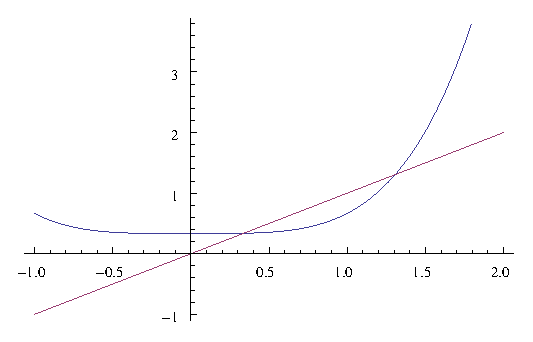
\includegraphics{Analysis/Analysis_1_1.eps}}
\end{figure}

\centertexdraw{
    
    \def\bdot {\fcir f:0 r:0.03 }
    
    \drawdim in

    \arrowheadtype t:F \arrowheadsize l:0.08 w:0.04
    \linewd 0.01 \setgray 0 

    \move (-1 -1) \lvec(2 2)
    \move (-1 0) \clvec (1 0.5)(1.5 1)(2 1.5)
  
    \move (-1 -1) \avec (-1 0 ) \avec(0 0) \avec(0 0.3) \avec(0.3 0.3) \avec(0.3 0.4)
    \move (2 2) \avec (2 1.5) \avec(1.5 1.5) \avec(1.5 1.05) \avec(1.05 1.05) \avec(1.05 0.75) \avec(0.75 0.75) \avec(0.75 0.6)\avec(0.6 0.6)
    
    \move (0.46 0.46) \bdot   
    \htext (-1.1 -1){0}
    \htext (0.4 0.2){$r_1$}

    \move (2 -1) \lvec(5 2)
    \move (2.2 -1) \clvec (3.2 0.5)(3.4 1)(3.7 2)

    \move (2.57 -0.43) \bdot   
    \move (3 0) \avec (3 0.3) \avec (3.3 0.3) \avec (3.3 0.85) \avec (3.85 0.85) \avec (3.85 2) 
    \htext (2.8 -0.5){$r_2$}
 
\move (0 -1.2)
}

Let the two roots of $f(x) = (x^4+1)/3 - x$ be $r_1$ and $r_2$ ($r_1 < r_2$). Because $f(0)>0$, $f(1) <0$ and $f(2) >0$, we have $r_1 \in (0,1)$ and $r_2\in (1,2)$.

Graphical analysis tells us that sequences starting with $a_1 =0,1$ converge to $r_1$ and $a_1 = 2$ diverges to infinity.

$a_1 = 0$. If $a_n \in (0,r_1)$, $f(a_n) = (a_n^4+1)/3 - a_n = a_{n+1} -a_n >0\ \ra \ a_{n+1} > a_n$. But
\be
a_{n+1} = (a_n^4+1)/3 < (r_1^4+1)/3 = r_1   
\ee

Thus, $a_n$ is increasing and bounded above so it is converging.

$a_1 = 1$. If $a_n \in (r_1,r_2)$, $f(a_n) = (a_n^4+1)/3 - a_n = a_{n+1} -a_n < 0\ \ra \ a_{n+1} < a_n$. But
\be
a_{n+1} = (a_n^4+1)/3 > (r_1^4+1)/3 = r_1   
\ee

Thus, $a_n$ is decreasing and bounded above so it is converging.

$a_1 = 2$. If $a_n \in (r_2,\infty)$, $f(a_n) = (a_n^4+1)/3 - a_n = a_{n+1} -a_n >0\ \ra \ a_{n+1} > a_n$. Thus, $a_n$ is increasing and unbounded above so it is diverging.

\vspace{2mm}

------------------------------------------------------------------------------------------------------------------

\begin{exercise}
Let $a_1>b_1>0$ and let $a_{n+1} = (a_n + b_n)/2$, $b_{n+1} = 2a_nb_n/(a_n+b_n)$ for $n\geq 1$. Show that $a_n>a_{n+1}>b_{n+1}>b_n$ and deduce the two sequences converge to a common limit. What limit?
\end{exercise}

Solution. Since $a_1>b_1>0$,
\be
\left\{\ba{l}
2a_1 > a_1 + b_1 \ \ra \ a_1 > \frac{a_1 + b_1}2 = a_2\\
\frac 1{a_1} < \frac 1{b_1} \ \ra \  \frac 1{a_1} + \frac 1{b_1}  < \frac 2{b_1} \ \ra \ b_1 < \frac 2{\frac 1{a_1} + \frac 1{b_1}} = b_2\\
a_2 - b_2 = \frac{a_1 + b_1}2 - \frac {2a_1b_1}{a_1 + b_1} = \frac {(a_1 - b_1)^2}{2(a_1+b_1)} >0
\ea\right. \ \ra \ a_1 > a_2 > b_2 > b_1.
\ee

By induction, we have $a_n>a_{n+1}>b_{n+1}>b_n$. Since $a_n$ is a decreasing sequence, and bounded below (by 0), thus $a_n$ converges to $a$. Similarly, $b_n$ is an increasing sequence and bounded above (by $a_1$). Thus,
\be
\left\{\ba{l}
a = \frac {a+b}2 \\
b = \frac {2ab}{a+b}
\ea\right. \ \ra \ a = b.
\ee
which means that $a_n$ and $b_n$ converge to a common limit $c$. We know that
\be
a_{n+1}b_{n+1} = (a_n + b_n)/2 \times 2a_nb_n/(a_n+b_n) = a_n b_n \ \ra \ c^2 = a_1 b_1 \ \ra \ c = \sqrt{a_1b_1}.
\ee

\begin{exercise}
Let $[a_n,b_n], \ n=1,2,\dots$ be closed intervals with $[a_n,b_n]\cap[a_m,b_m]\neq \emptyset$ for all $n,m$. Prove that $\cap^\infty_{n=1}[a_n,b_n]\neq \emptyset$.
\end{exercise}

Solution. First, we can not use induction to prove the statements about infinity! For example, consider the sets $A_n = [n,\infty),n\in \N$. We have
\be
\bigcap^k_{n=1} A_n = A_k \neq \emptyset = \bigcap^\infty_{n=1}A_n.
\ee

\begin{exercise}
The real sequence $a_n$ is bounded but does not converge. Prove that it has two convergent subsequences with different limits.
\end{exercise}

Solution. By Balzano-Weierstrass Theorem, $a_n$ is real and bounded, so $a_n$ contains a convergent subsequence. Let its limit be $l$. Because $a_n$ is not convergent, there exist $\ve>0$ s.t. there exists infinityly many terms of $a_n$ which satisfy 
\be
\abs{a_n -l} > \ve.
\ee
Now apply Balzano-Weierstrass Theorem again for these $a_n$. There exists another subsequence converges to another limit $m \neq l$. Thus, this real sequence $a_n$ has two convergent subsequences with different limits.

\begin{exercise}
Investigate the convergence of the following series. For those expressions containing the complex number $z$, find those $z$ for which convergence occurs.
\be
\sum_n\frac{\sin n}{n^2}\quad \quad \sum_n\frac{n^2z^n}{5^n}\quad\quad \sum_n\frac{(-1)^n}{4+\sqrt{n}}\quad\quad \sum_n \frac{z^n(1-z)}{n}
\ee
\end{exercise}

Solution. \ben
\item [(i)] It's obvious that $\abs{\frac {\sin n}{n^2}} \leq \frac 1{n^2}$ and $\sum_n \frac 1{n^2}$ converges. By comparison test, $\sum_n\frac{\sin n}{n^2}$ is absolutely convergent.

\item [(ii)] Using ratio test, we check
\be
\abs{\frac {a_{n+1}}{a_n}} = \abs{\frac{z(n+1)^2}{5n^2}} \to \abs{\frac z5}  \quad \text{as }n \to \infty.
\ee

Thus, we have
\be
\sum_n\frac{n^2z^n}{5^n}\quad
\left\{\ba{ll}
\text{converges absolutely }\quad \quad & \abs{z}<5\\
\text{inconclusive} & \abs{z} = 5\\
\text{diverges} & \abs{z} >5
\ea\right..
\ee

\item [(iii)] We know that $\frac 1{4+\sqrt{n}}$ is decreasing. Thus, by alternative test, $\sum_n\frac{(-1)^n}{4+\sqrt{n}}$ converges.

\item [(iv)] Use ratio test again, 
\be
\abs{\frac {a_{n+1}}{a_n}} = \abs{\frac{zn}{n+1}} \to \abs{z}  \quad \text{as }n \to \infty.
\ee
Thus, we have
\be
\sum_n \frac{z^n(1-z)}{n}\quad
\left\{\ba{ll}
\text{converges absolutely }\quad \quad & \abs{z}<1\\
\text{inconclusive} & \abs{z} = 1\\
\text{diverges} & \abs{z} >1
\ea\right..
\ee

\een

\begin{exercise}
Show that $\sum 1/(n\log^\alpha n)$ converges if $\alpha>1$ and diverges otherwise. Does $\sum 1/(n\log n\log\log n)$ converge?
\end{exercise}

Solution. Cauchy's condensation test. $a_n$ is decreasing sequence of positive terms, then $\sum^\infty_{n=1}a_n$ converges iff $\sum^\infty_{n=1}2^n a_{2^n}$ converges.

We know that $\frac 1{n\log^\alpha n}$ is decreasing. Using Cauchy' condensation test, we have
\be
\sum \frac 1{n\log^\alpha n} \text{ converges } \ \lra \ \sum \frac {2^n}{2^n\log^\alpha 2^n} \text{ converges } \ \lra \ \frac 1{\log^\alpha 2}\sum \frac {1}{n^\alpha } \text{ converges }
\ee

Thus $\sum_n \frac {1}{n^\alpha }$ converges iff $\alpha >1$, diverges otherwise.

For the decreasing sequence $\frac 1{n\log n\log\log n}$, we apply Cauchy's condensation test again,
\beast
\sum \frac 1{n\log n\log\log n} \text{ converges }& \lra & \sum \frac {2^n}{2^n\log 2^n\log\log 2^n} \text{ converges } \\
& \lra & \frac 1{\log 2}\sum \frac {1}{n\bb{\log n + \log\log 2}} \text{ converges }\\
& \lra & \sum \frac {2^n}{2^n\bb{n\log 2 + \log\log 2}} \text{ converges }\quad\quad \text{Cauchy's condensation test once more}\\
& \lra & \sum \frac {1}{n\log 2 + \log\log 2} \text{ converges }
\eeast

It's obvious that
\be
\frac {1}{n\log 2 + \log\log 2} \text{ diverges } \ \ra \ \sum \frac 1{n\log n\log\log n} \text{ diverges.}
\ee

\begin{exercise}
Let $a_n\in\C$ and let $b_n = \frac 1n\sum^n_{i=1}a_i$. Show that, if $a_n\to a$ as $n\to\infty$, then $b_n\to a$ also.
\end{exercise}

Solution. 

\begin{exercise}
Consider the two series $1-\frac 12 + \frac 13 - \frac 14+ \frac 15- \frac 16+\cdots$ and $1+ \frac 13 -\frac 12 + \frac 15 + \frac 17 - \frac 14+ \cdots$ having the same terms but taken in a different order. Let $s_n$ and $t_n$ be the corresponding partial sums to $n$ terms. Show that $s_{2n} = H_{2n}-H_n$ and $t_{3n} = H_{4n} - \frac 12H_{2n} -\frac 12H_{n}$, where $H_n = 1 + \frac 12 + \frac 13 + \frac 14 + \frac 15 + \cdots + \frac 1n$. Show that $s_n$ converges to a limit $s$ and that $t_n$ converges to $3s/2$.
\end{exercise}

Solution. We have
\beast
s_{2n} & = &  1 - \frac 12 + \frac 13 - \frac 14 \dots + \frac 1{2n-1} - \frac 1{2n}\\
& = & 1 + \frac 12 + \frac 13 + \frac 14 + \dots + \frac 1{2n-1} + \frac 1{2n} - 2\bb{\frac 12 + \frac 14 + \dots + \frac 1{2n}}\\
& = & H_{2n} - H_n.
\eeast

\beast
t_{3n} & = &  \bb{1 + \frac 13 - \frac 12 } + \bb{\frac 15 + \frac 17 - \frac 14 } + \bb{ \frac 1{4n-3} + \frac 1{4n-1}- \frac 1{2n}}\\
& = & \bb{1 + \frac 12 + \frac 13 + \frac 14 + \dots + \frac 1{4n-1} + \frac 1{4n}} - \bb{\frac 12 + \frac 14 + \dots + \frac 1{4n-2} + \frac 1{4n}} - \bb{\frac 12 + \frac 14 + \dots + \frac 1{2n}}\\
& = & H_{4n} - \frac 12 H_{2n} - \frac 12 H_n.
\eeast

Also,
\be
s_{n} \to 1 - \frac 12 + \frac 13 - \frac 14 \dots + \dots = \sum \frac {(-1)^{n+1}}{n} = \log(1+1) = \log 2.
\ee

\beast
t_{n} & \to & \sum \bb{ \frac 1{4n-3} + \frac 1{4n-1}- \frac 1{2n}} \\
& = & \sum \bb{ \frac 1{4n-3} + \frac 1{4n-1}- \frac 1{4n-2} - \frac 1{4n}} +  \sum \bb{ \frac 1{4n-2} + \frac 1{4n}- \frac 1{2n}}\\
& = & \sum \frac {(-1)^{n+1}}{n} + \frac 12 \sum \frac {(-1)^{n+1}}{n} = \frac 32 \sum \frac {(-1)^{n+1}}{n} = \frac 32 \log 2.
\eeast

\begin{exercise}
Suppose that $\sum a_n$ diverges and $a_n>0$. Show that there exist $b_n$ with $b_n/a_n\to 0$ and $\sum b_n$ divergent.
\end{exercise}

Solution. Since $\sum a_n$ is increasing and divergent, we take a subsequence $N_k$ s.t. $N_0 = 0$, $N_1$ is the first integer where $\sum a_n$ crosses 1, similarly
\be
N_k = \inf\left\{n:\sum^n_{i=N_{k-1}+1}a_i \geq 1,\ n\in \N\right\}.
\ee

Then we define
\be
b_n := \frac {a_n}{k},\quad N_{k-1} < n \leq N_k
\ee
so that $b_n/a_n$ converges to 0 as $n\to \infty$. Also,
\be
\sum b_n = \sum^\infty_{k=1} \sum^{N_{k}}_{N_{k-1}+1} b_n = \sum^\infty_{k=1} \sum^{N_{k}}_{N_{k-1}+1} \frac {a_n}k = \sum^\infty_{k=1} \frac 1k \sum^{N_{k}}_{N_{k-1}+1}a_n \geq \sum^\infty_{k=1} \frac 1k = \infty.
\ee

Hence, $b_n$ is divergent.

\begin{exercise}[Abel's test]
Let $a_n$ and $b_n$ be two sequences and let $S_n=\sum^n_{j=1}a_j$ and $S_0=0$. Show that for any $1\leq m\leq n$ we have
\be
\sum^n_{j=m}a_jb_j = S_nb_n - S_{m-1}b_m + \sum^{n-1}_{j=m}S_j(b_j-b_{j+1}).
\ee
Suppose now that $b_n$ is a decreasing sequence of positive terms tending to zero. Moreover, suppose that $S_n$ is a bounded sequence. Prove that $\sum^\infty_{j=m}a_jb_j$ converges. Deduce the alternative series test. Does the series $\sum^\infty_{n=1}\frac{\cos(n)}{n}$ converge or diverge?
\end{exercise}

Solution. First, we have
\be
S_n b_n = a_1b_n + a_2b_n + \dots + a_nb_n,\quad \quad S_{m-1}b_m = a_1b_m + a_2b_m + \dots + a_{m-1}b_m
\ee
and
\be
\sum^{n-1}_{j=m}S_j(b_j-b_{j+1}) = (a_1 + a_2+ \dots + a_m)b_m + (a_{m+1}b_{m+1} + \dots + a_{n-1}b_{n-1}) - (a_1 + a_2 + \dots + a_{n-1})b_n
\ee

Thus, we sum these up to get
\be
S_nb_n - S_{m-1}b_m + \sum^{n-1}_{j=m}S_j(b_j-b_{j+1}) = a_m b_m + (a_{m+1}b_{m+1} + \dots + a_{n-1}b_{n-1}) + a_n b_n = \sum^n_{j=m}a_jb_j.
\ee

Also, we know that $S_n$ is bounded, $\abs{S_n} \leq k$ for some $k$ and $\forall n\in \N$
\beast
\abs{\sum^n_{j=m} a_j b_j} & \leq & \abs{S_nb_n} + \abs{S_{m-1}b_m} + \abs{\sum^{n-1}_{j=m}S_j(b_j-b_{j+1})}\\
& \leq & k b_n + k b_m + k \abs{b_m - b_{n-1}} = 2k b_m.
\eeast

Since $\lim_{m\to\infty}b_m = 0$, $2kb_m$ can be arbitrarily small so by Cauchy's criterion, $\abs{\sum^n_{j=1} a_j b_j}$ converges, so does $\abs{\sum^n_{j=m} a_j b_j}$.

Now let $a_n = (-1)^{n+1}$ then $S_n = 0 \text{ or }1$ which is bounded. Then by Abel's test, the alternative series test holds. 

For the series $\sum^\infty_{n=1}\frac{\cos(n)}{n}$, we have $b_n = \frac 1n$, and 
\be
\sum^n_{k=1} a_k = \sum^n_{k=1} \cos k = \Re\bb{\sum^n_{k=1} e^{ki}} = \Re\bb{\frac{e^{(n+1)i}-1}{e^i - 1}}
\ee
is bounded. Thus, with Abel's test, we know that the series converges.

\begin{exercise}
For $n\geq 1$, let 
\be
a_n = \frac 1{\sqrt{n}} + \frac{(-1)^{n-1}}{n}.
\ee
Show that each $a_n$ is positive and that $\lim a_n =0$. Show also that $\sum^\infty_{n=1}(-1)^{n-1}a_n$ diverges. [This shows that, in the alternative series test, it is essential that the moduli of the terms decrease as $n$ increases.]
\end{exercise}

Solution. Since $n\geq 1$, $\frac 1{\sqrt{n}}\geq \frac 1n$. Thus, we have $a_n \geq 0$. Also,
\be
\lim_{n\to\infty}a_n = \lim_{n\to\infty}\frac 1{\sqrt{n}} + \lim_{n\to\infty}\frac{(-1)^{n-1}}{n} = 0 + 0 = 0.
\ee

Assume $\sum^\infty_{n=1}(-1)^{n-1}a_n$ converges, we have
\be
\sum^\infty_{n=1}(-1)^{n-1}a_n = \sum^\infty_{n=1}(-1)^{n-1}\frac 1{\sqrt{n}} + \sum^\infty_{n=1}\frac 1n.
\ee
The first part converges by alternative test and second part diverges. Hence, this contradiction gives the divergence of the series.

\begin{exercise}
Let $z\in \C$. Show that the series
\be
\frac{z}{1-z^2} + \frac{z^2}{1-z^4} + \frac{z^4}{1-z^8} + \frac{z^8}{1-z^{16}} + \cdots
\ee
converges to $z/(1-z)$ if $|z|<1$, converges to $1/(1-z)$ if $|z|>1$, and diverges if $|z|=1$.
\end{exercise}

Solution. Let $S_n$ be the partial sum of the $n$th partial sum and assume
\be
S_n = \frac 1{1-z} - \frac 1{1-z^{2^n}}.
\ee

Thus,
\be
S_1 = \frac 1{1-z} - \frac 1{1-z^{2}} = \frac z{1-z^2}
\ee
holds. Then by induction, 
\be
S_k = \frac 1{1-z} - \frac 1{1-z^{2^k}}  \ \ra \ S_{k+1} =  \frac 1{1-z} - \frac 1{1-z^{2^k}} + \frac {z^{2^k}}{1-z^{2^{k+1}}} = \frac 1{1-z} - \frac 1{1-z^{2^{k+1}}}. 
\ee
So $S_n$ is true for all $n\in \N$.

If $|z|<1$, as $n\to\infty$, $z^{2^n} \to 0$, thus $S_n \to \frac 1{1-z}-1 = \frac z{1-z}$ as $n\to\infty$.

If $|z|>1$, $\frac 1{|z^{2^n}|}\to 0$ as $n\to\infty$, so $\frac 1{1-z^{2^n}}\to 0$ and $S_n \to \frac 1{1-z}$ as $n\to\infty$.

If $|z|=1$, $S_n$ converges iff $\frac 1{1-z^{2^n}}\to 0$. We have
\be
\abs{\frac 1{1-z^{2^n}}-0} = \abs{\frac 1{1-z^{2^n}}} = \frac 1{\abs{1-z^{2^n}}} \geq \frac 1{1+\abs{z^{2^n}}} = \frac 12 \neq 0
\ee
Thus, we can say that $S_n$ diverges.

\begin{exercise}
Prove that every real sequence has a monotonic subsequence. Deduce the Bolzano-Weierstrass theorem. Show that the Bolzano-Weierstrass theorem is in fact equivalent to the fundamental axim, that is, give a proof of the fundamental axiom assuming Bolzano-Weierstrass.
\end{exercise}

Solution. Let $\{x_n\}$ be a real sequence. Let's call $x_N$ a 'peak' point if $x_N\geq x_i,\ \forall i >N$. 
\ben
\item [(i)] If there are inifinitely many 'peak' points, then these 'peak' points can form a monotonically decreasing subsequence.
\item [(ii)] If there are only finitely many 'peak' ponts, let them be $x_{N_1},x_{N_2},\dots,x_{N_k}$. Pick $m_1>N_k$, then there exists $m_2>m_10$ s.t. $x_{m_2} > x_{m_1}$ (since $x_{m_1}$ is not a 'peak' point). Again pick $m_3>m_2$ s.t. $x_{m_3} > x_{m_2}$. Continuing this procedure, we have a sequence $x_{m_i},\ i \in \N$ which is a monotonically increasing subsequence.
\een
Thus, every real sequence has a monotonic subsequence.

\vspace{4mm}

{\bf The Bolzano-Weierstrass Theorem}. If $x_n\in\mathbb{R}$ and there exists $K$ s.t. $|x_n|<K,\forall n$, then we can find $n_1<n_2<\dots$ and $x\in\mathbb{R}$ s.t. $x_{n_j}\to x$ as $j\to \infty$. (every bounded sequence has a convergent subsequence.)

{\bf Proof}. We see $[a_n,b_n] = [-K,K]$, let $c=\frac{a_0+b_0}{2}$ (mid-point), thus, either
\ben
\item [(i)] $x_n\in[a_0,c]$ for infinitely many values of $n$;
\item [(ii)] $x_n\in[c,b_0]$ for infinitely many values of $n$.
\een

In case (i), set $a_1=a_0, b_1=c$; 

In case (ii), set $a_1=c,b_1=b_0$. 

Proceed inductively to obtain sequences $a_n$ and $b_n$ s.t. the following holds ($m\leq n$)
\ben
\item [(i)] $a_m\leq a_n\leq b_n\leq b_m$; ($a_n$ is a bounded increasing sequence, $b_n$ is a bounded decreasing sequence.)
\item [(ii)] $x_m\in[a_n,b_n]$ for infinitely many values of $m$;
\item [(iii)] $b_n-a_n=\frac{b_{n-1}-a_{n-1}}{2}$.
\een

By the Fundamental Axiom, $a_n\to a$ and $b_n\to b$. By property (iii) passing to the limit,
\begin{equation*}
b-a = \frac{b-a}{2}\ \Rightarrow \ a=b
\end{equation*}

Having selecting $n_j$ s.t. $x_{n_j}\in[a_j,b_j]$, select $n_{j+1}>n_j$ s.t. $x_{n_{j+1}}\in[a_{j+1},b_{j+1}]$, we can always do this because $x_m\in[a_{j+1},b_{j+1}]$ for infinitely many values of $m$. In other words, 
\be
\left\{\ba{c}
a_j\leq x_{n_j} \leq b_j, \forall j\\
\\
a_j\to a,\ b_j\to b=a
\ea\right.\ \Rightarrow \ x_{n_j}\to a. \quad\quad \fbox{}
\ee

\begin{exercise}
Can we write the open interval $(0,1)$ as a disjoint union of closed intervals of positive length?
\end{exercise}

Solution. 

\vspace{2mm}

------------------------------------------------------------------------------------------------------------------

\begin{exercise}
Is there an enumeration of $\Q$ as $q_1,q_2,q_3,\dots$ such that $\sum(q_n-q_{n+1})^2$ converges?
\end{exercise}

Solution. 

%%%%%%%%%%%%%%%%%%%%%%%%%%%%%%%%%%%%%%%%%%%%%%%%%%%%

\begin{exercise}
Define $f : \R \to \R$ by $f(x) = x$ if $x \in \Q$ and $f(x) = 1-x$ otherwise. Find $\{a : f \text{ is continuous at }a\}$.
\end{exercise}

Solution. $\forall \ve >0$, let $\delta = \ve$. Then for $x$ s.t. $\abs{x-\frac 12} < \delta$, 
\be
\abs{f(x)-f\bb{\frac 12}} = \left\{\ba{ll}
\abs{x-\frac 12} < \delta = \ve & \text{if }x\in \Q\\
\abs{1-x-\frac 12} = \abs{x-\frac 12}  < \delta = \ve  \quad\quad & \text{if }x\in \R\backslash\Q
\ea\right.
\ee
Thus $f(x)$ is continuous at $\frac 12$.



\emph{Approach 1}. Now if $f(x)$ is also continuous at $a>\frac 12$. Let $a=\frac 12 + \ve$, $\ve >0$ and $x,y >a$, $\exists \delta >0$ 
\be
\abs{x-a} < \delta, \ x \in \Q,\quad\quad \abs{y-a} < \delta, \ y \in \R\backslash\Q
\ee
such that
\be
\abs{f(x)-f(a)} < \ve,\quad \abs{f(y)-f(a)} < \ve \ \ra \ \abs{f(x)-f(y)} < 2\ve.
\ee

However,
\be
\abs{f(x)-f(y)} = \abs{x+y-1} = x+y-1 > 2a-1 = 2\bb{\frac 12+\ve} -1 = 2\ve \ \ra \ \text{Contradiction.}
\ee

\emph{Approach 2}. If $f(x)$ is continuous at $a\neq \frac 12$, then for any sequence $x_n \to a$, $f(x_n)\to f(a)$. Thus, we pick the sequence $y_n \in \R\backslash\Q$ s.t. $y_n \to a$, then $f(y_n) \to a$.
\be
a =  \lim_{n\to \infty}f(y_n) =  \lim_{n\to \infty}1-y_n = 1 -  \lim_{n\to \infty}y_n = 1-a \ \ra \ a = \frac 12. \quad \text{Contradiction.}
\ee

Hence, $f(x)$ is only continuous at $\frac 12$.

\begin{exercise}
Write down the definition of "$f(x) \to \infty$ as $x \to \infty$". Prove that $f(x) \to \infty$ as $x \to\infty$ if, and only if, $f(x_n) \to \infty$ for every sequence such that $x_n \to\infty$.
\end{exercise}

Solution. Definition. $f(x) \to \infty$ as $x \to \infty$ if $\forall \ve >0$, $\exists \delta >0$ s.t. $\forall x> \delta$, $f(x)>\ve$.

Proof. '$\Longrightarrow$'.
\beast
\left\{\ba {l}
f(x) \to \infty \text{ as }x \to \infty \ \ra \ \forall \ve >0,\ \exists \delta >0 \text{ s.t. }\forall x> \delta,\ f(x)>\ve\\
x_n \to \infty \ra \forall \delta >0,\ \exists N>0 \text{ s.t. } \forall n\geq N,\ x_n > \delta
\ea\right.\quad\quad\quad\quad\quad\quad\quad\quad\quad\quad\quad\quad\quad\quad\quad\quad\quad\quad\\
\ra
\left\{\ba{l}
\forall \ve >0,\ \exists N >0 \text{ s.t. }\forall n \geq N,\ f(x_n)>\ve\\
\text{ which means }f(x_n) \to \infty.
\ea\right.
\eeast

'$\Longleftarrow$'. We have
\be
f(x) \nrightarrow \infty \text{ as }x \to \infty\ \ra \ \forall \delta >0,\ \exists \ve>0 \text{ s.t. }\exists x > \delta,\ f(x)<\ve.
\ee

Choose $\delta_n = n$, thus there is a sequence $x_n > \delta_n$, so $x_n \to \infty$. As $n=\delta_n \to\infty$,
\be
\exists \ve>0, n>0, \ f(x_n) <\ve\ \ra \ f(x_n) \nrightarrow \infty.
\ee
%
%\beast
%\left\{\ba {l}
%f(x) \nrightarrow \infty \text{ as }x \to \infty\ \ra \ \forall \delta >0,\ \exists \ve>0 \text{ s.t. }\exists x > \delta,\ f(x)<\ve\\
%x_n \to \infty \ra \forall \delta >0,\ \exists N>0 \text{ s.t. } \forall n\geq N,\ x_n > \delta
%\ea\right. \quad\quad\quad\quad\quad\quad\quad\quad\quad\quad\quad\quad\\
%\\
% \ra 
%\forall \delta >0,\ \exists \ve>0, N>0 \text{ s.t. }\exists n \geq N, x_n > \delta,\ f(x_n)<\ve\quad\quad\quad\quad\quad\quad\quad\quad\\
%\\
% \ra \left\{\ba{l}
%\forall N>0,\ \exists \ve>0, n\geq N \text{ s.t. } \ f(x_n)<\ve \\
%\text{ which means }f(x_n) \nrightarrow \infty.
%\ea\right.
%\eeast

\begin{exercise}
Suppose that $f(x) \to l$ as $x \to a$ and $g(y) \to k$ as $y \to l$. Must it be true that $g(f(x)) \to k$ as $x \to a$?
\end{exercise}

Solution. No. If $f(x)$ is continuous at $a$ and $g(y)$ is not continuous at $l$, let's say
\be
f(x) = 2,\quad\quad g(y) = \left\{\ba{ll}
1 \quad\quad & y \neq 2\\
3 & y = 2
\ea\right.
\ee
which means that $l = 2$, $k=1$. However,
\be
g(f(x)) \to g(2) = 3 \neq 1 \ (k) \quad\quad \text{as }x\to a.
\ee

\begin{exercise}
Let $f_n : [0, 1] \to [0, 1]$ be continuous, $n \in \N$. Let $h_n(x) = \max\{f_1(x), f_2(x), \dots, f_n(x)\}$. Show that $h_n$ is continuous on $[0, 1]$ for each $n \in \N$. Must $h(x) = \sup\{f_n(x) : n \in \N\}$ be continuous?
\end{exercise}

Solution. Realizing for two continuous functions $f$ and $g$
\be
\max\{f,g\} = \frac{(f+g)+\abs{f-g}}2
\ee

We have $f+g$ and $abs{f-g}$ as continuous functions as well. Thus, $\max\{f,g\}$ is continuous. Also, we know that

\be
\max\{f_1(x), f_2(x), \dots, f_n(x)\} = \max\{f_1(x),\max\{f_2(x),\dots,f_n(x) \}\}.
\ee

By induction, we have that $h_n(x)$ is continuous.

Now consider $f_n(x) = \min\{nx,1\},\ x\in[0,1]$. Obviously, $f_n(x)$ is continuous. For any $x\in(0,1]$, there exists $N\in \N$ s.t. $Nx > 1$. Thus, $\forall n\geq N$, $f_n(x) = 1$. This implies that 
\be
h(x) = \sup\{f_n(x) : n \in \N\} = 1,\quad x\in (0,1].
\ee

Then consider $x=0$, we have $f_n(x) = 0$ for all $n$. Hence we have
\be
h(x) = \left\{\ba{ll}
1 \quad\quad & x\neq 0\\
0 & x= 0
\ea\right.
\ee
which is NOT continuous on $[0,1]$.

\begin{exercise}
The unit circle in $\C$ is mapped to $\R$ by a map $e^{i\theta} \mapsto f(\theta)$, where $f : [0, 2\pi] \to \R$ is continuous and $f(0) = f(2\pi)$. Show that there exist two diametrically opposite points that have the same image.
\end{exercise}

Solution. Consider $g(x) = f(x+\pi)-f(x)$, $x\in [0,\pi]$. Then we have three cases:
\ben
\item [(i)] If $f(0) = f(\pi)$, 0 and $\pi$ are diametrically oppositte points, done.
\item [(ii)] If $f(0) > f(\pi)$, 
\be
g(0) = f(\pi) -f(0) < 0, \quad g(\pi) = f(2\pi) - f(\pi) = f(0) - f(\pi) > 0.
\ee
By I.V.T., $\exists x^* $ such that $g(x^*) = 0$ which implies that $f(x^*+\pi) = f(x^*)$.
\item [(iii)] If $f(0) < f(\pi)$, use the same argument.
\een

\begin{exercise}
Let $f(x) = \sin^2 x + \sin^2(x + \cos^7 x)$. Assuming the familiar features of $\sin$ without justification, prove that there exists $k > 0$ such that $f(x) \geq k$ for all $x \in \R$.
\end{exercise}

Solution. First, we have $f(x)$ is non-negative and continuous on $[0,2\pi]$. Thus, there exists $k \geq 0$ such that $f(x)\geq k$. If $f(x) = 0$, we have 
\be
\left\{\ba{l}
\sin^2 x = 0\\
\sin^2(x + \cos^7 x) = 0
\ea\right. \ \ra \ 
\left\{\ba{l}
x = k\pi,\ k\in \Z \\
x + \cos^7 x = m\pi,\ m\in \Z
\ea\right. \ \ra \ \cos^7 x = (m-k)\pi
\ee
which gives
\beast
 -1\leq (m-k)\pi\leq 1 & \ra & k-\frac 1{\pi} \leq m \leq k+ \frac 1{\pi} \\
& \ra &  m=k \ \ra \ \cos^7x = 0 \ \ra \ \cos x = 0 \ \ra \ x = n\pi + \frac {\pi}2, \ n\in\Z \quad \text{contradiction}.
\eeast
Thus, there is no $x$ satisfying $f(x) = 0$ and $f(x) >0$. So $k$ can not be 0, then we have $k>0$.

\begin{exercise}
Suppose that $f : [0, 1] \to \R$ is continuous, that $f(0) = f(1) = 0$, and that for every $x \in (0, 1)$ there exists $0 < \delta < \min\{x, 1 - x\}$ with $f(x) = (f(x - \delta) + f(x + \delta))/2$. Show that $f(x) = 0$ for all $x$.
\end{exercise}

Solution. Since $f:[0,1]\mapsto \R$ is continuous, $\exists K$ s.t. $f(x)\leq K$ and $K$ can be achieved. ($K\geq 0$)

Let $S =\{x:f(x) = K, x\in [0,1]\}$. Since $S$ is bounded below (by zero), $\inf S$ exists. Let $r= \inf S$. By definition of infimum, $\exists x_n \in [0,1]$ s.t. 
\be
r+\frac 1n \geq x_n \geq r,\quad \quad f(x_n) = K.
\ee

By Bolzano-Weierstrass Theorem, $\exists x_{n_j} \to a$ as $j\to \infty$, thus
\be
r \leq x_{n_j} \leq r+ \frac1{n_j} \to r \text{ as }j\to \infty\ \ra \ r=a \ \ra \ \lim_{j}f(x_{n_j}) = f(a) =f(r) = K.
\ee

If $0<r<1$, $f(r-\delta) <K$ (since $r$ is infimum of $S$), we have
\be
f(x) = (f(x - \delta) + f(x + \delta))/2 \ \ra \ f(r) = (f(r - \delta) + f(r + \delta))/2 \ \ra \ f(r+\delta) > K.
\ee
This contradiction gives $r=0$, so $K = 0$. 

Similarly, $\exists L$ s.t. $f(x)\geq L$ and $L$ can be achieved. ($L\leq 0$). Using the same argument, we have $K=L=0$ which means that $f(x)=0$ for all $x$.

\begin{exercise}
Let $f : [a, b] \to \R$ be bounded. Suppose that $f((x + y)/2) \leq (f(x) + f(y))/2$ for all $x, y \in [a, b]$. Prove that $f$ is continuous on $(a, b)$. Must it be continuous at $a$ and $b$ too?
\end{exercise}

Solution. For $x\in (a,b)$, we consider $x,x+h,x+2h,\dots$. With the given inequality, we have
\beast
2f(x+h) \leq f(x) + f(x+2h) & \ra & 2\bb{f(x+h)-f(x)} \leq f(x+2h)-f(x) \\
& \ra & 2^k\bb{f(x+h)-f(x)} \leq f(x+2^k h)-f(x)
\eeast

We require that
\be
a \leq x+ 2^k h \leq b \ \ra \ h \leq 2^{-k}\min\{\abs{x-a},\abs{x-b}\}.
\ee

Also, we know that $f(x)$ is bounded, thus, $\exists M \geq 0$ such that
\be
\abs{f(x)} \leq M, \quad f(y)-f(x)\leq 2M, \ \forall x,y \in (a,b)
\ee

Thus, $\forall \ve >0$, if $f(x+h)-f(x) \geq \ve$, we have
\be
2^k\ve \leq 2^k\bb{f(x+h)-f(x)} \leq f(x+2^k h)-f(x) \ \ra \ f(x+2^k h)-f(x) \geq 2^k\ve
\ee

If we pick $k$ s.t.
\be
2^k\ve > 2M \ \bb{\text{i.e. }2^{-k} < \frac{\ve}{2M}},
\ee
then this is a contradiction for the bounded condition then implies $f(x+h)-f(x) < \ve$. So $\forall \ve>0$, we can have $f(x+h)-f(x) < \ve$ by choosing
\be
h \leq 2^{-k}\min\{\abs{x-a},\abs{x-b}\} < \frac{\ve}{2M} \min\{\abs{x-a},\abs{x-b}\}.
\ee

Hence, $f(x)$ is continuous on $(a,b)$. 

Now consider the case
\be
f(x) = \left\{\ba{ll}
1 \quad\quad & x=a,b\\
0 & x\in (a,b)
\ea\right.
\ee
The inequality 
\be
f((x + y)/2) \leq (f(x) + f(y))/2, \ \forall x, y \in [a, b]
\ee
is satisfied but $f(x)$ is NOT continuous at $a$ and $b$.

\begin{exercise}
Prove that $2x^5 +3x^4 +2x +16 = 0$ has no real solutions outside $[-2,-1]$ and exactly one inside.
\end{exercise}

Solution. First we have
\be
f(-1) = 15,\quad f(-2) = -4.
\ee

With I.V.T., $\exists c \in [-2,-1]$ s.t. $f(c) = 0$. Also, we have
\be
f'(x) = 10x^4+ 12x^3 + 2 = 2x^3(5x+6) + 2 =  2(x+1)(5x^3+x^2-x+1).% 10x^3 (x+1) + 2x^3 + 2=
\ee

Let $g(x) = 5x^3+x^2-x+1$. Thus,
\be
g'(x) = 15x^2 +2x -1 \ \ra g'(x) > 0, \ x \leq -1
\ee

With $g(-1) = -2$, we have $g(x) <0$, $x\leq -1$. Thus,
\be
f'(x) = 2(x+1)g(x) \geq 0,\ x\leq -1.
\ee

Hence, there is only one solution in $[-2,-1]$ and no solution in $(-\infty,-2]$. Furthermore, for $x\geq -1$, 
\be
f(x) = 2x^5 +3x^4 +2x +16 \geq -2 + 0 + -2 + 16 = 12 > 0.
\ee
Thus, there is no solution outline $[-2,-1]$.

\begin{exercise}
Let $f : [a, b] \to \R$ be continuous on $[a, b]$ and differentiable on $(a, b)$. Which of (1)-(4) must be true?
\ben
\item [(1)] If $f$ is increasing then $f'(x) \geq 0$ for all $x \in (a, b)$.
\item [(2)] If $f'(x) \geq 0$ for all $x \in (a, b)$ then $f$ is increasing.
\item [(3)] If $f$ is strictly increasing then $f'(x) > 0$ for all $x \in (a, b)$.
\item [(4)] If $f'(x) > 0$ for all $x \in (a, b)$ then $f$ is strictly increasing.
\een
[Increasing means $f(x) \leq f(y)$ if $x < y$, and strictly increasing means $f(x) < f(y)$ if $x < y$.]
\end{exercise}

Solution. \ben
\item [(1)] True. $\forall x\in(a,b)$, 
\be
f'(x) = \lim_{h\to 0} \frac{f(x+h)-f(x)}{h}
\ee
since
\be
\forall h>0,\ \frac{f(x+h)-f(x)}{h} \geq 0 \quad \text{(definition of increasing function)}
\ee
Thus,
\be
\lim_{h\to 0} \frac{f(x+h)-f(x)}{h} \geq 0 \ \ra \ f'(x) \geq, \ \forall x\in(a,b).
\ee
\item [(2)] True. Let $x,y\in [a,b]$ with $x<y$. The mean value theorem says 
\be
f(y)-f(x) = f'(c)(y-x), \quad \exists c\in (x,y).
\ee

Then $f'(c)\geq 0 \ \Rightarrow \ f(y)-f(x) = f'(c)(y-x) \geq 0 \ \ra \ f(y) \geq f(x)  \ra f(x) \text{ is increasing}$.

\item [(3)] False. Let $f(x) = x^3,\ x\in[-1,1]$. $f(x)$ is strictly increasing, but $f'(0) = 0$.
\item [(4)] True. Similar argument with (1).
\een

\begin{exercise}
Let $f : \R \to \R$ be differentiable for all $x$. Prove that if $f'(x) \to l$ as $x \to \infty$ then $f(x)/x \to l$. If $f(x)/x \to l$ as $x \to \infty$, must $f'(x)$ tend to a limit?
\end{exercise}

Solution. Without loss of generality, we assume $l=0$, since
\be
g(x) = f(x) - lx \ \ra\ g'(x) = f'(x) -l,\quad \frac{g(x)}{x} = \frac{f(x)}{x} -l.
\ee

With condition provided, we get $\forall \ve >0$, $\exists K >0$ s.t. 
\be
\abs{g'(x)} < \ve,\quad \forall x \geq K.
\ee

Now for any $y<x$,
\be
\abs{\frac{g(x)}{x}} \leq \abs{\frac{g(x)-g(y)}{x}} + \abs{\frac{g(y)}{x}}
\ee

Thus, $\forall \ve>0$, 
\be
\abs{\frac{g(x)-g(y)}{x}} \leq \abs{\frac{g(x)-g(y)}{x-y}} = \abs{g'(x^*)},\ x^*\in (y,x)\quad \bb{\text{by M.V.T. since $g(x)$ is differentiable}}
\ee
So $\exists K_1 >0$ s.t. 
\be
\abs{g'(x^*)} < \frac{\ve}2,\quad \forall x^* \geq K_1.
\ee

Also, $\exists K_2$ s.t.
\be
\abs{\frac{g(K_1)}{x}} < \frac {\ve}2, \quad \forall x\geq K_2
\ee

Thus, $\forall \ve>0$, $\exists K = \max\{K_1,K_2\}$ s.t.
\be
\abs{\frac{g(x)}{x}} \leq \abs{\frac{g(x)-g(K_1)}{x}} + \abs{\frac{g(K_1)}{x}} \leq \abs{g'(x^*)} + \abs{\frac{g(K_1)}{x}} < \frac{\ve}2 + \frac{\ve}2 = \ve, \quad \forall x\geq K.
\ee

It can be proved by L'H\^opital rule which is proved by using M.V.T..
\be
f(x)\to \infty,\ x \to \infty \ \ra \ \lim \frac{f'(x)}{x'} = \lim \frac{f(x)}{x} = l.
\ee

However, the inverse does not hold. For example, 
\be
f(x) = \sin x \ \ra \ \frac{f(x)}{x} = \frac{\sin x}{x} \to 0
\ee
but $f'(x) = \cos x$ does not converge.

\begin{exercise}
Let $f(x) = x + 2x^2 \sin(1/x)$ for $x \neq 0$ and $f(0) = 0$. Show that $f$ is differentiable everywhere and that $f'(0) = 1$, but that there is no interval around 0 on which $f$ is increasing.
\end{exercise}

Solution. For the function $f(x)$
\be
f'(x) = 1 + 4x\sin (1/x) - 2\cos(1/x),\quad x\neq 0
\ee
and
\be
f'(0) = \lim_{h\to 0} \frac{f(h)-f(0)}{h-0} = \lim_{h\to 0} \frac{f(h)}h = \lim_{h\to 0} \frac{h+ 2h^2 \sin(1/h)}{h} = 1+ 2\lim_{h\to 0}h \sin(1/h) = 1.
\ee

Thus, $f$ is differentiable everywhere. 

Now assume there is an interval around 0 on which $f$ is increasing. By the previous result, we have $f'(x)\geq 0$ for all $x$ on this interval.

However, $\forall \ve >0$, $\exists n$ s.t. $x = \frac 1{2n\pi} < \ve$ and
\be
f'(x) = 1 + 4x\sin (1/x) - 2\cos(1/x) = 1 + \frac2{n\pi} \sin (2n\pi) - 2\cos (2n\pi) = 1 -2 = -1 < 0.
\ee
The contradiction gives that there is no interval around 0 on which $f$ is increasing.

\begin{exercise}
Let $f :\R \to \R$ be a function which has the intermediate value property: If $f(a) < c < f(b)$, then $f(x) = c$ for some $x$ between $a$ and $b$. Suppose also that for every rational $r$, the set $S_r$ of all $x$ with $f(x) = r$ is closed, that is, if $x_n$ is any sequence in $S_r$ with $x_n \to a$, then $a \in S_r$. Prove that $f$ is continuous.
\end{exercise}

Solution. Proof by contradiction. Assume all the assumptions hold and $f(x)$ is NOT continuous at some points. That is saying there exists a convergent sequence $\{x_n\}$, $x_n \to a$ s.t. 
\be
\forall \delta >0, \ \exists \ve>0,\ \exists i \in \N \text{ s.t. } \abs{x_i -a}< \delta,\ \abs{f(x_i)-f(a)}>\ve.
\ee

Now without loss of generality, let $\{x_{n_j}\} =\{y_{j}\}$ be the subsequence s.t. $y_j<a$ satisfying the above condition. Then by the intermediate value property, $\forall k \in \N$, $\exists r \in (f(a),f(y_k))$ (or $(f(y_k),f(a))$) s.t. $f(z_k)=r$ for some $y_k < z_k < a$. 

Thus, we obtain a convergent sequence $\{z_k\}$ with $z_k \to a$ (since $y_k \to a$ and $y_k < z_k < a$). Also, $f(z_k) = r$, $\forall k\in\N$, $\lim_{k\to\infty}f(z_k) \neq f(a)$. Thus, $a\notin S_r$, so $S_r$ is not closed.

Hence, $f(x)$ must be continuous everywhere.

\begin{exercise}
Suppose that $f : \R \to \R$ satisfies $|f(x)-f(y)| \leq |x-y|^2$ for all $x, y \in \R$. Show that $f$ is constant.
\end{exercise}

Solution. Suppose $f$ is not constant. Take $a,b\in \R$ with $a<b$ and $f(a)\neq f(b)$, then choose $n\in\N$ with 
\be
n>\frac{(b-a)^2}{\abs{f(b)-f(a)}}
\ee
and for $i=0,1,\dots,n$ set 
\be
c_i = a + \frac in(b-a)
\ee
so that $c_0 = a$ and $c_n = b$. Then
\be
\abs{f(b)-f(a)} = \abs{f(c_n)- f(c_0)} \leq \sum^n_{i=1}\abs{f(c_i) -f(c_{i-1})} \leq \sum^n_{i=1}\abs{c_i - c_{i-1}}^2 = \sum^n_{i=1}\bb{\frac{b-a}n}^2 = \frac {(b-a)^2}n < \abs{f(b)-f(a)}.
\ee

The contradiction implies that $f$ must be constant. An alternative way to prove is to use $f'(x)$.

\begin{exercise}
Given $\alpha \in \R$, define $f_\alpha : [-1, 1] \to \R$ by $f_\alpha(x) = x^\alpha \sin(1/x)$ for $x \neq 0$ and $f_\alpha(0) = 0$. Is $f_0$
continuous? Is $f_1$ differentiable? Draw a table, with 4 columns labelled 0, 1, 2, 3 and with 6 rows labelled "$f_\alpha$ bounded", "$f_\alpha$ continuous2, "$f_\alpha$ differentiable", "$f'_\alpha$ bounded", "$f'_\alpha$ continuous", "$f'_\alpha$ differentiable". Place ticks and crosses at appropriate places in the table. 

Does $|x|^\alpha \sin(1/x)$ behave the same way? Complete 5 extra columns, for $\alpha = -\frac 12 , \frac 12 , \frac 32 , \frac 52 , \frac 72$.
\end{exercise}

Solution. The table is
\begin{center}
\begin{tabular}{l|ccccccccc}
 & \ $-\frac 12 $ \ & \ 0 \ & \ $\frac 12 $ \ & \ 1 \ & \ $\frac 32 $ \ & \ 2 \ & \ $\frac 52 $ \ & \ 3 \  & \ $\frac 72$ \ \\ \hline
$f_\alpha$ bounded & $\times$ & $\surd$ & $\surd$ & $\surd$ & $\surd$ & $\surd$ & $\surd$ & $\surd$ & $\surd$  \\ 
$f_\alpha$ continuous & $\times$ & $\times$ & $\surd$ & $\surd$ & $\surd$ & $\surd$ & $\surd$ & $\surd$ & $\surd$  \\ 
$f_\alpha$ differentiable & $\times$ & $\times$ & $\times$ & $\times$ & $\surd$ & $\surd$ & $\surd$ & $\surd$ & $\surd$  \\ 
$f_\alpha'$ bounded & $\times$ & $\times$ & $\times$ & $\times$ & $\times$ & $\surd$ & $\surd$ & $\surd$ & $\surd$  \\ 
$f_\alpha'$ continuous & $\times$ & $\times$ & $\times$ & $\times$ & $\times$ & $\times$ & $\surd$ & $\surd$ & $\surd$  \\ 
$f_\alpha$ differentiable & $\times$ & $\times$ & $\times$ & $\times$ & $\times$ & $\times$ & $\times$ & $\times$ & $\surd$  
\end{tabular}
\end{center}

Both functions behave in the same way for $\alpha\in\Z$. 
\beast
|x|^\alpha \sin(1/x)\text{ is bounded } & \lra & \alpha \geq 0,\\
|x|^\alpha \sin(1/x)\text{ is continuous } & \lra & \lim_{h\to 0} \abs{h}^\alpha \sin \frac 1h = 0 \lra \alpha >0, \\
|x|^\alpha \sin(1/x)\text{ is differentiable} & \lra & \lim_{h\to 0}\frac{\abs{h}^\alpha \sin \frac 1h}{h} \text{ exists} \lra \alpha >1. 
\eeast

Thus, we obtain the table shown.

\begin{exercise}
By applying the mean value theorem to $\log(1 + x)$ on $[0, a/n]$ with $n > |a|$, prove carefully that $(1 + a/n)^n \to e^a$ as $n \to \infty$.
\end{exercise}

Solution. Set $f(x) = \log (1+x)$ and fix $a\in\R$. If $a =0$, then
\be
\bb{1+\frac an}^n = 1 = e^0 = e^a, \ \forall n \in \N.
\ee

So we assume $a\neq 0$, given $n > |a|$, apply the M.V.T. to either $\bsb{0,\frac an}$ or $\bsb{\frac an, 0}$ according as $a>0$ or $a<0$, there exists $x\in \bb{0,\frac an}$ with 
\be
f'(x) = \frac{f\bb{\frac an}-0}{\frac an - 0} \quad \text{i.e.},\quad \frac 1{1+x} = \frac na \log \bb{1+\frac an}.
\ee

As $n\to \infty$, since $|x| < \frac {\abs{a}}n$ we have $x\to 0$, so
\be
\frac 1{1+x} \to 1 \ \ra \ \frac na \log \bb{1+\frac an} \to 1 \ \log \bb{1+\frac an}^n \to a.
\ee

Finally, as $\exp$ is continuous, 
\be
\bb{1 + \frac an}^n \to e^a.
\ee

\begin{exercise}
Find $\lim_{n\to\infty} n(a^{1/n} - 1)$, where $a > 0$.
\end{exercise}

Solution. Set $f(x) = a^x$ and apply the M.V.T. to $\bsb{0,\frac 1n}$, there exists $x\in \bb{0,\frac 1n}$ with
\be
f'(x) = \frac{f\bb{\frac 1n} - f(0)}{\frac 1n - 0} \ \ra \ a^x \log a = n\bb{a^{\frac 1n} - 1}.
\ee

As $n\to \infty$, we have $x\to 0$. Thus,
\be
\lim_{n\to \infty} n\bb{a^{\frac 1n} - 1} = \lim_{x\to 0} a^x \log a = \log a.
\ee

\begin{exercise}
"Let $f'$ exist on $(a, b)$ and let $c \in (a, b)$. If $c + h \in (a, b)$ then $(f(c + h) - f(c))/h = f'(c + \theta h)$. Let $h \to 0$; then $f'(c + \theta h) \to f'(c)$. Thus $f'$ is continuous at $c$." Is this argument correct?
\end{exercise}

Solution. The argument is NOT correct as it can be seen by taking 
\be
f(x) = x^2\sin \frac 1x, \ x\neq 0,\quad f(0) = 0 \ \ra \ f'(x) = 2x\sin \frac 1x - \cos \frac 1x.
\ee

Thus, $\lim_{h\to 0} f'(c+\theta h) \neq f'(c)$ because $f'(c)$ contains $\cos \frac 1c$. 

Although as $h\to 0$ the values $c+\theta h$ tend to $c$, the $\theta$ may vary, so one cannot conclude that for all sequences $(x_n)$ tending to $c$ we have $f'(x_n) \to f'(c)$.

\begin{exercise}
Let $f : \R \to \R$ be defined by $f(x) = \exp(-1/x^2)$ for $x \neq 0$ and $f(0) = 0$. Show that $f$ is continuous and differentiable. Show that $f$ is twice differentiable. Indeed, show that $f$ is infinitely differentiable, and that $f^{(n)}(0) = 0$ for all $n\in \N$. Comment, in the light of what you know about Taylor series.
\end{exercise}

Solution. We prove by induction that for all $n\in \N$ the function $f$ is $n$ times differentiable, with $f^{(n)}(0)=0$ and $f^{(n)}(x) = P_n\bb{\frac 1x}f(x)$ for $x\neq 0$, where $P_n$ is some polynomial. Since 
\be
f'(0) = \lim_{h\to 0} \frac{f(h)-f(0)}{h} = \lim_{h\to 0} \frac{e^{-\frac 1{h^2}}-f(0)}{h} = \lim_{y\to \infty} \frac{y}{e^{y^2}} = 0,
\ee
while for $x\neq 0$ we have
\be
f'(x) = \frac 2{x^3}e^{-1/x^2} = P_1\bb{\frac 1x} f(x),
\ee
where $P_1(t) = 2t^3$, thus the statement is true if $n=1$. (The differentiability implies the continuity.)

Proof. $f$ is differentiable at $x_0$, which implies
\be
\lim_{x\to x_0} = \frac{f(x)-f(x_0)}{x-x_0} = f'(x_0).
\ee

We want to prove that $\lim_{x\to x_0}f(x) = f(x_0)$.
\be
\lim_{x\to x_0} f(x)-f(x_0) = \lim_{x\to x_0} (x-x_0) \frac{f(x)-f(x_0)}{x-x_0} = \lim_{x\to x_0} (x-x_0) \lim_{x\to x_0}\frac{f(x)-f(x_0)}{x-x_0} = 0 \cdot f'(x_0) = 0.
\ee
Thus, $f$ is continuous at $x_0$.

Now assume it is true for $n=k$, then 
\be
f^{(k+1)}(0) = \lim_{h\to 0} \frac{P_k\bb{\frac 1h}f(h)-0}h = \lim_{h\to 0} \frac 1h P_k\bb{\frac 1h}e^{-1/h^2} = \lim_{y\to \infty} \frac{yP_k(y)}{e^{y^2}} = 0,
\ee
while for $x\neq 0$ we have 
\be
f^{(k+1)}(x) = -\frac 1{x^2} P_k'\bb{\frac 1x} f(x) + \frac 2{x^3} P_k\bb{\frac 1x}f(x) = P_{k+1} \bb{\frac 1x}f(x),
\ee
where
\be
P_{k+1}(t) = -t^2 P_k'(t) + 2t^3 P_k(t).
\ee
So it is true for $n= k+1$. Thus, by induction $f$ is infinitely differentiable and $f^{(0)}(0) =0$ for all $n\in \N$. It follows that the Taylor expansion of $f$ about 0 is valid at non-zero points.

\begin{exercise}
Find the radius of convergence of each of these power series.
\be
\sum_{n\geq 0} \frac{ 2 \cdot 4 \cdot 6 \dots (2n + 2) }{1 \cdot 4 \cdot 7 \dots (3n + 1)} z^n,\quad \quad \sum_{n\geq 1} \frac{z^{3n}}{n2^n},\quad\quad \sum_{n\geq 0} \frac {n^nz^n}{n!},\quad\quad \sum_{n\geq 1} n^{\sqrt{n}} z^n
\ee
\end{exercise}

Solution. Let the $n$th term of each power series be denoted $A_n$.
\ben
\item \be
\frac{A_{n+1}}{A_n} = \frac{2n+4}{3n+4}z \to \frac 23 z \quad \text{as }n\to \infty \quad \ra \ \text{ radius of convergence is }\frac 32.
\ee
\item \be
\frac{A_{n+1}}{A_n} = \frac{nz^3}{2(n+1)} \to \frac 12 z^3 \quad \text{as }n\to \infty \quad \ra \ \text{ radius of convergence is }\sqrt[3]{2}.
\ee
\item \be
\frac{A_{n+1}}{A_n} = \frac{(n+1)^{n+1} n!}{(n+1)!n^n}z = \bb{\frac {n+1}{n}}^n z = \bb{1 + \frac 1n}^n z \to ez \quad \text{as }n\to \infty \quad \ra \ \text{ radius of convergence is }\frac 1e.
\ee
\item \be
A_n^{1/n} = n^{1/\sqrt{n}}z \to z \quad \text{as }n\to \infty \quad \ra \ \text{ radius of convergence is 1}.
\ee
Note that $n^{1/\sqrt{n}} = \bb{\sqrt{n}^{1/\sqrt{n}}}^2$, and $m^{1/m} \to 1$ as $m\to \infty$. 
\een

\begin{exercise}[L'H\^opital's rule]
Suppose that $f, g : [a, b] \to \R$ are continuous and differentiable on $(a, b)$. Suppose that $f(a) = g(a) = 0$, that $g'(x)$ does not vanish near $a$ and $f'(x)/g'(x) \to l$ as $x \to a$. 

Show that $f(x)/g(x) \to l$ as $x \to a$. Use the rule with $g(x) = x - a$ to show that if $f'(x) \to l$ as $x \to a$, then $f$ is differentiable at a with $f'(a) = l$.

Find a pair of functions $f$ and $g$ as above for which $\lim_{x\to a} f(x)/g(x)$ exists, but $\lim_{x\to a} f'(x)/g'(x)$ does not.

Investigate the limit as $x \to 1$ of
\be
\frac{x - (n + 1)x^{n+1} + nx^{n+2}}{(1 - x)^2}.
\ee
\end{exercise}

Solution. The generalized M.V.T. shows that for all $x\in (a,b)$ there exists $y\in (a,x)$ with 
\be
\frac{f'(y)}{g'(y)} = \frac{f(x)-f(a)}{g(x)-g(a)} = \frac {f(x)}{g(x)}.
\ee
Thus, as $x\to a$, we have
\be
y \to a \ \ra \ \frac{f(x)}{g(x)} = \frac{f'(x)}{g'(y)} \to l
\ee
as required. If we take $g(x) = x-a$, then $g(a) = 0$, while $g'(x)=1$ so that $g'(x)$ does not vanish near $a$. Thus if $f'(x)\to l$ as $x\to a$, then as $x\to a$ we have
\be
\frac{f'(x)}{g'(x)} \to l,
\ee
so that by the rule,
\be
\frac{f(x)-f(a)}{x-a} = \frac{f(x)}{g(x)} \to l \quad \text{i.e., $f$ is differentiable at $a$ with }f'(a) = l.
\ee

Now set $f = x^2\sin\frac 1x$, $g(x) =x$ and $a=0$. Then $f$ and $g$ are both continuous and differentiable on $\R$, with $f(0)=g(0)=0$, and $g'(x)$ does not vanish near $a$. We have 
\be
\lim_{x\to 0} \frac{f(x)}{g(x)} = \lim_{x\to 0}x\sin \bb{\frac 1x} = 0,
\ee
but if $x\neq 0$, then
\be
\frac{f'(x)}{g'(x)} = f'(x) = 2x\sin\frac 1x - \cos\frac 1x,
\ee
which does not tend to a limit as $x\to 0$.

Set 
\be
f(x) = x-(n+1)x^{n+1} +nx^{n+2},\quad\quad g(x) = (1-x)^2.
\ee

Then $f$ and $g$ are infinitely differentiable on $\R$, and we have
\be
\left\{\ba{l}
f'(x) = 1-(n+1)^2x^n + n(n+2)x^{n+1}\\
f''(x) = -n(n+1)^2x^{n-1}+n(n+1)(n+2)x^n
\ea\right.\quad\quad 
\left\{\ba{l}
g'(x) = - 2(1-x)\\
g''(x) = 2
\ea\right.
\ee

Thus,
\be
\frac{f''(x)}{g''(x)} = \frac 12 n(n+1)x^{n-1}\bb{(n+2)x - (n+1)} \to \frac 12 n(n+1) \quad \text{as }x\to 1.
\ee
so as $f'(1) = g'(1) = 0$, applying the rule to $f'$ and $g'$ gives
\be
\frac{f'(x)}{g'(x)} \to \frac 12 n(n+1) \quad \text{as }x\to 1.
\ee

Then as $f(1)=g(1) = 0$, applying the rule to $f$ and $g$ gives 
\be
\frac{f(x)}{g(x)} \to \frac 12 n(n+1) \quad \text{as }x\to 1.
\ee

\begin{exercise}
Find the derivative of $\tan x$. How do you know there is a differentiable inverse function $\arctan x$ for $x \in \R$? What is its derivative? Now let $g(x) = x-x^3/3+x^5/5+\dots$ for $|x| < 1$. By considering $g'(x)$, explain carefully why $\arctan x = g(x)$ for $|x| < 1$.
\end{exercise}

Solution. $\tan x = \frac{\sin x}{\cos x}$, so
\be
\tan'x = \frac{\cos x \cos x - \sin x(-\sin x)}{\cos^2 x} = \frac 1{\cos^2 x} = \sec^2 x.
\ee

Since $\tan:\ \bb{-\frac {\pi}2, \frac {\pi}2} \mapsto \R$ is strictly increasing (as the derivative is positive), bijective and differentiable with non-zero derivative, by the inverse function theorem the inverse map $\arctan:\ \R \mapsto \bb{-\frac {\pi}2, \frac {\pi}2} $ is also differentiable, and we have
\be
\bb{\arctan}'(\tan x) = \frac 1{\tan'x} = \frac 1{\sec^2 x} = \frac 1{1+\tan^2 x}, \quad \text{i.e., } \bb{\arctan}'y = \frac 1{1+y^2}.
\ee

If $\abs{x} <1$, then
\be
\frac 1{1+x^2} = 1-x^2 + x^4 - x^6 + \dots
\ee
which is a power series with radius of convergence 1, so if $\abs{x}<1$ we may integrate term by term to obtain
\be
\arctan x = c+x - \frac {x^3}3 + \frac {x^5}5 - \frac {x^7}7 + \dots
\ee
for some constant $c$. Evaluating both sides at 0, we have $c=0$, so
\be
\arctan x = x - \frac {x^3}3 + \frac {x^5}5 - \frac {x^7}7 + \dots,\quad \text{for }\abs{x}<1.
\ee

\begin{exercise}
The infinite product $\prod^\infty_{n=1}(1 + a_n)$ is said to converge if the sequence $p_n = (1 + a_1) \dots (1 + a_n)$ converges. Suppose that $a_n \geq 0$ for all $n$. Putting $s_m = a_1+\dots+a_m$, prove that $s_n \leq p_n \leq e^{s_n}$, and deduce that $\prod^\infty_{n=1}(1+a_n)$ converges if and only if $\sum^\infty_{n=1} a_n$ converges. Evaluate $\prod^\infty_{n=2} (1+1/(n^2-1))$.
\end{exercise}

Solution. If $p_n = (1 + a_1) \dots (1 + a_n)$ then
\be
p_n = 1 + \sum_i a_i + \sum_{i<j}a_ia_j + \dots > \sum_i a_i  = s_n.
\ee

Also,
\be
e^{a_i} =  1+a_i + \frac 12 a_i^2 + \geq 1+a_i \ \ra \ e^{s_n} = e^{a_1}\dots e^{a_n} \geq (1 + a_1) \dots (1 + a_n) = p_n.
\ee

Thus, $s_n \leq p_n \leq e^{s_n}$. Therefore, if $\sum a_n$ converges then $p_n$ is an increasing series bounded above by $e^{\sum^\infty_{n=1}a_n}$, so $\prod^\infty_{n=1}(1 + a_n)$ converges. 

Conversely if $\prod^\infty_{n=1}(1 + a_n)$ converges then $s_n$ is an increasing sequence bounded above by $\prod^\infty_{n=1}(1 + a_n)$, so $\sum a_n$ converges.

Now consider $a_n = \frac 1{n^2-1}$, then 
\be
p_n = \prod^n_{i=2} \frac {i^2}{i^2-1} = \prod^n_{i=2} \frac {i\cdot i}{(i-1)(i+1)} = \frac 21 \frac 23 \cdot \frac 32 \frac 34 \cdot \dots \frac n{n-1}\frac n{n+1} = \frac {2n}{n+1} \to 2 \quad \text{as }n \to \infty.
\ee

Hence, $\sum^\infty_{n=2} \frac 1{n^2-1}$ converges.

\begin{exercise}
Let $f$ be continuous on $[-1, 1]$ and twice differentiable on $(-1, 1)$. Let $\phi(x) = (f(x) - f(0))/x$ for $x \neq 0$ and $\phi(0) = f'(0)$. Show that $\phi$ is continuous on $[-1, 1]$ and differentiable on $(-1, 1)$. Using a second order mean value theorem for $f$, show that $\phi'(x) = f''(\theta x)/2$ for some $0 < \theta < 1$. Hence prove that there exists $c \in (-1, 1)$ with $f''(c) = f(-1) + f(1) - 2f(0)$.
\end{exercise}

Solution. For continuity on $[-1,1]$ and differentiability on $(-1,1)$, it clearly suffices to check the behaviour of $\phi$ at 0, since each other point lies in an interval on which $\phi$ is defined as a composition of continuous and differentiable functions.

We have 
\be
\lim_{x\to 0} \phi(x) = \lim_{x\to 0} \frac {f(x)-f(0)}x = f'(0) = \phi(0),
\ee
so $\phi$ is continuous at 0. 

Now take $z\neq 0$ and write $f(z) = f(0) + zf'(0) + \frac 12 z^2 A$. Set $g(u) = f(u)-f(0)-uf'(0) -\frac 12u^2A$, then $g(0)=g(z) = 0$. So by Rolle's theorem, there exists $y\in (0,z)$ with 
\be
g'(y) = 0,\quad \text{i.e., } f'(y)-f'(0) - Ay = 0, \ \ra \ A = \frac{f'(y)-f'(0)}{y}.
\ee

Then we have
\be
f(z) = f(0) + zf'(0) + \frac 12 z^2 \frac{f'(y)-f'(0)}{y} \ \ra \ \phi(z) = \frac{f(z)-f(0)}{z} = f'(0) + \frac 12z \frac{f'(y)-f'(0)}{y}
\ee

Thus,
\be
\frac{\phi(z)-\phi(0)}z = \frac 12 \frac{f'(y)-f'(0)}{y} \ \ra \ \lim_{z\to 0}\frac{\phi(z)-f(0)}{z} = \frac 12 \lim_{y\to 0}\frac{f'(y)-f'(0)}{y} = \frac 12 f''(0).
\ee
Thus, $\phi$ is differentiable at 0, and $\phi'(x) = \frac 12 f''(\theta x)$ holds for $x=0$. 

Now take $x\neq 0$, we have
\beast
f(0) = f(x+(-x)) & = & f(x) + (-x)f'(x) + \frac 12 (-x)^2f''(x + \theta(-x)) \quad \text{for some }\theta' \in (0,1)\\
& = & f(x) -xf'(x) + \frac 12 x^2f''(\theta x ) \quad \theta = 1-\theta' \in (0,1)\\
\eeast

Thus.
\be
\phi(x) = \frac{f(x)-f(0)}x \ \ra\ \phi'(x) = \frac 1{x^2}\bb{f'(x)x-(f(x)-f(0))} = \frac 12 f''(\theta x)
\ee
as required.

To conclude, apply the M.V.T. to $\phi$ on $[-1,1]$, there exists $a\in (-1,1)$ with $\phi'(a) = \frac{\phi(1)-\phi(-1)}{1-(-1)}$, so
\be
\frac 12 f''(\theta a) = \frac 12 \bb{\phi(1)-\phi(-1)} = \frac 12 \bb{f(1)-f(0) + f(-1) - f(0)}
\ee

Let $c=\theta a$, we have
\be
f''(c) = f(-1)+f(1)-2f(0).
\ee

\begin{exercise}
Prove the theorem of Darboux: that if $f : \R \to \R$ is differentiable then $f'$ has the "property of Darboux". (That is to say, if $a < b$ and $f'(a) < z < f'(b)$ then there exists $c,\ a < c < b$, with $f'(c) = z$.)
\end{exercise}

Solution. Take $a<b$ and suppose $f'(a)<z<f'(b)$. Set $g(x) = f(x)-zx$, then $g$ is differentiable and 
\be
g'(x) = f'(x) - z \ \ra \ g'(a) < 0 < g'(b).
\ee

We must show that there exists $c\in (a,b)$ with $g'(c) = 0$, since then $f'(c) =z$.

By replacing $g(x)$ by $g(a+b-x)$ if necessary (which preserves the assumption $g'(a) <0< g'(b)$) we may assume $g(a)\geq g(b)$. Take $\epsilon = \frac 12 g'(b)>0$, then $\exists \delta >0$ such that $\abs{x-b}<\delta$ s.t. 
\be
\abs{\frac{g(x)-g(b)}{x-b}-g'(b)} < \epsilon \ \ra \ \frac{g(x)-g(b)}{x-b} > \frac 12g'(b)
\ee

Set $x=b-\frac 12 \delta$, then $g(b)-g(x) > \frac 12 \delta g'(b)$, so $g(x)<g(b)$. Now by I.V.T. there exists $y\in (a,x)$ with $g(y)=g(b)$, then Rolle's theorem shows that there exists $c\in(y,b)$ with $g'(c)=0$ as required.


\begin{exercise}
Let $h : \R \mapsto \R$ be defined by $h(x) = \exp(-1/x^2)$ for $x \neq 0$ and $h(0) = 0$. Construct a function $g : \R \to \R$ that is infinitely-differentiable, positive on a given interval $(a, b)$ and zero elsewhere. Now set 
\be
f(x) = \frac{\int^x_{-\infty} g}{\int^\infty_{-\infty} g}.
\ee
Show that $f$ is infinitely-differentiable, $f(x) = 0$ for $x < a$, $f(x) = 1$ for $x > b$ and $0 < f(x) < 1$ for $x \in (a, b)$. [For this part of the question you may assume standard properties of integration, including that $f'(x) = g(x)/\int^\infty_{-\infty} g$.]

Finally, construct a function from $\R$ to $\R$ that is infinitely-differentiable, but is identically 1 on $[-1, 1]$ and identically 0 outside $(-2, 2)$.
\end{exercise}

Solution. From the previous question, we know 
\be
h:\ \R\mapsto \R, \quad h(x) = \left\{\ba{ll}
e^{-1/x^2} \quad\quad & x > 0\\
0 & x \leq 0
\ea\right.
\ee
is infinitely differentiable. Next, define 
\be
g:\ \R\mapsto \R, \quad g(x)= h(x-a)h(b-x).
\ee

Then $g$ is also infinitely differentiable, is positive on $(a,b)$ and zero elsewhere. Now define 
\be
f:\ \R\mapsto \R, \quad f(x) = \frac{\int^x_{-\infty} g(t)dt}{\int^\infty_{-\infty} g(t)dt}.
\ee

Then as 
\be
f'(x) = \frac{g(x)}{\int^\infty_{-\infty} g(t)dt}
\ee
we see that $f$ is infinitely differentiable.

If $x<a$, then
\be
f(x) = \frac{\int^x_{-\infty} g(t)dt}{\int^\infty_{-\infty} g(t)dt} = \frac{\int^x_{-\infty}0 dt}{\int^\infty_{-\infty} g(t)dt} = 0.
\ee

If $x>b$, then
\be
f(x) = \frac{\int^x_{-\infty} g(t)dt}{\int^\infty_{-\infty} g(t)dt} = \frac{\int^\infty_{-\infty}g(t) dt}{\int^\infty_{-\infty} g(t)dt} = 1.
\ee

If $a<x<b$, then
\be
0 < \int^x_{-\infty} g(t)dt < \int^\infty_{-\infty} g(t)dt \ \ra \ 0<f(x)<1.
\ee

Finally take $a=1$, $b=2$ and define
\be
k:\ \R\mapsto \R\quad k(x) = 1-f(\abs{x}).
\ee

Then $k$ is infinitely differentiable, and is identically 1 on $[-1,1]$ and identically 0 outside $[-2,2]$.

\begin{exercise}
Show directly from the definition of an integral that $\int^a_0 x^2 = a^3/3$ for $a > 0$.
\end{exercise}

Solution. Consider 
\be
D = \left\{0,\frac an, \frac {2a}n, \dots, \frac {(n-1)a}n, a\right\}
\ee

Then
\be
S(x^2,D) = \sum^n_{j=1} \sup_{x\in [x_{j-1},x_j]}x^2(x_j - x_{j-1}) = \sum^n_{j=1} \bb{\frac{aj}n }^2 \frac an = \frac {a^3}{n^3}\frac 16 n(n+1)(2n+1)= \frac {(n+1)(2n+1)}{6n^2}a^3,
\ee
\be
s(x^2,D) = \sum^n_{j=1} \inf_{x\in [x_{j-1},x_j]}x^2(x_j - x_{j-1}) = \sum^n_{j=1} \bb{\frac{a(j-1)}n }^2 \frac an = \frac {a^3}{n^3}\frac 16 (n-1)n(2n-1)= \frac {(n-1)(2n-1)}{6n^2}a^3.
\ee

Thus, we have
\be
I^*(x^2) = \inf_D S(x^2,D) = \frac {a^3}3 = \inf_D s(x^2,D) = I_*(x^2).
\ee

Hence, $x^2$ is integrable, (which can be achieved by monotonicity of $x^2$ (in the lecture notes)) and 
\be
\int^a_0 x^2 = \frac {a^3}3.
\ee

\begin{exercise}
Let $f(x) = \sin(1/x)$ for $x \neq 0$ and $f(0) = 0$. Does $\int^1_0 f$ exist?
\end{exercise}

Solution. Since $f(x)$ is continuous at $x\neq 0$, $\forall \ve >0$, $\exists$ a partition $D_1$ of $[\ve,1]$ s.t.
\be
S(f,D_1) - s(f,D_1) < \ve
\ee
by Riemann Theorem. Also, for any $D_2$ of $[0,\ve]$ s.t. 
\be
S(f,D_2) \leq \ve \sup_{x\in[0,\ve]} \sin \frac 1x \leq \ve, \quad\quad s(f,D_2) \geq \ve \inf_{x\in[0,\ve]} \sin \frac 1x \geq -\ve
\ee
with $f(0) = 0$. Thus,
\be
S(f,D_2) - s(f,D_2) \leq 2\ve.
\ee

Now let $D = D_1 \cup D_2$, we have
\be
S(f,D) - s(f,D) = S(f,D_1) - s(f,D_1) + S(f,D_2) - s(f,D_2) < \ve + 2\ve = 3\ve.
\ee

Thus, $f$ is integrable by Riemann Theorem and $\int^1_0 f$ exists.

\begin{exercise}
Give an example of a continuous function $f : [0,\infty) \to [0,\infty)$, such that $\int^\infty_0 f$ exists but $f$ is unbounded.
\end{exercise}

Solution. See the diagram. For each step, we double the height of the triangles and shrink the width to $\frac 14$ of previous one.

Thus, the area is 
\be
1\times \frac 12 + \frac 14 \times 1 + \frac 16 \times 2 + \dots = \frac 12 + \frac 14 + \frac 18 + \dots \to 1.
\ee

Thus, $\int^\infty_0 f$ exists but $f$ is unbounded.

\centertexdraw{
\drawdim in

\arrowheadtype t:F \arrowheadsize l:0.08 w:0.04
\linewd 0.01 \setgray 0

\move (0.5 0) \lvec(1 0.25) \lvec(1.5 0) 
\move (1.75 0) \lvec(2 0.5) \lvec(2.25 0) 
\move (2.875 0) \lvec(3 1) \lvec(3.125 0) 

\htext(3.5 0.5){$\dots$}
\move (-0.2 0) \avec(4.3 0)
\move (0 -0.2) \avec(0 1.3)
}

\begin{exercise}\label{ques:vanish_identically} 
Give an example of an integrable function $f : [0, 1] \to \R$ with $f \geq 0$, $\int^1_0 f = 0$, and $f(x) > 0$ for some value of $x$. Show that this cannot happen if $f$ is continuous.
\end{exercise}

Solution. Here we give two examples
\be
f_1(x) = \left\{\ba{ll}
1 \quad\quad & x=\frac 12\\
0 & x \neq \frac 12
\ea\right.,\quad\quad\quad\quad 
f_2(x) = \left\{\ba{ll}
\frac 1q \quad\quad & x = \frac pq \in [0,1]\\
0 & x \text{ is irrational in }[0,1]
\ea\right..
\ee

Now consider a function $f$ which continuous at $[0,1]$ and $f(x)>0$ for some $x$, let's say, $x=a$. Choose $\ve>0$ s.t. $f(a) = 2\ve$. Since $f$ is continuous, $\exists \delta >0$ s.t.
\be
\forall \abs{x-a} < \delta \ \ra \ \abs{f(x)-f(a)}< \ve \ \ra \ f(x) > \frac 12 f(a)
\ee

Thus,
\be
\int^1_0 f = \int^{a-\delta}_0 f + \int^{a+\delta}_{a-\delta}f + \int^1_{a+\delta}f > \int^{a-\delta}_0 0 + \frac 12f(a) \int^{a+\delta}_{a-\delta}dx + \int^1_{a+\delta}0 = \delta f(a) > 0.
\ee

Hence, the contradiction gives the fact that $f$ is NOT continuous.

\begin{exercise}
Let $f : \R \to \R$ be monotonic. Show that $\{x \in \R : f \text{ is discontinuous at }x\}$ is countable. Let $x_n,\ n \geq 1$ be a sequence of distinct points in $(0, 1]$. Let $f_n(x) = 0$ if $0 \leq x < x_n$ and $f_n(x) = 1$ if $x_n \leq x \leq 1$. Let $f(x) = \sum^\infty_{n=1} 2^{-n}f_n(x)$. Show that this series converges for every $x \in [0, 1]$. Show that $f$ is increasing (and so is integrable). Show that $f$ is discontinuous at every $x_n$.
\end{exercise}

Solution. Without loss of generality, we have $f$ increasing. Let $S=\{x\in\R: \ x \text{ is a discontinuity of }f\}$, take $y\in S$ and define
\be
Ly = \{f(x):\ x<y\},\quad\quad Ry= \{f(x):\ x>y\}
\ee
then we have
\be
\sup Ly \leq f(y) \leq \inf Ry.
\ee

Since $f(x)$ is discontinuous at $y$, $\sup Ly < \inf Ry$. Since rational number is dense in $\R$, we can take any rational number $y_0 \in (\sup Ly , \inf Ry)$ then the map $y\mapsto y_0$ is an injection. Thus, rationals are countable implies that $S$ is countable.

Now consider the function $g_m(x) = \sum^m_{n=1} 2^{-n}f_n(x)$, then by fundamental axiom, $\forall x\in [0,1]$, the sequence $\{g_m(x)\}$ is non-decreasing and bounded above by $f(1)=\sum^\infty_{n=1}2^{-n} = 1$. So the sequence converges and the series converges for every $x\in [0,1]$.

If $x_1\leq x_2$, we have $f_n(x_1)\leq f_n(x_2)$, then
\be
f(x_1) = \sum^\infty_{n=1}2^{-n}f_n(x_1) \leq \sum^\infty_{n=1}2^{-n}f_n(x_2) = f(x_2).
\ee

Thus, $f$ is increasing and therefore integrable (since it is monotonic). 

Consider $y<x_n$, then
\be
f(x_n)-f(y) = \sum^\infty_{m=1}2^{-m} \bb{f_m(x_n)-f_m(y)} = \sum_{m\neq n} 2^{-m}\underbrace{\bb{f_m(x_n)-f_m(y)}}_{\geq 0\text{ since increasing}} + 2^{-n}\bb{\underbrace{f_n(x_n)}_{=1}-\underbrace{f_n(y)}_{=0}} = 2^{-n} >0
\ee

Thus, $\forall \delta >0$ s.t. $\abs{y-x_n}<\delta$, $\exists \ve= 2^{-n}$ s.t. $\abs{f(y)-f(x_n)}\geq \ve$, which means that $f$ is discontinuous at $x_n$.

\begin{exercise}
Let $f(x) = \log(1-x^2)$. Use the mean value theorem to show that $|f(x)| \leq 8x^2/3$ for $0 \leq x \leq 1/2$. Now let 
\be
I_n = \int^{n+1/2}_{n-1/2} \log x dx - \log n
\ee
for $n \in \N$. Show that 
\be
I_n = \int^{1/2}_0 f(t/n) dt
\ee
and hence that $|I_n| < 1/9n^2$. By considering $\sum^n_{j=1} I_j$, deduce that $n!/n^{n+1/2}e^{-n} \to l$ for some constant $l$.

[The bounds $8x^2/3$ and $1/9n^2$ are not best possible; they are merely good enough for the conclusion.]
\end{exercise}

Solution. First we know that $g(x) = \log x$ and $h(x) = 1-x^2$ are differentiable on $\left[0,\frac 12\right]$, then we have $f(x)$ is differentiable. Thus, $\exists c \in \bb{0,x}$ s.t.
\be
f(x)-f(0) = f'(c)(x-0) \ \ra \ \frac 1x f(x) = \frac {-2c}{1-c^2} \ \ra \ \abs{f(x)} = \abs{\frac{2cx}{1-c^2}} \leq \abs{\frac{2cx}{1-\bb{\frac12}^2}} \leq \abs{\frac{2x^2}{\frac 34}} = \frac 83 x^2.  
\ee

Now consider $I_n$,
\beast
I_n & = & \int^{n+1/2}_{n-1/2} \log x dx - \log n = \int^{n+1/2}_{n-1/2} \log \frac xn dx \\
& = & \int^{n+1/2}_n \log \frac xn dx + \int^n_{n-1/2} \log \frac xn dx = \int^{1/2}_0 \log \bb{1+\frac tn} dt + \int^{1/2}_0 \log \bb{1-\frac tn} dt\\
& = & \int^{1/2}_0 \log \bb{1-\frac {t^2}{n^2}} dt = \int^{1/2}_0 f(t/n) dt.
\eeast

Thus,
\be
\abs{I_n} = \abs{\int^{1/2}_0 f\bb{\frac tn} dt} \leq \frac 83 \abs{\int^{1/2}_0  \bb{\frac tn}^2 dt} = \frac 1{9n^2}.
\ee

Therefore, we have $\sum^n_{j=1} I_j$ is absolutely convergent and 
\beast
\sum^n_{j=1} I_j & = & \sum^n_{j=1}\bb{\int^{j+1/2}_{j-1/2} \log x dx - \log j} = \int^{n+1/2}_{1/2}\log xdx - \log n!\\
& = & \left. x\log x\right|^{n+1/2}_{1/2} - n -\log n! = \bb{n+ \frac 12}\log \bb{n+ \frac 12} - \frac 12 \log \frac 12 -n - \log n!\\
& = & \log \bb{\frac{\sqrt{2}\bb{n+ \frac 12}^{n+ \frac 12}}{e^n n!}} \to c \ \ra \ \frac{e^n n!}{\sqrt{2}\bb{n+ \frac 12}^{n+ \frac 12}} \to e^{-c}.
\eeast

Furthermore, we have
\be
\frac{e^n n!}{\sqrt{2}\bb{n+ \frac 12}^{n+ \frac 12}}= \frac{e^n n!}{\sqrt{2}\bb{n\bb{1+ \frac 1{2n}}}^{n+ \frac 12}} \to \frac{e^n n!}{\sqrt{2}n^{n+ \frac 12}e^{\frac 12}} \ \ra \ \frac{e^n n!}{n^{n+ \frac 12}} \to \sqrt{2}e^{\frac 12}e^{-c} = l.
\ee

\begin{exercise}
Let 
\be 
I_n = \int^{\pi/2}_0 \cos^n x dx.
\ee
Prove that $nI_n = (n - 1)I_{n-2}$, and hence $\frac{2n}{2n+1}\leq I_{2n+1}/I_{2n} \leq 1$. Deduce Wallis’s Product:
\be
\frac {\pi}2 = \lim_{n\to\infty}\frac{2 \cdot 2 \cdot 4 \cdot 4 \dots 2n \cdot 2n}{1 \cdot 3 \cdot 3 \cdot 5 \dots (2n - 1) \cdot (2n + 1)} = \lim_{n\to\infty} \frac{2^{4n}}{2n + 1} \binom{2n}{n}^{-2}.
\ee
By taking note of the previous exercise, prove that 
\be
n!/n^{n+1/2}e^{-n} \to \sqrt{2\pi}\quad\quad \text{(Stirling's formula)}.
\ee
\end{exercise}

Solution. We have
\beast
I_n & = & \int^{\pi/2}_0 \cos^n x dx =  \int^{\pi/2}_0 (1-\sin^2x)\cos^{n-2} x dx \\
& = & I_{n-2} + \int^{\pi/2}_0 \sin x\cos^{n-2} x d\cos x = I_{n-2} + \frac 1{n-1} \int^{\pi/2}_0 \sin x d \cos^{n-1} x\\
& = & I_{n-2} + \frac 1{n-1} \bb{\left. \sin x \cos^{n-1} x \right|^{\pi/2}_0 - \int^{\pi/2}_0  \cos^{n-1} x d\sin x}\\
& = & I_{n-2} - \frac 1{n-1} I_n \ \ra \ nI_n = (n - 1)I_{n-2}.
\eeast

Also,

\be
I_{2n+1} = \int^{\pi/2}_0 \cos^{2n+1} x dx \leq \int^{\pi/2}_0 \cos^{2n} x dx = I_{2n} \ \ra \ \frac{I_{2n+1}}{I_{2n}}\leq 1,
\ee
\be
\frac{I_{2n+1}}{I_{2n}} = \frac{2n I_{2n-1}}{(2n+1)I_{2n}} \geq \frac{2n }{2n+1} \cdot 1 = \frac{2n }{2n+1}.
\ee
So 
\be
\frac{I_{2n+1}}{I_{2n}} \to 1\quad \text{as }n\to \infty.
\ee

Thus,
\be
\lim_{n\to\infty}\frac{2 \cdot 2 \cdot 4 \cdot 4 \dots 2n \cdot 2n}{1 \cdot 3 \cdot 3 \cdot 5 \dots (2n - 1) \cdot (2n + 1)} = \lim_{n\to \infty} \frac{I_0}{I_2} \frac{I_3}{I_1} \dots \frac{I_{2n-2}}{I_{2n}} \frac{I_{2n+1}}{I_{2n-1}} = \lim_{n\to \infty} \frac{I_0I_{2n+1}}{I_1I_{2n}} \to \frac{I_0}{I_1} = \frac {\pi/2}{1} =  \frac {\pi}2.
\ee

Using the previous results, we have
\be
l = \lim_{n\to\infty} \frac{e^n n!}{n^{n+ \frac 12}} = \lim_{n\to\infty}\frac{e^{2n} (2n)!}{(2n)^{2n+ \frac 12}}
\ee
Thus,
\be
l = \frac{l^2}l = \left.\lim_{n\to\infty} \bb{\frac{e^n n!}{n^{n+ \frac 12}}}^2 \right/\lim_{n\to\infty}\frac{e^{2n} (2n)!}{(2n)^{2n+ \frac 12}} = \lim_{n\to \infty}\frac{2^{2n+\frac 12} (n!)^2}{n^{\frac 12}(2n)!}.
\ee

Then
\be
l^2 = \lim_{n\to \infty}\bb{\frac{2^{2n+\frac 12} (n!)^2}{n^{\frac 12}(2n)!}}^2 = \lim_{n\to \infty}\frac{2^{4n+1} (n!)^4}{n((2n)!)^2} = = \lim_{n\to\infty} \frac{2^{4n}}{2n + 1} \binom{2n}{n}^{-2} \lim_{n\to\infty} \frac{2(2n + 1)}n = \frac {\pi}2 \cdot 4 = 2\pi.
\ee

Thus, we have $l = \sqrt{2\pi}$.

\begin{exercise}
Do these improper integrals converge? 
\be
\text{(i)} \quad \int^\infty_1 \sin^2(1/x)dx,\quad\quad \text{(ii)}\quad \int^\infty_0 x^p \exp(-x^q)dx \quad \text{where }p, q > 0.
\ee
\end{exercise}

Solution. \ben
\item [(i)] We know that $\forall t\geq 0$, $\sin t \leq t$ (which can be checked by Taylor expansion), 
\be
\sin t = t+ \bb{-\frac {z^3}{3!} + \frac {z^5}{5!}} + \bb{-\frac {z^7}{7!} + \frac {z^9}{9!}} + \dots
\ee

For $t\geq 1$, the inequality is obvious, so for $t<1$, we have each term in the bracket,
\be
-\frac{t^{4n-1}}{(4n-1)!} + \frac{t^{4n+1}}{(4n+1)!} = \frac{t^{4n-1}}{(4n-1)!}\bb{-1 + \frac{t^2}{4n(4n+1)}} <0,\quad\quad n=1,2,\dots
\ee
So
\be
\int^\infty_1 \sin^2(1/x)dx \leq \int^\infty_1 \bb{\frac 1x}^2dx = -\int^\infty_1 d\frac 1x = 1.
\ee
Thus, the integral converges.

\item [(ii)] We have $x^{p+2} \leq \exp(x^q)$ for some $x\geq n$. Thus,
\be
\int^\infty_0 x^p \exp(-x^q)dx = \int^n_0 x^p \exp(-x^q)dx + \int^\infty_n x^p \exp(-x^q)dx \leq \int^n_0 x^p \exp(-x^q)dx + \int^\infty_n \frac 1{x^2}dx
\ee
So the integral converges.

\een

\begin{exercise}
Show that 
\be
\frac 1{n+1} + \frac 1{n+2} + \dots + \frac 1{2n} \to \log 2 \quad \text{as }n \to \infty,
\ee
and find 
\be
\lim_{n\to\infty} \frac 1{n+1} - \frac 1{n+2} + \dots + \frac{(-1)^{n-1}}{2n}.
\ee
\end{exercise}

Solution. Let  $g(x) =  \frac 1x$ on $[1,2]$, $\int^2_1 f = \log 2$. We choose partition
\be
D = \left\{1+\frac in:\ 0\leq i\leq n\right\} \ \ra \ L(g,D) = \sum^n_{i=1} \frac 1{1+ \frac in} \cdot \frac 1n = \sum^n_{i=1} \frac 1{n+i}.
\ee

Let $f(x) =  \frac 1{n+x}$, $f$ is decreasing and $\forall x\in [n-1,n]$,
\be
f(n-1) \geq f(x) \geq f(n) \ \ra \ f(n-1) \geq \int^n_{n-1} f(x)dx \geq f(n) \ \ra \ \sum^{n-1}_{i=1} f(i) \geq \int^n_1 f(x)dx \geq \sum^n_{i=2} f(i).
\ee

Thus, we have
\be
\frac 1{n+1} + \dots + \frac 1{2n-1} \geq \log \bb{\frac{2n}{n+1}} \geq \frac 1{n+2} + \dots + \frac 1{2n}.
\ee

Let $S_n =\frac 1{n+1} + \dots + \frac 1{2n-1}$, $T_n = \frac 1{n+2} + \dots + \frac 1{2n}$. We have $\forall \ve > 0$, $\exists N\geq 0$ s.t. $\abs{S_n - T_n} < \ve$ as $n\geq N$. Thus,
\be
S_n =\frac 1{n+1} + \dots + \frac 1{2n-1} \to \log 2 \ \ra \ \frac 1{n+1} + \frac 1{n+2} + \dots + \frac 1{2n} \to \log 2.
\ee

Alternatively, we know 
\be
1 + \frac 12 + \dots + \frac 1n - \log n \to \gamma \quad \text{as }n \to \infty, \quad\quad 1 + \frac 12 + \dots + \frac 1{2n} - \log 2n \to \gamma \quad \text{as }n \to \infty, 
\ee
So
\be
\frac 1{n+1} + \frac 1{n+2} + \dots + \frac 1{2n} - \log 2n + \log n \to 0 \quad \text{as }n \to \infty \ \ra \ \frac 1{n+1} + \frac 1{n+2} + \dots + \frac 1{2n} \to \log 2.
\ee

For $\lim_{n\to\infty} \frac 1{n+1} - \frac 1{n+2} + \dots + \frac{(-1)^{n-1}}{2n}$, if $n$ be even
\beast
\lim_{n\to\infty} \frac 1{n+1} - \frac 1{n+2} + \dots + \frac{(-1)^{n-1}}{2n} & = & \lim_{n\to\infty} \frac 1{(n+1)(n+2)} + \dots + \frac 1{(2n-1)2n} \\
& \leq & \frac 12 \lim_{n\to\infty} \frac n{(n+1)(n+2)} = 0.
\eeast

For $n$ odd it's similar. Alternatively, we let
\be
S_n = \frac 1{n+1} - \frac 1{n+2} + \dots + \frac{(-1)^{n-1}}{2n},\quad\quad T_n = \frac 1{n} - \frac 1{n+1} + \dots + \frac 1{2n} \ \ra \ T_{2n}-T_n = -\frac 1{2n} + S_{2n}
\ee

We know $T_n \to \log 2$, so $S_{2n} \to 0$, also $S_{2n+1} \to 0$, thus $S_n \to 0$.

\begin{exercise}
Let $f : [a, b] \to \R$ be continuous and suppose that $\int^b_a f(x)g(x) dx = 0$ for every continuous function $g : [a, b] \to \R$ with $g(a) = g(b) = 0$. Must $f$ vanish identically?
\end{exercise}

Solution. Let $g(x) = f(x)(x-a)^2(x-b)^2$. Then $fg \geq 0$ and $\int^b_a fg = 0$. Since $fg$ is continuous, we use the previous result (question \ref{ques:vanish_identically}) and conclude that $fg = 0$ on $(a,b)$. Thus $f=0$ on $(a,b)$ and $f=0$ at $a$ and $b$ by continuity.

\begin{exercise}
Suppose that $f :\ \R \mapsto \R$ has a continuous derivative, $f(0) = 0$ and $|f'(x)| \leq M$ for $x \in [0, 1]$. Show that $\abs{\int^1_0 f} \leq M/2$. Show that if, in addition, $f(1) = 0$ then $\abs{\int^1_0 f} \leq M/4$. What could you say if $\abs{f'(x)} \leq Mx$?
\end{exercise}

Solution. By the definition, we have
\be
\abs{f(x)} = \abs{f(x)-f(0)} = \abs{\int^x_0 f'(t)dt} \leq \abs{\int^x_0 M dt} = Mx.
\ee

Thus,
\be
\abs{\int^1_0f}  \leq \int^1_0 \abs{f} \leq \int^1_0 Mt dt = \frac M2.
\ee

Additionally, if $f(1)=0$, we have $x\geq \frac 12$,
\be
\abs{f(x)} = \abs{f(1)-f(x)} = \abs{\int^1_x f'(t)dt} \leq \int^1_x \abs{f'(t)}dt \leq \int^1_x M dt = M(1-x).
\ee

Then,
\beast
\abs{\int^1_0f} & = & \abs{\int^{\frac 12}_0 f + \int^1_{\frac 12} f } \leq \int^{\frac 12}_0 \abs{f} + \int^1_{\frac 12} \abs{f} \\
& \leq & \int^{\frac 12}_0 Mt dt + \int^1_{\frac 12} M(1-t) dt = \frac M8 + \frac M8 = \frac M4.
\eeast

If $\abs{f'(x)} \leq Mx$,
\be
\abs{f(x)} = \abs{f(x)-f(0)} = \abs{\int^x_0 f'(t)dt} \leq \abs{\int^x_0 Mt dt} = \frac 12 Mx^2.
\ee

Thus,
\be
\abs{\int^1_0f}  \leq \int^1_0 \abs{f} \leq \frac 12 \int^1_0 Mt^2 dt = \frac M6.
\ee

Additionally, if $f(1)=0$, we have $x\geq \frac 12$,
\be
\abs{f(x)} = \abs{f(1)-f(x)} = \abs{\int^1_x f'(t)dt} \leq \int^1_x \abs{f'(t)}dt \leq \int^1_x Mt dt = \frac 12 M(1-x^2).
\ee

Then,
\beast
\abs{\int^1_0f} & = & \abs{\int^{\frac 12}_0 f + \int^1_{\frac 12} f } \leq \int^{\frac 12}_0 \abs{f} + \int^1_{\frac 12} \abs{f} \\
& \leq & \frac 12\int^{\frac 12}_0 Mt^2 dt + \frac 12 \int^1_{\frac 12} M(1-t^2) dt = \frac M{48} + \frac {5M}{48} = \frac M8.
\eeast

\begin{exercise}
Let $f : [0, 1] \to \R$ be continuous. Let $G(x, t) = t(x - 1)$ for $t \leq x$ and $G(x, t) = x(t - 1)$ for $t \geq x$. Let $g(x) = \int^1_0 f(t)G(x, t)dt$. Show that $g''(x)$ exists for $x \in (0, 1)$ and equals $f(x)$.
\end{exercise}

Solution. First, we have
\beast
g(x) & = & \int^1_0 f(t)G(x,t)dt = \int^x_0 f(t)G(x,t)dt + \int^1_x f(t)G(x,t)dt = (x-1) \int^x_0 tf(t)dt + x\int^1_x (t-1)f(t)dt.
\eeast
Thus,
\be
g'(x) = \int^x_0 tf(t)dt + (x-1)xf(x) + \int^1_x (t-1)f(t)dt - x(x-1)f(x) = \int^x_0 tf(t)dt + \int^1_x (t-1)f(t)dt,
\ee
\be
g''(x) = xf(x) - (x-1)f(x) = f(x).
\ee

\begin{exercise}
Let 
\be
I_n(\theta) = \int^1_{-1} (1 - x^2)^n \cos(\theta x)dx.
\ee

Prove that 
\be
\theta^2 I_n = 2n(2n - 1)I_{n-1} - 4n(n - 1)I_{n-2} 
\ee
for $n \geq 2$, and hence that $\theta^{2n+1}I_n(\theta) = n!(P_n(\theta) \sin \theta +Q_n(\theta) \cos \theta)$, where $P_n$ and $Q_n$ are polynomials
of degree at most $2n$ with integer coefficients. Deduce that $\pi$ is irrational.
\end{exercise}

Solution. With the definition, we have
\be
I_n(\theta) = \int^1_{-1} (1 - x^2)^n \cos(\theta x)dx = \frac 1{\theta} \underbrace{\sin \theta x (1-x^2)^n|^1_{-1}}_{=0} + \frac n{\theta} \int^1_{-1}\sin \theta x (1-x^2)^{n-1}2x dx.
\ee

Then
\beast
\theta^2 I_n & = & 2\theta n\int^1_{-1}\sin \theta x (1-x^2)^{n-1}2x dx \\
& = & -2n\cos \theta x (1-x^2)^{n-1}|^1_{-1} + 2n\int^1_{-1}\cos \theta x \bb{(1-x^2)^{n-1}+ x(1-x^2)^{n-2}(n-1)(-2x)}dx\\
& = & 2n\int^1_{-1} (1-x^2)^{n-1}\cos \theta x dx - 4n(n-1) \int^1_{-1} \cos \theta x (1-x^2)^{n-2}x^2dx\\
& = & 2nI_{n-1} - 4n(n-1)\bb{I_{n-2}-I_{n-1}} = 2n(2n-1)I_{n-1} - 4n(n-1)I_{n-2}.
\eeast

For $\theta^{2n+1}I_n(\theta) = n!(P_n(\theta) \sin \theta +Q_n(\theta) \cos \theta)$, we show by induction,
\be
n=0:\ I_0 = \int^1_{-1}\cos \theta x dx = \frac 2{\theta}\sin\theta \ \ra \ \theta I_0 = 0!\bb{2\sin\theta + 0 \cos \theta}, \quad P_0(\theta) = 2,\ Q_0(\theta) = 0.
\ee
\beast
n=1:\ I_1 & = & \int^1_{-1}(1-x^2)\cos \theta x dx = \frac 1{\theta}\bb{(1-x^2)\sin\theta x|^1_{-1} - \int^1_{-1} \sin\theta x (-2x)dx }\\
& = & \frac 2{\theta} \int^1_{-1} \sin\theta x x dx = \frac 2{\theta^2} \bb{ - x \cos\theta x|^1_{-1} + \int^1_{-1} \cos\theta x dx}\\
& = & \frac 4{\theta^3} \sin\theta - \frac 4{\theta^2} \cos \theta \ \ra \ \theta^3 I_1 = 1!\bb{4\sin\theta - 4\theta \cos \theta},\quad P_1(\theta) = 4,\ Q_0(\theta) = -4\theta.
\eeast

Now if it holds for $I_k$ and $I_{k+1}$, then it is true for $I_{k+2}$,
\beast
& & I_k: \ \theta^{2k+1} I_k(\theta) = k! \bb{P_k(\theta)\sin\theta + Q_k(\theta)\cos\theta},\\
& & I_{k+1}: \ \theta^{2k+3} I_{k+1}(\theta) = (k+1)! \bb{P_{k+1}(\theta)\sin\theta + Q_{k+1}(\theta)\cos\theta},
\eeast
and 
\beast
I_{k+2}: \quad & & \theta^{2k+5} I_{k+2}(\theta) = \theta^{2k+3} \bb{\theta^2 I_{k+2}(\theta)}\\
& = & \theta^{2k+3} \bb{2(k+2)(2k+3)I_{k+1}(\theta) - 4(k+2)(k+1)I_k(\theta)}\\
& = & 2(k+2)(k+1)! \bb{(2k+3)P_{k+1}(\theta)\sin\theta + Q_{k+1}(\theta)\cos\theta} - 4\theta^2 (k+2)(k+1)k! \bb{P_k(\theta)\sin\theta + Q_k(\theta)\cos\theta}\\
& = & (k+2)! \bb{\bb{(4k+6) P_{k+1}(\theta)\sin\theta + (4k+6) Q_{k+1}(\theta)\cos\theta} - 4\theta^2 \bb{P_k(\theta)\sin\theta + Q_k(\theta)\cos\theta}}\\
& = & (k+2)! \bb{[(4k+6) P_{k+1}(\theta) - 4\theta^2 P_k(\theta)]\sin\theta  + [(4k+6) Q_{k+1}(\theta) - 4\theta^2 Q_k(\theta)]\cos\theta}
\eeast
as required.

If $\pi$ is rational, write $\pi = \frac ab$ and let $\theta = \frac {\pi}2 = \frac a{2b}$, then
\be
\bb{\frac{a}{2b}}^{2n+1} I_n\bb{\frac {\pi}2} = n! P_n\bb{\frac{a}{2b}} \ \ra \ \frac{a^{2n+1}}{n!} I_n\bb{\frac {\pi}2} = (2b)^{2n+1}P_n\bb{\frac{a}{2b}}.
\ee

$P_n\bb{\frac{a}{2b}}$ has at most order $2n$ so we have
\be
(2b)^{2n+1}P_n\bb{\frac{a}{2b}} \in \Z \ \ra \ \frac{a^{2n+1}}{n!} I_n\bb{\frac {\pi}2} \in \Z.
\ee

However, $a$ is fixed and $\exists n$ s.t. 
\be
\frac{a^{2n+1}}{n!} < \frac 12
\ee
and 
\be
I_n\bb{\frac {\pi}2} = \int^1_{-1} (1-x^2)^n \cos \frac{\pi x}2 dx \leq \int^1_{-1} dx = 2 \ \ra \ \frac{a^{2n+1}}{n!} I_n\bb{\frac {\pi}2} < 1
\ee

It is obvious that $\frac{a^{2n+1}}{n!} I_n\bb{\frac {\pi}2} > 0$, so this contradiction implies that $\pi$ is an irrational number.

\begin{exercise}
Let $f_1, f_2 : [-1, 1] \to \R$ be increasing and $g = f_1 - f_2$. Show that there exists $K$ such that, for any dissection $D = x_0 < \dots < x_n$ of $[-1, 1]$, 
\be
\sum^n_{j=1} |g(x_j)-g(x_{j-1})| \leq K.
\ee

Now let $g(x) = x \sin(1/x)$ for $x \neq 0$ and $g(0) = 0$. Show that $g$ is integrable but is not the difference of two increasing functions.
\end{exercise}

Solution. For $g = f_1 - f_2$, 
\beast
\sum^n_{j=1} |g(x_j)-g(x_{j-1})| & = & \sum^n_{j=1} \abs{f_1(x_j)-f_2(x_j)-f_1(x_{j-1})+f_2(x_{j-1})}\\
& \leq & \sum^n_{j=1} \abs{f_1(x_j)-f_1(x_{j-1})}+ \abs{f_2(x_j) - f_2(x_{j-1})} \\
& \leq & \sum^n_{j=1} f_1(x_j)-f_1(x_{j-1}) + f_2(x_j) - f_2(x_{j-1})\quad\quad \text{since $f_1,f_2$ increasing}\\
& = & f_1(x_n)-f_1(x_0) + f_2(x_n) - f_2(x_0) = K.
\eeast

Since $g(x) =x \sin(1/x)$, it is continuous and thus integrable. Now we want to prove it is not the difference of two increasing functions. It suffices to show that there exist a partition $D = x_0 < \dots < x_n$ of $[-1, 1]$ s.t. 
\be
\sum^n_{j=1} |g(x_j)-g(x_{j-1})| \to \infty.
\ee

Since $g$ is an even function, we only consider the interval $[-1,0]$. We choose the partition $D$ of $[-1,0]$ s.t.
\be
x_0= -1,\quad x_n = -\frac 2{n\pi},\ n\geq 1.
\ee

Thus,
\be
\sum^n_{j=1} |g(x_j)-g(x_{j-1})| = \abs{\sin 1 - \frac 2{\pi}} + \sum^n_{j=2} |g(x_j)-g(x_{j-1})|
\ee

If $n$ is even,
\be
\sum^n_{j=1} |g(x_j)-g(x_{j-1})| = \sin 1 - \frac 4{\pi} + \frac 4{\pi}\sum^{n-1}_{j \text{ odd}}\frac 1j
\ee

If $n$ is odd,
\be
\sum^n_{j=1} |g(x_j)-g(x_{j-1})| = \sin 1 - \frac 4{\pi} + \frac 4{\pi}\sum^{n-2}_{j \text{ odd}}\frac 1j + \frac 2{n\pi}
\ee

Since
\be
\sum^\infty_{j \text{ odd}}\frac 1j = \frac 12 \sum^\infty_{j \text{ odd}}\frac 2j \geq \frac 12 \sum^\infty_{j \text{ odd}}\bb{\frac 1j+ \frac 1{j+1}} = \frac 12 \sum^\infty_{j=1}\frac 1j
\ee
which is divergent. Thus, $\sum^n_{j=1} |g(x_j)-g(x_{j-1})|$ is unbounded as $n\to \infty$, as required.

\begin{exercise}
Show that if $f : [0, 1] \to \R$ is integrable then $f$ has infinitely many points of continuity.
\end{exercise}

Solution. 

%%%%%%%%%%%%%%%%%%%%%%%%%%%%%%%%%%%%%%%%%%%%%%%%%%%%%%%%%%%%%%%%%%%%%%%%%%%%%%%


This course centres around 1 idea, the re-founding of calculus on a rigorous basis.

This is essentially based on the definition of a limit:

\begin{equation*}
\forall \epsilon > 0 \ \exists n_0(\epsilon) \text{ such that } |a_n-a| < \epsilon \ \forall n \geq n_0(\epsilon)
\end{equation*}

From this we get the FUNDAMENTAL THEOREM OF ANALYSIS

\mbox{Every strictly increasing sequence bounded above tends to a limit}

This does not work in $\mathbb{Q}$, e.g. look at the decimal expansion of $\sqrt{2}$, as you add more and more digits it is clearly increasing, it is bounded above by 2, but its limit ($\sqrt{2}$) does not exist in $\mathbb{Q}$. However, it always works on $\mathbb{R}$

Using this axiom and the laws of algebra (e.g. $a + b = b + a$), we can now refound the calculus.\\

NOTE: We can now split proofs and results into two groups, those which are mere algebra (i.e. proof also works on $\mathbb{Q}$) and those using analysis.

\section{Why do we bother?}

It is surprising how many people think that analysis consists in the difficult proofs of obvious theorems. All we need know, they say, is what a limit is, the definition of continuity and the definition of the derivative. All the rest is `intuitively clear'.

If pressed they will agree that these definitions apply as much to the rationals ${\mathbb Q}$ as to the real numbers ${\mathbb R}$. They then have to explain the following interesting example.
\begin{AYExample}
\label{RationalExample}
If $f:{\mathbb Q}\rightarrow{\mathbb Q}$ is given by
\begin{align*}
f(x)&=-1 \qquad \text{if $x^{2}<2$,}\\
f(x)&=1 \qquad \text{otherwise,}
\end{align*}

then

(i) $f$ is a continuous function with $f(0)=-1$, $f(2)=1$ yet there does not exist a $c$ with $f(c)=0$,

(ii) $f$ is a differentiable function with $f'(x)=0$ for all $x$ yet $f$ is not constant.
\end{AYExample}

What is the difference between $\mathbb{R}$ and $\mathbb{Q}$ which makes calculus work on one even though it fails on the other? Both are `ordered fields', that is, both support operations of `addition' and `multiplication' together with a relation `greater than' (`order') with the properties that we expect. If the reader is interested she will find a complete list of the appropriate axioms in texts like the altogether excellent book of Spivak~\cite{Spivak} and its many rather less excellent competitors, but, interesting as
such things may be, they are irrelevant to our purpose which is not to consider the shared properties of $\mathbb{R}$ and $\mathbb{Q}$ but to identify a \emph{difference} between the two systems which will enable us to exclude the possibility of a function like that of Example~\ref{RationalExample} for functions from $\mathbb{R}$ to $\mathbb{R}$.

To state the difference we need only recall a definition
from course~C3.
\begin{AYDefinition}
\label{ConvergenceFirstDefinition}
If $a_n \in \mathbb{R}$ for each $n \geq 1$ and $a \in \mathbb{R}$ then we say that $a_n \rightarrow a$ if given $\epsilon > 0$ we can find an $n_0 (\epsilon)$ such that
\begin{equation*}
|a_{n}-a| < \epsilon \text{ for all $n \geq n_0 (\epsilon)$}
\end{equation*}
\end{AYDefinition}

The key property of the reals, the \emph{fundamental axiom} which makes everything work was also stated in the course~C3.

\begin{AYAxiom}[The fundamental axiom of analysis]
If $a_n \in \mathbb{R}$ for each $n \geq 1$, $A \in \mathbb{R}$ and $a_1 \leq a_2 \leq a_3 \leq \ldots$ and $a_n < A$ for each $n$ then there exists an $a \in \mathbb{R}$ such that $a_n \rightarrow a$ as $n \rightarrow \infty$.
\end{AYAxiom}

Less ponderously, and just as rigorously, the fundamental axiom for the real numbers says \emph{every increasing sequence bounded above tends to a limit}.

Everything which depends on the fundamental axiom is analysis, everything else is mere algebra.

\section{The axiom of Archimedes}

We start by proving the following results on limits, some of which you saw proved in course~C3.
\begin{AYLemma}
\label{SequenceLimitProperties}
(i) The limit is unique. That is, if $a_n \rightarrow a$ and $a_n \rightarrow b$ as $n \rightarrow \infty$ then $a=b$.

(ii) If $a_n \rightarrow a$ as $n \rightarrow \infty$ and $n(1) < n(2) < n(3) \ldots$ then $a_{n(j)} \rightarrow a$ as $j \rightarrow \infty$.

(iii) If $a_n = c$ for all $n$ then $a_n \rightarrow c$ as $n \rightarrow \infty$.

(iv) If $a_n \rightarrow a$ and $b_n \rightarrow b$ as $n \rightarrow \infty$ then $a_n + b_n \rightarrow a + b$.

(v) If $a_n \rightarrow a$ and $b_n \rightarrow b$ as $n \rightarrow \infty$ then $a_n b_n \rightarrow ab$.

(vi) If $a_n \rightarrow a$ as $n \rightarrow \infty$, $a_n \neq 0$ for each $n$ and $a \neq 0$, then $a_n^{-1} \rightarrow  a^{-1}$.

(vii) If $a_n\leq A$ for each $n$ and $a_n\rightarrow a$ as $n\rightarrow\infty$ then $a\leq A$.
\end{AYLemma}

\begin{proof}
i) If $b \neq a$ then $|b-a| > 0$ so set $\epsilon = |\frac{b - a}{4}|$\\
There exists an $n_0$ such that $|a_n - a| < \epsilon \ \forall n > n_0$\\
There exists an $n_1$ such that $|a_n - b| < \epsilon \ \forall n > n_1$\\
Set $n_2 = \max \{n_0, n_1\}$\\
We have $|a_{n_2} - a| < \epsilon$ and $|a_{n_2} - b| < \epsilon$ so $|a-b| < 2 \epsilon = |\frac{a-b}{2}| < |a-b|$\#\\

ii) Suppose $a_n \rightarrow a$\\
Then given $\epsilon > 0 \ \exists n_0$ such that $|a_n - a| < \epsilon \ \forall n \geq n_0$\\
If $j \geq n_0$ then $n(j) \geq n_0$, generates a subsequence, so $|a_{n(j)} - a| < \epsilon$, thus $a_{n(j)} \rightarrow a$\\

iii) If $_n = c$ then given $\epsilon > 0$ set $n_0(\epsilon) = 1$.\\
Then $|a_n - c| = |c-c| = 0 < \epsilon \ \forall n \geq n_0(\epsilon)$ as required\\

iv) We know that\\
Given $\epsilon > 0 \ \exists n_0(\epsilon)$ such that $|a_n - a| < \epsilon \ \forall n \geq n_0(\epsilon)$\\
Given $\epsilon > 0 \ \exists n_1(\epsilon)$ such that $|b_n - b| < \epsilon \ \forall n \geq n_1(\epsilon)$\\

Thus if $n \geq n_2(\epsilon) = \max\{n_0(\frac{\epsilon}{2}), n_1(\frac{\epsilon}{2})\}$

\begin{align*}
|(a_n + b_n) - (a - b)| &= |(a_n - a) + (b_n - b)|\\
&\leq |a_n - a| + |b_n -b|\\
&< \frac{\epsilon}{2} + \frac{\epsilon}{2}
\end{align*}
for $n \geq n_2(\epsilon)$\\

v) As before, we have that \\
There exists an $n_0$ such that $|a_n - a| < \epsilon \ \forall n > n_0$\\
There exists an $n_1$ such that $|a_n - b| < \epsilon \ \forall n > n_1$\\

Thus if $n \geq n_2(\frac{\epsilon}{3}) = \max\{n_1(1), n_0(\frac{\epsilon}{2(|b|+1)}), n_1(\frac{\epsilon}{2(|a|+1)})\}$

\begin{align*}
\text{Then }|a_n b_n - ab| &\leq |a_n b_n - a b_n + a b_n - ab|\\
&= |(a_n - a)b_n + a(b_n - b)|\\
&\leq |(a_n - a)b_n| + |a(b_n - b)|\\
&= |a_n - a||b_n| + |a||b_n - b|\\
&\leq |a_n - a|(|b| + 1) + |a| |b_n - b|\\
&< \frac{\epsilon}{2(|b| + 1)} + \frac{|a| \epsilon}{2(|a| + 1)}\\
&\leq \frac{\epsilon}{2} + \frac{\epsilon}{2} = \epsilon
\end{align*}

Note: If $n \geq n_1(1), |b_n -b| < 1$ so $|b_n| < |b|+1$\\
We use $\frac{\epsilon}{2(|a| + 1)}$ instead of $\frac{\epsilon}{2|a|}$ in case $a =0$\\

vi) Again, given $\epsilon > 0 \ \exists n_0(\epsilon)$ such that $|a_n - a| < \epsilon$\\
Thus if $n \geq n_1(\epsilon) = \max\{n_0(\frac{|a|}{2}), n_0(\frac{\epsilon|a|^2}{2})\}$

\begin{align*}
\Big|\frac{1}{a_n} - \frac{1}{a}\Big| = \Big|\frac{a - a_n}{aa_n}\Big| &= \frac{|a-a_n|}{|a||a_n|}\\
&<\frac{2|a_n - a|}{|a|^2}\\
&<\frac{\epsilon|a|^2}{2} . (\frac{2}{|a|^2}) = \epsilon
\end{align*}

Note: If $n \geq n_1(\epsilon)$ then $|a_n - a| < \frac{|a|}{2}$ so $|a_n| > \frac{|a|}{2}$\\

vii) If $a > A$ then set $\epsilon = \frac{a-A}{2}$. Then $a - a_n \geq a-A > \epsilon \ \forall n$, so $a_n \cancel{\rightarrow} a$ \#\\

[Remark: $a_n < A, a_n \rightarrow a \cancel{\Rightarrow} a < A$, observe $-\frac{1}{n} < 0$ but $-\frac{1}{a_n} \rightarrow 0$]
\end{proof}

We need the following variation on the fundamental axiom.
\begin{AYExercise}
\label{Exercise 1.4}
A decreasing sequence of real numbers bounded below tends to a limit.
\end{AYExercise}

[Hint. If $a \leq b$ then $-b \leq -a$.]

\begin{proof}
If $b_1 \geq b_2 \geq b_3 \ldots $ and $b_n \geq B$ then $-b_1 \leq -b_2 \leq -b_3 \ldots$ and $-b_n \leq -B$ so by the fundamental axiom $-b_n \rightarrow \beta$, say, so $b_n = (-1).(-b_n) \rightarrow (-1).\beta = -\beta$
\end{proof}

Useful as the results of Lemma~\ref{SequenceLimitProperties} are, they are also true of sequences in $\mathbb{Q}$. They are therefore mere, if important, algebra. Our first truly `analysis' result may strike the reader as rather odd.

\begin{AYTheorem}[Axiom of Archimedes]
\label{ArchimedesAxiom}
\begin{equation*}
\frac{1}{n} \rightarrow 0\ \text{as $n\rightarrow\infty$}
\end{equation*}
\end{AYTheorem}

\begin{proof}
The sequence $1, \frac{1}{2}, \frac{1}{3}, \ldots$ is decreasing, and bounded below by 0, so $\frac{1}{n} \rightarrow l$ for some $l$.

Observe that $\frac{1}{2n}$ is a subsequence of $\frac{1}{n}$ so $\frac{1}{2n} \rightarrow l$.

But $\frac{1}{2n} = \frac{1}{2} \frac{1}{n} \rightarrow \frac{1}{2} l = \frac{l}{2}$

$\therefore l = \frac{l}{2} \Rightarrow l = 0$
\end{proof}

Theorem~\ref{ArchimedesAxiom} shows that there is no `exotic' real number $\gimel$ say (to choose an exotic symbol) with the property that $1/n > \gimel$ for all integers $n \geq 1$ yet $\gimel >0$ (that is, $\gimel$ is strictly positive and yet smaller than all strictly positive rationals). There exist number systems with such exotic numbers (the famous `non-standard analysis' of Abraham Robinson and the `surreal numbers' of Conway constitute two such systems) but, just as the rationals are, in some sense, too small a system for the standard theorems of analysis to hold so these non-Archimedean systems are, in some sense, too big. Archimedes and  Eudoxus realised the need for an axiom to show that there is no exotic number $\daleth$ bigger
than any integer\footnote{Footnote for passing historians, this is a course in mathematics.} (i.e. $\daleth > n$ for all integers $n\geq 1$; to see the connection with our form of the axiom consider $\gimel = 1/ \daleth$). However, in spite of its name, what was an axiom for Archimedes is a theorem for us.

\begin{AYTheorem} 
Given any real number $K$ we can find an integer $n$ with $n>K$.
\end{AYTheorem}

\begin{proof}
Assume we can find a $K$ that is greater than all numbers. Clearly it is greater than 1.

Thus $0 < \frac{1}{K} \leq \frac{1}{n}$, and thus $\frac{1}{n} \cancel{\rightarrow}0$\#

By reductio ad absurdum, $\cancel{\exists} K$ such that $K \geq n \ \forall n \in \mathbb{Z}$
\end{proof}

\section{Series and sums}

There is no need to restrict the notion of a limit to real numbers. 

\begin{AYDefinition}
\label{ComplexConvergenceDefinition}
If $a_n \in\mathbb{C}$ for each $n \geq 1$ and $a \in \mathbb{C}$ then we say that $a_n \rightarrow a$ if given $\epsilon > 0$ we can find an $n_0 (\epsilon)$ such that 
\begin{equation*}
|a_n-a| < \epsilon \text{ for all $n \geq n_0(\epsilon)$}
\end{equation*}
\end{AYDefinition}

\begin{AYExercise}
\label{ComplexSequencesExercise}
We work in $\mathbb{C}$.

(i) The limit is unique. That is, if $a_n \rightarrow a$ and $a_n \rightarrow b$ as $n \rightarrow \infty$ then $a = b$.

(ii) If $a_n \rightarrow a$ as $n \rightarrow \infty$ and $n(1) < n(2) < n(3) \ldots$ then $a_{n(j)} \rightarrow a$ as $j \rightarrow \infty$.

(iii) If $a_n = c$ for all $n$ then $a_n \rightarrow c$ as $n \rightarrow \infty$.

(iv) If $a_n \rightarrow a$ and $b_n \rightarrow b$ as $n \rightarrow \infty$ then $a_n + b_n \rightarrow a + b$.

(v) If $a_n \rightarrow a$ and $b_n \rightarrow b$ as $n \rightarrow \infty$ then $a_n b_n \rightarrow ab$.

(vi) If $a_n \rightarrow a$ as $n \rightarrow \infty$, $a_n \neq 0$ for each $n$ and $a \neq 0$, then $a_n^{-1} \rightarrow a^{-1}$.
\end{AYExercise}

\begin{AYExercise}
Explain why there is no result in Exercise~\ref{ComplexSequencesExercise} corresponding
to part (vii) of Lemma~\ref{SequenceLimitProperties}.
\end{AYExercise}

We illustrate some of the ideas introduced by studying infinite sums.

\begin{AYDefinition}
We work in $\mathbb{F}$ where $\mathbb{F}=\mathbb{R}$ or $\mathbb{F}=\mathbb{C}$. If $a_j \in \mathbb{F}$ we say that $\sum_{j=1}^\infty a_j$ converges to $s$ if
\begin{equation*}
\sum_{j=1}^N a_j \rightarrow s
\end{equation*}
as $N \rightarrow \infty$. We write $\sum_{j=1}^\infty a_j = s$.

If $\sum_{j=1}^N a_j$ does not tend to a limit as $N \rightarrow \infty$, we say that the sum $\sum_{j=1}^\infty a_j$
diverges.
\end{AYDefinition}

Note: Work as much as possible with $\sum_1^N a_n$ and as little as possible with $\sum_1^\infty a_n$ until you know that $\sum_1^\infty a_n$ exists\\

Example: Let $u_n = (-1)^{n+1}, S = \sum_1^\infty u_n$

i) $S = u_1 + \sum_{n=2}^\infty u_n = u_1 + \sum_{n=1}^\infty (-1) u_n = u_1 - \sum_{n=1}^\infty u_n = 1-S$ so $S = \frac{1}{2}$

ii) $S = \sum_{r=1}^\infty (u_{2r-1} + u_{2r}) = \sum_{r=1}^\infty (1-1) = \sum_{r=1}^\infty 0 = 0$

The above logic is faulty because $S$ does not exist

$\sum_1^N u_n = 1 - 1 + \cdots = \left\{\begin{array}{cl}
0 & \text{if }N \text{ even}\\
1 & \text{if }N \text{ odd}
\end{array}\right.$ does not converge

\begin{AYLemma}
We work in $\mathbb{F}$ where $\mathbb{F}=\mathbb{R}$ or $\mathbb{F}=\mathbb{C}$.

(i) Suppose $a_j, b_j \in \mathbb{F}$ and $\lambda, \mu \in \mathbb{F}$. If $\sum_{j=1}^\infty a_j$ and $\sum_{j=1}^\infty b_j$
converge then so does $\sum_{j=1}^\infty \lambda a_j + \mu b_j$ and
\begin{equation*}
\sum_{j=1}^\infty \lambda a_j + \mu b_j =\lambda \sum_{j=1}^\infty a_j + \mu \sum_{j=1}^\infty b_j
\end{equation*}

(ii) Suppose $a_j, b_j \in \mathbb{F}$ and there exists an $N$ such that $a_j = b_j$ for all $j \geq N$. Then, either $\sum_{j=1}^\infty a_j$ and $\sum_{j=1}^\infty b_j$ both converge or they both diverge. (In other words, initial terms do not matter.)
\end{AYLemma}

\begin{proof}
i) $\sum_{j=1}^N (\lambda a_j + \mu b_j) = \lambda \sum_{j=1}^N a_j + \mu \sum_{j=1}^N b_j \rightarrow \lambda \sum_{j=1}^\infty a_j + \mu \sum_{j=1}^\infty b_j$

ii) Suppose $a_j = b_j$ for $j \geq M$, then $a_j = b_j + c_j$ where $c_j = 0$ for $j \geq M$, so $\sum_1^N c_j = \sum_1^M c_j$ for $N \geq M \rightarrow \sum_1^M c_j$

So $\sum_1^\infty c_j$ exists, so if $\sum_1^\infty b_j$ exists, then $\sum_1^\infty (b_j + c_j)$ exists, $\therefore \sum_1^\infty a_j$ exists
\end{proof}

\begin{AYExercise}
Any problem on sums $\sum_{j=1}^\infty a_j$ can be converted into one on sequences by considering the sequence $s_n = \sum_{j=1}^n a_j$. Show conversely that a sequence $s_n$ converges if and only if, when we set $a_1 = s_1$ and $a_n = s_n - s_{n-1}$ $[n \geq 2]$ we have $\sum_{j=1}^\infty a_j$ convergent. What can you say about  $\lim_{n \rightarrow \infty} \sum_{j=1}^n a_j$ and $\lim_{n \rightarrow \infty} s_n$ if both exist?
\end{AYExercise}

The following results are fundamental to the study of sums. 
\begin{AYTheorem}[The comparison test]
\label{ComparisonTestTheorem}
We work in $\mathbb{R}$. Suppose that $0 \leq b_j \leq a_j$ for all $j$. Then, if $\sum_{j=1}^\infty a_j$ converges, so does
$\sum_{j=1}^\infty b_j$. 
\end{AYTheorem}

\begin{proof}
Observe that $\sum_{j=1}^N a_j$ is increasing, and recall that if $c_N \leq k \ \forall N$ and $c_N \rightarrow c$ then $c \leq k$, It follows that $\sum_{j=1}^N a_j \leq \sum_{j=1}^\infty a_j$

$0 \leq \sum_{j=1}^N b_j \leq \sum_{j=1}^N a_j \leq \sum_{j=1}^\infty a_j$. $\sum_{j=1}^N b_j$ is an increasing sequence, since $b_j \geq 0$

so since it is bounded above the fundamental theorem tells us that $\sum_{j=1}^N b_j$ tends to a limit as $n \rightarrow \infty$ i.e. $\sum_{j=1}^\infty b_j$ exists
\end{proof}

Note that was can use this an another proof of summing a geometric progression. Let $|x| < 1$

\begin{align*}
\sum_{n=0}^N x^n = \frac{1-x}{1-x} \sum_{n=0}^N x^n &= \frac{1 - x + x - x^2 + x^2 - \ldots - x^{N+1}}{1-x} \\
&= \frac{1 - x^{N+1}}{1-x} \rightarrow \frac{1}{1-x} \text{ as }N \rightarrow \infty
\end{align*}

Now look at $\sum_{n=1}^N \frac{x^n}{n^2 + 3 + \sin x}$ for $0 \leq x < 1$

Since $0 \leq \frac{x^n}{n^2 + 3 + \sin x} \leq x^n, \sum_{n=1}^\infty x^n$ exists, $\Rightarrow \sum_{n=1}^\infty \frac{x^n}{n^2 + 3 + \sin x}$ exists. 

\begin{AYTheorem}
\label{AbsoluteConvergenceTheorem}
We work in $\mathbb{F}$ where $\mathbb{F} = \mathbb{R}$ or $\mathbb{F} = \mathbb{C}$. If $\sum_{j=1}^\infty |a_j|$ converges, then so does $\sum_{j=1}^\infty a_j$.
\end{AYTheorem}

This is saying that, if we take a sequence, and plot the points of the sequence and join them up, $\sum_{j=1}^\infty |a_j|$ converges means the length of the line produced is bounded, and thus it converges to a point.

\begin{proof}
First consider it over $\mathbb{R}$

Set $a_j^+ = \left\{\begin{array}{cl}
a_j & \text{if } a_j \geq 0\\
0 & \text{if } a_j < 0
\end{array}\right.$

Set $a_j^- = \left\{\begin{array}{cl}
0 & \text{if } a_j \geq 0\\
-a_j & \text{if } a_j < 0
\end{array}\right.$
$\therefore a_j = a_j^+ - a_j^-$ and $0 \leq a_j^+ |a_j|, 0 \leq a_j^- \leq |a_j|$

$\sum_1^\infty a_j^+, \sum_1^\infty a_j^-$ converge because $\sum_1^\infty |a_j|$ does, using the comparison test. Thus

$\sum_{j=1}^\infty a_j = \sum_{j=1}^\infty (a_j^+ - a_j^-)$ convergses to $\sum_1^\infty a_j^+ - \sum_1^\infty a_j^-$

If $\mathbb{F} = \mathbb{C}$ with $a_j = x_j + i y_j, x_j, y_j \in \mathbb{R}$

$|x_j| \leq |a_j|$ so by comparison $\sum_1^\infty |x_j|$ converges, and so by the first part $\sum_1^\infty x_j$ also converges. Similarly $\sum_1^\infty y_j$ converges

So $\sum_{j=1}^\infty a_j = \sum_{j=1}^\infty (x_j = i y_j)$ converges to $\sum_{j=1}^\infty x_j + i \sum_{j=1}^\infty y_j$
\end{proof}

Theorem~\ref{AbsoluteConvergenceTheorem} is often stated using the following definition.

\begin{AYDefinition} We work in $\mathbb{F}$ where $\mathbb{F}=\mathbb{R}$ or $\mathbb{F}=\mathbb{C}$. If $\sum_{j=1}^\infty |a_j|$ converges we say that the sum $\sum_{j=1}^\infty a_j$ is absolutely convergent.
\end{AYDefinition}

Theorem~\ref{AbsoluteConvergenceTheorem} then becomes the statement that absolute convergence implies convergence.

Here is a trivial but useful consequence of Theorems~\ref{ComparisonTestTheorem} and~\ref{AbsoluteConvergenceTheorem}.

\begin{AYLemma}[Ratio test]
\label{RatioTestLemma}
Suppose $a_j \in \mathbb{C}$ and $|a_{j+1} / a_j| \rightarrow l$ as $j \rightarrow \infty$. If $l<1$, then $\sum_{j=1}^\infty |a_j|$ converges. If $l>1$, then $\sum_{j=1}^\infty a_j$ diverges.
\end{AYLemma}
Of course Lemma~\ref{RatioTestLemma} tells us nothing if $l=1$ or $l$ does not exist.

\begin{proof}
If $|\frac{a_{j+1}}{a_j}| \rightarrow l < 1$ then choose $\epsilon = \frac{1-l}{2}$. $\exists j(0)$ such that $\Big| |\frac{a_{j+1}}{a_j}| - l\Big| < \epsilon$ for $j \geq j(0)$

so $|\frac{a_{j+1}}{a_j} < l + \epsilon = \frac{1+l}{2} = K < 1$ for $j \geq j(0)$, so $|a_j| \leq |a_{j(0)}|K^{j - j(0)}$ for $j \geq j(0)$

We know that $\sum_1^\infty |a_{j(0)}K^{j - j(0)}$ converges (as it is a geometric progression with ratio $0 \leq K < 1$). We also know that the first $j(0)$ terms are irrelevant to convergence, and we know that
\begin{equation*}
|a_j| \leq |a_{j(0)}| K^{j - j(0)} \quad j \geq j(0)
\end{equation*}
so by comparison $\sum|a_j|$ converges

To prove the second part (if $|\frac{a_{n+1}}{a_n}| \rightarrow l$, $l > 1$ then $\sum a_n$) set $\epsilon = \frac{l-1}{2}$. $\exists N$ such that $\Big| |\frac{a_n + 1}{a_n}| - l\Big| < \epsilon = \frac{l-1}{2}$ for $n \geq N$, so $|\frac{a_n + 1}{a_n}| > \frac{l+1}{2}$ for $n \geq N$

$|a_n| > K(\frac{l+1}{2})^n$ for $n \geq N$, so $|a_n|$ unbounded, so $\sum a_n$ cannot converge
\end{proof}

Sums which are not absolutely convergent are much harder to deal with in general. It is worth keeping in mind the following trivial observation.

\begin{AYLemma}
We work in $\mathbb{F}$ where $\mathbb{F} = \mathbb{R}$ or $\mathbb{F} = \mathbb{C}$. If $\sum_{j=1}^\infty a_j$ converges, then
$a_j \rightarrow 0$ as $j \rightarrow \infty$.
\end{AYLemma}

\begin{proof}
Set $S_n = \sum_{j=1}^n a_j$. $a_{n+1} = s_{n+1} - s_n \rightarrow \sum_1^\infty a_j - \sum_1^\infty a_j = 0$
\end{proof}

At a deeper level the following result is sometimes useful.

\begin{AYLemma}[Alternating series test]
\label{AlternatingSeriesTest}
We work in $\mathbb{R}$. If we have a decreasing sequence of positive numbers $a_n$ with $a_n \rightarrow 0$ as $n \rightarrow \infty$, then $\sum_{j=1}^\infty (-1)^{j+1} a_j$ converges. Further
\begin{equation*}
\left|\sum_{j=1}^n (-1)^{j+1} a_j - \sum_{j=1}^\infty (-1)^{j+1} a_j \right| \leq |a_{N+1}|
\end{equation*}
for all $N\geq 1$.
\end{AYLemma}

\begin{proof}Set
\begin{align*}
S_1 & = a_1\\
S_2 & = a_1 - a_2\\
S_3 & = a_1 - a_2 + a_3\\
&\ \vdots
\end{align*}

Obeserve that $S_{2N + 1} = S_{2N-1} + (-a_{2N} + a_{2N + 1}) \leq S_{2N - 1}$ so the sequence $S_{2N+1}$ is decreasing. But also

\begin{align*}
S_{2N+1} &= a_1 - a_2 + a_3 - a_4 + \cdots\\
&= (a_1 - a_2) + (a_3 - a_4) + \ldots + (a_{2N-1} - a_{2N}) + a_{2N+1}\\
&\geq a_1 - a_2
\end{align*}
So $S_{2N+1}$ is a decreasing sequence bounded below, so $S_{2N+1} \rightarrow l$. Similarly $S_{2N}$ is an increasing sequence bounded above so $S_{2N} \rightarrow l'$. Now $a_{2N+1} = S_{2N+1} - S_{2N} \rightarrow l-l'$ and $a_{2N+1} \rightarrow 0$ so $l-l' = 0$ so $l = l'$ and $S_n \rightarrow l$ as $n \rightarrow \infty$

To finish observe that $S_{2N+1}$ is decreasing, $S_{2N}$ is increasing, so $S_{2N+1} \geq l \geq S_{2N}$ so $|l-S_{2N}| \leq |S_{2N} - S_{2N+1}| = a_{2N+1}$. Similarly $|l - S_{2N+1}| \leq a_{2N+2}$
\end{proof}

The last lemma is sometimes expressed by saying `the error caused by replacing a convergent infinite alternating sum of decreasing terms by the sum of its first few terms is no greater than the absolute value of the first term neglected'.

Later we will give another test for convergence called the integral test (Lemma~\ref{IntegralTestLemma}) from which we deduce the result known to many of you that $\sum_{n=1}^\infty n^{-1}$ diverges. I will give another proof in the next example.

\begin{AYExample}
(i) ${\displaystyle \sum_{n=1}^\infty \frac{1}{n}}$ diverges.

(ii) ${\displaystyle \sum_{n=1}^\infty \frac{(-1)^n }{n}}$ is
convergent but not absolutely convergent.

(iii) If $v_{2n} = 1/n$, $v_{2n-1} = -1/(2n)$ then $\sum_{n=1}^\infty v_n$ is not convergent.
\end{AYExample}

\begin{proof}
i) This shows that $a_n \rightarrow 0 \cancel{\rightarrow} \sum a_n$ converges

\begin{align*}
1 + \frac{1}{2} + \frac{1}{3} + \frac{1}{4} + \cdots &= 1 + \frac{1}{2} + (\frac{1}{3} + \frac{1}{4}) + (\frac{1}{5} + \frac{1}{6} + \frac{1}{7} + \frac{1}{8})\\
&\qquad + \cdots + (\frac{1}{2^{N-1} + 1} + \frac{1}{2^{N-1} + 2} + \cdots + \frac{1}{2^N}) + \cdots\\
&\geq 1 + \frac{1}{2} + (\frac{1}{4} + \frac{1}{4}) + (\frac{1}{8} + \frac{1}{8} + \frac{1}{8} + \frac{1}{8}) \\
&\qquad + \cdots + (\frac{1}{2^n} + \frac{1}{2^n} + \frac{1}{2^n} + \cdots + \frac{1}{2^n}) + \cdots\\
&\geq 1 + \frac{1}{2} + \frac{1}{2} + \frac{1}{2} + \cdots
\end{align*}
So $\sum_1^N \frac{1}{r}$ is not bounded and diverges

Note: $1 + \frac{1}{2} + \frac{1}{3} + \cdots = 1 + (\frac{1}{2} + \frac{1}{3}) + (\frac{1}{4} + \frac{1}{5} + \frac{1}{6} + \frac{1}{7}) + \cdots \leq 1 + (\frac{1}{2} + \frac{1}{2}) + (\frac{1}{4} + \frac{1}{4} + \frac{1}{4} + \frac{1}{4}) + \cdots + \frac{1}{2^N} \leq N+1$. Note that $2^20 \approx 10^6$, so $\sum_1^{10^6} \leq 21$ so it is very slow to diverge

ii) $\frac{1}{n}$ is decreasing, $\frac{1}{n} \rightarrow 0$ and $\frac{1}{n} \geq 0$ so we can apply the alternating series test. Thus $\sum \frac{(-1)^n}{n}$ is convergent, and i) tells us that is it not absolutely convergent.

iii) This is similar to i)
\begin{align*}v_1 + v_2 + \ldots + v_{2n} &= (v_1 + v_2) + (v_3 + v_4) + \cdots\\
&= (1 - \frac{1}{2}) + (\frac{1}{2} - \frac{1}{4}) + \cdots + (\frac{1}{n} - \frac{1}{2n})\\
&= \frac{1}{2} (1 + \frac{1}{2} + \frac{1}{3} + \cdots) \rightarrow \infty
\end{align*}
So $\sum v_j$ does not converge
\end{proof}

\section{Least upper bounds}
A non-empty bounded set in $\mathbb{R}$ need not have a maximum. 

\begin{AYExample}
The set $E= \{-1/n : n\geq 1\}$ is non-empty and any $e\in E$ satisfies the inequalities $-1 \leq e \leq 0$ but $E$ has no largest member.
\end{AYExample}

\begin{proof}
If $x \leq 0$ then $\exists n$ such that $-x > \frac{1}{n} > 0$ so $-\frac{1}{n} > x$ and $x$ is not a maximum

If $x \geq 0$ then $x \notin E$

Thus $E$ contains no largest member
\end{proof}

However, as we shall see every non-empty bounded set in $\mathbb{R}$ has a least upper bound (or supremum).

\begin{AYDefinition}
\label{SetSupremumDefinition}
Let $E$ be a non-empty set in $\mathbb{R}$. We say that $\alpha$ is a least upper bound for $E$ if

\begin{quote}
(i) $\alpha \geq e$ for all $e \in E$ [that is, $\alpha$ is an upper bound
for E] and
(ii) If $\beta \geq e$ for all $e \in E$ then $\beta \geq \alpha$ [that is, $\alpha$ is the least such upper bound]
\end{quote}
\end{AYDefinition}

If $E$ has a supremum $\alpha$ we write $\sup_{e \in E} e= \sup E = \alpha$.

\begin{AYLemma}
\label{UniqueSupremumLemma}
If the least upper bound exists it is unique.
\end{AYLemma}

\begin{proof}
Suppose $E$ is a non-empty subset of $\mathbb{R}$ and $\alpha, \alpha'$ are least upper bounds for $E$. Then since $\alpha'$ is an upper bound, and $\alpha$ is a least upper bound $\alpha \leq \alpha'$. Similarly $\alpha' \leq \alpha$ and so $\alpha' = \alpha$
\end{proof}

The following remark is trivial but sometimes helpful.

\begin{AYLemma}
\label{LeastSupremumExists}
Let $E$ be a non-empty set in $\mathbb{R}$. Then $\alpha$ is a least upper bound for $E$ if and only if we can find $e_n \in E$ with $e_n \rightarrow \alpha$ and $b_n$ such that $b_n \geq e$ for all $e \in E$ and $b_n \rightarrow \alpha$ as $n \rightarrow \infty$.
\end{AYLemma}

\begin{proof}
First show that $\alpha$ is an upper bound.

If $e \in E$ then $b_n \geq e$. But $b_n \rightarrow \alpha$ so $\alpha \geq e$.

Then show $\alpha$ is the least upper bound i.e. if $\beta$ is an upper bound $\beta \geq \alpha$

If $\beta$ is an upper bound then, in particular, $\beta \geq e_n$, but $e_n \rightarrow \alpha$ so $\beta \geq \alpha$
\end{proof}

Here is the promised result.

\begin{AYTheorem}
\label{UBImpliesLUB}
Any non-empty set in $\mathbb{R}$ with an upper bound has a least upper bound.
\end{AYTheorem}

\begin{proof}
Let $E$ be such a set. Since $E$ is non-empty, we can find $a_0 \in E$. Observe that $\exists e \in E$ such that $e \geq a_0$ (e.g. $a_0$ itself). Since $E$ is bounded, we can find $b_0$ such that $b_0 \geq e \ \forall e \in E$. Set $c_0 = \frac{a_0 + b_0}{2}$. 

Either $\exists e \in E$ such that $e \geq c_0$ and we put $a_1 = c_0, b_1 = b_0$

Or $\forall e \in E \ c_0 > e$ and we put $a_1 = a_0, b_1 = c_0$

Observe that 

\begin{quote}
$a_0 \leq a_1 \leq b_1 \leq b_0$

$b_1 - a_1 = \frac{b_0 - a_0}{2^1}$ and 

1) $\exists e_1 \in E$ such that $e_1 \geq a_1$

2) $b_1 \geq e \ \forall e \in E$
\end{quote}

Repeating we obtain

\begin{quote}
$a_0 \leq a_1  \leq \ldots \leq a_n \leq b_n \leq \ldots \leq b_1 \leq b_0$

$b_n - a_n = \frac{b_0 - a_0}{2^n}$ and 

1) $\exists e_n \in E$ such that $e_n \geq a_1$

2) $b_n \geq e \ \forall e \in E$
\end{quote}

The $a_n$s form an increasing sequence bounded above, so $a_n \rightarrow \alpha$ by the fundamental theorem

$b_n = a_n + (b_n + a_n) = a_n + 2^{-n} (b_0 - a_0) \rightarrow \alpha + 0 = \alpha$ so $a_n \leq e_n \leq b_n$ with all the $e_n \in E$, so $e_n \rightarrow \alpha$ and $b_n \geq e \ \forall e \in E$ so $\alpha$ is the least upper bound of $E$
\end{proof}

We observe that this result is actually equivalent to the fundamental axiom.

\begin{AYTheorem}
Theorem~\ref{UBImpliesLUB} implies the fundamental axiom.
\end{AYTheorem}

\begin{proof}
On the assumption that every bounded non-empty set has a least upper bound, suppose $a_1 \leq a_2 \leq \ldots \leq a_n \leq A_0 \forall n$

Set $A = \{a_1, a_2, \ldots \}$ is non-empty and bounded, so it has a supremum which we call $\alpha$. Given $\epsilon > 0$ we know $\alpha - \epsilon$ is not an upper bound, so $\exists N$ such that $a_N > \alpha - \epsilon$. Now if $n \geq N, \alpha \geq a_n \geq a_N \geq \alpha - \epsilon$, so $|a_n - \alpha| < \epsilon$ and $a_n \rightarrow \alpha$
\end{proof}

Of course we have the notion of a greatest lower bound or infimum.

\begin{AYExercise}
\label{InfimumExercise}
Define the greatest lower bound in the manner of Definition~\ref{SetSupremumDefinition}, prove its uniqueness in the manner of Lemma~\ref{UniqueSupremumLemma} and state and prove a result corresponding to Lemma~\ref{LeastSupremumExists}.
\end{AYExercise}

If $E$ has an infimum $\beta$ we write $\inf_{e \in E} e = \inf E = \beta$. One way of dealing with the infimum is to use the following observation.

\begin{AYLemma}
\label{NegativeInfimumLemma}
Let $E$ be a non-empty set in $\mathbb{R}$ and write $-E=\{-e : e \in E\}$. Then $E$ has an infimum if and only if $-E$ has a supremum. If $E$ has an infimum $\inf E = -\sup (-E)$.
\end{AYLemma}

\begin{proof}
If $-E$ has a supremum $\alpha$

i) $\alpha \geq -e \ \forall e \in E$

ii) If $\beta \geq -e \ \forall e \in E$ then $\beta \geq \alpha$

So 

i)' $-a \leq e \ \forall e \in E$

ii)' If $-\beta \leq e \ \forall e \in E$ then $-\beta \leq -\alpha$

So $-\alpha$ is the infimum of $E$
\end{proof}

\begin{AYExercise}
Use Lemma~\ref{NegativeInfimumLemma} and Theorem~\ref{UBImpliesLUB} to show that any non-empty set in $\mathbb{R}$ with a lower bound has a greatest lower bound. 
\end{AYExercise}

The notion of a supremum will play an important  r\^{o}le in our proofs of Theorem~\ref{BoundedContinuousAttainsBounds} and Theorem~\ref{ConvergenceRadiusTheorem}.

The following result is also equivalent to the fundamental axiom (that is, we can deduce it from the fundamental axiom and conversely, if we take it as an axiom, rather than a theorem, then we can deduce the fundamental axiom as a theorem).

\begin{AYTheorem}[Bolzano-Weierstrass]
\label{BolzanoWeierstrassTheorem}
If $x_n \in \mathbb{R}$ and there exists a $K$ such that $|x_n| \leq K$ for all $n$, then we can find $n(1) < n(2) < \ldots$ and $x \in \mathbb{R}$ such that $x_{n(j)} \rightarrow x$ as $j \rightarrow \infty$.
\end{AYTheorem}

\begin{proof}
Set $a_0 = -K, b_0 = K$. $\{m : x_m \in [a_0, b_0]\}$ is infinite. Set $c_0 = \frac{a_0 + b_0}{2}$

If $\{m : x_m \in [a_0, c_0]\}$ is infinite we set $a_1 = a_0, b_1 = c_0$, otherwise set $a_1 = c_0, b_1 = b_0$

Observe that
\begin{quote}
$a_0 \leq a_1 \leq b_1 \leq b_0$

$b_1 - a_1 = 2^{-1} (b_0 - a_0)$

$\{m : x_m \in [a_1, b_1]\}$ is infinite
\end{quote}

Repeat. $a_n$ is increasing and bounded above so tends to a limit, call it $\alpha$

$b_n = a_n + (b_n - a_n) = a_n + (b_0 - a_0)2^{-n} \rightarrow \alpha$

Since $[a_n, b_n]$ contains an $x_m$ for infinitely many $m$ I can choose $m(1) < m(2) < m(3) < \ldots$ such that $x_{m(j)} \in [a_j, b_j]$. Thus $a_j \leq x_{m(j)} \leq b_j$ and as $a_j, b_j \rightarrow \alpha$, $x_{m(j)} \rightarrow \alpha$
\end{proof}

The Bolzano-Weierstrass theorem says that every bounded sequence of reals has a convergent subsequence. Notice that we say nothing about uniqueness; if $x_n=(-1)^n $ then $x_{2n}\rightarrow 1$ but $x_{2n+1}\rightarrow -1$ as $n\rightarrow\infty$.

We proved the theorem of Bolzano-Weierstrass by `lion hunting' but your supervisor may well show you another method. We shall use the Bolzano-Weierstrass theorem to prove that every continuous function on a closed bounded interval is bounded and attains its bounds (Theorem~\ref{BoundedContinuousAttainsBounds}). The Bolzano-Weierstrass theorem will be much used in the next analysis course because it generalises to many dimensions.

Note also that the Bolzano-Weierstrass theorem implies the fundamental axiom

\begin{proof}
Suppose $a_1 \leq a_2 \leq \ldots$ and $a_n \leq A$. Then $\{a_j\}$ is a bounded sequence so by Bolzano-Weierstrass it has a convergent subset i.e. $\exists n(1) < n(2) < \ldots$ such that $a_{n(k)} \rightarrow \alpha$

Since $a_{n(k)} \leq a_j \ \forall j \geq n(k)$ we have $\alpha \geq a_n(k) \ \forall k$ so $\alpha \geq a_j \ \forall j$

Now given $\epsilon > 0 \ \exists n(k)$ such that $|\alpha - a_{n(k)}| < \epsilon$ so $\alpha \geq a_j \geq a_{n(k)} \ \forall j \geq n(k)$, so $|\alpha - a_j| < \epsilon \ \forall j \geq n(k)$ and thus $a_j \rightarrow \alpha$
\end{proof}

\begin{figure}[htbp]
	\centering
		\includegraphics{Images/AY01.jpeg}
	\caption{Equivalence of fundamental axioms}
	\label{Equivalence of fundamental axioms}
\end{figure}

\section{Continuity}

We make the following definition.

\begin{AYDefinition}
\label{ContinuityDefinitionOne}
A function $f: \mathbb{R} \rightarrow \mathbb{R}$ is continuous at $x$ if given $\epsilon > 0$ we can find a $\delta (\epsilon, x) > 0$ [read `a delta depending on epsilon and $x$'] such that
\begin{equation*}
|f(x)-f(y)| < \epsilon
\end{equation*}
for all $y$ with $|x-y| < \delta(\epsilon, x)$.

If $f$ is continuous at each point $x \in \mathbb{R}$ we say that $f$ is a continuous function on $\mathbb{R}$.
\end{AYDefinition}

I shall do my best to make this seem a reasonable definition but it is important to realise that I am really stating a rule of the game (like a knights move in chess or the definition of offside in football). If you wish to play the game you must accept the rules. Results about continuous functions must be derived from the definition and not stated as `obvious from the notion of continuity'.

In practice we use a slightly more general definition.

\begin{AYDefinition}
\label{ContinuityDefinitionTwo}
Let $E$ be a subset of $\mathbb{R}$. A function $f: E \rightarrow \mathbb{R}$ is continuous at $x \in E$ if given $\epsilon > 0$ we can find a $\delta(\epsilon, x) > 0$ [read `a delta depending on epsilon and $x$'] such that 
\begin{equation*}
|f(x)-f(y)| < \epsilon
\end{equation*}
for all $y \in E$ with $|x-y| <\delta(\epsilon, x)$.

If $f$ is continuous at each point $x \in E$, we say that
$f$ is a continuous function on $E$.
\end{AYDefinition}

However, it will do no harm and may be positively helpful if, whilst you are getting used to the idea of continuity, you concentrate on the case $E = \mathbb{R}$.

\begin{AYLemma}
\label{ContinuityProperties}
Suppose that $E$ is a subset of $\mathbb{R}$, that $x \in E$, and that $f$ and $g$ are functions from $E$ to $\mathbb{R}$.

(i) If $f(x) = c$ for all $x \in E$, then f is continuous on $E$.

(ii) If $f$ and $g$ are continuous at $x$, then so is $f + g$.

(iii) Let us define $f \times g : E \rightarrow \mathbb{R}$ by $f \times g(t) = f(t) g(t)$ for all $t \in E$. Then if $f$ and $g$ are continuous at $x$, so is $f \times g$.

(iv) Suppose that $f(t) \neq 0$ for all $t \in E$. If $f$ is continuous at $x$ so is $1/f$.
\end{AYLemma}

\begin{proof}
i) Trivial

ii) As $f, g$ are continous at $x$

Given $\epsilon > 0 \ \exists \delta_1(\epsilon) > 0$ such that $|f(x) - f(y)| < \epsilon$ for $|x-y| < \delta_1(\epsilon)$

Given $\epsilon > 0 \ \exists \delta_2(\epsilon) > 0$ such that $|g(x) - g(y)| < \epsilon$ for $|x-y| < \delta_2(\epsilon)$

Now set $\delta_3(\epsilon) = \min \{\delta_1(\frac{\epsilon}{2}), \delta_2(\frac{\epsilon}{2})\}$

Then if $|x - y| < \delta_3(\epsilon)$
\begin{align*}
|(f + g)(x) - (f + g)(y)| &= |f(x) + g(x) - f(y) + g(y)|\\
&= |(f(x) - f(y)) + (g(x) - g(y))|\\
&\leq |f(x) - f(y)| + |g(x) - g(y)|\\
&\leq \frac{\epsilon}{2} + \frac{\epsilon}{2} = \epsilon
\end{align*}

iii) Is done similarly

iv) $f$ is continuous at $x$

Thus given $\epsilon > 0 \ \exists \delta(\epsilon) > 0$ such that $|f(x) - f(y)| < \epsilon$ for $|x-y| < \delta(\epsilon)$

Set $\delta_1(\epsilon) = \min\{\delta(\frac{|f(x)|}{2}), \delta(\frac{\epsilon |f(x)|^2}{2})\}$

Then if $|x-y| < \delta_1(\epsilon)$
\begin{align*}
|\frac{1}{f(x)} - \frac{1}{f(y)}| &\leq \frac{|f(y) - f(x)|}{|f(x)||f(y)|}\\
&\leq \frac{2|f(x) - f(y)|}{|f(x)|^2|}\\
&< \epsilon
\end{align*}
Using $|f(y) - f(x)| < \frac{|f(x)|}{2}$ so $|f(y)| > \frac{|f(x)|}{2}$
\end{proof}

\begin{AYLemma}
\label{ContinuousChainRule} 
Let $U$ and $V$ be subsets of $\mathbb{R}$. Suppose $f : U \rightarrow \mathbb{R}$ is such that $f(t) \in V$ for all $t \in U$. If $f$ is continuous at $x \in U$ and $g : V \rightarrow \mathbb{R}$ is continuous at $f(x)$, then the composition $g \circ f$ is continuous at $x$.
\end{AYLemma}

\begin{proof}
Given $\epsilon > 0 \ \exists \ \delta_1(\epsilon) > 0$ such that $|f(x) - f(y)| < \epsilon$ for $|x-y| < \delta_1(\epsilon)$

Given $\epsilon > 0 \ \exists \ \delta_2(\epsilon) > 0$ such that $|g(f(x)) - g(u)| < \epsilon$ for $|u-f(x)| < \delta_2(\epsilon)$

Set $\delta_3(\epsilon) = \delta_1 (\delta_2(\epsilon))$

Then if $|x-y| < \delta_3(\epsilon)$ we have $|f(x) - f(y)| < \delta_2(\epsilon)$ and so $|g(f(x)) - g(f(y))| < \epsilon$
\end{proof}

By repeated use of parts~(ii) and~(iii) of Lemma~\ref{ContinuityProperties} it is easy to show that polynomials $P(t)=\sum_{r=0}^n a_r t^{r}$ are continuous. The details are spelled out in the next exercise.

\begin{AYExercise}
Prove the following results.

(i) Suppose that $E$ is a subset of $\mathbb{R}$ and that $f : E \rightarrow \mathbb{R}$ is continuous at $x \in E$. If $x \in  E' \subset E$ then the restriction $f|_{E'}$ of $f$ to $E'$ is also continuous at $x$.

(ii) If $J : \mathbb{R} \rightarrow \mathbb{R}$ is defined by $J(x) = x$ for all $x \in \mathbb{R}$, then $J$ is continuous on $\mathbb{R}$.

(iii) Every polynomial $P$ is continuous on $\mathbb{R}$.

(iv) Suppose that $P$ and $Q$ are polynomials and that $Q$ is never zero on some subset $E$ of $\mathbb{R}$. Then the rational function $P/Q$ is continuous on $E$ (or, more precisely, the restriction of $P/Q$ to $E$ is continuous.)
\end{AYExercise}

The following result is little more than an observation but will be very useful.

\begin{AYLemma}
Suppose that $E$ is a subset of $\mathbb{R}$, that $x \in E$, and that $f$ is continuous at $x$. If $x_n \in E$ for all $n$ and $x_n \rightarrow x$ as $n \rightarrow \infty$, then $f(x_n) \rightarrow f(x)$ as $n \rightarrow \infty$.
\end{AYLemma}

\begin{proof}
Given $\epsilon > 0 \ \exists \ \delta(\epsilon) > 0$ such that $|f(x) - f(y)| < \epsilon$ for $|x-y| < \delta(\epsilon)$

Given $\epsilon > 0 \ \exists \ N(\epsilon)$ such that $|x_n - x| < \epsilon$ for $n \geq N(\epsilon)$

If we set $M(\epsilon) = N(\delta(\epsilon))$ then $n \geq M(\epsilon) \Rightarrow |x_n - x| < \delta(\epsilon) \Rightarrow |f(x_n) - f(x)| < \epsilon$
\end{proof}

So far in this section we have only done algebra but the next result depends on the fundamental axiom. It is one of the key results of analysis and although my recommendation runs contrary to a century of enlightened pedagogy I can see no objections to students learning the proof as a model. Notice that the theorem resolves the problem posed by Example~\ref{RationalExample}~(i).

\begin{AYTheorem}[The intermediate value theorem]
\label{IntermediateValueTheorem}
If $f : [a,b] \rightarrow \mathbb{R}$ is continuous and $f(a) \geq 0 \geq f(b)$ then there exists a $c \in [a, b]$ such that $f(c)=0$
\end{AYTheorem}

\begin{proof}
This relies on the fact that we are working in $\mathbb{R}$

Set $a_0 = a, b_0 = b, c_0 = \frac{a_0 + b_0}{2}$

If $f(c_0) \geq 0$ set $a_1 = c_0, b_1 = b_0$, otherwise set $a_1 = a_0, b_1 = c_0$. Observe that 

\begin{quote}
$a_0 \leq a_1 \leq b_1 \leq b_0$

$b_1 - a_1 = 2^{-1} (b_0 - a_0)$

$f(a_1) \geq 0 \geq f(b_1)$
\end{quote}

Repeat, obtaining

\begin{quote}
$a_0 \leq a_1 \leq \ldots \leq a_n \leq b_n \leq \ldots \leq b_1 \leq b_0$

$b_n - a_n = 2^{-n} (b_0 - a_0)$

$f(a_n) \geq 0 \geq f(b_n)$
\end{quote}

$a_n$ is an increasing sequence bounded above, so $a_n \rightarrow \alpha$ with $\alpha \leq b_n \forall n$ as $a_n \leq b_n$

$b_n = a_n + (b_n - a_n) = a_n + 2^{-n} (b_0 - a_0) \rightarrow \alpha + 0 = \alpha$, and as $b_n \geq a_n \ \forall n, \alpha \geq a$

Now $a_n \rightarrow \alpha$ so $f(a_n) \rightarrow f(\alpha)$ and similarly $f(b_n) \rightarrow f(\alpha)$. But $f(a_n) \geq 0$ so $f(\alpha) \geq 0$ and $f(b_n) \leq 0$ so $f(\alpha) \leq 0$. Thus $f(\alpha) = 0$
\end{proof}

The next three exercises are applications of the intermediate value theorem.

\begin{AYExercise}
Show that any real polynomial of odd degree has at least one root. Is the result true for polynomials of even degree? Give a proof or counterexample.
\end{AYExercise}

\begin{proof}
Let $p(x) = x^3 + ax^2 + bx + c = x^3(\frac{a}{x} + \frac{b}{x^2} + \frac{c}{x^3}) \geq x^3 (1 - \frac{|a|}{x} - \frac{|b|}{x^2} - \frac{|c|}{x^3}) > \frac{x^5}{4}$

If we set $x \geq 4(2 + |a| + |b| + |c|), p(x) \geq 0$ and for $x$ sufficiently large and negative $p(x)$ is negative, so by continuity has a root.
\end{proof}

\begin{AYExercise}
Suppose that $g : [0,1] \rightarrow [0,1]$ is a continuous function. By considering $f(x) = g(x)-x$, or otherwise, show that there exists a $c \in [0,1]$ with $g(c) = c$. (Thus every continuous map of $[0,1]$ into itself has a fixed point.) Give an example of a bijective (but, necessarily, non-continuous) function $h : [0,1] \rightarrow [0,1]$ such that $h(x) \ neq x$ for all $x \in [0,1]$.

\noindent [Hint: First find a function $H : [0,1] \setminus \{0, 1, 1/2 \} \rightarrow [0,1] \setminus \{0, 1, 1/2 \}$ such that $H(x) \neq x$.]
\end{AYExercise}

\begin{proof}
Let $f(x) = g(x) - x$

$f(0) \geq 0$ (if $f(0) = 0, 0 = c$ and done)

$f(1) \leq 0$ (if $f(1) = 0, 0 = c$ and done)
Therefore using the Intermediate Value Theorem $\exists c$ such that $f(c) = 0$ and thus $g(c) = c$
\end{proof}

\begin{AYExercise}
Every mid-summer day at six o'clock in the morning, the youngest monk from the monastery of Damt starts to climb the narrow path up Mount Dipmes. At six in the evening he reaches the small temple at the peak where he spends the night in meditation. At six o'clock in the morning on the following day he starts downwards, arriving back at the monastery at six in the evening. Of course, he does not always walk at the same speed. Show that, none the less, there will be some time of day when he will be at the same place on the path on both his upward and downward journeys.
\end{AYExercise}

We proved the intermediate value theorem (Theorem~\ref{IntermediateValueTheorem}) by lion hunting. We prove the next two theorems by using the Bolzano-Weierstrass Theorem (Theorem~\ref{BolzanoWeierstrassTheorem}). Again the results are very important and I can see no objection to learning the proofs as a model. 

\begin{AYTheorem}
If $f : [a,b] \rightarrow \mathbb{R}$ is continuous then we can find an $M$ such that $|f(x)| \leq M$ for all $x \in [a,b]$.
\end{AYTheorem}

\begin{proof}
Note that this needs to be on a closed interval, on $(0, 1) \ f: x \mapsto \frac{1}{x}$ is unbounded

Suppose $f$ is unbounded

Then we can find $x_n \in [a, b]$ such that $|f(x_n)| \geq n$

The $x_n$ lie in a bounded interval so they have a convergent subsequence $x_{n(j)} \rightarrow \alpha$ say. Since $x_{n(j)} \leq b, \alpha \leq b$ and since $x_{n(j)} \geq a, \alpha \geq a$ so $\alpha \in [a, b]$

Now $f$ is continuous at $\alpha$ so $\exists \ \delta > 0$ such that $|f(\alpha) - f(x)| < 1 \ \forall |x-\alpha| < \delta$

$x \in [a, b]$ so $|f(x)| \leq |f(\alpha) + 1| \ \forall |x-\alpha| < \delta, x \in [a, b]$

But $x_{n(j)} \rightarrow \alpha$. So $\exists J$ such that if $j \geq J \ |x_{n(j)} - \alpha| < \delta$

so $n(j) \leq |f(x_{n(j)}| \leq |f(\alpha)| + 1 \ \forall j \geq J$ \#

Thus $f$ must be bounded
\end{proof}

In other words a continuous function on a closed bounded interval is bounded. We improve this result in the next theorem.

\begin{AYTheorem}
\label{BoundedContinuousAttainsBounds}
If $f : [a,b] \rightarrow \mathbb{R}$ is continuous then we can find $x_1, x_2 \in [a,b]$ such that
\begin{equation*}
f(x_1) \leq f(x) \leq f(x_2)
\end{equation*}
for all $x\in[a,b]$.
\end{AYTheorem}

\begin{proof}
Start by observing that $\{f(x) : x \in [a, b]\}$ is a non-empty bounded set, so it has a supremum $M$. What we need to show is that $\exists \alpha \in [a, b]$ such that $f(\alpha) = M$

Since $M$ is the supremum of $\{f(x) : x \in [a, b]\}$ we can certainly find $x_n \in [a, b]$ such that $f(x_n) \geq M - \frac{1}{n}$ (if not, then $(M - \frac{1}{n})$ would be an upper bound, but $M$ is the least upper bound). Automatically $M \geq f(x_n)$

By Bolzano-Weierstrass there is a convergenet subsequence $x_{n(j)} \rightarrow \alpha$. As before $\alpha \in [a, b]$ and $f(x_{n(j)}) \rightarrow f(\alpha)$. But $M \geq f(x_{n(j)}) \geq M - \frac{1}{n(j)}$, so $f(x_{n(j)}) \rightarrow M$ so $f(\alpha) = M$
\end{proof}

In other words a continuous function on a closed bounded interval is bounded and attains its bounds. 

\section{Differentiation}

In this section it will be useful to have another type of limit.

\begin{AYDefinition}
Let $E$ be a subset of $\mathbb{R}$, $f$ be some function from $E$ to $\mathbb{R}$, and $x$ some point of $E$. If $l \in \mathbb{R}$ we say that $f(y) \rightarrow l$ as $y \rightarrow x$ [or, if we wish to emphasise the restriction to $E$
that $f(y) \rightarrow l$ as $y \rightarrow x$ through values $y \in E$] if, given $\epsilon > 0$, we can find a $\delta(\epsilon)>0$ [read `a delta depending on epsilon'] such that
\begin{equation*}
|f(y)-l|<\epsilon
\end{equation*}
for all $y \in E$ with $0 < |x-y| < \delta(\epsilon)$.
\end{AYDefinition}

As before there is no real loss if the reader initially takes $E=\mathbb{R}$.

The following two exercises are easy but useful. 

\begin{AYExercise}
Let $E$ be a subset of $\mathbb{R}$. Show that a function $f : E \rightarrow \mathbb{R}$ is continuous at $x \in E$ if and only if  $f(y) \rightarrow f(x)$ as $y \rightarrow x$. 
\end{AYExercise}

\begin{AYExercise}
Let $E$ be a subset of $\mathbb{R}$, $f$, $g$ be some functions from $E$ to $\mathbb{R}$, and $x$ some point of $E$. 

(i) The limit is unique. That is, if $f(y) \rightarrow l$ and $f(y) \rightarrow k$ as $y \rightarrow x$ then $l=k$.

(ii) If $x \in E' \subseteq E$ and $f(y) \rightarrow l$ as $y \rightarrow x$ through values $y \in E$, then $f(y) \rightarrow l$
as $y \rightarrow x$ through values $y \in E'$.

(iii) If $f(t) = c$ for all $t \in E$ then $f(y) \rightarrow c$ as $y \rightarrow x$.

(iv) If $f(y) \rightarrow l$ and $g(y) \rightarrow k$ as $y \rightarrow x$ then $f(y) + g(y) \rightarrow l+k$.

(v) If $f(y) \rightarrow l$ and $g(y) \rightarrow k$ as $y \rightarrow x$ then $f(y) g(y) \rightarrow lk$.

(vi) If $f(y) \rightarrow l$ as $y \rightarrow x$, $f(t) \neq 0$ for each $t \in E$ and $l \neq 0$ then $f(t)^{-1} \rightarrow l^{-1}$.

(vii) If $f(t) \leq L$ for each $t \in E$ and $f(y)\rightarrow l$  as $y\rightarrow x$ then $l\leq L$.
\end{AYExercise}

\begin{proof}
iii) $f(t) = c \ \forall t$. Given $\epsilon > 0$ set $\delta = 1$. $|f(y) - c| = |c-c| = |0| = 0 < \epsilon$

iv) Since $f(y) \rightarrow l, g(y) \rightarrow k$ as $y \rightarrow x$

Given $\epsilon > 0 \ \exists \ \delta_1(\epsilon) > 0$ such that $|f(y) - l| < \epsilon$ for $|y-x| < \delta_1(\epsilon)$

Given $\epsilon > 0 \ \exists \ \delta_2(\epsilon) > 0$ such that $|g(y) - k| < \epsilon$ for $|y-x| < \delta_2(\epsilon)$

Thus given $\epsilon > 0$ if we set $\delta_3(\epsilon) = \min \{(\delta_1(1), \delta_1(\frac{\epsilon}{2(1 + |k|)}), \delta_2(\frac{\epsilon}{2(1 + |l|)})\}$ then

\begin{align*}
|f(y) g(y) - lk| &= |f(y) g(y) - f(y) k + f(y) k - lk|\\
&\leq |f(y) g(y) - f(y) k| + |f(y) k - lk|\\
&= |f(y)||g(y) - k| + |f(y) - l||k|\\
&\leq (|l| + 1)|g(y) - k| + |f(y) - l||k|
\end{align*}
\end{proof}

We can now define the derivative.

\begin{AYDefinition}
Let $E$ be a subset of $\mathbb{R}$. A function $f : E \rightarrow \mathbb{R}$ is differentiable at $x \in E$ with derivative $f'(x)$
if 
\begin{equation*}
\frac{f(y)-f(x)}{y-x}\rightarrow f'(x)
\end{equation*}
as $y \rightarrow x$.

If $f$ is differentiable at each point $x \in E$, we say that $f$ is a differentiable function on $E$. 
\end{AYDefinition}
As usual, no harm will be done if you replace $E$ by $\mathbb{R}$.

You can think of differentiation as 
\begin{equation*}
f(y) = \underbrace{f(x) + f'(x)(y-x)}_{\text{linear}} + \text{error term}
\end{equation*}

to be useful the error has to $\rightarrow 0$ faster than the linear term.

Note: We can also use this in 3-D with grad

\begin{align*}
\delta f &= \bigtriangledown f . \delta x\\
\delta f &= \frac{\delta f}{\delta x_1} \delta x_1 + \frac{\delta f}{\delta x_2} \delta x_2 + \frac{\delta f}{\delta x_3} \delta x_3\\
\Rightarrow f(\underline{y}) &= f(\underline{x}) + \bigtriangledown f_0 . (\underline{y} - \underline{x}) + \text{error term}
\end{align*}
and as before error $\rightarrow 0$ faster than the linear term

Here are some easy consequences of the definition.

\begin{AYExercise} 
Let $E$ be a subset of $\mathbb{R}$, $f$ some function from $E$ to $\mathbb{R}$, and $x$ some point of $E$. Show that if $f$ is differentiable at $x$ then $f$ is continuous at $x$.
\end{AYExercise}

\begin{proof}
Given $\epsilon > 0 \ \exists \ \delta(\epsilon) > 0$ such that $|\frac{f(x) - f(y)}{y-x} - f'(x)| < \epsilon$ for $|y - x| < \delta(\epsilon)$, so

\begin{align*}
|f(y) - f(x) - f'(x)(y-x)| &< \epsilon|y-x|\\
\text{thus }|f(y) - f(x)| &< \epsilon |y-x| + |f'(x) (y-x)|\\
&= \epsilon |y-x| + |f'(x)||y-x|
\end{align*}

All of the terms in the last expression are small except $|f'(x)|$ which is fixed. So if we set $\delta_1(\epsilon) = \min\{\delta(1), \frac{\epsilon}{2}, \frac{\epsilon}{2(|f'(x) + 1|)}\}$ for $\epsilon < 1$. Then if $0 < |x-y| < \delta_1(\epsilon)$

\begin{align*}
|f(x) - f(y)| &< 1 . |y-x| + |f'(x)||y-x|\\
&< \frac{\epsilon}{2} + \frac{\epsilon}{2}\\
&= \epsilon
\end{align*}
\end{proof}

\begin{AYExercise}
Let $E$ be a subset of $\mathbb{R}$, $f$, $g$ be some functions from $E$ to $\mathbb{R}$, and $x$ some point of $E$. Prove the following results.

(i) If $f(t) = c$ for all $t \in E$ then $f$ is differentiable at $x$ with $f'(x) = 0$.

(ii) If $f$ and $g$ are differentiable at $x$ then so is their sum $f + g$ and 
\begin{equation*}
(f+g)'(x) = f'(x) + g'(x)
\end{equation*}

(iii) If $f$ and $g$ are differentiable at $x$ then so is their product $f \times g$ and 
\begin{equation*}
(f \times g)'(x) = f'(x)g(x) + f(x)g'(x)
\end{equation*}

(iv) If $f$ is differentiable at $x$ and $f(t) \neq 0$ for all $t \in E$ then $1/f$ is differentiable at $x$ and
\begin{equation*}
(1/f)'(x) = -f'(x)/f(x)^{2}
\end{equation*}

(v) If $f(t)=\sum_{r=0}^n a_r t^{r}$ on $E$ then $f$ is differentiable at $x$ and
\begin{equation*}f'(x)=\sum_{r=1}^n ra_r x^{r-1}
\end{equation*}
\end{AYExercise}

\begin{proof}
iii) \begin{align*}
\frac{f(y) g(y) - f(x) g(x)}{y - x} &= \frac{f(y) (g(y) - g(x))}{y-x} + \frac{g(x) (f(y) - f(x))}{y-x}\\
&= f(x) g'(x) + g(x) f'(x)
\end{align*}
(Note: We have used that, as we pass to the limit, $f(y) \rightarrow f(x)$)

iv) \begin{align*}
\frac{\frac{1}{f(y)} - \frac{1}{f(x)}}{y-x} &= \frac{1}{f(y)f(x)} . \frac{f(x) - f(y)}{y-x}\\
&= -\frac{1}{f(y) f(x)} . \frac{f(y) - f(x)}{y-x}\\
&\rightarrow -\frac{f'(x)}{(f(x))^2}
\end{align*}
\end{proof}
The next result is slightly harder to prove than it looks. (we split the proof into two halves depending on whether $f'(x)\neq 0$ or $f'(x)=0$).

\begin{AYLemma}
Let $U$ and $V$ be subsets of $\mathbb{R}$. Suppose $f : U \rightarrow \mathbb{R}$ is such that $f(t) \in V$ for all $t \in U$. If $f$ is differentiable at $x \in U$ and $g : V \rightarrow \mathbb{R}$ is differentiable at $f(x)$, then the composition $g \circ f$ is differentiable at $x$ with 
\begin{equation*}
(g \circ f)'(x)=f'(x)g'(f(x))
\end{equation*}
\end{AYLemma}

\begin{proof}
If $f'(x) \neq 0$ then $f(x+h) - f(x) \neq 0$ for $h$ small and thus

\begin{align*}
\frac{g(f(x+h)) - g(f(x))}{h} &= \frac{g(f(x+h)) - g(f(x))}{f(x+h) - f(x)} . \frac{f(x+h) - f(x)}{h}\\
&= g'(f(x)). f'(x)
\end{align*}
(since $f$ is continuous at $x \leq 0$, $f(x+h) \rightarrow f(x)$)

We have lots of different ways of dealing with $f'(x) = 0$. Here is one

Since $g$ is differentiable at $f(x)$
\begin{equation*}
\frac{g(f(x) + h) - g(f(x))}{k} \rightarrow g'(f(x))
\end{equation*}
so if $k$ is sufficiently small, say for $0 < |k| < \mu$
\begin{equation*}
\Big|\frac{g(f(x) + k) - g(f(x))}{k} - g'(f(x))\Big| < 1
\end{equation*}
So $|g(f(x) + k) - g(f(x))| \leq |k| (1 + |g'(f(x))|)$

Now $f$ is continuous at $x$ so $\exists \delta(\mu) > 0$ such that $|f(x+h) - f(x)| < \mu$ for $|h| < \delta(\mu)$

Take $k = f(x+h) - f(x)$. We have

\begin{equation*}
|g(f(x+h)) - g(f(x))| \leq |f(x+h) - f(x)|(1 + |g'(f(x))|)
\end{equation*}
so
\begin{equation*}
\Big|\frac{g(f(x+h)) - g(f(x))}{h}\Big| \leq \underbrace{\Big|\frac{f(x+h) - f(x)}{h}\Big|}_{\rightarrow 0} (1 + |g'(f(x))|)
\end{equation*}

Thus $g \circ f$ is differentiable with derivative 0
\end{proof}

\section{The mean value theorem}
We have almost finished our project of showing that the horrid situation revealed by Example~\ref{RationalExample} can not occur for the reals.

Our first step is to prove Rolle's theorem.
\begin{AYTheorem}[Rolle's theorem]
If $g : [a,b] \rightarrow \mathbb{R}$ is a continuous function with $g$ differentiable on $(a,b)$ and $g(a) = g(b)$, then we can find a $c \in (a,b)$ such that $g'(c) = 0$.
\end{AYTheorem}

\begin{proof}
A continuous function on a closed bounded interval is bounded and attains its bounds (by theorem \ref{BoundedContinuousAttainsBounds})

In other words, we can find $c_1, c_2 \in [a, b]$ such that $g(c_1) \geq g(x) \geq g(c_2) \ \forall x \in [a, b]$

If both are end points (i.e. $c_1, c_2 \in \{a, b\}$) then $g(c_1) = g(c_2)$ so $g(x) = g(c_1) \ \forall x \in [a, b]$ so $g$ is constant and we could take $c = \frac{a+b}{2}$. Hence we may assume that at least one of $c_1, c_2$ is not an end point.

WLOG assume that $c_1$ is not an end point (otherwise consider $-g$

Let $c_1 = c$, we have $(c-\delta, c + \delta) \subset [a, b]$ for some $\delta > 0$

Observe that $f(c+h) - g(c) \leq 0$ (as $c$ is a maximum point)

So, if $h > 0 \quad \frac{g(c+h) - g(c)}{h} \leq 0$ so allowing $h \rightarrow 0$ through positive values $g'(c) \leq 0$

Similarly if $h < 0 \quad \frac{g(c+h) - g(c)}{h} \geq 0$ so allowing $h \rightarrow 0$ through negative values $g'(c) \geq 0$. 

Thus $g'(c) = 0$
\end{proof}

A simple tilt gives the famous mean value theorem.

\begin{AYTheorem}[The mean value theorem]
\label{MeanValueTheorem}
If $f : [a,b] \rightarrow \mathbb{R}$ is a continuous function with $f$ differentiable on $(a,b)$, then we can find a $c\in (a,b)$ such that
\begin{equation*}
f(b)-f(a)=(b-a)f'(c)
\end{equation*}
\end{AYTheorem}

\begin{proof}
Set $g(t) = (f(t) - f(a)) - \frac{t-a}{t-b} (f(b) - f(a))$

$g(t) = A f(t) + B$ where $A, B$ are such that $g(a) = g(b) = 0$. As $g$ is differentiable on $(a, b)$ and continuous on $[a, b]$, by Rolle's Theorem $\exists c \in (a, b)$ such that $g'(c) = 0$ i.e. $0 = f'(c) - \frac{f(b) - f(a)}{b-a}$
\end{proof}

We now have the results so long desired.

\begin{AYLemma}
\label{DifferentiableFunctionProperties}
If $f : [a,b] \rightarrow \mathbb{R}$ is a continuous function with $f$ differentiable on $(a,b)$, then the following results hold.

(i) If $f'(t) > 0$ for all $t \in (a,b)$ then $f$ is strictly increasing on $[a,b]$. (That is, $f(y) > f(x)$ whenever $b \geq y > x\geq a$.)

(ii) If $f'(t)\geq 0$ for all $t\in (a,b)$ then $f$ is increasing on $[a,b]$. (That is, $f(y)\geq f(x)$ whenever $b\geq y>x\geq a$.)

(iii) {\bf [The constant value theorem]} If $f'(t)=0$ for all $t\in (a,b)$ then $f$ is constant on $[a,b]$. (That is, $f(y)=f(x)$ whenever $b \geq y > x \geq a$.)
\end{AYLemma}

\begin{proof}
i) $f(y) - f(x) = (y-x)f'(c)$ with $c$ between $x$ and $y$ by the MVT, and thus as $f'(c)$ is positive and $y-x$ is $f(y) > f(x)$

ii) Same as above, except that $f'(c)$ might be 0, so can get $\geq$ instead of $>$

iii) $f(y) - f(x) = (y-x) f'(c) = 0$

The partical converses are easy:

If $f$ is differentiable, and increasing, then $\frac{f(x+h) - f(x)}{h} \geq 0 \ \forall h \neq 0$ so 
\begin{equation*}
f'(x) = \lim_{h \rightarrow 0} \frac{f(x+h) - f(x)}{h} \geq 0
\end{equation*}
\end{proof}

Notice that since we deduce Lemma~\ref{DifferentiableFunctionProperties} from the mean value theorem we can not use it in the proof of Rolle's theorem.

The mean value theorem has many important consequences, some of which we look at in the remainder of the section.

We start by looking at inverse functions.

\begin{AYLemma}
(i) Suppose $f : [a,b] \rightarrow \mathbb{R}$ is continuous. Then $f$ is injective if and only if it is strictly increasing (that is $f(t) > f(s)$ whenever $a \leq s < t \leq b$) or strictly decreasing.

(ii) Suppose $f : [a,b] \rightarrow \mathbb{R}$ is continuous and strictly increasing. Let $f(a) = c$ and $f(b) = d$. Then the map $f : [a,b] \rightarrow [c,d]$ is bijective and $f^{-1}$ is continuous on $[c,d]$. 
\end{AYLemma}

\begin{proof}
If $f$ is strictly increasing, $y \neq x$ then either $y > x$ or $x > y$. If $y > x, f(y) > f(x)$ so $f(y) \neq f(x)$, same for $x > y$

Conversely, suppose $f$ is not strictly increasing. Then either
\begin{quote}
A) We can find $x_1 < x_2 < x_3$ such that $f(x_1) \leq f(x_2)$ and $f(x_3) \leq f(x_2)$

B) we can find $x_1 < x_2 < x_3$ such that $f(x_1) \geq f(x_2)$ and $f(x_3) \geq f(x_2)$
\end{quote}

WLOG assume case A (otherwise look at $-f$)

If $f(x_1) = f(x_2)$ or $f(x_2) = f(x_3)$ then we have a contradiction ($f$ would not be injective). So suppose all are strict inequalities

Choose $c$ with $f(x_2) > c > \max\{f(x_1), f(x_2)\}$. By the Intermediate Value Theorem we can find $\alpha_1, \alpha_2$ such that $x_1 < \alpha_1 < x_3, x_2 < \alpha_2 < x_3$ and $f(\alpha_1) = x = f(\alpha_2)$. Thus $f$ is not injective

ii) The injectivity follows from i)

Surjectivity follows from the Intermediate Value Theorem: If $x \leq \gamma \leq d$ then since $f(a) = c, f(b) = d \ \exists t$ with $a \leq t \leq b$ such that $f(t) = \gamma$

Thus $f$ is bijective and $f^{-1}$ is defined as a function, $f^{-1} : [c, d] \mapsto [a, b]$

Claim that $f^{-1}$ is continuous

Let $y \in [c, d]$. To simplify matters, suppose $y \neq c, y \neq d$

If $\delta > 0$ consider the interval $[\theta_1, \theta_2] = [a, b] \cap [f^{-1}(y - \frac{\delta}{2}), f^{-1}(y + \frac{\delta}{2})]$

$\theta_1 < f^{-1}(y) < \theta_2$

$f(\theta_1) < y < f(\theta_2)$ so choose $\epsilon > 0$ such that $f(\theta_1) < y - \epsilon < y < y + \epsilon < f(\theta_2)$

If $|y-z| < \epsilon$, $f(\theta_1) < z < f(\theta_2)$ so $\theta_1 < f^{-1}(z) < \theta_2$ and so $|f^{-1}(z) - f^{-1}(y)| < \frac{\delta}{2} < \delta$

The proof if $y = c$ or $y = d$ is similar, but one-sided
\end{proof}

\begin{AYLemma}[Inverse rule]
Suppose $f : [a,b] \rightarrow \mathbb{R}$ is differentiable on $[a,b]$ and $f'(x) > 0$ for all $x \in [a,b]$. Let $f(a) = c$ and $f(b) = d$. Then the map $f : [a,b] \rightarrow [c,d]$ is bijective and $f^{-1}$ is differentiable on $[c,d]$ with
\begin{equation*}
f^{-1}{}'(x)=\frac{1}{f'(f^{-1}(x))}
\end{equation*}
\end{AYLemma}

\begin{proof}
\begin{equation*}
\frac{f^{-1}(y + h) - f^{-1}(y)}{h} = \frac{f^{-1}(y + h) - f^{-1}(y)}{f(f^{-1}(y+h)) - f(f^{-1}(y))}
\end{equation*}
But $f$ is continuous, so $f^{-1}(y + h) - f^{-1}(y) \rightarrow 0$ and thus
\begin{equation*}
\frac{f^{-1}(y + h) - f^{-1}(y)}{h} \rightarrow \frac{1}{f'(f^{-1}(y))}
\end{equation*}
\end{proof}

Note: Suppose we know that $f$ and $f^{-1}$ are differentiable, then $t = f(f^{-1}(t)) = f \circ f^{-1}(t)$. By the chain rule $1 = f'(f^{-1}(t)) . (f^{-1})'(t)$ so $(f^{-1})'(t) = \frac{1}{f'(f^{-1}(t))}$

This does not constitute a proof!

In the opinion of the author the true meaning of the inverse rule and the chain rule only becomes clear when we consider higher dimensions in the next analysis course.

We now prove a form of Taylor's theorem. 

\begin{AYTheorem}[$n$th mean value theorem]
Suppose that $b > a$ and $f : [a,b] \rightarrow \mathbb{R}$ is $n+1$ times differentiable. Then 
\begin{equation*}
f(b)-\sum_{j=0}^n \frac{f^{(j)}(a)}{j!} (b-a)^{j}= \frac{f^{(n+1)}(c')}{(n+1)!} (b-a)^{n+1}
\end{equation*}
for some $c'$ with $a < c' < b$.
\end{AYTheorem}

\begin{proof}
This is complicated, so we try to simplify a little

Step 1: By translation $x \mapsto x-a$ we may suppose $a = 0$, and our statement becomes
\begin{equation*}
f(b) - \sum_{n=0}^n \frac{f^{(j)}(0)}{j!} b^j = \frac{f^{(n+1)}(c')}{(n+1)!} b^{n+1}
\end{equation*}
with $0 < c' < b$

Step 2: Set $g(t) = f(t) - \sum_{r=0}^n \frac{f^{(r)} (0)}{r!} t^r$

Then $g(0) = g'(0) = \cdots = g^{(n)}(0) = 0$ and our theorem becomes

If $g$ is $(n+1)$ times differentiable, and $g(0) = g'(0) = \cdots = g^{(n)}(0) = 0$ then
\begin{equation*}
g(b) = \frac{g^{(n+1)}(c)}{(n+1)!} b^{n+1} \tag{$g$ theorem}
\end{equation*}
We now need to prove the $g$ theorem

Let $G(x) = g(x) - \frac{x^{n+1}}{b^{n+1}} g(b)$. Then $G(0) = G'(0) = \cdots = G^{(n)}(0) = 0$ and $G(b) = 0$, so by Rolle, $\exists 0 < b_1 < b$ such that $G'(b_1) = 0$

And because $G'(0) = 0 \ \exists 0 < b_2 < b_1$ such that $G''(b_2) = 0$

And because $G''(0) = 0 \ \exists 0 < b_3 < b_2$ such that $G'''(b_3) = 0$ and so on

Until we get to $0 < b_n < b_{n-1}$ with $G^{(n)}(b_n) = 0$. But $G^{(n)}(0) = 0$ so $\exists 0 < c < b_n$ such that $G^{(n+1)}(c) = 0$

\begin{equation*}
G^{(n+1)}(x) = g^{(n+1)}(c) - \frac{g(b) (n+1)!}{b^n} \Rightarrow g(b) = \frac{g^{(n+1)}(c) b^{n+1}}{(n+1)!}
\end{equation*}
\end{proof}

This gives us a global and a local Taylor's theorem.

\begin{AYTheorem}[Global Taylor theorem]
Suppose that $b > a$ and $f : [a,b] \rightarrow \mathbb{R}$ is $n+1$ times differentiable. If $x,\, t\in[a,b]$
\begin{equation*}
f(t) = \sum_{j=0}^n \frac{f^{(j)}(x)}{j!} (t-x)^{j} + \frac{f^{(n+1)}(x+\theta(t-x))}{(n+1)!} (t-x)^{n+1}
\end{equation*}
for some $\theta \in (0,1)$.
\end{AYTheorem}

\begin{AYTheorem}[Local Taylor theorem]
\label{LocalTaylorTheorem}
Suppose that $\delta>0$ and $f:(x-\delta,x+\delta)\rightarrow\mathbb{R}$ is $n$ times differentiable on $(x-\delta,x+\delta)$ and $f^{(n)}$ is continuous at $x$. Then
\begin{equation*}
f(t) = \sum_{j=0}^n \frac{f^{(j)}(x)}{j!} (t-x)^{j} + \epsilon(t)(t-x)^n
\end{equation*}
where $\epsilon(t) \rightarrow 0$ as $t \rightarrow x$.
\end{AYTheorem}

\begin{proof}
Move to the origin, $f(t) = f(0) + f'(0)t + \cdots + \frac{f^{(n-1)}(0)}{(n-1)!} t^{n-1} + \frac{f^{(n)}(c)t^n}{n!}$

If $f^{(n)}$ is continuous at O
\begin{align*}
f^{(n)}(c) - f^{(n)}(0) \rightarrow &\text{as }t \rightarrow 0\\
&\text{so }c \rightarrow 0
\end{align*}

Write $\epsilon(t) = (f^{(n)}(c) - f^{(n)}(0))\frac{1}{n!}$

\begin{equation*}
f(t) = f(0) + f'(0)t + \cdots + \frac{f^{(n-1)}(0) t^{n-1}}{(n-1)!} + \frac{f^{(n)}(0) t^n}{n!} \epsilon(t) t^n
\end{equation*}
\end{proof}

Notice that the local Taylor theorem always gives us some information but that the global one is useless unless we can find a useful bound on the $n+1$th derivative.

To reinforce this warning we consider a famous example of Cauchy. 

\begin{AYExercise}
\label{InitialJumpExample}
Consider the function $F:\mathbb{R}\rightarrow\mathbb{R}$ defined by
\begin{align*}
F(0) &= 0\\
F(x) &= \exp(-1/x^{2}) \qquad \text{otherwise}.
\end{align*}

(i) Prove by induction, using the standard rules of differentiation, that $F$ is infinitely differentiable at all points $x \neq 0$ and that, at these points, 
\begin{equation*}
F^{(n)}(x) = P_n (1/x) \exp(-1/x^{2})
\end{equation*}
where $P_n$ is a polynomial which need not be found explicitly.

(ii) Explain why $x^{-1} P_n(1/x) \exp(-1/x^{2}) \rightarrow 0$ as $x\rightarrow 0$.

(iii) Show by induction, using the definition of differentiation, that $F$ is infinitely differentiable at $0$ with $F^{(n)}(0)=0$ for all $n$. [Be careful to get this part of the argument right.]

(iv) Show that
\begin{equation*}
F(x)=\sum_{j=0}^\infty\frac{F^{(j)}(0)}{j!}x^{j}
\end{equation*}
if and only if $x=0$. (The reader may prefer to say that `The Taylor expansion of $F$ is only valid at $0$'.)

(v) Why does part~(iv) not contradict the local Taylor theorem (Theorem~\ref{LocalTaylorTheorem})?
\end{AYExercise}

Since examiners are fonder of the global Taylor theorem than it deserves I shall go through the following example. 

\begin{AYExample}
Assuming the standard properties of the exponential function show that
\begin{equation*}
\exp x=\sum_{j=0}^\infty\frac{x^{j}}{j!}
\end{equation*}
for all $x$.
\end{AYExample}

\begin{proof}
If $f(x) = e^x$ then $f^{(r)}x = e^x$ and using the formula
\begin{equation*}
f(x) = f(0) + \frac{f'(0)}{1!}x + \cdots + \frac{f^{(n)}(0)}{n!} x^n + \frac{f^{(n+1)}(c)}{(n+1)!} x^{n+1} \quad |c| < |x|
\end{equation*}
which becomes 

\begin{equation*}
e^x = 1 + \frac{x}{1!} + \frac{x^2}{2!} + \cdots + \frac{x^n}{n!} + e^c \frac{x^{n+1}}{(n+1)!}
\end{equation*}

Look at $R_n = e^c \frac{x^{n+1}}{(n+1)!}$, the error term

$|R_n| \leq e^{|x|}\frac{|x|^{n+1}}{(n+1)!} \rightarrow 0$ (because if $n \geq 2|x| + 1, \frac{|x|}{n} \leq \frac{1}{2}$

So $e^x = 1 + x + \frac{x^2}{2!} + \cdots$
\end{proof}

Please note that in a pure mathematics question many (or even most) of the marks in a question of this type will depend on estimating the remainder term. [In methods questions you may simply be asked to `find the Taylor's series' without being asked to prove convergence.]

\section{Complex variable}

The field $\mathbb{C}$ of complex numbers resembles the field $\mathbb{R}$ of real numbers in many ways but not in all. 

\begin{AYLemma}
We can not define an order on $\mathbb{C}$ which will behave in the same way as $>$ for $\mathbb{R}$.
\end{AYLemma}

However there is sufficient similarity for us to define limits, continuity and differentiability. (We have already seen some of this in  Definition~\ref{ComplexConvergenceDefinition} and Exercise~\ref{ComplexSequencesExercise}.)

\begin{AYDefinition}
Let $E$ be a subset of $\mathbb{C}$, $f$ be some function from $E$ to $\mathbb{C}$, and $z$ some point of $E$. If $l \in \mathbb{C}$ we say that $f(w) \rightarrow l$ as $w \rightarrow z$ [or, if we wish to emphasise the restriction to $E$ that $f(w) \rightarrow l$ as $w \rightarrow z$ through values $w \in E$] if, given $\epsilon > 0$, we can find a $\delta(\epsilon)>0$ [read `a delta depending on epsilon'] such that
\begin{equation*}
|f(w)-l| < \epsilon
\end{equation*}
for all $w \in E$ with $0 < |w-z| < \delta(\epsilon)$.
\end{AYDefinition}

As usual there is no real loss if the reader initially takes $E=\mathbb{C}$.

\begin{AYDefinition}
Let $E$ be a subset of $\mathbb{C}$. We say that a function $f : E \rightarrow \mathbb{C}$ is continuous at $z \in E$ if and only if $f(w) \rightarrow f(z)$ as $w \rightarrow z$. 
\end{AYDefinition}

\begin{AYExercise}
Let $E$ be a subset of $\mathbb{C}$, $f$, $g$ be some functions from $E$ to $\mathbb{C}$, and $z$ some point of $E$.

(i) The limit is unique. That is, if $f(w) \rightarrow l$ and $f(w) \rightarrow k$ as $w \rightarrow z$ then $l=k$.

(ii) If $z \in E' \subseteq E$ and $f(w) \rightarrow l$ as $w \rightarrow z$ through values $w \in E$, then $f(w) \rightarrow l$ as $w \rightarrow x$ through values $w \in E'$.

(iii) If $f(u) = c$ for all $u \in E$ then $f(w) \rightarrow c$ as $w \rightarrow z$.

(iv) If $f(w) \rightarrow l$ and $g(w) \rightarrow k$ as $w \rightarrow z$ then $f(w) + g(w) \rightarrow l + k$.

(v) If $f(w) \rightarrow l$ and $g(w) \rightarrow k$ as $w \rightarrow z$ then $f(w) g(w) \rightarrow lk$.

(vi) If $f(w) \rightarrow l$ as $w \rightarrow z$, $f(u) \neq 0$ for each $u \in E$ and $l \neq 0$ then $f(w)^{-1} \rightarrow l^{-1}$.
\end{AYExercise}

\begin{AYExercise}
Suppose that $E$ is a subset of $\mathbb{C}$, that $z \in E$, and that $f$ and $g$ are functions from $E$ to $\mathbb{C}$.

(i) If $f(u) = c$ for all $u \in E$, then f is continuous on $E$.

(ii) If $f$ and $g$ are continuous at $z$, then so is $f + g$.

(iii) Let us define $f \times g : E \rightarrow \mathbb{C}$ by $f \times g(u) = f(u) g(u)$ for all $u \in E$. Then if $f$ and $g$ are continuous at $z$, so is $f \times g$.

(iv) Suppose that $f(u) \neq 0$ for all $u \in E$. If $f$ is continuous at $z$ so is $1/f$.

(v) If $z \in E' \subset E$ and $f$ is continuous at $z$ then the restriction $f|_{E'}$ of $f$ to $E'$ is also continuous at $z$.

(vi) If $J : \mathbb{C} \rightarrow \mathbb{C}$ is defined by $J(z) = z$ for all $z \in \mathbb{C}$, then $J$ is continuous on $\mathbb{C}$.

(vii) Every polynomial $P$ is continuous on $\mathbb{C}$.

(viii) Suppose that $P$ and $Q$ are polynomials and that $Q$ is never zero on some subset $E$ of $\mathbb{C}$. Then the rational function $P/Q$ is continuous on $E$ (or, more precisely, the restriction of $P/Q$ to $E$ is continuous.) 
\end{AYExercise}

\begin{AYExercise}
Let $U$ and $V$ be subsets of $\mathbb{C}$. Suppose $f : U \rightarrow \mathbb{C}$ is such that $f(z) \in V$ for all $z \in U$. If $f$ is continuous at $w \in U$ and $g : V \rightarrow \mathbb{C}$ is continuous at $f(w)$, then the composition $g \circ f$ is continuous at $w$.
\end{AYExercise}

\begin{AYDefinition}
Let $E$ be a subset of $\mathbb{C}$. A function $f : E \rightarrow \mathbb{C}$ is differentiable at $z \in E$ with derivative $f'(z)$ if 
\begin{equation*}
\frac{f(w)-f(z)}{w-z}\rightarrow f'(z)
\end{equation*}
as $w \rightarrow z$.

If $f$ is differentiable at each point $z\in E$ we say that $f$ is a differentiable function on $E$.
\end{AYDefinition}

\begin{AYExercise}
Let $E$ be a subset of $\mathbb{C}$, $f$ some function from $E$ to $\mathbb{C}$, and $z$ some point of $E$. Show that if $f$ is differentiable at $z$ then $f$ is continuous at $z$.
\end{AYExercise}

\begin{AYExercise}
Let $E$ be a subset of $\mathbb{C}$, $f$, $g$ be some functions from $E$ to $\mathbb{C}$, and $z$ some point of $E$. Prove the following results.

(i) If $f(u)=c$ for all $u\in E$ then $f$ is differentiable at $z$ with $f'(z)=0$.

(ii) If $f$ and $g$ are differentiable at $z$ then so is their sum $f + g$ and 
\begin{equation*}
(f + g)'(z) = f'(z) + g'(z)
\end{equation*}

(iii) If $f$ and $g$ are differentiable at $z$ then so is their product $f \times g$ and 
\begin{equation*}
(f \times g)'(z)=f'(z) g(z) + f(z) g'(z)
\end{equation*}

(iv) If $f$ is differentiable at $z$ and $f(u) \neq 0$ for all $u \in E$ then $1/f$ is differentiable at $z$ and
\begin{equation*}
(1/f)'(z)=-f'(z)/f(z)^{2}
\end{equation*}

(v) If $f(u) = \sum_{r=0}^n a_r u^{r}$ on $E$ then $f$ is differentiable at $z$ and
\begin{equation*}
f'(z)=\sum_{r=1}^n ra_r z^{r-1}
\end{equation*}
\end{AYExercise}

\begin{proof}
v) If $f_n(z) = z^n$ then $f$ is differentiable with $f_n' = nf_{n-1}$

So prove by induction, already proved for 0, 1

Suppose true for $n$. $f_{n+1} = f_n . f_1$ so by the multiplicative rule

$f_{n+1}' = f_n'.f_1 + f_n . f_1' = nf_{n-1} . f_1 + f_n . 1 = (n+1)f_n$
\end{proof}

\begin{AYExercise}[Chain rule]
Let $U$ and $V$ be subsets of $\mathbb{C}$. Suppose $f : U \rightarrow \mathbb{C}$ is such that $f(z) \in V$ for all $t \in U$. If $f$ is differentiable at $w \in U$ and $g : V \rightarrow \mathbb{R}$ is differentiable at $f(w)$, then the composition $g \circ f$ is differentiable at $w$ with 
\begin{equation*}
(g \circ f)'(w) = f'(w)g'(f(w))
\end{equation*}
\end{AYExercise}

In spite of these similarities the subject of  complex differentiable functions is very different from that of real differentiable functions. It turns out that `well behaved' complex functions need not be differentiable.

\begin{AYExample}
Consider the map $\Gamma : \mathbb{C} \rightarrow \mathbb{C}$ given by $\Gamma(z)=\overline{z}$. The function $\Gamma$ is nowhere differentiable.
\end{AYExample}

\begin{proof}
\begin{equation*}
\frac{\Gamma(z + h) - \Gamma(z)}{h} = \frac{\overline{(z + h)} - \overline{z}}{h} = \frac{\overline{h}}{h}
\end{equation*}

Claim that $\frac{\overline{h}}{h}$ does not tend to a limit as $h \rightarrow 0$

First, let $h \in \mathbb{R}, h \rightarrow 0$. $\frac{\overline{h}}{h} = \frac{h}{h} = 1 \rightarrow 1$

Now let $h = ik, j \in \mathbb{R}, k \rightarrow 0$. $\frac{\overline{h}}{h} = \frac{-ik}{ik} = -1 \rightarrow -1$ \#
\end{proof}

We can view this another way (this is not a proof)

\begin{align*}
\frac{\overline{(z + h)} - \overline{z}}{h} &= \frac{\overline{(z + re^{i \theta})} - \overline{z}}{re^{i \theta}}\\
&= \frac{re^{-i\theta}}{re^{i\theta}}\\
&= e^{-2i\theta}
\end{align*}
so the derivative depends on the direction taken

$f(z + iw) = f(z) + Re^{i\theta} + \text{error}$

Also, given that $\overline{z}$ changes sense it is not surprising that it is not differentiable

Because complex differentiability is so much more restrictive than real differentiability we can prove stronger theorems about  complex differentiable functions. For example it can be shown that such functions can be written locally  as power series\footnote{The syllabus says that this fact is part of this course. In this one instance I advise you to ignore the syllabus.} (contrast the situation in the real case revealed by Example~\ref{InitialJumpExample}). To learn more go to the course~P3 on complex methods. 

\section{Power series}

In this section we work in $\mathbb{C}$ unless otherwise stated. We start with a very useful observation.

\begin{AYLemma}
If $\sum_{n=0}^\infty a_n z_{0}^n$ converges and $|z| < |z_{0}|$ then $\sum_{n=0}^\infty a_n z^n$ converges. 
\end{AYLemma}

\begin{proof}
Since $\sum a_n z_0^n$ converges, $a_n z^n \rightarrow 0$. Since the series $a_n z_0^n \rightarrow 0$ it is bounded i.e. $\exists K$ such that $|a_n z_0^n| \leq K \ \forall n \geq 1$

(this follows: $a_n z_0^n \rightarrow 0 \Rightarrow \exists N : |a_n z_0^n| \leq 1 \ \forall n \geq N$, take $K = \max\{1, |a_0|, |a_1z|, |a_2 z_0^2|, \ldots, |a_N z_0^N|\}$

Thus $|a_n z^n| = |a_n z_0^n| |\frac{z}{z_0}|^n \leq K|\frac{z}{z_0}|^n$

Since $|\frac{z}{z_0}| \leq 1, \sum|\frac{z}{z_0}|^n$ converges over the reals (as it is a geometric progression) (note, we say nothing about $\mathbb{C}$), so by the comparison test $\sum |a_n z^n|$ converges, and since an absolutely convergent series converges, $\sum a_n z^n$ converges
\end{proof}

This gives us the following basic theorem on power series.

\begin{AYTheorem}
\label{ConvergenceRadiusTheorem}
Suppose that $a_n \in \mathbb{C}$. Then either $\sum_{n=0}^\infty a_n z^n $ converges for all $z \in \mathbb{C}$, or there exists a real number $R$ with $R \geq 0$ such that

(i) $\sum_{n=0}^\infty a_n z^n $ converges if $|z| < R$,

(ii) $\sum_{n=0}^\infty a_n z^n $ diverges if $|z| > R$.
\end{AYTheorem}

\begin{proof}
If $\sum a_n z^n$ converges $\forall z$, we set $R = \infty$, nothing to prove.

If not, consider $E = \{|z| : \sum a_n z_n $diverges$\}$

$E$ is a subset of $\mathbb{R}$, $E \neq \phi$, $E$ bounded below by 0. $R = \in E$ is thus defined. We must now prove that it has the required properties.

If $|z| < R$ then $\sum a_n z^n$ converges by definition

If $|z| > R$ then by definition we can find $|w| \in \mathbb{C}$ such that $|z| > |w|$ and $\sum a_n w^n$ diverges. Now, by the previous lemma, if $\sum a_n z^n$ converged then $\sum a_n w^n$ would converge, but it does not, so $\sum a_n z^n$ diverges
\end{proof}

We call $R$ the radius of convergence of $\sum_{n=0}^\infty a_n z^n$. If $\sum_{n=0}^\infty a_n z^n$ converges for all $z$ we write $R = \infty$. 

Warning: Although the ratio test is a useful first test for trying to find $R$ it is not always successful and it cannot be used in the definition. Look at

$1 + 2z + z^2 + 2z^3 + z^4 + 2z^5 + \cdots$

$|\frac{a_{n+1}}{a_n}|$ is alternately $2 |z|$ and $\frac{|z|}{2}$

However, $1 + z^2 + z^4 + \cdots$ converges, and $2z + 2z^3 + 2z^5 + \cdots = 2z(1 + z^2 + z^4 + \cdots)$ converges too (if $|z| < 1$, so $1 + 2z + z^2 + 2z^3 + z^4 + 2z^5 + \cdots$ converges for $|z|<1$

$|z|^n \rightarrow \infty$ if $|z| > 1$, so $1 + 2z + z^2 + 2z^3 + z^4 + \cdots$ must diverge if $|z| > 1$, so the radius of convergence if 1

We never say anything about behaviour on the radius of convergence.

The following useful strengthening is left to the reader as an exercise.

\begin{AYExercise}
Suppose that $\sum_{n=0}^\infty a_n z^n $ has radius of convergence $R$. Then the sequence $|a_n z^n |$ is unbounded if $|z|>R$
and $\sum_{n=0}^\infty a_n z^n $ converges absolutely if $|z|<R$.
\end{AYExercise}
Note that we say nothing about what happens on the circle of convergence. 

\begin{AYExample}

(i) $\sum_{n=1}^\infty n^{-2}z^n$ has radius of convergence $1$ and converges for all $z$ with $|z|=1$.

(ii) $\sum_{n=1}^\infty z^n $ has radius of convergence $1$ and diverges for all $z$ with $|z|=1$. 
\end{AYExample}

\begin{proof}
i) If $|z| = 1, |\frac{z^n}{n^2}| = \frac{1}{n^2}$ so $\sum n^{-2} z^n$ is absolutely convergent

Using the ratio test: $|\frac{z^{n+1}}{(n+1)^2} / \frac{z^n}{n^2}| = \frac{|z|}{(1 + \frac{1}{n})^2} \rightarrow |z|$ so the radius of convergence is 1, and we have convergence on the circle of convergence

ii) $\sum_0^N z^n = \frac{1-z^{N+1}}{1-z}$ for $z \neq 1$ which tends to a limit iff $|z| < 1$

and $\sum_0^N1^n = N \rightarrow \infty$ so $\sum z^n$ has radius of convergence 1 and diverges at every point on the circle of convergence
\end{proof}

A more complicated example is given in question 16 on the 3rd example sheet.

It is a remarkable fact that we can operate with power series in the same way as polynomials (within the radius of convergence). In particular we shall show that we can differentiate term by term. 

\begin{AYTheorem} If $\sum_{n=0}^\infty a_n z^n $ has radius of convergence $R$ and we write $f(z)= \sum_{n=0}^\infty a_n z^n$ then $f$ is differentiable at all points $z$ with $|z| < R$ and 
\begin{equation*}
f'(z) = \sum_{n=1}^\infty n a_n z^{n-1}
\end{equation*}
\end{AYTheorem}

The proof is starred in the syllabus. We use three simple observations.

\begin{AYLemma}
If $\sum_{n=0}^\infty a_n z^n$ has radius of convergence $R$ then given any $\epsilon>0$ we can find a $K(\epsilon)$ such that $\sum_{n=0}^\infty |a_n z^n | < K(\epsilon)$ for all $|z| \leq R - \epsilon$.
\end{AYLemma}

\begin{AYLemma}
If $\sum_{n=0}^\infty a_n z^n $ has radius of convergence $R$ then so do $\sum_{n=1}^\infty n a_n z^{n-1}$ and $\sum_{n=2}^\infty n (n-1) a_n z^{n-2}$.
\end{AYLemma}

\begin{proof}
Suppose $\sum a_n z^n$ has radius of convergence $R$. If $|z| < R$ we can find $w_0$ with $|z| < |w_0| < R$

Since $|w_0| < R, \sum a_n w_0^n$ converges, so $\exists M$ such that $|a_n w_0^n| \leq M \ \forall n$

Now $|n a_n z^{n-1}| = |a_n w_0^n| |\frac{z}{w_0}|^{n-1} \frac{n}{|w_0|} \leq \frac{Mn}{w_0} |\frac{z}{w_0}|^{n-1} = u_n$

Claim that $\sum u_n$ converges $\because \frac{u_{n+1}}{u_n} = \frac{z}{w_0} (1 + \frac{1}{n}) \rightarrow \frac{z}{w_0} < 1$ so ratio test works.

Since $\sum u_n$ converges the comparison test tells us that $\sum |na_n z^{n-1}|$ converges, so $\sum na_n z^{n-1}$ converges.

Thus $\sum n a_n z^{n-1}$ has radius of convergence at least $R$, since $|n a_n z^{n-1}| \geq n |a_n| |z|^{n-1} = \frac{1}{|z|} n |a_n z^n|$

$\sum n (n-1) a_n z^{n-2}$ has radius of convergence $R$ by ``differentiating'' again.
\end{proof}

\begin{AYLemma}
(i) ${\displaystyle \binom{n}{r} \leq n(n-1) \binom{n-2}{r-2}}$ for all $2\leq r\leq n$.

(ii) $|(z+h)^n -z^n -n h z^{n-1}| \leq n(n-1)(|z| + |h|)^{n-2}|h|^{2}$ for all $z, h \in \mathbb{C}$.
\end{AYLemma}

\begin{proof}
i)
\begin{equation*}
n (n-1) \binom{n-2}{r-2} = \frac{n(n-1)(n-2)}{(r-2)!(n-r)!} = \frac{n!}{(r-2)!(n-r)!} \geq \frac{n!}{r!(n-r)!} = \binom{n}{r}
\end{equation*}

ii) 
\begin{align*}
|(z + h)^n - nz^{n-1} h - z^n| &= \sum_{r=2}^n |\binom{n}{r} z^{n-r} h^2|\\
&\leq n(n-1) \sum_{r=2}^n \binom{n-2}{r-2} |z^{n-r} h^r|\\
&= n(n-1) h^2 \sum_{r=0}^n \binom{n-2}{r} |z^{n-2-r}||h^r|\\
&= n(n-1)|h|^2 (|z| + |h|)^{n-2}
\end{align*}
Thus if $|z| + |h| < R$
\begin{align*}
|\frac{\sum a_n (z+h)^n - \sum a_n z^n}{h} - \sum n a_n z^{n-1}| &= |\frac{1}{h} (\sum a_n ((z+h)^n - z^n - nz^{n-1}h))|\\
&\leq \frac{1}{|h|} \sum |a_n| |(z+h)^n - z^n - nz^{n-1}h|\\
&\leq \frac{1}{|h|} \sum |a_n||h|^2 (|z| + |h|)^{n-2} n (n-1)\\
&= |h| \sum n (n-1) |a_n| (|z| + |h|)^{n-2}
\end{align*}
and given that we are within the radius of convergence this sum converges to a bounded value, so $\sum n (n-1) |a_n| |w|^n \leq K$ for $|w| < R - \epsilon$
\end{proof}

In this course we shall mainly work on the real line. Restricting to the real line we obtain the following result.

\begin{AYTheorem}
(i) If $a_j \in \mathbb{R}$ there exists a unique $R$ (the radius of convergence) with $0 \leq R \leq \infty$ such that $\sum_{n=0}^\infty a_n x^n $ converges for all real $x$ with $|x| < R$ and diverges for all real $x$ with $x > R$.

(ii) If $\sum_{n=1}^\infty a_n x^n $ has radius of convergence $R$ and we write $f(x)= \sum_{n=0}^\infty a_nx^n $ then $f$ is differentiable at all points $x$ with $|x|<R$ and 
\begin{equation*}
f'(x)=\sum_{n=1}^\infty na_nx^{n-1}
\end{equation*}
\end{AYTheorem}

\section{The standard functions}

In school you learned all about the functions $\exp$, $\log$, $\sin$ and $\cos$ and about the behaviour of $x^{\alpha}$. Nothing that you learned was wrong (we hope) but you might be hard pressed to prove all the facts you know in a coherent manner,

To get round this problem, we start from scratch making new definitions and assuming nothing about these various functions. One of your tasks is to make sure that the lecturer does not slip in some unproved fact. On the other hand you must allow your lecturer to choose definitions which allow an easy development of the subject rather than those that follow some `historic', `intuitive'  or `pedagogically appropriate' path\footnote{If you want to see a treatment along these lines see the excellent text of Burn\cite{Burn}.}.

Let us start with the exponential function. Throughout this section we shall restrict ourselves to the real line.

\begin{AYLemma}
The sum $\sum_{n=0}^\infty \frac{x^n }{n!}$ has infinite radius of convergence.
\end{AYLemma}

\begin{proof}
\begin{equation*}
|\frac{x^{n+1}}{(n+1)!}| / |\frac{x^n}{n!}| = \frac{|x|}{n+1} \rightarrow 0
\end{equation*}
so by the ratio test $\sum_{n=0}^\infty \frac{x^n}{n!}$ converges $\forall x$ so the radius of convergence is $\infty$
\end{proof}

We can thus define a function $e:\mathbb{R}\rightarrow\mathbb{R}$ by
\begin{equation*}
e(x)=\sum_{n=0}^\infty\frac{x^n }{n!}
\end{equation*}
(We use $e(x)$ rather than $\exp(x)$ to help us avoid making unjustified assumptions.)

\begin{AYTheorem}
\label{ExponentialRealProperties}
(i) The function $e : \mathbb{R} \rightarrow \mathbb{R}$ is everywhere differentiable with $e'(x) = e(x)$.

(ii) $e(x + y) = e(x)e(y)$ for all $x, y \in \mathbb{R}$. 

(iii) $e(x) > 0$ for all $x \in \mathbb{R}$.

(iv) $e$ is a strictly increasing function.

(v) $e(x) \rightarrow \infty$ as $x \rightarrow \infty$, $e(x) \rightarrow 0$ as $x \rightarrow -\infty$.

(vi) $e : \mathbb{R} \rightarrow (0,\infty)$ is a bijection.
\end{AYTheorem}

\begin{proof}
i) Since a power series can be differentiated term by term within its radius of convergence $e(x)$ is differentiable
\begin{equation*}
\therefore e'(x) = \sum_1^\infty n . \frac{x^{n-1}}{n!} = \sum_1^\infty \frac{x^{n-1}}{(n-1)!} = \sum_0^\infty \frac{x^n}{n!} = e(x)
\end{equation*}

ii) Let $f(x) = e(a-x) e(x)$ with $a$ a constant
\begin{align*}
f'(x) &= -e'(a-x) e(x) + e(a-x) e'(x)\\
&=-e(a-x)e(x) + e(a-x)e(x)\\
&= 0
\end{align*}
so by the mean value theorem, $f$ is constant, $\therefore f(x) = f(0)$ i.e. $e(a-x)e(x) = e(a) e(0)$

Looking at power series $e(0) = 1 + \frac{0}{1!} + \frac{0}{2!} + \cdots = 1$ so $e(a-x)e(x) = e(a) \ \forall a, x$

Set $a = x+y$ to get $e(y) e(x) = e(x + y)$

iii) $e(x) = \sum_0^\infty \frac{x^r}{r!} \geq 1 \ \forall x \geq 0$ but $(e^{-x}) e^x = e(-x + x) = e(0) = 1$

Therefore $e^{-x} > 0$ for $x > 0$, and thus $e^x > 0 \ \forall x$

iv) One of the corollaries of the mean value theorem (theorem \ref{MeanValueTheorem}) tells us that since $e'(x) = e(x) >0$ $e$ is strictly increasing

v) $e(x) = \sum_0^\infty \frac{x^r}{r!} \geq 1 + \frac{x}{1!} = 1+x \rightarrow \infty$ so $e(x) \rightarrow \infty$ as $x \rightarrow \infty$

$e(-x) = \frac{1}{e(x)}$ (by $e(-x) e(x) = e(0) = 1$), and $\frac{1}{e(x)} \rightarrow 0$ as $x \rightarrow \infty$, so $e(x) \rightarrow 0$ as $x \rightarrow -\infty$

vi) Since $e$ is strictly increasing it is injective ($x > y \Rightarrow e(x) > e(y)$)

If $0 < c$ since $e(x) \rightarrow 0$ as $x \rightarrow -\infty$ we can find $x_1$ with $e(x_1) < c$

Since $e(x) \rightarrow \infty$ as $x \rightarrow \infty$ we can find $x_3$ with $e(x_3) > c$

So by the Intermediate Value Theorem $\exists x_2$ such that $e(x_2) = c$

Thus $e$ is surjective
\end{proof}

It is worth stating some of our results in the language of group theory.

\begin{AYLemma}
The mapping $e$ is an isomorphism of the group $(\mathbb{R},+)$ and the group $((0,\infty),\times)$.
\end{AYLemma}

\begin{proof}
$e(x + y) = e(x) e(y)$
\end{proof}

Since $e : \mathbb{R} \rightarrow (0,\infty)$ is a bijection we can consider the inverse function $l : (0,\infty) \rightarrow \mathbb{R}$.

\begin{AYTheorem} 
(i) $l : (0,\infty) \rightarrow \mathbb{R}$ is a bijection. We have $l(e(x)) = x$ for all $x \in \mathbb{R}$ and $e(l(t)) = t$ for all $t \in (0,\infty)$.

(ii) The function $l:(0,\infty) \rightarrow \mathbb{R}$ is everywhere differentiable with $l'(t)=1/t$.

(iii) $l(uv) = l(u) + l(v)$ for all $u, v \in(0,\infty)$.
\end{AYTheorem}

\begin{proof}
i) Just repeats what it means to be an inverse function

ii) We know that the inverse of a bijective function $f$ is differentiable and $(f^{-1})'(x) = \frac{1}{f'(f^{-1}(x))}$

so $l'(x) = \frac{1}{e'(l(x))} = \frac{1}{e(l(x))} = \frac{1}{x}$

iii) Just isomorphism

$e$ goes from $(\mathbb{R}, +)$ to $((0, \infty), \times)$

$l$ goes from $((0, \infty), \times)$ to $(\mathbb{R}, +)$

(Or, $e(l(u) + l(v)) = e(l(u))e(l(v)) = uv = e(l(uv))$, so as $e$ is bijective, $l(u) + l(v) = l(uv)$)
\end{proof} 

We now write $e(x) = \exp(x)$, $l(t) = \log t$ (the use of $\ln$ is unnecessary). If $\alpha \in \mathbb{R}$ and $x>0$ we write $r_{\alpha}(x) = \exp(\alpha \log x)$.

\begin{AYTheorem}
\label{IndicesProperties}
Suppose $x,\, y > 0$ and $\alpha, \beta \in \mathbb{R}$. Then

(i) $r_{\alpha}(xy) = r_{\alpha}(x) r_{\alpha}(y)$,

(ii) $r_{\alpha + \beta}(x) = r_{\alpha}(x)r_{\beta}(x)$,

(iii) $r_{\alpha} (r_{\beta}(x)) = r_{\alpha\beta}(x)$

(iv) $r_1(x)=x$.
\end{AYTheorem}

\begin{proof}
i) 
\begin{align*}
r_\alpha(xy) &= \exp(\alpha \log(xy))\\
&= \exp(\alpha \log x + \alpha \log y)\\
&= \exp (\alpha \log x) \exp (\alpha log y)\\
&= r_\alpha(x) r_\alpha(y)
\end{align*}
ii)
\begin{align*}
r_{\alpha + \beta}(x) &= \exp ((\alpha + \beta)\log x)\\
&= \exp(\alpha \log x + \beta \log x)\\
&= \exp(\alpha \log x)\exp(\beta \log x)\\
&= r_\alpha(x) r_\beta(x)
\end{align*}
iii)
\begin{align*}
r_\alpha(r_\beta(x)) &= \exp(\alpha \log(\exp(\beta(\log x))))\\
&= \exp(\alpha \beta \log x)\\
&= r_{\alpha \beta}(x)
\end{align*}
iv)
\begin{align*}
r_1(x) = \exp(\log(x)) = x
\end{align*}
\end{proof}

\begin{AYExercise}
Use the results of Theorem~\ref{IndicesProperties} to show that if $n$ is a strictly positive integer and $x>0$ then
\begin{equation*}
r_n(x)=\underbrace{xx\dots x}_n
\end{equation*}
\end{AYExercise}

\begin{proof}
$r_n(x) = r_{\underbrace{1 + 1 + 1 + \cdots + 1}_{n \text{ times}}}(x) = \underbrace{r_1(x) r_1(x) r_1(x) \ldots r_1(x)}_{n \text{ times}} = \underbrace{x . x . x . \ldots . x}_{n \text{ times}}$
\end{proof}

Thus, if we write $x^{\alpha} = r_{\alpha}(x)$, our new notation is \emph{consistent} with our old school notation when $\alpha$ is rational but gives, in addition, a valid definition when $\alpha$ is irrational. 

\begin{AYLemma}
(i) If $\alpha$ is real, $r_{\alpha} : (0,\infty) \rightarrow (0,\infty)$ is everywhere differentiable and $r_{\alpha}'(x) = \alpha r_{\alpha -1}(x)$.

(ii) If $x>0$ and we define $f_{x} (\alpha) = x^{\alpha}$ then $f_{x} : \mathbb{R} \rightarrow (0,\infty)$ is everywhere differentiable and $f_{x}'(\alpha) = \log x f_{x}(\alpha)$.
\end{AYLemma}

\begin{proof}
i)
\begin{align*}
\frac{d}{dx} r_\alpha(x) &= \frac{d}{dx} (\exp(\alpha \log x))\\
&= \frac{d}{dx} (e(\alpha l(x)))\\
&= \alpha l'(x) e'(\alpha l(x)) \text{ (chain rule)}\\
&= \frac{\alpha}{x} e(\alpha l(x))\\
&= \frac{\alpha}{x} r_\alpha(x)\\
&= \alpha_{r-1} (x) r_\alpha(x)\\
&= \alpha r_{\alpha-1}(x)
\end{align*}

ii) $f_x(\alpha) = \exp(x \log \alpha)$

$\therefore (f_x)'(\alpha) = \log \alpha \exp'(x \log \alpha) = \log \alpha f_x (\alpha)$
\end{proof}

Note: This may appear circular, as we use $x^n$ in the definition of $e^x$, and then $e^x$ for $x^n$. However, the logic actually goes as follows:
\begin{quote}
i) Define $x^n$ for $n \in \mathbb{N}$, find properties

ii) Define $r_\alpha(x)$ for $\alpha \in \mathbb{R}, x > 0$, show that $r_n(x) = x^n$ for $n \in \mathbb{N}$

iii) Decide to write $r_alpha(x) = x^\alpha$
\end{quote}

Finally we look at the trigonometric functions.

\begin{AYLemma}
The sums $\sum_{n=0}^\infty \frac{(-1)^n x^{2n+1}}{(2n+1)!}$ and $\sum_{n=0}^\infty\frac{(-1)^n x^{2n}}{(2n)!}$ have infinite radius of convergence.
\end{AYLemma}

\begin{proof}
Observe that
\begin{equation*}
|\frac{(-1)^{n+1} x^{2n+3}}{(2n+3)!}| / |\frac{(-1)^n x^{2n+1}}{(2n+1)!}| = \frac{x^2}{(2n+2)(2n+2)} \rightarrow 0 \text{ as }n \rightarrow 0 \ \forall x
\end{equation*}

$\therefore \sum_{n=0}^\infty \frac{(-1)^n x^{2n+1}}{(2n+1)!}$ converges $\forall x$ i.e. infinite radius of convergence

Similarly for the other half
\end{proof}

We can thus define functions $s,\, c:\mathbb{R}\rightarrow\mathbb{R}$ by
\begin{equation*}
s(x)=\sum_{n=0}^\infty\frac{(-1)^n x^{2n+1}}{(2n+1)!} \text{ and }c(x)=\sum_{n=0}^\infty\frac{(-1)^n x^{2n}}{(2n)!}
\end{equation*}

\begin{AYLemma}
\label{TrigonometricFunctionsProperties}
(i) The functions $s,\, c : \mathbb{R} \rightarrow \mathbb{R}$ are everywhere differentiable with $s'(x) = c(x)$ and $c'(x) = -s(x)$.

(ii) $s(x + y) = s(x)c(y) + c(x)s(y)$, $c(x + y)=c(x)c(y) - s(x)s(y)$ and $s(x)^{2} + c(x)^{2}=1$ for all $x, y \in \mathbb{R}$.

(iii) $s(-x) = -s(x)$, $c(-x) = c(x)$ for all $x \in \mathbb{R}$.
\end{AYLemma}

\begin{proof}
i) We can differentiate term by term within the radius of convergence so, for example
\begin{equation*}
c'(x) = \sum_{n=1}^\infty \frac{d}{dx} (\frac{x^{2n} (-1)^n}{(2n)!}) = \sum_1^\infty (-1) \frac{x^{2n-1}(-1)^{n-1}}{(2n-1)!} = -\sum_0^\infty \frac{(-1)^n x^{2n+1}}{(2n+1)!} = -s(x)
\end{equation*}

ii) Fix $\alpha, \beta$, let $a = \alpha + \beta$, Consider
\begin{align*}
f(x) &= s(x) c(a-x) + s(a-x)c(x)\\
f'(x) &= s'(x) c(a-x) - s(x) c'(a-x) - s'(a-x) c(x) + s(a-x) c'(x)\\
&= c(x) c(a-x) - s(x) s(a-x) - c(a-x) c(x) - s(a-x) s(x) \\
&= 0
\end{align*}
sp $f$ is constant, so $f(x) = f(a) \ \forall x$, i.e. $s(x) c(a-x) + s(a-x)c(x) = s(a) c(a-a) + s(a-a)c(a) = s(a)c(0) + s(0)c(a)$

From the power series $c(0) = 1, s(0) = 0$, so not set $x = \beta$ to get
\begin{equation*}
s(\beta)c(\alpha) + s(\alpha)c(\beta) = s(\alpha + \beta)
\end{equation*}

$c(x+y)$ is proved similarly

\begin{align*}
\frac{d}{dx}(c^2(x) + s^2(x)) &= 2c'(x) c(x) + 2s'(x) s(x)\\
&= -2s(x)c(x) + 2s(x) c(x)\\
&= 0
\end{align*}

$\therefore c^2(x) + s^2(x)$ is constant, and thus $c^2(x) + s^2(x) = c^2(0) + s^2(0) = 1 + 0 = 1$ and thus $c^2(x) + s^2(x) = 1 \ \forall x$

iii) $s(-x) = \sim_{n=0}^\infty \frac{(-1)^n (-x)^{2n+1}}{(2n+1)!} = \sum_{n=0}^\infty - \frac{(-1)^n x^{2n+1}}{(2n+1)!} = -s(x)$

Similarly $c(-x) = c(x)$
\end{proof}

\begin{AYExercise}
Write down what you consider to be the chief properties of $\sinh$ and $\cosh$. (They should convey enough information to draw a reasonable graph of the two functions.)

(i) Obtain those properties by starting with the definitions 
\begin{equation*}
\sinh x = \sum_{n=0}^\infty \frac{x^{2n+1}}{(2n+1)!} \text{ and }\cosh x = \sum_{n=0}^\infty \frac{x^{2n}}{(2n)!}
\end{equation*}
and proceeding along the lines of Lemma~\ref{TrigonometricFunctionsProperties}.

(ii) Obtain those properties by starting with the definitions
\begin{equation*}
\sinh x = \frac{\exp x-\exp (-x)}{2} \text{ and }\cosh x = \frac{\exp x+\exp (-x)}{2}
\end{equation*}
\end{AYExercise}

We have not yet proved one of the most remarkable properties of the sine and cosine functions, their periodicity.

\begin{AYTheorem}
Let $s$ and $c$ be as in Lemma~\ref{TrigonometricFunctionsProperties}.

(i) If $c(a)=0$ and $c(b) = 0$ then $s(b-a)=0$.

(ii) We have $s(x) > 0$ for all $0 < x \leq 1$.

(iii) There exists a unique $\omega \in [0,2]$ such that $c(\omega)=0$.

(iv) $s(\omega) = 1$.

(v) $s(x + 4\omega) = s(x)$, $c(x + 4 \omega) = c(\omega)$.

(vi) The function $c$ is strictly decreasing from $1$ to $-1$ as $x$ runs from $0$ to $2\omega$,
\end{AYTheorem}

\begin{proof}
i)
\begin{align*}
s(b-a) &= s(b)c(-a) + s(-a)c(b)\\
&=s(b)c(a) - s(a)c(b)\\
&= 0 - 0 = 0
\end{align*}

ii) $s(x)$ by $s(x) = x - \frac{x^3}{3!} + \frac{x^5}{5!} - \cdots$

and if $0 < x \leq 1$, $\frac{x^{2n+1}}{(2n+1)!} < \frac{x^{2n-1}}{(2n-1)!}$ (proof: $\frac{x^{2n+1}}{(2n+1)!} / \frac{x^{2n-1}}{(2n-1)!} = \frac{x^2}{(2n+1)(2n)} < 1$)

The error in computing an alternating [convergent] series is less than the first term omitted, so $|s(x) - x| \leq \frac{x^3}{3!}$ so $s(x) \geq x - \frac{x^3}{3!} > 0$ for $x \in (0, 1]$

So by i) if $a, b$ are distinct zeroes of $c(x)$ we have $|a-b|>1 \qquad (\dagger)$

iii) If $0 \leq x \leq 1$ then the terms $\frac{x^{2n}}{(2n)!}$ are strictly decreasing, tending to 0

So by alternating series the error in
\begin{equation*}
c(x) = \sum (-1)^n \frac{x^{2n}}{(2n)!}
\end{equation*}
is equal to the first term neglected, so $|c(x) - 1| \leq \frac{x^2}{2!}$ so $c(x) \geq 1 - \frac{x^2}{2!} \geq \frac{1}{2} \ \forall x \in [0, 1]$

Look at $c(2)$: $c(2) = 1 - \frac{2^2}{2!} + \frac{2^4}{4!} - \frac{2^6}{6!} + \cdots$, not decreasing, alternating, but $-\frac{2^2}{2!} + \frac{2^4}{4!} - \frac{2^6}{6!}$ is

So $|c(2) - (1-\frac{2^2}{2!})| \leq \frac{2^4}{4!}$, sp $|c(2) + 1| \leq \frac{2}{3}$, so $c(2) \leq -\frac{1}{3}$

By the Intermediate Value Theorem since $c(1) > 0 > c(2) \ \exists \omega \in [1, 2]$ such that $c(\omega) = 0$. By the earlier result $(\dagger)$ it is unique.

The rest is simple algebra, using
\begin{align*}
c(2\omega)&=c(\omega)c(\omega) - s(\omega)s(\omega)\\
&=-s^2(\omega)\\
&=-1 + c^2(\omega)\\
&=-1
c(4\omega) &= c(2\omega)c(2\omega) - s(2\omega)s(2\omega)\\
&=1 + (1-c^2(2\omega))\\
&=1
\end{align*}

$s'(x) = c(x) \geq 0$ for $0 \leq x \leq \omega$, so since $s(0) =0$ the Mean Value Theorem says $s(x) \geq 0$ for $0 \leq x \leq \omega$

$s^2(\omega) + c^2(\omega) = 1$ so $s^2(\omega) = 1$ so since $s(\omega) \geq 0, s(\omega) = 1$

$s(2\omega) = 2s(\omega)c(\omega) = 0$ and $s(4\omega) = 2s(2\omega)c(2\omega) = 0$

$s(x+4\omega) = s(x) c(4\omega) + c(x) s(4\omega) = s(x)$ and $c(x+4\omega) = c(x) c(4\omega) - s(x) s(4\omega) = c(x)$
\end{proof}

We now {\bf define} $\pi = 2\omega$. If $\overline{x}$ and $\overline{y}$ are non-zero vectors in $\mathbb{R}^{m}$ we know by the Cauchy-Schwarz inequality that $|\overline{x}.\overline{y}|\leq \|\overline{x}\|\|\overline{y}\|$ and we may {\bf define} the angle between the two vectors to be that $\theta$ with $0 \leq \theta \leq \pi$ which satisfies
\begin{equation*}
\cos \theta=\frac{\overline{x}.\overline{y}}{\|\overline{x}\|\|\overline{y}\|}
\end{equation*}

We can also justify the standard use of polar coordinates.
 
\begin{AYLemma}
If $(x,y) \in \mathbb{R}^{2}$ and $(x,y) \neq(0,0)$ then there exist a unique $r > 0$ and $\theta$ with $0 \leq \theta < 2 \pi$ such that
\begin{equation*}
x = r \cos \theta, y = r \sin \theta
\end{equation*}
\end{AYLemma}

\begin{proof}
If $\underline{x}, \underline{y}$ are non-zero then Caughy Schwarz tells us
\begin{equation*}
-1 \leq \frac{\underline{x} . \underline{y}}{||\underline{x}|| \ ||\underline{y}||} < 1
\end{equation*}
We have already seen that $\cos ' \theta = - \sin \theta < 0$ for $0 < \theta < \pi$ so $\cos$ is strictly decreasing, and continous on $[0, \pi]$ with $\cos 0 = 1, \cos \pi = -1$ so the equation
\begin{equation*}
\cos \theta = \frac{\underline{x} . \underline{y}}{||\underline{x}|| \ ||\underline{y}||}
\end{equation*}
has exactly only solution $\theta$ with $0 \leq \theta \leq \pi$. We call the angle between $\underline{x}$ and $\underline{y}$ $\theta$

Suppose that $(x, y) \neq (0, 0)$, then
\begin{equation*}
-1 \leq \frac{x}{\sqrt{x^2 + y^2}} \leq 1
\end{equation*}
so as before there is $\theta_1 \in [0, \pi]$ such that $\cos \theta_1 = \frac{x}{\sqrt{x^2 + y^2}}$ and there is also $\theta_2 \in [\pi, 2\pi]$ such that $\cos \theta_2 = \frac{x}{\sqrt{x^2 + y^2}}$

$\cos^2 \theta_1 + \sin^2 \theta_1 = 1 = \cos^2 \theta_2 + \sin^2 \theta_2$, $\frac{x}{\sqrt{x^2 + y^2}} + \frac{y}{\sqrt{x^2 + y^2}} = 1$ and $\sin \theta_1 \geq 0, \sin \theta_2 \leq 0$ so we can choose a unique $\theta \in [0, 2 \pi]$ such that $\cos \theta = \frac{x}{\sqrt{x^2 + y^2}}, \sin \theta = \frac{y}{\sqrt{x^2 + y^2}}$

(we must take care if $(x, y) = (1,0)$ or $(-1,0)$)

Writing $r$ for the positive square root of $(x^2 + y^2)$

\begin{equation*}
x = r \cos \theta \qquad y = r \sin \theta
\end{equation*}
\end{proof}

You may be unhappy with a procedure which reduces geometry to analysis. It is possible to produce treatments which soften the blow\footnote{The matter is more subtle than it looks. Classical Euclidean geometry is `weaker' than the geometry required to justify analysis and if you wished to obtain analysis from geometry you would need to add extra axioms.} but what we can not do is to justify analytic results by appealing to geometry and then appeal to analysis to justify the geometry.

\section{Onwards to the complex plane}

This section contains useful background material which does not really form part of the course. If time is short I shall omit it entirely.

The mean value theorem {\bf fails} for differentiable functions $f : \mathbb{C} \rightarrow \mathbb{C}$. (See Example~\ref{NoComplexMVT}.) However, the constant value theorem holds.

\begin{AYTheorem}
\label{ComplexZeroDerivativeConstant}
If $f : \mathbb{C} \rightarrow \mathbb{C}$ is differentiable and $f'(z) = 0$ for all $z \in \mathbb{C}$ then $f$ is constant.
\end{AYTheorem}

\begin{proof}
(This is an ad hoc proof, better ones will follow)

Fix $y_0$, we show that $\Re(f(x + iy_0))$ is constant
\begin{quote}
\begin{proof}
Set $u(x) = \Re(f(x + iy_0))$
\begin{align*}
\frac{u(x + \delta x)- u(x)}{\delta x} &= \Re(\frac{f(x + \delta x + i y_0) - f(x + iy_0)}{\delta x})\\
&=\Re(f'(x + i y_0))\\
&= 0
\end{align*}
So $u$ is differentiable and $u'(x) = 0 \ \forall x$, and $u: \mathbb{R} \rightarrow \mathbb{R}$ so $u$ is constant

Now set $v(y) = \Re(f(x_0 + i y_0))$ ($x_0$ fixed)
\begin{align*}
\frac{v(y + \delta y) - v(y)}{\delta y} &= \Re(\frac{f(x_0 + iy + i \delta y) - f(x_0 + iy)}{\delta y})\\
&= \Re(i.\frac{f(x_0 + iy + i \delta y) - f(x_0 + iy)}{i \delta y})\\
&= \Re(i f'(x_0 + iy))\\
&= 0
\end{align*}
so $v$ is constant, and as $\Re(f(x + iy))$ is constant if we vary $x$ and $y$ $\Re(f(x_1 + i y_1)) = \Re(f(x_1 + i y_2)) = \Re(f(x_2 + i y_2))$ so $\Re(f(x))$ is constant
\end{proof}
\end{quote}
Similarly $\Im(f(x))$ is constant (or look at $\Re(if(x))$), so $f$ is constant
\end{proof}

The proof of Theorem~\ref{ComplexZeroDerivativeConstant} that I shall give is very ad hoc and you will meet better ones later.

Since the constant value theorem holds we can extend the proof of Theorem~\ref{ExponentialRealProperties}~(ii) to this wider context and obtain a version of the exponential function for complex numbers. In this section we work in $\mathbb{C}$ unless otherwise stated.

\begin{AYLemma}
The sum $\sum_{n=0}^\infty \frac{z^n }{n!}$ has infinite radius of convergence.
\end{AYLemma}

\begin{proof}
\begin{equation*}
|\frac{z^{n+1}}{(n+1)!} / \frac{z^n}{n!}| = \frac{|z|}{n+1} \rightarrow 0 \text{ as }n \rightarrow \infty
\end{equation*}
\end{proof}

We can thus define a function $\exp : \mathbb{C} \rightarrow \mathbb{C}$ by 
\begin{equation*}
\exp(z)=\sum_{n=0}^\infty\frac{z^n }{n!}
\end{equation*}

\begin{AYTheorem}
(i) The function $e : \mathbb{C} \rightarrow \mathbb{C}$ is everywhere differentiable with $e'(z) = e(z)$.

(ii) $e(z + w) = e(z) e(w)$ for all $z, w \in \mathbb{C}$.
\end{AYTheorem}

\begin{proof}
i) Differentiate term by term

ii) Show that $\frac{d}{dz}(e(a-z)e(z)) = 0$ for $a$ constant

Use the constant value theorem to deduce that $e(a-z)e(z) = e(a) \ \forall z$ so $e(z-z)e(z) = e(a) \ \forall z, \forall a$ and so $e(w)e(z) = e(z+w)$
\end{proof}

Notice that the remaining parts of Theorem~\ref{ExponentialRealProperties} are either meaningless or false (compare Theorem~\ref{ExponentialRealProperties}~(vi) with Lemma~\ref{ExponentialComplexProperties}~(iii) which shows that $\exp:\mathbb{C}\rightarrow\mathbb{C}$ is not injective). We must be very careful in making the transition from real to complex.

We obtain a series of famous formulae.

\begin{AYLemma}
\label{ExponentialComplexProperties}
(i) If $\theta$ is real 
\begin{equation*}
\exp i \theta = \cos \theta + i \sin \theta
\end{equation*}

(ii) If $x$ and $y$ are real
\begin{equation*}
\exp (x + iy) = (\exp x) (\cos y + i \sin y)
\end{equation*}

(iii) $\exp$ is periodic with period $2 \pi i$, that is to say
\begin{equation*}
\exp(z + 2 \pi i) = \exp z
\end{equation*}
for all $z \in \mathbb{C}$.

(iv) $\exp(\mathbb{C}) = \mathbb{C} \setminus \{ 0 \}$.
\end{AYLemma}

\begin{proof}
i)
\begin{align*}
\exp(i \theta) = \sum_{n=0}^\infty \frac{i \theta}{n!} &= \sum_{n=0}^\infty \frac{(i \theta)^{2n}}{(2n)!} + \sum_{n=0}^\infty \frac{(i \theta)^{2n+1}}{(2n+1)!}\\
&= \sum_{n=0}^\infty \frac{(-1)^n \theta^{2n}}{(2n)!} + i \sum_{n=0}^\infty \frac{(-1)^n \theta^{2n+1}}{(2n+1)!}\\
&= \cos \theta + i \sin \theta \text{ for }\theta \in \mathbb{R}
\end{align*}
ii)
\begin{align*}
\exp(x + iy) &= \exp(x) \exp (iy)\\
&= \exp(x) (\cos y + i \sin y) \text{ for }x, y \in \mathbb{R}
\end{align*}
iii)
\begin{align*}
\exp(z + 2\pi i) &= \exp(z) \exp(2 \pi i)\\
&= \exp(z) (\cos 2 \pi + i \sin 2\pi)\\
&= \exp z
\end{align*}
so $\exp$ is periodic with period $2 \pi i$
iv) If $z \in \mathbb{C}$ and $z \neq 0$ then $z = x + iy$ with $(x, y) \neq (0,0)$, so $z = r \cos \theta + i r \sin \theta$ for some $r > 0, \theta \in \mathbb{R}$, which in turn is equal to $r \exp(i \theta) = \exp(\log r) \exp (i \theta) = \exp(\log r + i \theta)$ so $\exp(\mathbb{C}) \supset \mathbb{C} \setminus \{0\}$

It is impossible to have $\exp(\omega) = 0$ for then $\exp(z) = \exp(z - \omega) \exp(\omega) = 0 \ \forall z$, but set $z = 0, \exp(0) = 1 \#$

So the range of $\exp$ is $\mathbb{C} \setminus \{0\}$, and thus $\exp$ takes every value except 0 infinitely often, as it is periodic
\end{proof}

\begin{AYExample}
\label{NoComplexMVT} 
Observe that $\exp 0 = \exp 2 \pi i = 1$ but $\exp'(z) = \exp(z) \neq 0$ for all $z \in \mathbb{C}$. Thus the  mean value theorem does not hold for differentiable functions $f : \mathbb{C} \rightarrow \mathbb{C}$.
\end{AYExample}

It is also possible to extend the definition of sine and cosine to the complex plane but the reader is warned that the behaviour of the new functions may be somewhat unexpected. Since these extended functions most certainly do not form part of this course (though you will be expected to know them after the Complex Methods course) their study is left as an exercise.

\begin{AYExercise}
(i) Explain why the infinite sums
\begin{equation*}
\sin z = \sum_{n=0}^\infty \frac{(-1)^n z^{2n+1}}{(2n+1)!} \text{ and } \cos z = \sum_{n=0}^\infty \frac{(-1)^n z^{2n}}{(2n)!}
\end{equation*}
converge everywhere and are differentiable everywhere with $\sin' z = \cos z$, $\cos' z = -\sin z$.

(ii) Show that
\begin{equation*}
\sin z = \frac{\exp iz-\exp (-iz)}{2i}, \cos z = \frac{\exp iz + \exp (-iz))}{2}
\end{equation*}
and
\begin{equation*}
\exp iz = \cos z + i\sin z
\end{equation*}
for all $z \in \mathbb{C}$.

(iii) Show that
\begin{equation*}
\sin (z + w) = \sin z\cos w + \cos z\sin w, \cos(z + w)=\cos z \cos w - \sin z\sin w
\end{equation*}
and $(\sin z)^{2} + (\cos z)^{2} = 1$ for all $z, w \in \mathbb{C}$.

(iv) $\sin(-z) = -\sin z$, $\cos (-z) = \cos z$ for all $z \in \mathbb{C}$.

(v) $\sin$ and $\cos$ are $2\pi$ periodic in the sense that
\begin{equation*}
\sin (z+2\pi)=\sin z \text{ and } \cos (z + 2\pi) = \cos z\] for all $z \in \mathbb{C}$.

(vi) If $x$ is real then $\sin ix = i\sinh x$ and $\cos ix = \cosh x$.

(vii) Recover the addition formulae for $\sinh$ and $\cosh$ by setting $z = ix$ and $w = iy$ in part~(iii).

(ix) Show that $|\sin z|$ and $|\cos z|$ are bounded if $|\Im z| \leq K$ for some $K$ but that $|\sin z|$ and $|\cos z|$ are unbounded on $\mathbb{C}$.
\end{AYExercise}

\begin{proof}
ii)
\begin{align*}
\exp(iz) - \exp(-iz) &= \sum_0^\infty \frac{(iz)^n}{n!} - \frac{(-iz)^n}{n!}\\
&= \sum_0^\infty \frac{1}{n!} (i^n - (-i)^n)z^n\\
&= \sum_0^\infty \frac{1}{(2r+1)!} 2 i^{2r+1} z^{2r+1}\\
&= 2i \sum_0^\infty \frac{1}{(2r+1)!} (-1)^r z^{2r+1}
\end{align*}
so $\sin z = \frac{exp(iz) - exp(-iz)}{2i}$ and similarly $\cos z = \frac{\exp(iz) + \exp(-iz)}{2}$

For the other parts

iii) Use ii) or i) and the CVT

iv) Use ii)

v) By iii) $\sin(z + 2 \pi) = \sin z \cos 2 \pi + \cos z \sin 2\pi = \sin z$

vi) Use ii)
ix) Use ii), $|z_1 - z_2| \leq \Big| |z_1| - |z_2| \Big|$
\end{proof}

However, as you were already shown in the Algebra and Geometry course and will be shown again in the Complex Methods course

\begin{center}
{\bf There is no logarithm defined on all of $\mathbb{C} \setminus \{ 0 \}$.}
\end{center}

\begin{AYExercise}
\label{NoComplexLogarithm}
Suppose, if possible, that there exists a continuous $L : \mathbb{C} \setminus \{ 0 \} \rightarrow \mathbb{C}$ with $\exp(L(z)) = z$ for all $z \in \mathbb{C} \setminus \{ 0 \}$.

(i) If $\theta$ is real, show that $L(\exp(i\theta)) = i(\theta + 2 \pi n(\theta))$ for some $n(\theta) \in \mathbb{Z}$.

(ii) Define $f:\mathbb{R}\rightarrow\mathbb{R}$ by
\begin{equation*}
f(\theta) = \frac{1}{2\pi} \left(\frac{L(\exp i\theta) - L(1)}{i} - \theta\right)
\end{equation*}
Show that $f$ is a well defined continuous function, that $f(\theta) \in {\mathbb Z}$ for all $\theta \in \mathbb{R}$, that $f(0) = 0$ and that $f(2\pi) = -1$.

(iii) Show that the statements made in the last sentence of (ii) are incompatible with the intermediate value theorem and deduce that no function can exist with the supposed properties of $L$.

(iv) Discuss informally what connection, if any, the discussion above has with the existence of the international date line.
\end{AYExercise}

\begin{proof}
Let us assume that such a $L$ exists

$\exp(L(\exp (i \theta))) = \exp(i \theta)$ so $L(\exp(i \theta)) = i \theta + 2 N \pi i$ for some integer $N$, call this $L(\exp(i \theta)) = i \theta + 2 \pi n(\theta)i$

Let $f(\theta) = \frac{1}{2 \pi} (\frac{L(\exp (i \theta)) - L(1)}{i} - \theta) = \frac{1}{2 \pi} (\frac{i \theta + 2 \pi  n(\theta) i - 2 \pi n(0) i}{i}) = n(\theta) - n(0) \in \mathbb{Z}$

$f$ is continuous (from chain rule etc), and $f(0) = \frac{1}{2\pi}(\frac{L(1) - L(1)}{i}) = 0, f(1) = \frac{1}{2 \pi}(\frac{L(1) - L(1)}{i} - 2 \pi) = -1$

Therefore the Intermediate Value Theorem states that $\exists c$ such that $f(c) = -\frac{1}{2} \notin \mathbb{Z}$ \#
\end{proof}

A similar argument shows that it is not possible to produce a continuous square root on the complex plane. 

\begin{AYExercise}
Show by modifyiing the argument of Exercise~\ref{NoComplexLogarithm}, that there does not exist a continuous $S : \mathbb{C} \rightarrow \mathbb{C}$ with $S(z)^{2} = z$ for all $z \in \mathbb{C}$.
\end{AYExercise}

More generally, it is not possible to define continuous non-integer powers $z^{\alpha}$ on the complex plane. (Of course, $z \mapsto z^n $ is well behaved if $n$ is an integer.) However, in the special case when $x$ is real and strictly positive we can define
\begin{equation*}
x^{z} = \exp(z\log x)
\end{equation*}
without problems and this enables us to write $\exp z = e^{z}$ where $e = \exp 1$. Surprisingly, Exercise~\ref{NoComplexLogarithm} is not an end but a beginning of much important mathematics -- but that is another story.

(The next bit was given in lectures, but did not form part of the printed notes)

Take the circle $\{e^{i \theta} : 0 \leq \theta < 2 \pi\}$. Say that $e^{i \theta_1} \sim e^{i \theta_2}$ iff $\theta_1 - \theta_2 = 2 \pi \mathbb{Z}$, so there are equivalence classes $[e^{i \phi}] = \{e^{i \theta} : e^{i \theta} \sim e^{i \phi}\}$

Pick one member from each equivalence class (one representative from each class) and call the result $E$

There are countably many rationals in $[0, 1)$, call them $x_1, x_2, x_3, \ldots$

Look at $E_n = \{e^{2\pi i x_n + i \theta} : e^{i \theta} \in E\} = e^{2 \pi i x_n}E$

$E_n \cap E_m = \phi$ and $\bigcup_{\forall n } E_n$ = whole circle

So what is the ``mass'' of $E_n$ if the circle ``weighs'' 1g?

We have a paradox - if it's posiitve then the circle weighs $\infty$ (made up of a union of countable infinite objects), and if 0 then the circle weighs 0

Therefore we have constructed a set with no ``natural'' definition of area. We need to carefully define area and also integrals as a result and even still we will find some integrals which cannot be found.

\section{The Riemann integral}

At school we are taught that an integral is the area under a curve. If pressed the framer of this definition might reply that
everybody knows what area is, but then everybody knows what honey tastes like. But does honey taste the same to you as it does to me? Perhaps the question is unanswerable but, for many practical purposes, it is sufficient that we agree on what we call honey.

In order to agree on what an integral is, we need a definition which does not depend on intuition. It is important that, as far as possible, the properties of our formally defined integral shall agree with our intuitive ideas on area {\bf but we have to prove this agreement} and not simply assume it.

In this section we introduce a notion of integral due to Riemann. For the moment we only attempt to define our integral for bounded functions on bounded intervals.

Let $f : [a,b] \rightarrow \mathbb{R}$ be a function such that there exists a $K$ with $|f(x)| \leq K$ for all $x \in [a,b]$. [To see the connection with `the area under the curve' it is helpful to suppose initially that $0 \leq f(x) \leq K$. However, all the definitions and proofs work more generally for  $-K \leq f(x) \leq K$.]

A dissection $\mathcal{D}$ of $[a,b]$ is a finite subset of $[a,b]$ containing the end points $a$ and $b$. By convention, we write
\begin{equation*}
\mathcal{D} = \{ x_{0}, x_1, \ldots, x_n\} \text{ with } a = x_{0} \leq x_1 \leq x_2 \leq \ldots \leq x_n = b
\end{equation*}
We define the \emph{upper sum} and \emph{lower sum}  associated with $\mathcal{D}$ by
\begin{align*}
S(f,\mathcal{D}) = & \sum_{j=1}^n (x_j-x_{j-1}) \sup_{x \in [x_{j-1},x_j]}f(x),\\
s(f,\mathcal{D}) = & \sum_{j=1}^n (x_j-x_{j-1}) \inf_{x \in [x_{j-1},x_j]}f(x)
\end{align*}
[Observe that, \emph{if the integral $\int_{a}^{b}f(t)\,dt$ exists,} then the upper sum ought to provide an upper bound and the lower sum a lower bound for that integral.]

\begin{figure}[htbp]
	\centering
		\includegraphics{Images/AY02.jpeg}
	\caption{Upper and Lower sums for integrals}
	\label{Upper and Lower sums for integrals}
\end{figure}

The next lemma is obvious but useful. 
\begin{AYLemma}
If $\mathcal{D}$ and $\mathcal{D}'$ are dissections with $\mathcal{D}' \supseteq \mathcal{D}$ then
\begin{equation*}
S(f,\mathcal{D})\geq S(f,\mathcal{D}') \geq s(f,\mathcal{D}')\geq s(f,\mathcal{D})
\end{equation*}
\end{AYLemma}

\begin{proof}
If $x_1 \geq y \geq x_0$ then
\begin{align*}
(x_1 - y) \sup_{t \in [y, x_1]} f(t) + (y - x_0) \sup_{t \in [y, x_0]} f(t) &\leq (x_1 - y) \sup_{t \in [x_0, x_1]} f(t) + (y-x) \sup_{t \in [x_0, x_1]} f(t)\\
&=(x_1 - x_0) \sup_{t \in [x_0, x_1]} f(t)
\end{align*}
So adding one point does not increase the upper sum, thus by induction
\begin{equation*}
S(f,\mathcal{D})\geq S(f,\mathcal{D}') \geq s(f,\mathcal{D}')\geq s(f,\mathcal{D})
\end{equation*}
\end{proof}

The next lemma is again hardly more than an observation but it is the key to the proper treatment of the integral. 

\begin{AYLemma}[Key integration property]
If $f : [a,b] \rightarrow \mathbb{R}$ is bounded and $\mathcal{D}_1$ and $\mathcal{D}_2$ are two dissections, then
\begin{equation*}
S(f,\mathcal{D}_1) \geq S(f,\mathcal{D}_1\cup\mathcal{D}_2) \geq s(f,\mathcal{D}_1\cup\mathcal{D}_2) \geq s(f,\mathcal{D}_2).
\tag*{$\bigstar$}
\end{equation*}
\end{AYLemma}

\begin{proof}
Immediate from the preceding lemma
\end{proof}

The inequalities $\bigstar$ tell us that, whatever dissection you pick and whatever dissection I pick, your lower sum cannot exceed my upper sum. There is no way we can put a quart in a pint pot\footnote{Or put a litre in a half litre bottle.}.

Since $S(f,\mathcal{D}) \geq -(b-a)K$ for all dissections $\mathcal{D}$  we can define the \emph{upper integral} as $I^{*}(f) = \inf_{\mathcal{D}}S(f,\mathcal{D})$. We define the \emph{lower integral} similarly as $I_{*}(f) = \sup_{\mathcal{D}}s(f,\mathcal{D})$. The inequalities $\bigstar$ tell us that these concepts behave well.

\begin{AYLemma}
If $f : [a,b] \rightarrow \mathbb{R}$ is bounded, then $I^{*}(f) \geq I_{*}(f)$.
\end{AYLemma}

\begin{proof}
$S(f, D_1) \geq s(D_2, f)$, thence immediate
\end{proof}

[Observe that, \emph{if the integral $\int_{a}^{b}f(t)\,dt$ exists,} then the upper integral ought to provide an upper bound and the lower integral a lower bound for that integral.]

If $I^{*}(f)=I_{*}(f)$, we say that $f$ is Riemann integrable and we write 
\begin{equation*}
\int_{a}^{b}f(x)\,dx=I^{*}(f)
\end{equation*}

The following lemma provides a convenient criterion for Riemann integrability.

\begin{AYLemma}
\label{RiemannIntegrableCriterion}
(i) A bounded function $f : [a,b] \rightarrow \mathbb{R}$ is Riemann integrable if and only if, given any $\epsilon > 0$, we can find a dissection $\mathcal{D}$ with
\begin{equation*}
S(f,\mathcal{D}) - s(f,\mathcal{D}) < \epsilon
\end{equation*}

(ii) A bounded function $f : [a,b] \rightarrow \mathbb{R}$ is Riemann integrable with integral $I$ if and only if, given any $\epsilon > 0$, we can find a dissection $\mathcal{D}$ with
\begin{equation*} 
S(f,\mathcal{D})-s(f,\mathcal{D})<\epsilon \ \text{and}\ |S(f,\mathcal{D})-I|\leq\epsilon
\end{equation*}
\end{AYLemma}

\begin{proof}
i) Suppose $f$ is Riemann integrable. Then $I^*(f) = I_*(f) = If$ say

Given any $\epsilon > 0$ we can find $\mathcal{D}_1$ such that $I^*(f) \geq S(f, \mathcal{D}_1) - \epsilon$ and $\mathcal{D}_2$ such that $I_*(f) \leq s(f, \mathcal{D}_2) + \epsilon$

\begin{align*}
\therefore I*(f) + \epsilon &\geq S(f, \mathcal{D}_1)\\
&\geq S(f, \mathcal{D}_1 \cup \mathcal{D}_2)\\
&\geq s(f, \mathcal{D}_1 \cup \mathcal{D}_2)\\
&\geq s(f, \mathcal{D}_2) = I_*(f) - \epsilon
\end{align*}

So $S(f, \mathcal{D}_1 \cup \mathcal{D}_2) - s(f, \mathcal{D}_1 \cup \mathcal{D}_2)< 2 \epsilon$

Conversely, suppose given any $\epsilon > 0$ we can find $\mathcal{D}$ with $S(f, \mathcal{D}) - s(f, \mathcal{D}) < \epsilon$. Then
\begin{align*}
0 &\leq I^*(f) - I_*(f)\\
&\leq S(f, \mathcal{D}) - s(f, \mathcal{D})\\
&< \epsilon
\end{align*}
So, since $\epsilon$ is arbitrary $I^*(f) = I_*(f)$

ii) Observe that i) shows the existence of the integral and note that
\begin{equation*}
S(f, \mathcal{D}) \geq I^*(f) \geq I_*(f) \geq s(f, \mathcal{D})
\end{equation*}
so if $S(f, \mathcal{D}) - s(f, \mathcal{D})< \epsilon$, $|S(f, \mathcal{D}) - I^*(f)| < \epsilon$ and $|s(f, \mathcal{D}) - I_*(f)| < \epsilon$
\end{proof}

Many students are tempted to use Lemma~\ref{RiemannIntegrableCriterion}~(ii) as the \emph{definition} of the Riemann integral.
The reader should reflect that, without the inequality $\bigstar$, it is not even clear that such a definition gives a unique value for $I$. (This is only the first of a series of nasty problems that arise if we attempt to develop the theory without first proving $\bigstar$, so I strongly advise the reader not to take this path.)

We now prove a series of standard results on the integral.

\begin{AYLemma}
(i) The function $J : [a,b] \rightarrow \mathbb{R}$ given by $J(t) = 1$ is integrable and
\begin{equation*}
\int_{a}^{b} 1\,dx=b-a
\end{equation*}

(ii) If $f, g : [a,b] \rightarrow \mathbb{R}$ are Riemann integrable, then so is $f + g$ and
\begin{equation*}
\int_{a}^{b} f(x) + g(x)\,dx = \int_{a}^{b}f(x)\,dx + \int_{a}^{b}g(x)\,dx
\end{equation*}

(iii) If $f : [a,b] \rightarrow \mathbb{R}$ is Riemann integrable, then $-f$ is and 
\begin{equation*}
\int_{a}^{b} (-f(x))\,dx = -\int_{a}^{b}f(x)\,dx
\end{equation*}

(iv) If $\lambda \in \mathbb{R}$ and $f : [a,b] \rightarrow \mathbb{R}$ is Riemann integrable, then $\lambda f$ is Riemann integrable and
\begin{equation*}
\int_{a}^{b} \lambda f(x)\,dx = \lambda \int_{a}^{b}f(x)\,dx
\end{equation*}

(v) If $f,g:[a,b]\rightarrow\mathbb{R}$ are Riemann integrable functions with $f(t)\geq g(t)$ for all $t\in[a,b]$, then 
\begin{equation*}
\int_{a}^{b}f(x)\,dx \geq \int_{a}^{b}g(x)\,dx
\end{equation*}
\end{AYLemma}

\begin{proof}
i) $S(1, \mathcal{D}) = \sum(x_j - x_{j-1})1 = x_n - x_{n-1} + x_{n-1} - x_{n-2} + \cdots - x_0 = x_n - x_0 = b-a$, and similarly $s(1, \mathcal{D}) = b-a$, so $I^*1 = b-a = I_*1$ so 1 is integrable $\int_a^b 1 = b-a$

ii) Suppose $f, g$ integrable on $[m, l]$. Then given $\epsilon > 0$ we can find a dissection $\mathcal{D}_1$ such that $S(f, \mathcal{D}_1) - s(f, \mathcal{D}_1) < \epsilon$ and a dissection $\mathcal{D}_2$ such that $S(g, \mathcal{D}_2) - s(g, \mathcal{D}_2) < \epsilon$

Take $\mathcal{D} = \mathcal{D}_1 \cup \mathcal{D}_2$
\begin{equation*}
S(f, \mathcal{D}_1) \geq S(f, \mathcal{D}) \geq If \geq s(f, \mathcal{D}) \geq s(f, \mathcal{D}_1)
\end{equation*}
so $S(f, \mathcal{D}) - s(f, \mathcal{D}) < \epsilon$, and similarly $S(g, \mathcal{D}) - s(g, \mathcal{D}) < \epsilon$

\begin{align*}
S(f+g, \mathcal{D}) &= \sum(x_j - x_{j-1}) \sup_{t \in [x_{j-1}, x_j]} (f(t) + g(t))\\
&\geq \sum(x_j - x_{j-1}) \sup_{t \in [x_{j-1}, x_j]} f(t) + \sup_{t \in [x_{j-1}, x_j]} g(t)\\
&= S(f, \mathcal{D}) + S(g, \mathcal{D})\\
&\geq s(f, \mathcal{D}) + s(g, \mathcal{D})\\
\geq s(f+g, \mathcal{D}) \text{ similarly}
\end{align*}

So
\begin{align*}
0 &\leq S(f+g, \mathcal{D}) + s(f+g, \mathcal{D})\\
&\leq (S(f, \mathcal{D}) - s(f, \mathcal{D})) + (S(g, \mathcal{D}) - s(g, \mathcal{D}))\\
&< 2 \epsilon
\end{align*}

so since $\epsilon > 0$ is arbitrary $f+g$ is integrable. Moreover
\begin{align*}
I(f+g) &\geq s(f, \mathcal{D}) + s(g, \mathcal{D})\\
&\geq (If - \epsilon) + (Ig - \epsilon)\\
&=If + Ig - 2\epsilon
\end{align*}

and sum to get $If + Ig + 2 \epsilon \geq I(f+g)$, so since this is true $\forall \epsilon > 0 \ If + Ig = I(f+g)$
\begin{equation*}
\int_a^bf + \int_a^bg = \int_a^b(f+g)
\end{equation*}

iii) Observe that
\begin{equation*}
S(-f, \mathcal{D}) = -s(f, \mathcal{D}) \qquad \text{so} \qquad I^*(-f) = -I_*(f)
\end{equation*}
\begin{equation*}
s(-f, \mathcal{D}) = -S(f, \mathcal{D}) \qquad \text{so} \qquad I_*(-f) = -I^*(f)
\end{equation*}
so $f$ integrable $\Rightarrow -f$ integrable

iv) Consider first the case when $\lambda \geq 0$
\begin{align*}
S(\lambda f,\mathcal{D}) &= \lambda S(f, \mathcal{D})\\
\text{so } I^*(\lambda f) &= \lambda I^*f\\
\text{similarly }I_*(\lambda f) &= \lambda I_*f
\end{align*}

so if $f$ is integrable so is $\lambda f$ and $I(\lambda f) = \lambda If$

For the case $\lambda < 0$ consider $|\lambda| (-f) = \lambda f$ and use the case $\lambda \geq 0$

v) If $f \geq g$ then $S(f, \mathcal{D}) \geq S(g, \mathcal{D})$ so $I^*f \geq I^*g$ so if $f$ and $g$ are integrable $If \geq Ig$
\end{proof}

\begin{AYLemma}
(i) If $f : [a,b] \rightarrow \mathbb{R}$ is Riemann integrable then so is $f^{2}$.

(ii) If $f, g : [a,b] \rightarrow \mathbb{R}$ are Riemann integrable, then so is the product $fg$. 
\end{AYLemma}

\begin{proof}
i) Suppose $|f(t)| \leq M \ \forall t$. Then
\begin{align*}
|f(t)^2 - f(s)^2| &= |f(t) - f(s)||f(t) + f(s)|\\
&\leq |f(t) - f(s)|(|f(t)| + |f(s)|)\\
&= 2M |f(t) - f(s)|
\end{align*}
so $\sup_{t \in J} f(t)^2 - \inf_{s \in J} f(s)^2 \leq 2M (\sup_{t \in J} f(t) - \inf_{s \in J} f(s))$. Thus
\begin{align*}
S(f^2, \mathcal{D}) - s(f^2, \mathcal{D}) &= \sum(x_j - x_{j-1}) \sup_{t \in [x_{j-1}, x_j]} f(t)^2 - \inf_{s \in [x_{j-1}, x_j]} f(s)^2\\
&\leq 2M \sum (x_j - x_{j-1} (\sup_{t \in [x_{j-1}, x_j]} f(t) - \inf_{s \in [x_{j-1}, x_j]} f(s))\\
&= 2M(S(f, \mathcal{D}) - s(f, \mathcal{D}))
\end{align*}
If $f$ is integrable then given any $\epsilon > 0$ we can find $\mathcal{D}$ such that $S(f, \mathcal{D}) - s(f, \mathcal{D}) < \frac{\epsilon}{2M+1}$ and so $S(f^2, \mathcal{D}) - s(f^2, \mathcal{D}) < \epsilon$ so $f^2$ is integrable

iii) If $f, g$ are integrable then $f+g, f-g$ are integrable so $(f+g)^2$ and $(f-g)^2$ are integrable, so $4fg = (f+g)^2 - (f-g)^2$ is integrable, and thus $fg = \frac{1}{4} (4fg)$ is integrable
\end{proof}

\begin{AYLemma}
(i) If $f : [a,b] \rightarrow \mathbb{R}$ is Riemann integrable then so is $f_{+}(t) = \max(f(t),0)$.

(ii) If $f : [a,b] \rightarrow \mathbb{R}$ is Riemann integrable, then $|f|$ is Riemann integrable and
\begin{equation*}
\int_{a}^{b} |f(x)|\,dx \geq \left|\int_{a}^{b}f(x)\,dx\right|
\end{equation*}
\end{AYLemma}

\begin{proof}
i) $|f(t) - f(s)| \geq |f_+(t) - f_+(s)|$ so $\sup_{t \in J}(f(t)) - \inf_{s \in J} (f(s)) \geq \sup_{t \in J} f_+(t) - \inf_{s \in J} f_+(s)$

so along the same lines as the previous lemma $S(f, \mathcal{D}) - s(f, \mathcal{D}) \geq S(F_+, \mathcal{D}) - s(f_+, \mathcal{D})$, so if $f$ is integrable, given $\epsilon > 0, \exists \mathcal{D}$ such that $S(f, \mathcal{D}) - s(f, \mathcal{D}) < \epsilon$ so $S(f_+, \mathcal{D}) - s(f_+, \mathcal{D}) < \epsilon$. Thus $f_+$ is integrable

ii) Write

\begin{align*}
f_+(t) &= f(t) \quad \text{for }f(t) \geq 0\\
&= 0 \quad \text{for }f(t) < 0\\
f_-(t) &= 0 \quad \text{for }f(t) \geq 0\\
&= -f(t) \quad \text{for }f(t) < 0\\
\end{align*}

Then $f = f_+ - f_-$ and $|f| = f_+ + f_-$

By i) if $f$ is integrable so are $f_+$ and $f_-$, so $|f| = f_+ + f_-$ is integrable

$|f| = f_+ + f_-$ so $\int_a^b|f| = \int f_+ + \int f_-$, $\int_a^b f = \int f_+ - \int f_-$

$\int f_+, \int f_- \geq 0$ so $\int_a^b |f| \geq |\int_a^b f|$
\end{proof}

Notice that we often only need the much weaker inequality
\begin{equation*}
\left|\int_{a}^{b}f(x)\,dx\right|\leq \sup_{t\in[a,b]}|f(t)|(b-a)\] usually stated as \[|\text{integral}|\leq\text{length}\times\text{sup}
\end{equation*}

(For the simplest proof, write $M = \sup|f|$, then $M \geq f(s) \geq -M \ \forall s \in [a,b]$

so $M(b-a) \geq S(f, \mathcal{D}) \geq s(f, \mathcal{D}) \geq -M(b-a)$

so $M(b-a) \geq I^*f \geq I_*f \geq -M(b-a)$

so if $If$ exists, $|If| \geq M(b-a)$

The next lemma is also routine in its proof but continues our programme of showing that the integral has all the properties we expect.

\begin{AYLemma}
\label{RiemannOverTwoRanges}
Suppose that $a \leq c \leq b$ and that $f : [a, b] \rightarrow \mathbb{R}$ is a bounded function.  Then, $f$ is Riemann integrable on $[a, b]$ if and only if $f|_{[a, c]}$ is Riemann integrable on $[a, c]$ and $f|_{[c, b]}$ is Riemann integrable on $[c, b]$. Further, if $f$ is Riemann integrable on $[a, b]$, then
\begin{equation*}
\int_{a}^{b}f(x)\,dx=\int_{a}^{c}f|_{[a,c]}(x)\,dx +\int_{c}^{b}f|_{[c,b]}(x)\,dx
\end{equation*}
\end{AYLemma}

\begin{proof}
Suppose $f: [a, b] \rightarrow \mathbb{R}$ and $a < c < b$. If $\mathcal{D}_1$ is a dissection of $[a, c]$ with $a = x_0 \leq x_1 \leq \ldots \leq x_n = c$ and $\mathcal{D}_2$ is a dissection of $[c, b]$ with $c = x_{n+1} \leq x_{n+1} \leq \ldots \leq x_m = b$
\begin{align*}
S_{[a, b]}(f, \mathcal{D}_1 \cup \mathcal{D}_2) &= \sum(x_j - x_{j-1}) \sup_{t \in [a, b]} f(t)\\
&= S_{[a, c]} (f, \mathcal{D}_1) + S_{[c, b]} (f, \mathcal{D}_2)
\end{align*}
and so $I^*_{[a, b]} f \leq I^*_{[a, c]} f + I^*_{[c, b]} f$

On the other hand if $\mathcal{D}$ is a dissection of $[a, b]$
\begin{align*}
S_{[a, b]}(f, \mathcal{D}) &\geq S_{[a, b]} (f, \mathcal{D} \cup \{c\})\\
&= S_{[a, c]} (f, \mathcal{D}_1) + S_{[c, b]} (f, \mathcal{D}_2)
\end{align*}

where $\mathcal{D}_1$ is a dissection of $[a, c]$ and $\mathcal{D}_2$ is a dissection of $[c, b]$, and thus $\mathcal{D}_1 \cup \mathcal{D}_2 = \mathcal{D} \cup \{c\}$

so $I_{[a, b]}^*f \geq I_{[a, c]}^*f + I_{[c, b]}^*f$

$\therefore I_{[a, b]}^*f = I_{[a, c]}^*f + I_{[c, b]}^*f$

Similarly ${I_*}_{[a, b]}f = {I_*}_{[a, c]}f + {I_*}_{[c, b]}f$

So if $f$ is integrable over $[a, c], [c, b]$ which gives us
\begin{equation*}
I^*_{[a, c]} f = {I_*}_{[a,c]} f = I_{[a, c]}f \qquad I^*_{[c, b]} f = {I_*}_{[c,b]} f = I_{[c, b]}f
\end{equation*}
and thus
\begin{equation*}
I^*_{[a, b]} f = {I_*}_{[a,b]} f = I_{[a, b]}f
\end{equation*}

Conversely, if $f$ is integrable over $[a, b]$

\begin{align*}
I_{[a, b]}f &= I^*_{[a,b]} f = I^*_{[a, c]}f + I^*_{[c, b]}f\\
&\geq {I_*}_{[a, c]} f + {I_*}_{[c, b]} f = {I_*}_{[a, b]} f\\
&= I_{[a, b]} f
\end{align*}
so $f$ is integrable on $[a, c], [c, b]$ with
\begin{equation*}
I_{[a, b]}f = I_{[a, c]}f + I_{[c, b]}f
\end{equation*}
\end{proof}

In a very slightly less precise and very much more usual notation we write
\begin{equation*}
\int_{a}^{b}f(x)\,dx = \int_{a}^{c}f(x)\,dx + \int_{c}^{b}f(x)\,dx
\end{equation*}

There is a standard convention which says that, if $b\geq a$ and $f$ is Riemann integrable on $[a,b]$, we define \begin{equation*}
\int_{b}^{a}f(x)\,dx=-\int_{a}^{b}f(x)\,dx
\end{equation*}
It is, however, a convention that requires care in use. 

\begin{AYExercise}
Suppose that $b \geq a$, $\lambda, \mu \in \mathbb{R}$, and $f$ and $g$ are Riemann integrable. Which of the following statements are always true and which are not? Give a proof or counter-example. If the statement is not always true, find an appropriate correction and prove it.

(i) ${\displaystyle \int_{b}^{a} \lambda f(x) + \mu g(x)\,dx =\lambda \int_{b}^{a}f(x)\,dx + \mu \int_{b}^{a}g(x)\,dx}$.

(ii) If $f(x) \geq g(x)$ for all $x \in[a, b]$, then ${\displaystyle \int_{b}^{a}f(x)\,dx \geq \int_{b}^{a}g(x)\,dx}$. 
\end{AYExercise}

\section{Some properties of the integral}

Not all bounded functions are Riemann integrable 

\begin{AYLemma}
If $f : [0, 1] \rightarrow \mathbb{R}$ is given by
\begin{align*}
f(x) = 1 &\qquad \text{when $x$ is rational,}\\
f(x) = 0 &\qquad \text{when $x$ is irrational,}
\end{align*}
then $f$ is not Riemann integrable
\end{AYLemma}

This does not worry us unduly, but makes it more important to show that the functions we wish to be integrable actually are.

Our first result goes back to Riemann (indeed, essentially, to Newton and Leibniz). 

\begin{AYLemma}
\label{RiemannIncreasingCriterion}
(i) If $f : [a, b] \rightarrow \mathbb{R}$ is increasing, then $f$ is Riemann integrable.
 
(ii)If $f : [a, b] \rightarrow \mathbb{R}$ can be written as $f = f_1 - f_2$ with $f_1, f_2 : [a,b] \rightarrow \mathbb{R}$
increasing, then $f$ is Riemann integrable.

(iii) If $f : [a, b] \rightarrow \mathbb{R}$ is piecewise monotonic, then $f$ is Riemann integrable.
\end{AYLemma}

\begin{proof}
i) We show that given $\epsilon \ \exists$ a $\mathcal{D}$ such that $S(f, \mathcal{D}) -s(f, \mathcal{D}) < \epsilon$ (the hard bit is to find the dissection)

Choose $\mathcal{D}$ to be $a, a + \frac{b-a}{N}, a + \frac{2(b-a)}{N}, \ldots, b$

\begin{align*}
S(f, \mathcal{D}) - s(f, \mathcal{D}) &= \sum (\sup_{t \in [a + \frac{(b-a)(r-1)}{N}, a + \frac{(b-a)r}{N}]} f(t) - \inf_{t \in [a + \frac{(b-a)(r-1)}{N}, a + \frac{(b-a)r}{N}]} f(t))\\
&= \sum(f(a + \frac{(b-a)r}{N}) - f(a + \frac{(b-a)(r-1)}{N})).\frac{b-a}{N}\\
&=(f(b)-f(a))\frac{b-a}{N}
\end{align*}

By choosing $N$ large enough we have $(f(b) - f(a)) \frac{b-a}{N} < \epsilon$

ii) This means $f$ is the sum of an increasing and decreading function (both Riemann integrable), so thus it is Riemann integrable

iii) Using Lemma $\ref{RiemannOverTwoRanges}$ and induction
\end{proof}

It should be noted that the results of  Lemma~\ref{RiemannIncreasingCriterion} do not require $f$ to be continuous. (For example, the Heaviside function, given by $H(t)=0$ for $t<0$, $H(t)=1$ for $t\geq 0$ is increasing but not continuous.) It is quite hard to find a continuous function which is not the difference of two increasing functions but  an example is given in
question 18 on the 4th example sheet.

The proof of the next result is starred. Next year you will see a simpler proof based on a different idea (that of uniform continuity).

\begin{AYTheorem}
If $f : [a, b] \rightarrow \mathbb{R}$ is continuous then $f$ is Riemann integrable.
\end{AYTheorem}

\begin{proof}
Suppose that $f : [a, b] \rightarrow \mathbb{R}$ is not integrable. Then there exists a $\delta > 0$ such that $I^*_{[a, b]}f - {I_*}_{[a, b]}f = \delta(b-a)$

Set $a_0 = a, b_0 = b$, $c_0 = c = \frac{a_0 + b_0}{2}$

\begin{equation*}
I^*_{[a, c]}f - I^*_{[c, b]}f = I^*_{[a, b]}f \qquad {I_*}_{[a, c]}f - {I_*}_{[c, b]}f = {I_*}_{[a, b]}f
\end{equation*}
so
\begin{align*}
\max\{I^*_{[a, c]}f - {I_*}_{[a, c]}f, I^*_{[c, b]}f - {I_*}_{[c, b]}f\} &\geq \frac{1}{2} (I^*_{[a, b]}f - {I_*}_{[a, b]}f)\\
&=\frac{1}{2} \delta(b-a)
\end{align*}

Choose $a_1 = a_0, b_1 = c_0$ if $I^*_{[a, c]}f - {I_*}_{[a, c]}f \geq \frac{1}{2} \delta(b-a)$, otherwise $a_1 = c_0, b_1 = b_0$

Observe
\begin{quote}
$a_0 \leq a_1 \leq b_1 \leq b$

$I^*_{[a_1, b_1]}f - {I_*}_{[a_1, b_1]}f \geq (b_1 - a_1) \delta$

$b_1 - a_1 = 2^{-1} (b_0 - a_0)$
\end{quote}

Extend this by induction to get

\begin{quote}
$a_0 \leq a_1 \leq \ldots \leq a_n \leq b_n \ldots \leq b_1 \leq b_0$

$I^*_{[a_n, b_n]}f - {I_*}_{[a_n, b_n]}f \geq (b_n - a_n) \delta$

$b_n - a_n = 2^{-n} (b_0 - a_0)$
\end{quote}

By the same arguments that we have made before, the $a_n$ are increasing, bounded above, and so $a_n$ tend to a limit $\alpha$, and as $b_n - a_n \rightarrow 0$ so $b_n \rightarrow \alpha$, and further $b_n \leq b$ so $\alpha \leq b$ and $a_n \leq \alpha$ so $a \leq \alpha$

Examine what happens at $\alpha$

$f$ is continuous at $\alpha$ so $\exists \eta > 0$ such that $|f(x) - f(\alpha)| \leq \frac{\delta}{4} \ \forall x \in [a, b], |x-\alpha| \leq \eta$

Pick $n$ such that $|a_n \alpha|, |b_n \alpha| < \eta$

Then $f(\alpha) -\frac{\delta}{4} \leq f(x) \leq f(\alpha) + \frac{\delta}{4}$ for $x \in [a_n, b_n]$, so

\begin{align*}
I^*_{[a_n, b_n]}f - {I_*}_{[a_n, b_n]}f &\leq 2 \frac{\delta}{4} (b_n - a_n)\\
&= \frac{\delta}{2} (b_n - a_n)\\
&< \delta (b_n - a_n) \#
\end{align*}

So $I^*f = I_*f$ and $f$ is integrable
\end{proof}

We complete the discussion of integration and this course with a series of results which apply only to \emph{continuous} functions.

Our first result is an isolated, but useful, one. 

\begin{AYLemma}
If $f : [a, b] \rightarrow \mathbb{R}$ is continuous, $f(t)\geq 0$ for all $t\in[a,b]$ and 
\begin{equation*}
\int_{a}^{b}f(t)\,dt=0
\end{equation*}
it follows that $f(t) = 0$ for all $t \in [a,b]$.
\end{AYLemma}

\begin{proof}
Suppose $f:[a, b] \rightarrow \mathbb{R}$ is continuous and $f(t) \geq 0 \ \forall t \in [a, b]$

Suppose $\exists c \in [a, b]$ and $f(c) \neq 0$

Then $f(c) > 0$ and by continuity $\exists \delta > 0$ such that $|f(x) - f(c)| < \frac{f(c)}{2}$ for $|x-c| \leq \delta$ and $x \in [a, b]$, so $f(x) > \frac{f(c)}{2}$ is $|x-c| \leq \delta$ and $x \in [a, b]$

Write $J = \{a \in [a, b] : |x-c| \leq \delta\}$

$J$ is an interval, with the length of $J \geq \delta$

(note: we must allow for the possibility that $c=a$ or $c=b$)

\begin{figure}[htbp]
	\centering
		\includegraphics{Images/AY03.jpeg}
	\caption{Interval around a point}
	\label{Interval around a point}
\end{figure}

\begin{align*}
\int_a^b f(x)\, dx &= \int_J f(x) \, dx + \int_{[a, b]\setminus J} f(x) \, dx\\
&\geq \int_J f(x)\, dx\\
&\geq \text{length }J . \frac{f(x)}{2}\\
&\> 0
\end{align*}
\end{proof}

\begin{AYExercise}
Let $a \leq c \leq b$. Give an example of a Riemann integrable function $f : [a, b] \rightarrow \mathbb{R}$ such that $f(t) \geq 0$ for all $t \in [a, b]$ and
\begin{equation*}
\int_{a}^{b}f(t)\,dt=0
\end{equation*}
but $f(c) \neq 0$.
\end{AYExercise}

\begin{proof}
$f(c) = 1, f(t) = 0$ otherwise will do
\end{proof}

We now come to the justly named fundamental theorem of the calculus. 
\begin{AYTheorem}[The fundamental theorem of the calculus]
\label{FundamentalTheoremCalculus}
Suppose that $f : (a, b) \rightarrow \mathbb{R}$ is a continuous function and that $u \in (a, b)$. If we set 
\begin{equation*}
F(t) = \int_{u}^{t}f(x)\,dx
\end{equation*}
then $F$ is differentiable on $(a, b)$ and $F'(t) = f(t)$ for all $t \in (a, b)$.
\end{AYTheorem}

\begin{proof}
\begin{align*}
|\frac{F(t+h) - F(t)}{h} - f(t)| &= |\frac{1}{h} (\int_u^{t+h} f(x) \, dx - \int_u^t f(x) \, dx) - f(t)|\\
&=|\frac{1}{h} \int_t^{t+h} f(x) \, dx - f(t)|\\
&= |\frac{1}{h} \int_t^{t+h} (f(u) - f(t)) \, du| \quad (\int_t^{t+h} f(t) \, du = hf(t) \because f(t) \text{ constant wrt }u)\\
&\leq \frac{1}{|h|} \text{ length }.\sup\\
&= \frac{1}{|h|} |h| \sup_{|u-t| \leq |h|} |f(u) - f(t)|\\
&= \sup_{|u-t| \leq |h|} |f(u) - f(t)| \rightarrow 0 \text{ as } h \rightarrow 0 \because f \text{ is continuous}\\
\therefore F'(t) &= f(t)
\end{align*}
\end{proof}

\begin{AYExercise}
(i) Let $H$ be the Heaviside function $H : \mathbb{R} \rightarrow \mathbb{R}$ given by $H(x) = 0$ for $x < 0$, $H(x) = 1$ for $x \geq 0$. Calculate $F(t) = \int_{0}^{t}H(x)\,dx$ and show that $F$ is not differentiable at $0$. Where does our proof of Theorem~\ref{FundamentalTheoremCalculus} break down?

(ii) Let $f(0) = 1$, $f(t) = 0$ otherwise. Calculate $F(t) = \int_{0}^{t}f(x)\,dx$ and show that $F$ is differentiable at $0$ but $F'(0) \neq f(0)$. Where does our proof of Theorem~\ref{FundamentalTheoremCalculus} break down?
\end{AYExercise}

Sometimes we think of the fundamental theorem in a slightly different way. 

\begin{AYTheorem}
Suppose that $f : (a, b) \rightarrow \mathbb{R}$ is continuous, that $u \in(a,b)$ and $c \in \mathbb{R}$. Then there is a unique solution to the differential equation $g'(t) = f(t)$ $[t \in (a, b)]$ such that $g(u) = c$.
\end{AYTheorem}

\begin{proof}
First, prove existence

Let $g(t) = \int_u^t f(x) \, dx$

By the fundamental theorem of the calculus $g'(t) = f(t)$

Observe $g(u) = 0 + c = c$

Next, show uniqueness

If $h'(t) = g'(t) = f(t)$ with $h(u) = g(u) = c$ set $a(t) = h(t) - g(t)$, and thus $a'(t) = h'(t) - g'(t) = f(t) - f(t) = 0 \ \forall t$, so by the Mean Value Theorem $a(t)$ is constant

$\therefore a(u) = h(u) - g(u) = c -c =0$ so $a(t) = 0 \ \forall t$ so $h(t) = g(t)$
\end{proof}

We call the solutions of $g'(t) = f(t)$ \emph{indefinite integrals} (or, simply, \emph{integrals}) of $f$.

Yet another version of the fundamental theorem is given by the next theorem.

\begin{AYTheorem}
\label{IntegrationDifferentiationTheorem}
Suppose that $g : [a, b] \rightarrow \mathbb{R}$ has continuous derivative. Then
\begin{equation*}
\int_{a}^{b}g'(t)\,dt = g(b)-g(a)
\end{equation*}
\end{AYTheorem}

\begin{proof}
Set $G(s) = \int_a^s g'(t) /. dt - g(s)$

$G'(s) = g'(s) - g'(s)$ so by the Mean Value Theorem $G$ is constant, so $G(b) = G(a)$ i.e. $\int_a^b g'(t) \, dt - g(b) = -g(a)$ so $\int_a^b g'(t) \, dt = g(b) - g(a)$
\end{proof}

Theorems~\ref{FundamentalTheoremCalculus} and~\ref{IntegrationDifferentiationTheorem} show that (under appropriate circumstances) integration and differentiation are inverse operations and the the theories of differentiation and integration are subsumed in the greater theory of the calculus.
 
We use the fundamental theorem of the calculus to prove the formulae for integration by substitution and integration by parts.

\begin{AYTheorem}[Change of variables for integrals]
Suppose that $f : [a, b] \rightarrow \mathbb{R}$ is continuous and $g : [\gamma,\delta] \rightarrow \mathbb{R}$ is differentiable with continuous derivative. Suppose further that $g([\gamma,\delta]) \subseteq [a,b]$. Then, if $c, d \in [\gamma,\delta]$, we have 
\begin{equation*}
\int_{g(c)}^{g(d)}f(s)\,ds = \int_{c}^{d}f(g(x))g'(x)\,dx
\end{equation*}
\end{AYTheorem}

\begin{proof}
Rearrange to $\int_c^d f(g(x)) g'(x) \, dx - \int_{g(c)}^{g(t)} f(s) \, ds = 0$, and replace by the more general problem

\begin{equation*}
\int_c^t f(g(x)) g'(x) \, dx - \int_{g(c)}^{g(t)} f(s) \, ds = 0 \quad \forall c \leq t \leq d
\end{equation*}
Proof begins:
\begin{equation*}
\frac{d}{dt} (\int_c^t f(g(x)) g'(x) \, dx - \int_{g(c)}^{g(t)} f(s) \, ds) = f(g(t)) g'(t) - g'(t) f(g(t)) = 0
\end{equation*}
(by the chain rule, $\frac{d}{dt} f(g(t)) = g'(t) f'(g(t))$)

so $\int_c^t f(g(x)) g'(x) \, dx - \int_{g(c)}^{g(t)} f(s) \, ds$ is constant (MVT)

Taking $t = c$ we see that the constant is zero, so

\begin{equation*}
\int_c^t f(g(x)) g'(x) \, dx - \int_{g(c)}^{g(t)} f(s) \, ds = 0
\end{equation*}
\end{proof}

\begin{AYExercise}
The following exercise is traditional.

(i) Show that integration by substitution, using $x = 1/t$, gives
\begin{equation*}
\int_{a}^{b}\frac{dx}{1 + x^{2}} = \int_{1/b}^{1/a}\frac{dt}{1 + t^{2}}
\end{equation*}
when $b > a > 0$.

(ii) If we set $a = -1$, $b = 1$ in the formula of~(i), we obtain
\begin{equation*}
\int_{-1}^{1}\frac{dx}{1 + x^{2}} \overset{?}{=} -\int_{-1}^{1}\frac{dt}{1 + t^{2}}
\end{equation*}
Explain this apparent failure of the method of integration by substitution.

(iii) Write the result of (i) in terms of $\tan^{-1}$ and prove it using standard trigonometric identities.
\end{AYExercise}

\begin{AYLemma}
Suppose that $f : [a, b] \rightarrow \mathbb{R}$ has continuous derivative and $g : [a, b] \rightarrow \mathbb{R}$ is continuous. Let $G : [a, b] \rightarrow \mathbb{R}$ be an indefinite integral of $g$. Then, we have 
\begin{equation*}
\int_{a}^{b}f(x)g(x)\,dx=\left[f(x)G(x)\right]_{a}^{b} -\int_{a}^{b}f'(x)G(x)\,dx
\end{equation*}
\end{AYLemma}

\begin{proof}
\begin{align*}
&\frac{d}{dt} (\int_a^t f(x) g(x) \, dx - (f(t)G(t) - f(a)G(a)) + \int_a^t f'(x) G(x)) \ dx \\
& \quad = f(t)g(t) - (f'(t)G(t) + f(t) G'(t)) + f'(t) G(t) = 0
\end{align*}

So by the MVT $\int_a^t f(x) g(x) \, dx - (f(t)G(t) - f(a)G(a)) + \int_a^t f'(x) G(x)$ is constant. Setting $t=a$ we see that the constant is zero, and the result follows
\end{proof}

We obtain the following version of Taylor's theorem by repeated integration by parts. 

\begin{AYTheorem}[A global Taylor's theorem with integral remainder]
If $n \geq 1$ and $f : (-a, a) \rightarrow \mathbb{R}$ is $n$ times differentiable with continuous $n$th derivative, then 
\begin{equation*}
f(t) = \sum_{j = 0}^{n - 1}\frac{f^{(j)}(0)}{j!}t^{j} + R_n(f,t)
\end{equation*}
for all $|t| < a$, where
\begin{equation*}
R_n(f,t) = \frac{1}{(n-1)!} \int_{0}^{t}(t-x)^{n-1}f^{(n)}(x)\,dx
\end{equation*} 
\end{AYTheorem}

\begin{proof}
$R_n = \frac{1}{(n-1)!} \int_0^t (t-x)^{n-1} f^{(n)} (x) \, dx$

Integrate by parts:

\begin{align*}
R_n &= \left[\frac{(t-x)^{n-1}}{(n-1)!} f^{(n-1)}(x)\right]_0^t + \frac{1}{(n-2)!} \int_0^t (t-x)^{n-1} f^{(n-1)}(x) \, dx\\
&= \frac{-f^{(n-1)}(0) t^{n-1}}{(n-1)!} + R_{n-1}\\
&= -\frac{f^{(n-1)}(0)t^{n-1}}{(n-1)!} - \frac{f^{(n-2)}(0)t^{n-2}}{(n-2)!} + R_{n-2}\\
&= -\frac{f^{(n-1)}(0)t^{n-1}}{(n-1)!} - \cdots - {f'(0)t}{1!} + \underbrace{\int_0^t f'(x) \, dx}_{R_1}\\
&= -\frac{f^{(n-1)}(0)t^{n-1}}{(n-1)!} - \cdots - {f'(0)t}{1!} + f(t) - f(0)
\end{align*}
Rearranging:
\begin{equation*}
f(t) = f(0) + \frac{f'(0)t}{1!} + \cdots + \frac{f^{(n-1)}(0) t^{n-1}}{(n-1)!} + R_n(f, t)
\end{equation*}
\end{proof}

In the opinion of the lecturer this form is powerful enough for most purposes and is a form that is easily remembered and proved for examination.

\section{Infinite integrals}

The reader may already be familiar with definitions of the following type.

\begin{AYDefinition}
\label{InfiniteIntegrationDefinition} 
If $f:[a,b]\rightarrow\mathbb{R}$ and $M,P\geq 0$ let us write 
\begin{equation*}
f_{M,P}(x)= 
\begin{cases}
f(x) & \text{if $-P \leq f(x) \leq M$}\\
M & \text{if $f(x) > M$}\\
-P & \text{if $f(x) < -P$.}
\end{cases}
\end{equation*}
If $f_{M,P}$ is Riemann integrable for each $M, P \geq 0$ and
\begin{equation*}
\int_{a}^{b}f_{M,P}(x)\,dx\rightarrow L
\end{equation*}
as $M, P \rightarrow \infty$ then we say that $f$ is Riemann integrable and 
\begin{equation*}
\int_{a}^{b}f(x)\,dx=L
\end{equation*}
\end{AYDefinition}

\begin{AYDefinition}
\label{UpperLimitIntegrationDefinition}
If $f:[a, \infty) \rightarrow \mathbb{R}$ is such that $f|_{[a, X]}$ is Riemann integrable for each $X > a$ and $\int_{a}^{X}f(x)\,dx \rightarrow L$ as $X \rightarrow \infty$, then we say that $\int_{a}^\infty f(x)\,dx$ exists with value $L$.
\end{AYDefinition}

It must be said that neither Definition~\ref{InfiniteIntegrationDefinition} nor Definition~\ref{UpperLimitIntegrationDefinition} are more than ad hoc. 

In the rest of this section we look at Definition~\ref{UpperLimitIntegrationDefinition}.
\begin{AYLemma}
\label{BoundedFunctionIntegrable} 
Suppose $f : [a, \infty) \rightarrow \mathbb{R}$ is such that $f|_{[a,X]}$ is Riemann integrable on $[a, X]$ for each $X > a$. If $f(x) \geq 0$ for all $x$, then $\int_{a}^\infty f(x)\,dx$ exists if and only if there exists a $K$ such that $\int_{a}^{X}f(x)\,dx \leq K$ for all $X$.
\end{AYLemma}

\begin{proof}
Set $u_n = \int_a^n f(x) \, dx$, then $u_{n+1} - u_n = \int_n^{n+1} f(x) \, dx \geq 0$ (as $f \geq 0$)

so $u_n$ is an increasing sequence bounded above by the hypothesis, so $u_n$ tends to a limit, $L$ say.

Thus given $\epsilon > 0 \ \exists N(\epsilon)$ such that $L \geq u_n \geq L - \epsilon \ \forall n \geq N(\epsilon)$ If $X \geq N(\epsilon)$ we can choose $m$ so that $m+1 \geq X \geq m$, with $u_{m+1} \geq u_X \geq u_m$ so $L \geq u_X \geq L - \epsilon$ and $u_X \rightarrow L$ as $X \rightarrow \infty$
\end{proof}

We use Lemma~\ref{BoundedFunctionIntegrable} to prove the integral comparison test.

\begin{AYLemma}
\label{IntegralTestLemma}
If $f : [1, \infty) \rightarrow \mathbb{R}$ is a decreasing function with $f(x) \rightarrow 0$ as $x \rightarrow \infty$ then 
\begin{equation*}
\sum_{n=1}^\infty f(n) \text{ and } \int_1^\infty f(x)\,dx
\end{equation*}
either both diverge or both converge.
\end{AYLemma}

\begin{figure}[htbp]
	\centering
		\includegraphics{Images/AY04.jpeg}
	\caption{Integration of a decreasing function}
	\label{Integration of a decreasing function}
\end{figure}

\begin{proof}
$f(n-1) \geq f(x) \geq f(n)$ for $n \geq x \geq (n-1)$

\begin{equation*}
\int_{n-1}^n f(n-1) \, dx \geq \int_{n-1}^n f(x) \, dx \geq \int_{n-1}^n f(n) \, dx
\end{equation*}

i.e. $f(n-1) \geq \int_{n-1}^n f(x) \, dx \geq f(n)$. Sum from $n=2$ to $N+1$

\begin{equation*}
\sum_{n=2}^{N+1} f(n-1) \geq \sum_{n=2}^{N+1} \int_{n-1}^n f(x) \, dx \geq \sum_{n=2}^{N+1} f(n)
\end{equation*}
\begin{equation*}
\therefore \sum_1^N f(n) \geq \int_1^{N+1} f(x) \, dx \geq \sum_2^{N+1} f(n)
\end{equation*}

If $\sum f(n)$ converges then $\sum_1^N f(n)$ is bounded
\begin{equation*}
\sum_1^N f(n) \leq A \ \forall N
\end{equation*}

So $A \geq \int_1^{N+1} f(x) \, dx \ \forall N \geq 1$

so since $f$ is positive, $A \geq \int_1^X f(x) \, dx \ \forall X \in \mathbb{R}, X \geq 1$, so $\int_1^\infty f(x) \, dx$ converges.

Conversely, if $\int_1^\infty f(x) \, dx$ converges $\exists B$ such that $B \geq \int_1^X f(x) \, dx \ \forall X$ so $B \geq \sum_2^{N+1} f(n) \ \forall N$ such that $B + f(1) \geq \sum_1^M f(r) \ \forall M$ so $\sum f(n)$ converges
\end{proof}

\begin{AYExample}
If $\alpha > 1$ then $\sum_{n=1}^\infty n^{-\alpha}$ converges. If $\alpha\leq 1$ then $\sum_{n=1}^\infty n^{-\alpha}$ diverges.
\end{AYExample}

\begin{proof}
\begin{align*}
\int_1^X x^{-\alpha} \, dx &= \left[\frac{x^{1-\alpha}}{1-\alpha}\right]^X_1 \quad \alpha \neq 1\\
&= \frac{X^{1-\alpha}-1}{1-\alpha}
\end{align*}
Which tends to $\infty$ if $\alpha < 1$ and converges to $\frac{1}{1-\alpha}$ if $\alpha > 1$

Thus $\sum n^{-\alpha}$ diverges for $\alpha < 1$ and converges for $\alpha > 1$

($x^{-1\alpha}$ is decreasing for $\alpha > 0$, $\alpha \leq 0$ is trivial, $x^{-\alpha} \cancel{\rightarrow} 0$)

In the case $\alpha = 1$, $\frac{1}{x}$ is a decreasing positive function, and $\int_1^X \frac{1}{x} \, dx = \log X \rightarrow \infty$ so $\sum \frac{1}{n}$ diverges
\end{proof}

Along the same lines
\begin{equation*}
\int_\xi^X \frac{1}{x (\log x)^\alpha} \, dx = \left[\frac{(\log x)^{1- \alpha}}{1-\alpha}\right]_\xi^X
\end{equation*}
which converges if $\alpha >1$ and diverges if $\alpha <1$

\begin{equation*}
\int_\xi^X \frac{1}{x \log x} \, dx = \left[\log (\log x)\right]_\xi^X \rightarrow \infty \text{ as }X \rightarrow \infty
\end{equation*}
$\sum_{n=\xi}^\infty \frac{1}{X(\log X)^\beta}$ converges if $\beta > 1$ and diverges if $\beta \leq 1$

This is really as far as we need to go, but I will just add one further remark. 

\begin{AYLemma}
\label{AbsoluteConvergenceImpliesConvergence}
Suppose $f : [a, \infty) \rightarrow \mathbb{R}$ is such that $f|_{[a, X]}$ is Riemann integrable on $[a, X]$ for each $X > a$. If $\int_{a}^\infty|f(x)|\,dx$ exists, then $\int_{a}^\infty f(x)\,dx$ exists.
\end{AYLemma}

\begin{proof}
Let
\begin{align*}
f_+(x) &= f(x) \text{ when }f(x) \geq 0\\
&= 0 \text{ when }f(x) \leq 0
f_-(x) &= -f(x) \text{ when }f(x) \leq 0\\
&= 0 \text{ when }f(x) \geq 0
\end{align*}

$f_+, f_-$ are locally integrable with $|f| \geq f_+ \geq 0$ so $\int_a^x |f| \geq \int_a^x f_+ \geq 0$

But $\int_a^\infty |f|$ converges such that $\int_a^X |f| \leq A \ \forall X$ for some $A$, so $\int_a^X f_+ \leq A \ \forall X$ i.e. $\int_a^\infty f_+(x)\, dx$ tends to a limit $\int_a^\infty f_+(x) \, dx$

$\int_a^\infty f_-$ exists for the same reason, and 
\begin{equation*}
\int_a^X f = \int_a^X f_+ - f_- \rightarrow \int_a^\infty f_+ - \int_a^\infty f_-
\end{equation*}
and thus $\int_a^\infty f$ exists
\end{proof}

It is natural to state Lemma~\ref{AbsoluteConvergenceImpliesConvergence} in the form `absolute convergence of the integral implies convergence'. 

Speaking broadly, infinite integrals $\int_{a}^\infty f(x)\,dx$ work well when they are absolutely convergent, that is to say,
$\int_{a}^\infty|f(x)|\,dx<\infty$, but are full of traps for the unwary otherwise. This is not a weakness of the Riemann integral but inherent in any mathematical situation where an object only exists `by virtue of the cancellation of two infinite objects'. (Question 17 on the 4th example sheet gives an example of an integral which is convergent but not absolutely convergent.)

(The final lemma and example were given in lectures, but did not form part of the printed notes)

\begin{AYLemma}
If $f, g$ are locally Riemann-integrable and $f \geq g \geq 0$
\begin{equation*}
\int_a^\infty f \text{ converges }\rightarrow \int_a^\infty g \text{ converges}
\end{equation*}
\end{AYLemma}

\begin{proof}
Similar to the proof of the preceding lemma. As $f \geq g \geq 0, \int_a^X f(x) \geq \int_a^X g(x) \geq 0$

Thus $\int_a^\infty f$ converges $\Rightarrow \int_a^X f$ is bounded $\Rightarrow \int_a^X g$ is bounded and thus $\int_a^\infty g$ exists
\end{proof}

\begin{AYExample}
\begin{equation*}
\int_{-\infty}^{+\infty} \exp \left(-\frac{x^2}{2}\right) \text{ exists}
\end{equation*}
\end{AYExample}

\begin{proof}
$\exp \left(-\frac{x^2}{2}\right) \leq \exp \left(-\frac{x}{2}\right)$ for $x \geq 1$
\begin{equation*}
\int_1^X \exp \left(-\frac{x}{2}\right) = \frac{1}{2} (e^{-\frac{1}{2}} - e^{-\frac{x}{2}}) \rightarrow \frac{1}{2} e^{-\frac{1}{2}}
\end{equation*}
so $\int_1^\infty \exp\left(-\frac{x}{2}\right)$ exists, so $\int_1^\infty \exp \left(-\frac{x^2}{2}\right)$ exists, so $\int_{-\infty}^{-1} \exp \left(-\frac{x^2}{2}\right)$ exists, and thus $\int_{-\infty}^{+\infty} \exp \left(-\frac{x^2}{2}\right)$ exists
\end{proof}

However, we note that there is no way of writing $\int_{-\infty}^X \exp \left(-\frac{x^2}{2}\right) \, dx$ using $\log, \exp$, polynomials or trig functions.

\section{Further reading}

The two excellent books Spivak's \emph{Calculus}~\cite{Spivak} and J.~C.~Burkill's \emph{A First Course in Mathematical Analysis}~\cite{Burkill} both cover the course completely and should be in your college library\footnote{A quieter version of the JCR with shelves of books replacing the bar.}. Burkill's book is more condensed and Spivak's more leisurely. A completely unsuitable but interesting version of the standard analysis course is given by Berlinski's \emph{A Tour of the Calculus}~\cite{Berlinski} --- Spivak rewritten by Sterne with additional purple passages by the Ankh-Morpork tourist board. I have written \emph{A Companion to Analysis}~\cite{Korner} which covers this course at a higher level together with the next analysis course. It is available off the web but is unlikely to be as suitable for beginners as Spivak and Burkill. If you do download it, remember that you are under a moral obligation to send me an e-mail about any mistakes you find.

\begin{thebibliography}{9} 
\bibitem{Berlinski} D.~Berlinski \emph{A Tour of the Calculus} Mandarin Paperbacks 1997. 
\bibitem{Burkill} J.~C.~Burkill \emph{A First Course in Mathematical Analysis} CUP, 1962. 
\bibitem{Burn} R.~P.~Burn \emph{Numbers and Functions} CUP, 1992. 
\bibitem{Korner} T.~W.~K\"{o}rner \emph{A Companion to Analysis} for the moment available via my home page {\sf http://www.dpmms.cam.ac.uk/\textasciitilde twk/}\ . 
\bibitem{Spivak} M.~Spivak, \emph{Calculus} Addison-Wesley/Benjamin-Cummings, 1967. 
\end{thebibliography} 
